\documentclass[11pt]{article}
\usepackage{debulletin}
\usepackage{deauthor}
% \usepackage{times}
\usepackage{epsfig}
% \usepackage{subfigure}
\usepackage{wrapfig}
\usepackage{color}
\usepackage{boxedminipage}
\usepackage{graphicx}
\usepackage{url}
\usepackage{tabu}
\usepackage{multirow}
\usepackage{ulem}
\usepackage{layouts}
\usepackage[utf8]{inputenc}
\usepackage{paralist}
%\usepackage{thmtools} 
\usepackage{thm-restate}
\usepackage{dsfont}
%\usepackage{amsthm}
\usepackage{amsmath}
\usepackage{amssymb}
\usepackage{amsfonts}
\usepackage{hyperref}
\usepackage{enumitem}
\usepackage{xspace}
\usepackage{tikz}
\usepackage[T1]{fontenc}
\usepackage{beramono}
\usepackage{listings}
\usepackage{xcolor}
\usepackage{graphics}
\usepackage{pifont}
% \usepackage{algorithmic}
\usepackage[sort&compress,numbers]{natbib}
\usepackage{microtype}
\usepackage{booktabs}
\usepackage{pgfplotstable}
\usepgfplotslibrary{groupplots}
\usepackage{bbm}
\usepackage{verbatim}
\usepackage{caption}
\usepackage{subcaption}
\usepackage{siunitx}
\usepackage[autostyle, english=american]{csquotes}
\usepackage{breakurl}
\usepackage{makecell}
\usepackage{changepage}
\usepackage{diagbox}
\usepackage{etoolbox}
\usepackage{float}
\usepackage{array}
\usepackage{tabularx}
\usepackage{colortbl}
\usepackage[english]{babel}
\usepackage[edges]{forest}
\usepackage{xfrac}
\usepackage{mdwlist}
\usepackage{arydshln}
\usepackage{adjustbox}
\usepackage{longtable}
\usepackage{comment}
\usepackage{svg}
\usepackage[vlined,ruled,linesnumbered]{algorithm2e}
\usepackage{bm}
\usepackage[noend]{algpseudocode}
\usepackage{soul}
\usepackage{makecell}
\usepackage{cleveref}
\usepackage{grffile}
\usepackage{tablefootnote}
\usepackage{threeparttable}
\usepackage{bibentry}
\usepackage{cancel}
\usepackage[sectionbib]{chapterbib}

\DeclareMathOperator*{\argmin}{argmin} 
\DeclareMathOperator*{\argmax}{argmax} 
% \newcommand{\xhdr}[1]{{\vspace{1pt}\noindent\bfseries #1}.}
% \newcommand{\ie}{\textit{i.e., }}
% \newcommand{\eg}{\textit{e.g., }}
% \newcommand{\etal}{\textit{et al.}}
% \newcommand{\etc}{\textit{etc.}}
% \newcommand{\wrt}{\textit{w.r.t. }}
% \newcommand{\cf}{\textit{cf. }}
% \newcommand{\aka}{\textit{aka. }}
% \newcommand{\CITE}{\textcolor{blue}{(CITE)}}
% \newcommand{\rex}[1]{\textcolor{magenta}{(Rex: #1)}}
% \newcommand{\jialin}[1]{\textcolor{olive}{(Jialin: #1)}}

\definecolor{citecol}{HTML}{2DDC0E}
\definecolor{tableofcontent}{HTML}{E63E15}
\definecolor{urlcol}{HTML}{2470D8}
\usepackage{hyperref}
\hypersetup{
    colorlinks=true,       % false: boxed links; true: colored links
    linkcolor=tableofcontent, 
    citecolor=citecol,        % color of links to bibliography
    %filecolor=blue,      % color of file links
    urlcolor=black,           % color of external links
}


\newcolumntype{L}[1]{>{\raggedright\let\newline\\\arraybackslash\hspace{0pt}}m{#1}}
\newcolumntype{C}[1]{>{\centering\let\newline\\\arraybackslash\hspace{0pt}}m{#1}}
\newcolumntype{R}[1]{>{\raggedleft\let\newline\\\arraybackslash\hspace{0pt}}m{#1}}

\newenvironment{CompactEnumerate}{
\begin{list}{\arabic{enumi}.}{%
\usecounter{enumi}
\setlength{\leftmargin}{14pt}
\setlength{\itemindent}{1pt}
%\setlength{\topsep}{-1pt}
\setlength{\itemsep}{1pt}
}}
{\end{list}}

\newenvironment{CompactItemize}{
\begin{list}{$\bullet$}{%
\setlength{\leftmargin}{14pt}
\setlength{\itemindent}{0pt}
%\setlength{\topsep}{-1pt}
\setlength{\itemsep}{0pt}
}}
{\end{list}}

\begin{document}


% please enter real date, vol no, issue no
\bulletindate{December 2024}
\bulletinvolume{48}
\bulletinnumber{3}
\bulletinyear{2024}

% these are files that I have- but your part of the issue can be done without
% them
\pagenumbering{gobble}
\IEEElogo{cs.pdf}
\insidefrontcover{incvA19.pdf}
%\insidebackcover[ICDE Conference]{./calls/icde-new-a.ps}

\begin{bulletin}

% the above samples assume the issue is generated from a directory structure of the following sort
% major directory name is month and year of issue
% there are sub-directorys for
% letters: directory name is "letters"
% technical articles: a directory per paper, named for an "author"
% news articles: directory name is "news"
% calls: directory name is "calls

%
%  Editor letters section.  Use the lettersection environment.
%  Each letter is contained in a letter environment, where the two required
%  options to \begin{letter} are the author and the address of the author.
%

\pagenumbering{arabic}
\begin{lettersection}

% there will be other letters- and a blank page will appear in your document
% but the special issue part will be fine

\begin{letter}{Letter from the Editor-in-Chief}
 {Haixun Wang}{EvenUp}
 \documentclass[11pt]{article} 

\usepackage{deauthor,times,graphicx}
%\usepackage{url}
\usepackage{hyperref}

\begin{document}
Around the time we published our last issue in March, the nation went
into a lockdown. Life in the last 3 months has been unprecedented in
many ways. As governments around the world scrambled to fight
coronavirus, people in the scientific community, especially those on
the frontline -- doctors, healthcare professionals, medical staff and
researchers -- made heroic efforts and sacrifices to curb the pandemic
and save lives. The data management and data science communities also
sprang to action immediately. Globally, it is the first time that data
driven approaches are being used at such a large scale toward solving
a common problem. Under this backdrop, in this special issue of the
Data Engineering Bulletin edited by Joseph Gonzalez, we feature 8
papers on the topic of {\it digital contact tracing}, a technique that
may prove crucial in the fight against Covid-19.

This issue also features two opinion pieces. Divyakant Agrawal and Amr
El Abbadi's wake-up call on managing data in an untrusted environment
takes us to the fascinating world of cryptocurrencies and
blockchains. It shows what the database community, which was
responsible for creating and perfecting transaction management and
distributed systems, can learn from the blockchain approach when it
comes to handling untrusted behaviours from the underlying
infrastructure. The second opinion piece, written by Jeffrey
D. Ullman, addresses a question on the mind of every data management
person: What is our role in the machine learning and AI revolution?
Have we missed the boat again and become irrelevant? Ullman's
perspective, illustrated by his remake of the well known Conway Venn
Diagram that illustrates the relationship between computer science,
mathematics \& statistics, and domain knowledge is incisive,
thought-provoking, and entertaining at the same time.
\end{document}


\end{letter}

\newpage


\newpage

%
%% your introductory letter goes here
%
%\begin{letter}{Letter from the Special Issue Editor}
\begin{letter}{Letter from the Special Issue Editors}
{Xin Luna Dong$^1$, Meng Jiang$^2$, Kai Sun$^1$, Xiao Yang$^1$}{$^1$ Meta, $^2$ University of Notre Dame}
\documentclass[11pt]{article}

\usepackage{deauthor,times,graphicx}
%\usepackage{url}

\begin{document}
Similarity search in high-dimensional data spaces was a relevant and challenging data management problem in the early 1970s, when the first solutions to this problem were proposed. 
Today, fifty years later, we can safely say that the exact same problem is more relevant and challenging than ever. 
This is true, not because the research community has been idle; on the contrary, the literature on this topic is very large and diverse, demonstrating both the interest in this problem, as well as the wide range of ideas that have been applied to it and led to impressive advances. 
This is true, rather because very large amounts of high-dimensional data are now omnipresent (ranging from traditional multidimensional data to time series and deep embeddings), and the performance requirements (in terms of both response-time and accuracy) of a variety of applications that need to process and analyze these data have become very stringent and demanding.

In these past fifty years, high-dimensional similarity search has been studied in its many flavors. Similarity search algorithms for exact and approximate, one-off and progressive query answering. 
Approximate algorithms with and without (deterministic or probabilistic) quality guarantees.
Solutions for on-disk and in-memory data, static and streaming data.
Approaches based on multidimensional space-partitioning and metric trees, random projections and locality-sensitive hashing (LSH), product quantization (PQ) and inverted files, k-nearest neighbor graphs and optimized linear scans.

Another interesting aspect of the work in high-dimensional similarity search is that research on this problem has been conducted by different (sub-)communities in a somewhat independent fashion, that is, with not much interaction among them.
A notable example is the work on data-series (and time-series) similarity search, which was recently shown to achieve the state-of-the-art performance for several variations of the problem, on both time-series and general high-dimensional vector data.
It is only very recently that a conscious effort is being made in order to gather the state-of-the-art methods from these different communities, and thus, enable the comparison of the various approaches, the extraction of useful insights, and the development of improved solutions.
This special issue contributes to this effort by including a selection of papers that represent the research activity in several of these communities, highlighting similarities and differences, and revealing open research directions.

In the first paper, Wang et al. summarize and discuss state-of-the-art solutions for approximate similarity search based on k-nearest neighbor graphs and data-series tree indexes, and point to promising research directions.
In the second paper, Zhang et al. list the similarity search requirements of modern applications, and present novel algorithms based on k-nearest neighbor graphs that exploit multi-core architectures and NVMe memory.
In the third paper, Tian et al. summarize and discuss state-of-the-art solutions, as well as future research directions, for approximate similarity search based on locality-sensitive hashing, product quantization and k-nearest neighbor graphs.
In the fourth paper, Dong et al. propose the use of neural networks in order to learn effective space partitions, and develop a novel solution based on locality-sensitive hashing for approximate similarity search.
In the fifth paper, Paparrizos et al. compare many distance measures proposed for time-series similarity search, comment on the lower bounds that speedup some of these measures, and discuss the open research problems that their findings point to. 
Finally, in the sixth paper, Aum\"{u}ller and Ceccarello study the very important problem of creating appropriate benchmarks for approximate similarity search; they review recent benchmarks, and offer guidelines for future efforts in this area.

Overall, we believe that the above papers represent an interesting sample of the ongoing work on high-dimensional similarity search. 
We hope that this special issue will further help and inspire the research community in its quest to solve this challenging problem.

We would like to thank all the authors for their valuable contributions, as well as Haixun Wang for giving us the opportunity to put together this special issue, and Nurendra Choudhary for his help in its publication.

Themis Palpanas

Universit{\'e} Paris Cit{\'e}
\end{document}

\end{letter}

\end{lettersection}

\begin{opinionsection}
\begin{opinion}{Task-Focused Information Retrieval in the Generative AI Era}{Chirag Shah, Ryen W. White}{$^1$University of Washington, $^2$Microsoft Research}
\documentclass[11pt,dvipdfm]{article}

\usepackage{deauthor,times,graphicx}
% \usepackage[a4paper, total={6.7in, 9.7in}]{geometry}

% JobGraph fig
\usepackage{tikz}
\usetikzlibrary{arrows,automata,positioning,shapes.geometric}

% trademark symbol
\usepackage{textcomp}

\usepackage{float}

% code listings
\usepackage{listings}

%\graphicspath{{submissions/submission4/figs/}}

\newcommand{\TODO}[1]{\textcolor{red}{TODO: #1}}
\newcommand{\sectionautorefname}{Section}%
\newcommand{\para}[1]{\vspace{2mm}\noindent\textbf{#1}}

\definecolor{dkgreen}{rgb}{0,0.6,0}
\definecolor{gray}{rgb}{0.5,0.5,0.5}
\definecolor{mauve}{rgb}{0.58,0,0.82}

% there is no built in support or Scala yet, good enough
\lstset{frame=l,
	language=Java,
	aboveskip=3mm,
	belowskip=3mm,
	showstringspaces=false,
	xleftmargin=5pt,
	%   framexleftmargin=-1pt,
	columns=flexible,
	basicstyle={\scriptsize\ttfamily},
	numbers=none,
	numberstyle=\tiny\color{black},
	keywordstyle=\color{blue},
	commentstyle=\color{dkgreen},
	stringstyle=\color{mauve},
	breaklines=true,
	breakatwhitespace=true,
	tabsize=4,
	%for scala
	emph={%
		object, def, val, zip, window, trigger, evict%
	},emphstyle={\color{blue}\textbf}%
}%


% \usepackage[
% % backend=biber
% % style=alphabetic,
% % sorting=abbrv
% ]{biblatex}

% \renewbibmacro{in:}{}


% \addbibresource{references.bib}
% \renewcommand{\bibfont}{\small} % or any other  appropriate font command

% url references
\usepackage{hyperref}

% in paragraph enums
\usepackage{paralist}

\def\definitionautorefname{Definition}
\def\sectionautorefname{Section}
\def\subsectionautorefname{Section}
\def\subsubsectionautorefname{Section}
\def\algorithmautorefname{Algorithm}
\def\figureautorefname{Figure}

\usepackage{amsmath}
\usepackage{amsfonts}
\usepackage{booktabs}
\usepackage{amssymb}
\usepackage{dsfont}

\usepackage{multirow}

\usepackage{tablefootnote}

\usepackage{natbib}

\usepackage{lipsum}

\newcommand\blfootnote[1]{%
	\begingroup
	\renewcommand\thefootnote{}\footnote{#1}%
	\addtocounter{footnote}{-1}%
	\endgroup
}



\begin{document}

% Use the commands below, not some other ones.

\title{Task-Focused Information Retrieval in the Generative AI Era}

\author{Chirag Shah\textsuperscript{1} and Ryen W. White\textsuperscript{2}\\
	\textsuperscript{1}\small{University of Washington, Seattle, WA, USA}\\
	\textsuperscript{2}\small{Microsoft Research, Redmond, WA, USA}\\
	\small{chirags@uw.edu, ryenw@microsoft.com}
}

\maketitle

\begin{abstract}
Generative Artificial Intelligence (GenAI) is revolutionizing how people access information and how they tackle and complete complex information tasks. This report is a summary of a recent workshop at Microsoft on this important and pressing topic. The event brought together a diverse mix of attendees from different professions and at different career stages for an engaging day of presentations and  discussions. The emergent themes are described in detail in this summary. 
\end{abstract}

% Body of paper.  The paper should be present as a single file.
% Do not include other files for sections of the paper.
% Papers should not be longer than 12 pages

% ALL FIGURES MUST BE IN A SUBFOLDER NAMED figs
% See fig-guide for advice about figures
% Your paper's pdf should be less than 500K bytes

% Figures should be include in your paper using
% the \includegraphics command


% YOUR PAPER GOES HERE

\section{Introduction}
The second workshop on ``Task-Focused Information Retrieval in the Generative AI Era" was held on September 27, 2024 on Microsoft campus in Redmond, Washington. Around 60 participants from various organizations -- academic and industry -- and various positions -- students, faculty, professionals -- from across the United States came together for this one day in discussing issues related to information retrieval and access systems in the context of GenAI, specifically GenAI tools such as Large Language Models (LLMs). More information on the workshop, including the agenda, is available at \url{https://ir-ai.github.io}.

At the beginning of the workshop, the participants were asked to come up with a set of specific questions or topics pertaining to the larger area of task-focused Information Retrieval (IR) systems in the context of GenAI. Dozens of questions, ideas, and topics were posted on a large whiteboard using sticky notes. Participants then arranged these notes into four broad categories: (1) theory, (2) benchmarks and evaluation, (3) users and user experience, and (4) applications and integration.

For the remainder of the day, we organized breakout sessions where the participants used the notes for the corresponding topics to stem their discussions and expand on their ideas. The groups took notes in a shared document. The following sections summarize the key points from their notes and the discussions.

\section{Theory}
While there were many threads of discussions on various theoretical constructs in GenAI, such as context, language, and interactions, the groups spent a significant amount of time talking about relearning (updating the model knowledge or capabilities based on new data or feedback), unlearning (removing knowledge learned during training, e.g., for privacy, copyright, etc.), and readjustments for LLMs when it comes to information access. This is particularly needed to address issues of privacy, bias, and toxicity while also providing a more flexible architecture for further learning and refinements. For example, the following approaches were discussed for unlearning in LLMs:

\begin{enumerate}
    \item {\bf Training the Foundational Model}: This approach was found to be not feasible in most situations due to the need to retrain the model for every data removal request.
    \item {\bf Decoding Strategies}: This will involve preventing generation of certain tokens. However, models might find alternative ways to express similar intents.
    \item {\bf Guardrails/Censorship}: This idea requires implementing a layer to discourage certain topics and training the LLM to provide more diplomatic answers instead of deleting information.
    \item {\bf Reinforcement Learning from Human Feedback (RLHF)}: This popular technique to align LLMs with human preferences \cite{ziegler2019fine} can be used after initial training to discourage specific concepts/tokens.
\end{enumerate}

Workshop participants also discussed alternative ways to train a foundational model for better, more flexible and nuanced training, e.g.,

\begin{enumerate}
    \item {\bf Speculative Decoding}: This approach is based on student-teacher concept with a small and large model where they decode tokens sequentially and a large model that verifies tokens as they go. This approach improves efficiency and has been found that it does not affect accuracy \cite{leviathan2023fast}.%The idea is to use an LLM that acts as a guardian.
    \item {\bf Segmented Corpuses}: This approach involves training different segments of a large corpus based on expertise for specific motives.
    \item {\bf Multi-agent Auditing}: Use experts to prevent other LLMs from generating unlearned content.
    \item {\bf Distributed Models vs. Single/Centralized Model}: Mimic the human neuron system for more efficient inference and storage.
    \item{\bf Graph/Network of Models}: Each node is responsible for a specific concept, requiring sufficient common ground for communication.
\end{enumerate}

\section{Benchmarks and Evaluation}
Two breakout groups focused on issues related to evaluation, datasets, and benchmarks for using GenAI for information access applications. The participants emphasized the importance of reliability and validity in evaluating and benchmarking LLMs. They noted that before establishing benchmarks, it is crucial to ensure both the benchmarks and the LLMs themselves are reliable and valid. This foundation is necessary to address issues of fairness, bias, and equity.

The groups highlighted the need for shared definitions of key terms and discussed how metrics should evolve to be more meaningful within specific tasks. Benchmarks should be context-specific to provide accurate evaluations.

When it comes to business use cases and {\bf personas}, the discussion focused on evaluating personalization effectiveness in relation to human preferences, laws, and values. The participants explored how to structure use cases, noting that product design often uses ``personas" to capture diverse user needs. However, it is challenging to cover all user differences with benchmarks, leading to questions about grouping users and assessing personalization without creating echo chambers or experiencing distribution collapse.

The groups also addressed the need for data to perform reliable evaluations. They discussed the scarcity of comprehensive {\bf open-source data} and suggested two solutions: using community data collection and encouraging organizations to release data collaboratively. Maintaining the quality of human evaluation was another key point. The participants emphasized the importance of context-specific questions to get accurate feedback.

On the topic of {\bf alignments and ethics}, they discussed aligning safety and ethical principles, evaluating alignment success, and maintaining privacy.

Finally, the groups touched on the concept of {\bf knowing}—specifically, how to get models to acknowledge when they do not know something. They suggested including confidence intervals in outputs and having models confirm or paraphrase inputs to improve transparency and reliability.

The discussion also covered the potential to teach LLMs appropriateness through system-level {\bf content moderation}, including parental controls, flags, and guardrails. They considered the importance of reading levels and the classification and generation of documents, noting that higher volumes of content could bypass filters.

Evaluating {\bf appropriateness} was another key topic. The group suggested using personalization algorithms to measure what is appropriate, understanding negative feedback, and utilizing both explicit and implicit user feedback to improve satisfaction. They also mentioned the importance of historical behavior logs and cultural evaluation and alignment, noting that standards change over time.

{\bf Context} was highlighted as crucial, with understanding intent being particularly challenging due to fuzzy boundaries and user subjectivity. The ability to solve complex queries and provide feedback interfaces for improvement was also discussed, along with fine-tuning for pluralistic alignment.

Finally, the group discussed setting contextual measures and measuring controllability, emphasizing the need for dynamic and temporal evaluation and the ability of LLMs to evaluate higher-level constructs.

\section{Users and User Experience}
In the breakout groups for discussing users and user experience, participants delved into the intricacies of enhancing user interaction and trust in LLMs. They began by emphasizing the importance of referring to ``people" instead of ``users" to better capture the human aspect of these interactions.

The conversation then shifted to the {\bf typology of tasks} that these people do, highlighting the need for systems that can effectively respond to various goals and intentions. For instance, assisting someone in learning how to apply for a green card requires a nuanced understanding of their needs, circumstances, and queries.

The usefulness of LLMs was discussed, with a focus on how it depends on both the individual and the system. Understanding the user involves considering the language used in queries, persona/user modeling, and cultural sensitivity. The group debated whether to curate pretraining data for users or to employ post-processing training methods.

Developing robust {\bf user simulators} emerged as a critical point, as current interaction patterns with LLMs are not well-defined. The challenge lies in creating a ``good enough" user simulator that accurately reflects real-world interactions.

Participants noted that while users may prefer simpler answers, which can increase the acceptance of LLMs, this preference can also lead to {\bf misinformation}. Balancing user engagement with well-being is crucial.

Extending the issue of misinformation, the discussion steered towards {\bf ethical considerations}. The group explored who controls the data, ownership, and access, questioning whether LLMs should always provide certifiable truths and discussing the broader social responsibilities of these models.

Building {\bf trust} was identified as fundamental. It is essential for LLMs to acknowledge when they do not know something. Using prompts to eliminate out-of-bound questions and effectively conveying uncertainty were highlighted as vital strategies for building trust.

The group also debated the necessity of pseudo-relevance feedback versus using LLMs to formulate queries. They explored whether a new form of {\bf relevance feedback}, more suited to the LLM era, is needed.

Designing systems that provide balanced perspectives and defining {\bf diversity} through user actions were key topics. The group discussed democratizing information access and involving user preferences before deploying models.

Understanding user behaviors and creating accurate {\bf user profiles} were emphasized. The discussion included improving existing user graphs (used to model and analyze connections between users, their activities, and the resources they interact with) and addressing privacy issues related to personalization.

{\bf Educating users} on how to interact effectively with LLMs was deemed crucial. The group debated the benefits of long description queries and how to capture diverse user preferences to ensure the system aligns with a broad user base.

{\bf Personalization} was recognized as having inherent risks, such as creating echo chambers. The group discussed whether the default mode should cater to general popular preferences or if users should be nudged with information from diverse contexts.

Addressing the {\bf cold start problem} and the influence of search systems/LLMs on query writing were also key points. The extent to which ideal queries should be dictated by the system was debated.

Throughout the discussion, references to foundational works, such as Robert S. Taylor's study on question negotiation \cite{taylor1968question} and information seeking in libraries, and Nicholas J. Belkin's concept of Anomalous States of Knowledge (ASK) \cite{belkin1980anomalous}, provided a theoretical backdrop.

Establishing trust and creating mechanisms to escape the pitfalls of personalization were emphasized as critical components for the future development of LLMs. The group concluded that ethical practices, user education, and robust evaluation methods are essential for enhancing the effectiveness and reliability of LLMs.

\section{Applications and Integration}
Finally, we had a breakout group for discussing multifaceted applications and integration of LLMs. They began by comparing the merits of general-purpose LLMs with those fine-tuned for specific tasks, weighing the benefits of versatility against the precision of specialization.

The conversation naturally flowed into the realm of {\bf multi-modal systems}, where information is conveyed through various formats such as text, images, and dynamic presentations. Participants debated the criteria for selecting these modalities, using examples like exploratory search, which might benefit from summaries, reference documents, and diverse outputs. They pondered whether LLMs should generate both text and images or focus solely on summarization, drawing parallels to Wikipedia's multi-modal approach.

The potential for LLMs to guide users along {\bf learning paths} was another key topic. Designing interactions that support dynamic search was emphasized, contrasting with traditional recommendation systems for movies and music, which can sometimes lead users into uninteresting rabbit holes. Unlike these systems, LLMs require carefully designed feedback mechanisms to ensure relevance and engagement. Learning, they noted, is not just about acquiring information on a specific topic; broader context and serendipity play crucial roles. Multi-modality was seen as particularly beneficial in applications such as claim verification, where processing images alongside text can provide a more comprehensive understanding.

The group also discussed the limitations of chatbots as the primary interface for LLMs, suggesting that generating websites or other content might be more effective in certain contexts. They explored the concept of {\bf mixed-initiative systems}, where the system takes some initiative by being proactive, and highlighted the challenges of controllability and the unpredictability of outputs when the system acts on behalf of the user.

{\bf Operational control} and the availability of datasets for training these models were also discussed. Public datasets such as Microsoft's Common Objects in Context (COCO) \cite{lin2014microsoft} were mentioned, but the difficulty of experimenting and obtaining feedback was acknowledged. Risk assessment was highlighted as a critical first step in any LLM application, with accountability extending to all involved in the development process.

{\bf Ethical considerations}, once again, were a significant part of the discussion. Examples such as the United States Transportation Security Administration's use of facial recognition and OpenAI's decision not to roll out emotion detection features in the European Union due to risk illustrated the ethical dilemmas and potential stifling of development. The group debated the use of foundation models for tasks that currently require extensive experimentation and iteration.

The participants then discussed how {\bf effective feedback mechanisms} are essential for refining LLMs. Ideally, models should immediately incorporate feedback, but current practices often involve RLHF or fine-tuning phases. The challenge of maintaining memory across chat sessions and deciding whether feedback should apply to the current session or persist indefinitely was also discussed.

The potential for extreme {\bf personalization} in a privacy-preserving manner was seen as a significant benefit of LLM applications. Participants considered what context should be local versus cloud-based and noted the inconsistency in LLM behavior, which can make it difficult to restrict certain types of responses.

The group noted that there has been a shift in consumer expectations, with some tolerance for LLM errors. However, {\bf reliability} remains an issue, as illustrated by the need for specific output formats in tasks such as the National Institute of Standards and Technology's Text REtrieval Conference (TREC) and the reluctance to answer certain types of questions.

The group debated whether the creators of LLMs should decide what is appropriate, referencing comprehensive experiments by organizations such as Anthropic. The concern was that a small number of people making content moderation decisions could impact everyone.

Overall, the discussion highlighted the complexities and challenges of integrating LLMs into various applications. Ethical considerations, robust feedback mechanisms, and careful design are essential to ensure effective and reliable user interactions, paving the way for the future development of LLMs.

\section{Futures}
There is clearly a wealth of opportunity for research in the area of task-focused information retrieval, and information access and use in general, in the era of GenAI. In our forthcoming edited book \cite{whiteshahspringer2025}, derived from discussions in the first event in this workshop series (held at Microsoft in 2023) we dive into some of these issues in more depth. However, there are also other issues that are gaining more traction that are covered in this report (e.g., applications and integration), signifying the rapid pace of change, the growing opportunities in this area, and in the case of applications and integration, the realities of deploying GenAI technologies in applications at scale. Information access is essential for an informed citizenry. GenAI can make this access more effective. We hope that this summary is useful and that it inspires researchers and practitioners to engage on some of the topics highlighted, and help to realize the full potential of GenAI to assist with people's complex information challenges.

\section*{Acknowledgment}
The workshop was supported by NSF award IIS-2023924, the ACM Special Interest Group on Information Retrieval (SIGIR), and Microsoft Research.


%\bibliographystyle{IEEEtran}
%\bibliography{survey_ref}
\bibliographystyle{unsrt}
\bibliography{opinions/opinion1/references}




% Your bibliography must be included in your paper's single .tex file
% Do not included it via \include or via \bibtex
% You can generate it using \bibtex, but put it into the paper here
% The bibliography must be less than two pages long.

% Do not change the commands below for your bibliography
% Keep font size and separator spacing

%\begin{thebibliography}{10}
%\itemsep=1pt
%\begin{small}
%%
%%\bibitem{sample}
%% author names
%% title
%% publication
%
%
%
%\end{small}
%\end{thebibliography}

\end{document} 
\end{opinion}
\end{opinionsection}

\begin{articlesection}{Retrieval-Augmented Generation}
%
%  Contributed articles section.  Use the articlesection environment.
%  Each article is contained in an article environment, where the two required
%  options to \begin{article} are the title and author of the article
%
\begin{article}
{Knowledge Graph and Large Language Model Co-learning via Structure-oriented Retrieval Augmented Generation}
{Carl Yang, Ran Xu, Linhao Luo, Shirui Pan}
\setcounter{section}{0}
\documentclass[]{article}

\usepackage{deauthor}


% \usepackage{amsmath}
% \usepackage{graphicx}
% \usepackage{wrapfig}
% \usepackage{xspace}
% \usepackage{xcolor}
% \usepackage{colortbl}
% \usepackage{titlesec}
% \usepackage{hyperref}
% \usepackage{cleveref}
% \usepackage{ulem}
% \usepackage[numbers,sort&compress]{natbib}
% \usepackage{tcolorbox}

% \newcommand{\ie}[0]{\textit{i.e.}}
% \newcommand{\eg}[0]{\textit{e.g.}}
% \newcommand{\etc}[0]{\textit{etc.}}
% \newcommand{\wrt}[0]{\textit{w.r.t.}}
% \newcommand{\aka}[0]{\textit{a.k.a.}}

% \newcommand{\ours}[0]{\texttt{KLC}\xspace}
% \newcommand{\todo}[1]{\textcolor{red}{TODO: #1}}
% \newcommand{\carl}[1]{\textcolor{cyan}{Carl: #1}}

% % \newcommand{\modify}[1]{\textcolor{blue}{#1}}
% \DeclareRobustCommand{\modify}[1]{{\color{blue}#1}}  
% \newcommand{\delete}[1]{\textcolor{red}{\sout{#1}}}
% % \DeclareRobustCommand{\modify}[1]{{\color{blue}#1}}  
% % change into the following to hide
% %\newcommand{\modify}[1]{#1}
% %\newcommand{\delete}[1]{}


% %%%%% NEW MATH DEFINITIONS %%%%%

\usepackage{amsmath,amsfonts,bm}

% Mark sections of captions for referring to divisions of figures
\newcommand{\figleft}{{\em (Left)}}
\newcommand{\figcenter}{{\em (Center)}}
\newcommand{\figright}{{\em (Right)}}
\newcommand{\figtop}{{\em (Top)}}
\newcommand{\figbottom}{{\em (Bottom)}}
\newcommand{\captiona}{{\em (a)}}
\newcommand{\captionb}{{\em (b)}}
\newcommand{\captionc}{{\em (c)}}
\newcommand{\captiond}{{\em (d)}}

% Highlight a newly defined term
\newcommand{\newterm}[1]{{\bf #1}}


% Figure reference, lower-case.
\def\figref#1{figure~\ref{#1}}
% Figure reference, capital. For start of sentence
\def\Figref#1{Figure~\ref{#1}}
\def\twofigref#1#2{figures \ref{#1} and \ref{#2}}
\def\quadfigref#1#2#3#4{figures \ref{#1}, \ref{#2}, \ref{#3} and \ref{#4}}
% Section reference, lower-case.
\def\secref#1{section~\ref{#1}}
% Section reference, capital.
\def\Secref#1{Section~\ref{#1}}
% Reference to two sections.
\def\twosecrefs#1#2{sections \ref{#1} and \ref{#2}}
% Reference to three sections.
\def\secrefs#1#2#3{sections \ref{#1}, \ref{#2} and \ref{#3}}
% Reference to an equation, lower-case.
\def\eqref#1{equation~\ref{#1}}
% Reference to an equation, upper case
\def\Eqref#1{Equation~\ref{#1}}
% A raw reference to an equation---avoid using if possible
\def\plaineqref#1{\ref{#1}}
% Reference to a chapter, lower-case.
\def\chapref#1{chapter~\ref{#1}}
% Reference to an equation, upper case.
\def\Chapref#1{Chapter~\ref{#1}}
% Reference to a range of chapters
\def\rangechapref#1#2{chapters\ref{#1}--\ref{#2}}
% Reference to an algorithm, lower-case.
\def\algref#1{algorithm~\ref{#1}}
% Reference to an algorithm, upper case.
\def\Algref#1{Algorithm~\ref{#1}}
\def\twoalgref#1#2{algorithms \ref{#1} and \ref{#2}}
\def\Twoalgref#1#2{Algorithms \ref{#1} and \ref{#2}}
% Reference to a part, lower case
\def\partref#1{part~\ref{#1}}
% Reference to a part, upper case
\def\Partref#1{Part~\ref{#1}}
\def\twopartref#1#2{parts \ref{#1} and \ref{#2}}

\def\ceil#1{\lceil #1 \rceil}
\def\floor#1{\lfloor #1 \rfloor}
\def\1{\bm{1}}
\newcommand{\train}{\mathcal{D}}
\newcommand{\valid}{\mathcal{D_{\mathrm{valid}}}}
\newcommand{\test}{\mathcal{D_{\mathrm{test}}}}

\def\eps{{\epsilon}}


% Random variables
\def\reta{{\textnormal{$\eta$}}}
\def\ra{{\textnormal{a}}}
\def\rb{{\textnormal{b}}}
\def\rc{{\textnormal{c}}}
\def\rd{{\textnormal{d}}}
\def\re{{\textnormal{e}}}
\def\rf{{\textnormal{f}}}
\def\rg{{\textnormal{g}}}
\def\rh{{\textnormal{h}}}
\def\ri{{\textnormal{i}}}
\def\rj{{\textnormal{j}}}
\def\rk{{\textnormal{k}}}
\def\rl{{\textnormal{l}}}
% rm is already a command, just don't name any random variables m
\def\rn{{\textnormal{n}}}
\def\ro{{\textnormal{o}}}
\def\rp{{\textnormal{p}}}
\def\rq{{\textnormal{q}}}
\def\rr{{\textnormal{r}}}
\def\rs{{\textnormal{s}}}
\def\rt{{\textnormal{t}}}
\def\ru{{\textnormal{u}}}
\def\rv{{\textnormal{v}}}
\def\rw{{\textnormal{w}}}
\def\rx{{\textnormal{x}}}
\def\ry{{\textnormal{y}}}
\def\rz{{\textnormal{z}}}

% Random vectors
\def\rvepsilon{{\mathbf{\epsilon}}}
\def\rvtheta{{\mathbf{\theta}}}
\def\rva{{\mathbf{a}}}
\def\rvb{{\mathbf{b}}}
\def\rvc{{\mathbf{c}}}
\def\rvd{{\mathbf{d}}}
\def\rve{{\mathbf{e}}}
\def\rvf{{\mathbf{f}}}
\def\rvg{{\mathbf{g}}}
\def\rvh{{\mathbf{h}}}
\def\rvu{{\mathbf{i}}}
\def\rvj{{\mathbf{j}}}
\def\rvk{{\mathbf{k}}}
\def\rvl{{\mathbf{l}}}
\def\rvm{{\mathbf{m}}}
\def\rvn{{\mathbf{n}}}
\def\rvo{{\mathbf{o}}}
\def\rvp{{\mathbf{p}}}
\def\rvq{{\mathbf{q}}}
\def\rvr{{\mathbf{r}}}
\def\rvs{{\mathbf{s}}}
\def\rvt{{\mathbf{t}}}
\def\rvu{{\mathbf{u}}}
\def\rvv{{\mathbf{v}}}
\def\rvw{{\mathbf{w}}}
\def\rvx{{\mathbf{x}}}
\def\rvy{{\mathbf{y}}}
\def\rvz{{\mathbf{z}}}

% Elements of random vectors
\def\erva{{\textnormal{a}}}
\def\ervb{{\textnormal{b}}}
\def\ervc{{\textnormal{c}}}
\def\ervd{{\textnormal{d}}}
\def\erve{{\textnormal{e}}}
\def\ervf{{\textnormal{f}}}
\def\ervg{{\textnormal{g}}}
\def\ervh{{\textnormal{h}}}
\def\ervi{{\textnormal{i}}}
\def\ervj{{\textnormal{j}}}
\def\ervk{{\textnormal{k}}}
\def\ervl{{\textnormal{l}}}
\def\ervm{{\textnormal{m}}}
\def\ervn{{\textnormal{n}}}
\def\ervo{{\textnormal{o}}}
\def\ervp{{\textnormal{p}}}
\def\ervq{{\textnormal{q}}}
\def\ervr{{\textnormal{r}}}
\def\ervs{{\textnormal{s}}}
\def\ervt{{\textnormal{t}}}
\def\ervu{{\textnormal{u}}}
\def\ervv{{\textnormal{v}}}
\def\ervw{{\textnormal{w}}}
\def\ervx{{\textnormal{x}}}
\def\ervy{{\textnormal{y}}}
\def\ervz{{\textnormal{z}}}

% Random matrices
\def\rmA{{\mathbf{A}}}
\def\rmB{{\mathbf{B}}}
\def\rmC{{\mathbf{C}}}
\def\rmD{{\mathbf{D}}}
\def\rmE{{\mathbf{E}}}
\def\rmF{{\mathbf{F}}}
\def\rmG{{\mathbf{G}}}
\def\rmH{{\mathbf{H}}}
\def\rmI{{\mathbf{I}}}
\def\rmJ{{\mathbf{J}}}
\def\rmK{{\mathbf{K}}}
\def\rmL{{\mathbf{L}}}
\def\rmM{{\mathbf{M}}}
\def\rmN{{\mathbf{N}}}
\def\rmO{{\mathbf{O}}}
\def\rmP{{\mathbf{P}}}
\def\rmQ{{\mathbf{Q}}}
\def\rmR{{\mathbf{R}}}
\def\rmS{{\mathbf{S}}}
\def\rmT{{\mathbf{T}}}
\def\rmU{{\mathbf{U}}}
\def\rmV{{\mathbf{V}}}
\def\rmW{{\mathbf{W}}}
\def\rmX{{\mathbf{X}}}
\def\rmY{{\mathbf{Y}}}
\def\rmZ{{\mathbf{Z}}}

% Elements of random matrices
\def\ermA{{\textnormal{A}}}
\def\ermB{{\textnormal{B}}}
\def\ermC{{\textnormal{C}}}
\def\ermD{{\textnormal{D}}}
\def\ermE{{\textnormal{E}}}
\def\ermF{{\textnormal{F}}}
\def\ermG{{\textnormal{G}}}
\def\ermH{{\textnormal{H}}}
\def\ermI{{\textnormal{I}}}
\def\ermJ{{\textnormal{J}}}
\def\ermK{{\textnormal{K}}}
\def\ermL{{\textnormal{L}}}
\def\ermM{{\textnormal{M}}}
\def\ermN{{\textnormal{N}}}
\def\ermO{{\textnormal{O}}}
\def\ermP{{\textnormal{P}}}
\def\ermQ{{\textnormal{Q}}}
\def\ermR{{\textnormal{R}}}
\def\ermS{{\textnormal{S}}}
\def\ermT{{\textnormal{T}}}
\def\ermU{{\textnormal{U}}}
\def\ermV{{\textnormal{V}}}
\def\ermW{{\textnormal{W}}}
\def\ermX{{\textnormal{X}}}
\def\ermY{{\textnormal{Y}}}
\def\ermZ{{\textnormal{Z}}}

% Vectors
\def\vzero{{\bm{0}}}
\def\vone{{\bm{1}}}
\def\vmu{{\bm{\mu}}}
\def\vtheta{{\bm{\theta}}}
\def\va{{\bm{a}}}
\def\vb{{\bm{b}}}
\def\vc{{\bm{c}}}
\def\vd{{\bm{d}}}
\def\ve{{\bm{e}}}
\def\vf{{\bm{f}}}
\def\vg{{\bm{g}}}
\def\vh{{\bm{h}}}
\def\vi{{\bm{i}}}
\def\vj{{\bm{j}}}
\def\vk{{\bm{k}}}
\def\vl{{\bm{l}}}
\def\vm{{\bm{m}}}
\def\vn{{\bm{n}}}
\def\vo{{\bm{o}}}
\def\vp{{\bm{p}}}
\def\vq{{\bm{q}}}
\def\vr{{\bm{r}}}
\def\vs{{\bm{s}}}
\def\vt{{\bm{t}}}
\def\vu{{\bm{u}}}
\def\vv{{\bm{v}}}
\def\vw{{\bm{w}}}
\def\vx{{\bm{x}}}
\def\vy{{\bm{y}}}
\def\vz{{\bm{z}}}

% Elements of vectors
\def\evalpha{{\alpha}}
\def\evbeta{{\beta}}
\def\evepsilon{{\epsilon}}
\def\evlambda{{\lambda}}
\def\evomega{{\omega}}
\def\evmu{{\mu}}
\def\evpsi{{\psi}}
\def\evsigma{{\sigma}}
\def\evtheta{{\theta}}
\def\eva{{a}}
\def\evb{{b}}
\def\evc{{c}}
\def\evd{{d}}
\def\eve{{e}}
\def\evf{{f}}
\def\evg{{g}}
\def\evh{{h}}
\def\evi{{i}}
\def\evj{{j}}
\def\evk{{k}}
\def\evl{{l}}
\def\evm{{m}}
\def\evn{{n}}
\def\evo{{o}}
\def\evp{{p}}
\def\evq{{q}}
\def\evr{{r}}
\def\evs{{s}}
\def\evt{{t}}
\def\evu{{u}}
\def\evv{{v}}
\def\evw{{w}}
\def\evx{{x}}
\def\evy{{y}}
\def\evz{{z}}

% Matrix
\def\mA{{\bm{A}}}
\def\mB{{\bm{B}}}
\def\mC{{\bm{C}}}
\def\mD{{\bm{D}}}
\def\mE{{\bm{E}}}
\def\mF{{\bm{F}}}
\def\mG{{\bm{G}}}
\def\mH{{\bm{H}}}
\def\mI{{\bm{I}}}
\def\mJ{{\bm{J}}}
\def\mK{{\bm{K}}}
\def\mL{{\bm{L}}}
\def\mM{{\bm{M}}}
\def\mN{{\bm{N}}}
\def\mO{{\bm{O}}}
\def\mP{{\bm{P}}}
\def\mQ{{\bm{Q}}}
\def\mR{{\bm{R}}}
\def\mS{{\bm{S}}}
\def\mT{{\bm{T}}}
\def\mU{{\bm{U}}}
\def\mV{{\bm{V}}}
\def\mW{{\bm{W}}}
\def\mX{{\bm{X}}}
\def\mY{{\bm{Y}}}
\def\mZ{{\bm{Z}}}
\def\mBeta{{\bm{\beta}}}
\def\mPhi{{\bm{\Phi}}}
\def\mLambda{{\bm{\Lambda}}}
\def\mSigma{{\bm{\Sigma}}}

% Tensor
\DeclareMathAlphabet{\mathsfit}{\encodingdefault}{\sfdefault}{m}{sl}
\SetMathAlphabet{\mathsfit}{bold}{\encodingdefault}{\sfdefault}{bx}{n}
\newcommand{\tens}[1]{\bm{\mathsfit{#1}}}
\def\tA{{\tens{A}}}
\def\tB{{\tens{B}}}
\def\tC{{\tens{C}}}
\def\tD{{\tens{D}}}
\def\tE{{\tens{E}}}
\def\tF{{\tens{F}}}
\def\tG{{\tens{G}}}
\def\tH{{\tens{H}}}
\def\tI{{\tens{I}}}
\def\tJ{{\tens{J}}}
\def\tK{{\tens{K}}}
\def\tL{{\tens{L}}}
\def\tM{{\tens{M}}}
\def\tN{{\tens{N}}}
\def\tO{{\tens{O}}}
\def\tP{{\tens{P}}}
\def\tQ{{\tens{Q}}}
\def\tR{{\tens{R}}}
\def\tS{{\tens{S}}}
\def\tT{{\tens{T}}}
\def\tU{{\tens{U}}}
\def\tV{{\tens{V}}}
\def\tW{{\tens{W}}}
\def\tX{{\tens{X}}}
\def\tY{{\tens{Y}}}
\def\tZ{{\tens{Z}}}


% Graph
\def\gA{{\mathcal{A}}}
\def\gB{{\mathcal{B}}}
\def\gC{{\mathcal{C}}}
\def\gD{{\mathcal{D}}}
\def\gE{{\mathcal{E}}}
\def\gF{{\mathcal{F}}}
\def\gG{{\mathcal{G}}}
\def\gH{{\mathcal{H}}}
\def\gI{{\mathcal{I}}}
\def\gJ{{\mathcal{J}}}
\def\gK{{\mathcal{K}}}
\def\gL{{\mathcal{L}}}
\def\gM{{\mathcal{M}}}
\def\gN{{\mathcal{N}}}
\def\gO{{\mathcal{O}}}
\def\gP{{\mathcal{P}}}
\def\gQ{{\mathcal{Q}}}
\def\gR{{\mathcal{R}}}
\def\gS{{\mathcal{S}}}
\def\gT{{\mathcal{T}}}
\def\gU{{\mathcal{U}}}
\def\gV{{\mathcal{V}}}
\def\gW{{\mathcal{W}}}
\def\gX{{\mathcal{X}}}
\def\gY{{\mathcal{Y}}}
\def\gZ{{\mathcal{Z}}}

% Sets
\def\sA{{\mathbb{A}}}
\def\sB{{\mathbb{B}}}
\def\sC{{\mathbb{C}}}
\def\sD{{\mathbb{D}}}
% Don't use a set called E, because this would be the same as our symbol
% for expectation.
\def\sF{{\mathbb{F}}}
\def\sG{{\mathbb{G}}}
\def\sH{{\mathbb{H}}}
\def\sI{{\mathbb{I}}}
\def\sJ{{\mathbb{J}}}
\def\sK{{\mathbb{K}}}
\def\sL{{\mathbb{L}}}
\def\sM{{\mathbb{M}}}
\def\sN{{\mathbb{N}}}
\def\sO{{\mathbb{O}}}
\def\sP{{\mathbb{P}}}
\def\sQ{{\mathbb{Q}}}
\def\sR{{\mathbb{R}}}
\def\sS{{\mathbb{S}}}
\def\sT{{\mathbb{T}}}
\def\sU{{\mathbb{U}}}
\def\sV{{\mathbb{V}}}
\def\sW{{\mathbb{W}}}
\def\sX{{\mathbb{X}}}
\def\sY{{\mathbb{Y}}}
\def\sZ{{\mathbb{Z}}}

% Entries of a matrix
\def\emLambda{{\Lambda}}
\def\emA{{A}}
\def\emB{{B}}
\def\emC{{C}}
\def\emD{{D}}
\def\emE{{E}}
\def\emF{{F}}
\def\emG{{G}}
\def\emH{{H}}
\def\emI{{I}}
\def\emJ{{J}}
\def\emK{{K}}
\def\emL{{L}}
\def\emM{{M}}
\def\emN{{N}}
\def\emO{{O}}
\def\emP{{P}}
\def\emQ{{Q}}
\def\emR{{R}}
\def\emS{{S}}
\def\emT{{T}}
\def\emU{{U}}
\def\emV{{V}}
\def\emW{{W}}
\def\emX{{X}}
\def\emY{{Y}}
\def\emZ{{Z}}
\def\emSigma{{\Sigma}}

% entries of a tensor
% Same font as tensor, without \bm wrapper
\newcommand{\etens}[1]{\mathsfit{#1}}
\def\etLambda{{\etens{\Lambda}}}
\def\etA{{\etens{A}}}
\def\etB{{\etens{B}}}
\def\etC{{\etens{C}}}
\def\etD{{\etens{D}}}
\def\etE{{\etens{E}}}
\def\etF{{\etens{F}}}
\def\etG{{\etens{G}}}
\def\etH{{\etens{H}}}
\def\etI{{\etens{I}}}
\def\etJ{{\etens{J}}}
\def\etK{{\etens{K}}}
\def\etL{{\etens{L}}}
\def\etM{{\etens{M}}}
\def\etN{{\etens{N}}}
\def\etO{{\etens{O}}}
\def\etP{{\etens{P}}}
\def\etQ{{\etens{Q}}}
\def\etR{{\etens{R}}}
\def\etS{{\etens{S}}}
\def\etT{{\etens{T}}}
\def\etU{{\etens{U}}}
\def\etV{{\etens{V}}}
\def\etW{{\etens{W}}}
\def\etX{{\etens{X}}}
\def\etY{{\etens{Y}}}
\def\etZ{{\etens{Z}}}

% The true underlying data generating distribution
\newcommand{\pdata}{p_{\rm{data}}}
% The empirical distribution defined by the training set
\newcommand{\ptrain}{\hat{p}_{\rm{data}}}
\newcommand{\Ptrain}{\hat{P}_{\rm{data}}}
% The model distribution
\newcommand{\pmodel}{p_{\rm{model}}}
\newcommand{\Pmodel}{P_{\rm{model}}}
\newcommand{\ptildemodel}{\tilde{p}_{\rm{model}}}
% Stochastic autoencoder distributions
\newcommand{\pencode}{p_{\rm{encoder}}}
\newcommand{\pdecode}{p_{\rm{decoder}}}
\newcommand{\precons}{p_{\rm{reconstruct}}}

\newcommand{\laplace}{\mathrm{Laplace}} % Laplace distribution

\newcommand{\E}{\mathbb{E}}
\newcommand{\Ls}{\mathcal{L}}
\newcommand{\R}{\mathbb{R}}
\newcommand{\emp}{\tilde{p}}
\newcommand{\lr}{\alpha}
\newcommand{\reg}{\lambda}
\newcommand{\rect}{\mathrm{rectifier}}
\newcommand{\softmax}{\mathrm{softmax}}
\newcommand{\sigmoid}{\sigma}
\newcommand{\softplus}{\zeta}
\newcommand{\KL}{D_{\mathrm{KL}}}
\newcommand{\Var}{\mathrm{Var}}
\newcommand{\standarderror}{\mathrm{SE}}
\newcommand{\Cov}{\mathrm{Cov}}
% Wolfram Mathworld says $L^2$ is for function spaces and $\ell^2$ is for vectors
% But then they seem to use $L^2$ for vectors throughout the site, and so does
% wikipedia.
\newcommand{\normlzero}{L^0}
\newcommand{\normlone}{L^1}
\newcommand{\normltwo}{L^2}
\newcommand{\normlp}{L^p}
\newcommand{\normmax}{L^\infty}

\newcommand{\parents}{Pa} % See usage in notation.tex. Chosen to match Daphne's book.

\DeclareMathOperator*{\argmax}{arg\,max}
\DeclareMathOperator*{\argmin}{arg\,min}

\DeclareMathOperator{\sign}{sign}
\DeclareMathOperator{\Tr}{Tr}
\let\ab\allowbreak


\begin{document}

\title{Knowledge Graph and Large Language Model Co-learning via Structure-oriented \mbox{Retrieval Augmented Generation}}
%\title{KG and LLM Co-learning via Structure-oriented RAG}

\author{Carl Yang\thanks{Corresponding author (j.carlyang@emory.edu); Department of Computer Science, Emory University, Atlanta, GA 30322, USA}, Ran Xu, Linhao Luo, Shirui Pan}

\maketitle

\begin{abstract}
Recent years have witnessed major technical breakthroughs in AI-- facilitated by tremendous data and high-performance computers, large language models (LLMs) have brought disruptive progress to information technology from accessing data to performing analysis. While demonstrating unprecedented capabilities, LLMs have been found unreliable in tasks requiring factual knowledge and rigorous reasoning. Despite recent works discussing the hallucination problem of LLMs, systematic studies on empowering LLMs with the ability to plan, reason, and ground with explicit knowledge are still lacking. 
On the other hand, real-world data are enormous and complex, coming from different sources and bearing various modalities. Data professionals have spent tremendous efforts collecting and curating countless datasets with different schemas and standards. Transforming the separate datasets into unified knowledge graphs (KGs) can facilitate their integrative analysis and utilization, but these processes would often require strong domain expertise and significant human labor. 
{In this paper, we discuss recent progress and promise in the co-learning of KGs and LLMs, through LLM-aided KG construction, KG-guided LLM enhancement, and knowledge-aware multi-agent federation, particularly emphasizing a structure-oriented retrieval augmented generation (SRAG) paradigm, towards fully utilizing the value of complex data, unleashing the power of generative models, and expediting next-generation trustworthy AI.} 
\end{abstract}


\section{Introduction}

%llm
Large language models (LLMs) have reshaped AI research and implementations, with unprecedented capabilities widely shown in various language-related tasks \cite{achiam2023gpt, leiter2024chatgpt, reid2024gemini, adler2024nemotron, jiang2023mistral, touvron2023llama, team2024gemma}, bringing humans ever close to general AI \cite{brown2020language, bubeck2023sparks, ge2024openagi}.
Recent research on multi-agent systems has further magnified LLMs' advantages of {\textit{broad knowledge}, \textit{language comprehension}, and \textit{generalizability}} through conversational collaborations, showing strong promise for further human-model collaboration for critical applications \cite{bankes2002agent, bai2022constitutional, bonabeau2002agent, li2023camel, wu2024autogen}.
Recent studies have also revealed the limitations of LLMs regarding their {\textit{lack of planning} \cite{hu2023large, mousavi2024your, yadkori2024believe, asai2024selfrag,yu2024rankrag}, \textit{fuzzy inference} \cite{liu2023evaluating, zhu2023dyval, zhuo2024roles, yuan2024back, wang2023boosting}, and \textit{hallucination} \cite{ji2023survey, bai2024hallucination, tonmoy2024comprehensive, maynez2020faithfulness, xiao2021hallucination, farquhar2024detecting, ji2023towards, chen2024inside}}. Specifically, in many real-world application scenarios, the lack of accurate planning can be caused by the lack of access to high-quality domain knowledge, especially the rapidly evolving new knowledge; the fuzzy inference nature can lead to difficulties in conducting reliable comprehension and stable predictions for complex questions; and hallucination creating factual errors and misinformation can cause fatal and life-threatening problems in critical applications \cite{wornow2023shaky, shen2023chatgpt, pal2023med, xu2024simrag, panagoulias2024evaluating, gu2024medvh}.
% motivations for multi-agent systems, black-box nature of LLMs makes it hard to share data/resource

%kg
Knowledge graphs (KGs) have been widely studied across academia and industry, due to their advantages in {\textit{storing accurate knowledge}, \textit{facilitating explicit inference}, and \textit{allowing easy editing of the knowledge} \cite{hogan2021knowledge, ji2021survey, wang2017knowledge, zou2020survey}}.
{However, the creation of KGs relies much on the \textit{standardization of data}, which requires significant schematic designs and human efforts.}
In many application domains, researchers and professionals have spent decades collecting, processing, and curating various types of data towards the construction of KGs \cite{cui2023review, su2023biomedical, cornet2008forty, santos2020clinical, harrison2021icd, lipscomb2000medical, bodenreider2004unified, xu2020building, li2020real, lv2023tcmbank}, which are widely used to support downstream application such as search and ranking \cite{xiong2017explicit, liu2018entity, vu2019capsule}, user modeling and recommendation \cite{wang2019kgat, wang2021learning, yang2022knowledge}, basic science research \cite{feng2023genomickb, shao2022knowledge, quan2023aimedgraph, zhang2021discovering, li2022prediction, jeong2022intelligent}, healthcare \cite{xu2023seqcare,jiang2024graphcare,xu2024ram} and education \cite{chen2018knowedu, rizun2019knowledge}. 
{Nevertheless, KGs still suffer from \textit{incomplete knowledge coverage}, due to the stringent requirements on data standardization and limited data volumes compared to unstructured data in the wild, while specific algorithms are often needed to fill \textit{their gaps to applications}}.
Moreover, real-world data are noisy and complex, where entities and relations come from various sources such as institutions using different data schemas and naming conventions \cite{tang2022intelligent, yuan2012multi, zhang2010multi}, and the data can also include multiple modalities such as tables, texts, images, and time series \cite{huang2021makes, baltruvsaitis2018multimodal, acosta2022multimodal, cai2019survey, zhang2022m3care, soenksen2022integrated, shaik2023survey, krones2024review, cremonesi2023need, iakovidis2012semantic, kline2022multimodal, stahlschmidt2022multimodal}. 
While such multi-source and multi-modality data hold great promise in integrative and comprehensive analysis, unifying and extracting high-quality knowledge from them is non-trivial.

\begin{figure}[t]
\centering
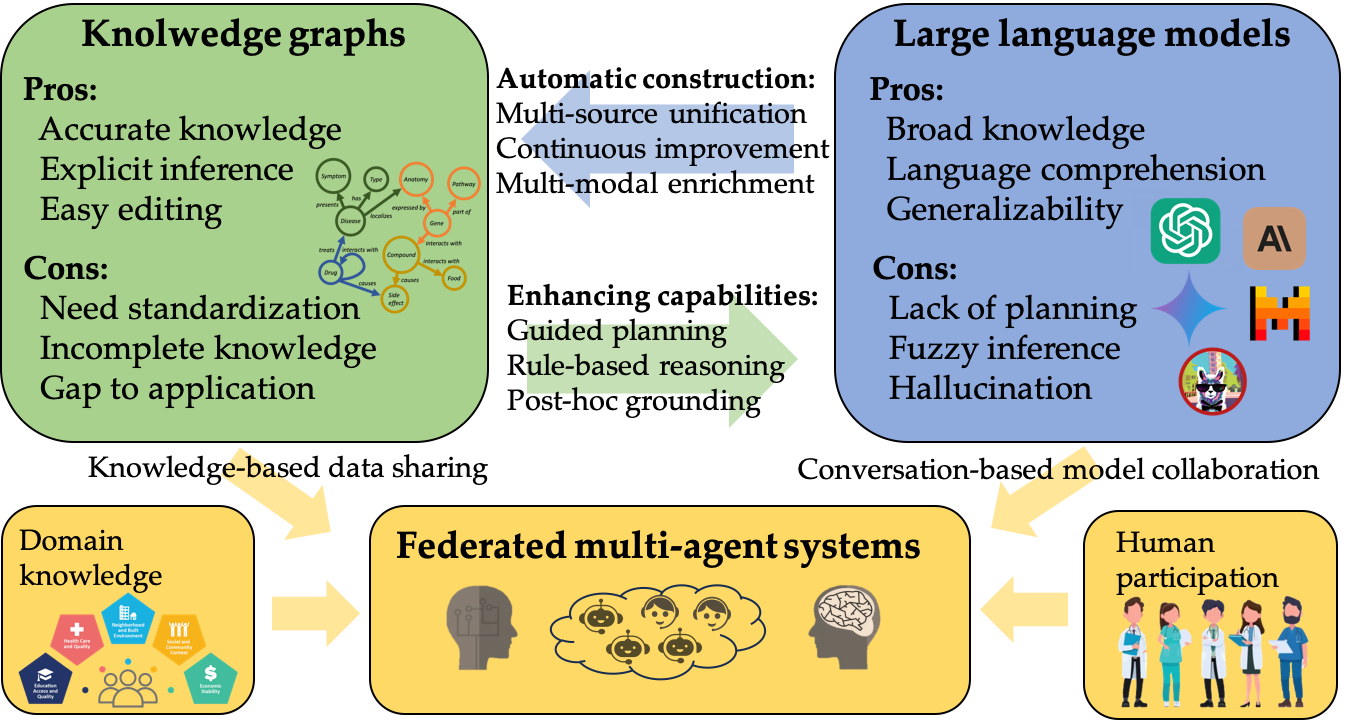
\includegraphics[width=30pc]{submissions/CarlYang2024/figures/intro.png}
\vspace{-3mm}
\caption{Overview of the proposed {knowledge graph and large language model co-learning framework}.}
\vspace{-5mm}
\label{fig:intro}
\end{figure}

%kg+llm existing combinations and limitations
%synergized modeling: roadmap
%KG for LLM: new knowledge, knowledge representation, interpretation-- do not rigorously address the unique challenges in healthcare
%LLM for KG: embedding, completion, construction-- do not comprehensively handle the unique challenges in healthcare
%LLM+KG for health: specific applications without fundamentally improving LLMs and KGs for healthcare
%multi-agent: role play-- do not consider the unique challenges in healthcare regarding privacy, values and disparity
Recently, significant research attention has been drawn to the synergies between KGs and LLMs \cite{pan2023large, pan2024unifying, pan2024integrating, wang2021kepler, yu2022jaket, yasunaga2022deep, jiang2024efficient}, due to their naturally complementary advantages (Figure \ref{fig:intro}). 
The construction and modeling of KGs have often relied on advances in natural language processing (NLP), with recent efforts intensively exploring language models towards the embedding \cite{wang2022language, yu2022cocodr, xie2023lambdakg, choudhary2023complex, zhang2020pretrain, ke2021jointgt}, completion \cite{yao2019kg, kim2020multi, lv2022pre, shen2022joint, choi2023knowledge, wang2021structure, wang2022simkgc, li2023multi, saxena2022sequence, chen2022knowledge, chen2023dipping, lovelace2022framework, xie2022discrimination} and construction \cite{zhu2023llms, ye2022generative, qin2023chatgpt, kommineni2024human, zhang2024extract, vizcarra2024representing, yu2023bear, hu2023llm, meyer2023llm, hofer2024towards, yang2024graphusion, melnyk2021grapher, kumar2020building, chen2022knowprompt, wan2023gpt, wang2024kglink, li2024preliminary, yan2021unified, ding2022prompt, efeoglu2024retrieval, li2022ultra, ayoola2022refined, cattan2021cross, thirukovalluru2021scaling, alt2019improving, guo2021constructing, bosselut2019comet, hao2022bertnet, west2022symbolic} of KGs. 
Studies in the recent years have also bloomed to explore the utilization of KGs for enhancing LLMs through providing new sources of knowledge during pre-training \cite{hu2023survey, wei2021knowledge, yin2022survey, wang2023unifying, sun2022jointlk, liu2021kg, qi2021answering, mavromatis2024gnn, zhang2022greaselm, feng2020scalable, yasunaga2021qa, zhang2019ernie, sun2021ernie, liu2020k, dai2022knowledge, shen2020exploiting, zhang2020bert, tian2020skep, rosset2020knowledge, li2022pre, xiong2020pretrained, he2020bert, su2021cokebert, zhu2023pre, feng2023knowledge, huang2022endowing, agarwal2021knowledge, xu2023kilm, oguz2022unik, tan2024walklm, xu2024bmretriever,sun2020colake, zhang2022dkplm, ye2022ontology, luo2023chatkbqa, martino2023knowledge, chen2020kgpt, santos2022knowledge, moiseev2022skill} or inference \cite{li2023graph, jiang2023unikgqa, luo2024reasoning, sun2024think, wang2024reasoning, luo2023chatrule, wang2023enhancing, besta2024graph, wang2019improving, wang2024knowledge, allemang2024increasing, ji2023rho, feng2023factkb, mcdonald2024reducing, lee2022promptiverse, brate2022improving, wen2023mindmap, wilmot2021memory, logan2019barack, wu2022efficient, guan2024mitigating, dong2024don, sarthi2024raptor, he2024g, han2023pive, edge2024local, gutierrez2024hipporag, liang2024empowering}, and enabling knowledge-based interpretation and evaluation \cite{petroni2019language, jiang2020can, adolphs2021query, shin2020autoprompt, mallen2022not, cohen2023qa, luo2023systematic, liu2023evaluating, orogat2021cbench, zhu2023dyval, bai2024kgquiz, ho2020constructing}. 
Finally, pioneering studies have also been conducted to explore LLM-based multi-agent systems, mostly through prompt-based role-plays to simulate human collaborations \cite{tracy2018agent, tang2024medagents, kaur2024llm, li2024agent, kim2024adaptive, gebreab2024llm, yue2024ct, pan2024agentcoord, xiao2024cellagent}. 

{In this paper, we re-emphasize the promise of KG and LLM co-learning, especially through a structure-oriented retrieval augmented generation (SRAG) paradigm, where LLMs extract structured knowledge from unstructured data, which can be further retrieved to enhance the capabilities and reliabilities of LLMs during applications.}
Specifically, we give examples and discuss several natural and promising use cases where LLMs can be utilized to automate the construction of high-quality KGs. Furthermore, we summarize and highlight several limitations of current LLMs that can be potentially mitigated through the utilization of KGs. Finally, we envision a federated multi-agent system where models and data are disentangled while humans and knowledge are deeply engaged. Future directions are further discussed in the end.
\section{LLM-aided KG Construction}
In this section, we study and establish the advantages of utilizing LLMs for the construction of KGs, by demonstrating their effectiveness in improving the \textit{accuracy}, \textit{consistency}, \textit{coverage}, and \textit{freshness} of knowledge. %Generally speaking, current research and practice on KGs are intensive but mostly around specific types of entities. 
Popular KGs such as Freebase \cite{bollacker2008freebase}, Yago \cite{suchanek2008yago} and Wikidata \cite{vrandevcic2014wikidata} contain hundreds of millions of real-world entities like people, places, and things, along with their multi-typed relations. However, since the KGs are collected and curated by different platforms and institutions, they do not use a unified coding system or thesaurus. The varying terminologies due to different conventions or abbreviations can lead to high degrees of duplication and inconsistency when multiple KGs are directly put together. 
Moreover, the sheer amounts of data in existing KGs are enormous, but the knowledge is still never comprehensive enough to serve various needs of real-world applications, especially those requiring rapidly updated knowledge.
%A few studies have attempted to construct general-purpose healthcare KGs through integrating existing ones \cite{su2023biomedical, cornet2008forty, santos2020clinical}, but they heavily rely on existing coding systems and thesauruses \cite{harrison2021icd, lipscomb2000medical, bodenreider2004unified} for entity alignment across KGs, which often fail in front of varying terminologies such as due to different conventions or abbreviations, leading to high degrees of duplication and inconsistency. 
Recently, pioneering studies including ours have demonstrated strong promise of utilizing LLMs to automate the construction, integration, and enrichment of KGs \cite{zhu2023llms, ye2022generative, qin2023chatgpt, kommineni2024human, zhang2024extract, vizcarra2024representing, yu2023bear, hu2023llm, meyer2023llm, hofer2024towards, yang2024graphusion}. In the following, we give several examples of promising attempts of these kinds and discuss more natural use cases of LLMs and multi-modal foundation models (MMFMs) toward constructing high-quality KGs as promising future directions. 

\subsection{Integrating existing KGs}
% \carl{Need some overviews about motivation, challenge, why LLMs are promising, recent works using LLMs (ours), other recent works, future directions}
%HiPrompt, PromptLink and other LLM-based KG integration
KG integration, also known as knowledge fusion or knowledge alignment, represents a fundamental challenge in the broader landscape of knowledge engineering, which involves integrating multiple KGs that originate from varied sources and formats~\cite{yan2024knownet,lu2022open}.
% The integration of existing KGs presents both great premise and significant challenges in knowledge engineering. 
While individual KGs often excel in specific domains or use cases, their true potential can be unlocked through effective integration, enabling more comprehensive and robust knowledge representation~\cite{himmelstein2017systematic,santos2020clinical}. 
As the number and diversity of KGs continue to grow, the need for effective integration methods becomes increasingly critical.

However, the integration of existing KGs faces several key challenges: (1) \textit{semantic heterogeneity across sources}: Different KGs often use varying terminologies, definitions, and contextual frameworks to represent similar concepts~\cite{liu2022selfkg}; 
(2) \textit{varying granularity levels in knowledge representation}: KGs may differ in the detail and depth with which they describe entities and relationships, impacting the consistency and usability of integrated data. 
Although several neural approaches have been proposed for entity alignment on KGs~\cite{wang2018cross,zhu2020collective,yan2021dynamic}, these methods generally depend heavily on labeled data for training. However, obtaining sufficient labeled data often involves substantial manual effort and can be rather costly.

LLMs have emerged as a promising solution to these challenges with unique advantages: 
First, their strong natural language understanding capabilities enable them to capture semantic relationships among concepts that may be missed by traditional string-matching or embedding-based approaches \cite{chen2023dipping}. 
Second, LLMs can draw on their extensive knowledge acquired during pre-training to aid in disambiguating entities and mapping relationships across different KGs \cite{sancheti2024llm}.
Third, LLMs possess robust few-shot learning abilities, making them particularly valuable for specialized domain applications where labeled data are limited \cite{brown2020language,agrawal2022large}.

\begin{figure}[htbp]
    \begin{center}
    %\framebox[4.0in]{$\;$}
    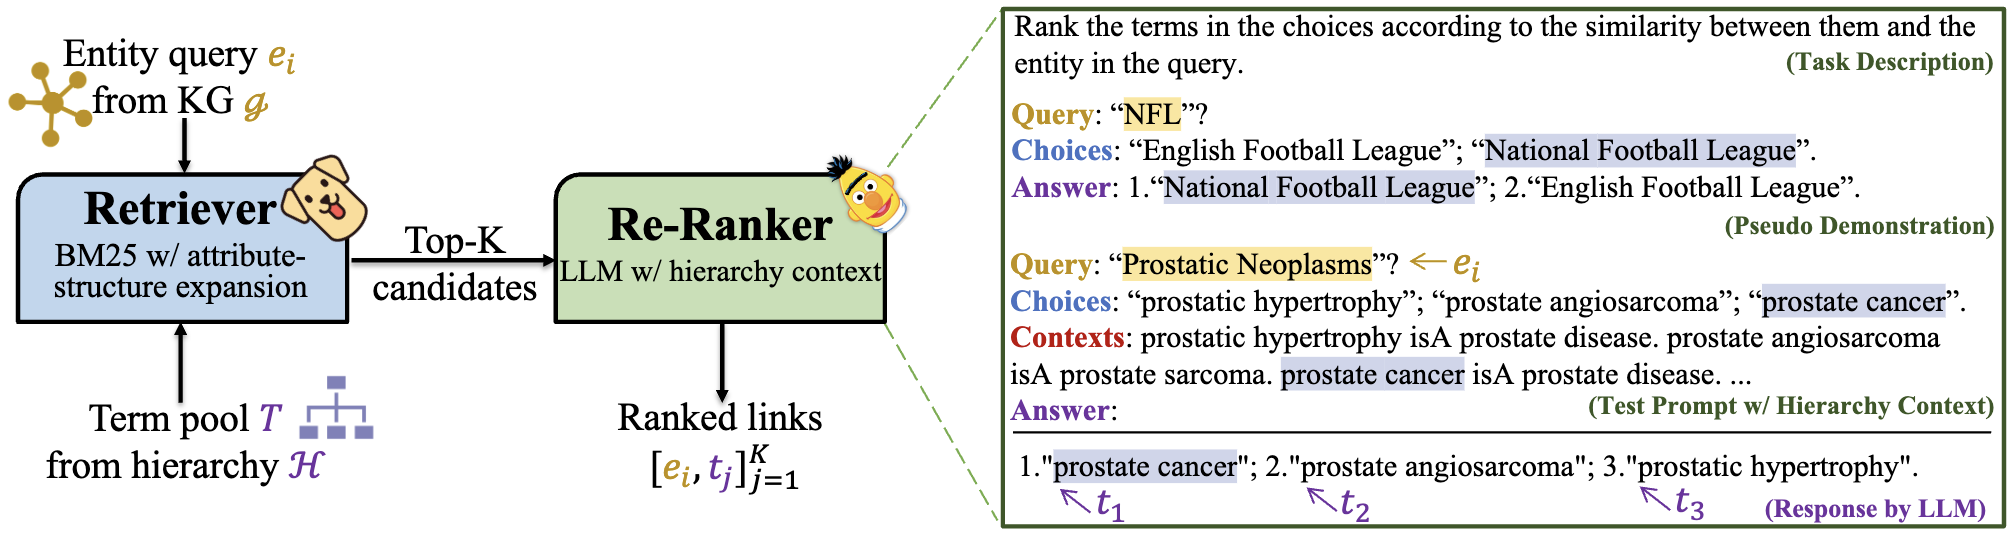
\includegraphics[width=.95\columnwidth]{submissions/CarlYang2024/figures/hiprompt.png}
    \end{center}
    \vspace{-4mm}
    \caption{The overall framework of Hiprompt.}
    \label{fig:hiprompt}
     \vspace{-2mm}
\end{figure}

Recent work has demonstrated the effectiveness of LLM-based approaches in KG integration. 
For example, Lu et al.~\citep{lu2023hiprompt} developed HiPrompt (framework shown in Figure~\ref{fig:hiprompt}), which aligns entities between biomedical KGs and standardized hierarchical entity taxonomies. 
This task poses significant challenges due to the scarcity of available pairs and the inconsistent naming conventions between KGs and entity taxonomies.
Their two-stage approach combines traditional information retrieval techniques (BM25) with LLM-based re-ranking using hierarchy-oriented prompts, achieving superior performance in few-shot biomedical knowledge-graph integration.  
Building on this direction, Xie et al.~\citep{xie2024promptlink} developed PromptLink, a framework that leverages both domain-specific language models and GPT-4 for cross-source biomedical concept linking. The framework employs a two-stage prompting mechanism by first eliciting the biomedical prior knowledge from the LLM for the concept linking task and then enforcing the LLM to reflect on its own predictions to further enhance their reliability. 
PromptLink’s success in zero-shot scenarios illustrates the potential of LLMs to generalize across diverse data sources without extensive training data.

In contrast to the two LLM approaches that primarily use LLMs for ranking candidate sets, AutoAlign \cite{zhang2023autoalign} employs off-the-shelf LLMs to construct a predicate-proximity graph that captures relationships between entity types rather than individual entities. It then aligns the entity embeddings of two KGs into a common vector space by calculating similarity based on entity attributes.


These advances suggest several promising future directions for LLM-aided KG integration. For example, LLMs could potentially facilitate the continuous integration of new knowledge into existing KGs dynamically and automatically by identifying and resolving conflicts between new and existing information, while maintaining consistency across the integrated knowledge base. Such real-time data integration is especially beneficial for dynamic applications like live event monitoring and real-world decision-making. {Furthermore, integrating KGs with LLMs remains challenging due to the risk of generating false or untrustworthy information~\cite{yang2024give}. To mitigate this issue, there is a growing need for improved human-in-the-loop systems. Specifically, enhanced interfaces~\cite{hassan2017claimbuster,nakov2021automated} can enable experts to more effectively verify and interpret LLM-generated recommendations, ensuring greater reliability and transparency.}



% Lu et al.~\citep{lu2023hiprompt} propose HiPrompt, an innovative framework that leverages LLMs for biomedical knowledge fusion. Their work addresses the challenge of aligning entities from biomedical KGs with terms in a standardized hierarchical index system, a task that traditionally suffers from scarce labeled data and inconsistent naming conventions. HiPrompt employs a two-stage approach: a retrieval module using BM25 with expanded entity and term representations, followed by an LLM-based re-ranking module that utilizes hierarchy-oriented prompts. This approach enables effective few-shot learning, outperforming both conventional unsupervised methods and neural embedding models in zero-shot and one-shot settings. It demonstrates the potential of LLMs in capturing complex semantic relationships and hierarchical constraints in KG integration tasks, even with minimal supervision. Their findings suggest that LLM-aided approaches could significantly advance the field of KG construction and integration, particularly in domains with limited labeled data.

% Another notable example is PromptLink~\citep{xie2024promptlink}, which leverages LLMs for cross-source biomedical concept linking. PromptLink combines the strengths of biomedical-specialized pre-trained language models and GPT-4 to address the challenges of inconsistent naming conventions across different data sources. The framework employs a two-stage prompting mechanism that efficiently filters candidates and generates reliable linking predictions, including NIL predictions when no suitable match is found. By outperforming conventional string-matching and machine learning-based methods in zero-shot accuracy, PromptLink demonstrates the potential of LLMs in enhancing KG integration tasks. This approach is particularly valuable in domains where labeled data is scarce and the ability to generalize across various data sources is crucial.

\subsection{Constructing and Completing KGs}
KGs have high-standard requirements on the quality of knowledge, regarding accuracy, consistency, coverage and freshness. No matter constructed through manual curation, NLP tools, or their combinations, KGs can unavoidably include erroneous knowledge. Moreover, when multiple KGs are integrated, conflicting knowledge can emerge. Finally, new knowledge is constantly generated from new experiments and research, making existing knowledge inaccurate and incomplete. LLMs have emerged as a promising solution, leveraging the vast and adaptable knowledge acquired during pre-training to overcome these limitations \cite{petroni2019language, yu2024kola, xu2024clingen, alkhamissi2022review}. 
The key advantage of LLMs for KG construction and completion is their ability to generate novel, semantically coherent information with minimal reliance on additional labeled data.

% The key advantage of LLMs in this domain lies in their ability to generate novel, semantically coherent information that can supplement and enrich existing KGs. Unlike rule-based or supervised machine learning approaches, LLMs can leverage their extensive understanding of language and the world to infer missing connections, identify new entities, and uncover implicit relationships - all without being constrained by the limitations of manually curated training data.

Recent studies have highlighted the effectiveness of LLM-based approaches for KG construction and completion. Zhu et al. \citep{zhu2023llms} utilize in-context learning capabilities of LLMs to complete tuples with missing entities or relations to generate new knowledge triplets for augmenting existing KGs.
Wei et al. \citep{wei-etal-2023-kicgpt} and Wang et al. \citep{wang-etal-2024-kc} tackle KG completion as a candidate identification and ranking task, proposing a “retrieve-rank” pipeline where LLMs are used to rerank top-retrieved entities, thus creating additional knowledge triplets.

An alternative approach to prompting LLMs involves using code-based prompts,  rather than natural language, to incorporate new entities into existing KGs~\cite{bi2024codekgc,zeng2024codetaxo}. 
Code LLMs, extensively trained on structured data such as programming code, are inherently well-suited to the structured nature of KGs.
Using a code-based interface enables more effective handling of graph-like structures, logical relationships, and precise reasoning~\cite{madaan2022language,chen2023program,shi2024agent}.
Specifically, Bi et al. \cite{bi2024codekgc} first encoded the schema of KGs by modeling code definitions, to capture the structural information inherent in the data. They then employed chain-of-thought prompting to produce accurate knowledge triples. This methodology demonstrates improved performance over traditional natural language-based prompts. 
Similarly, Zeng et al.~\citep{zeng2024codetaxo} proposed CodeTaxo, which represents entities within a base 'Entity' class, mirroring hierarchical relationships in programming constructs. This approach enables LLMs to efficiently create taxonomic structures by leveraging syntactic capabilities commonly used in code tasks, thus enhancing the organization and completeness of KGs. 
% Another notable example is CodeTaxo~\citep{zeng2024codetaxo} which encapsulates entities in a base class 'Entity' to better characterize hierarchical relations similar to programming constructs. This enables the LLM to efficiently process and generate taxonomic structures by leveraging its strong syntactic capabilities, which are typically associated with code understanding tasks. By combining the LLM's natural language understanding with its code-related skills, CodeTaxo demonstrates the versatility of these models in enhancing the completeness and organization of KGs.


The above methods primarily focus on prompting LLMs for KG construction and completion. While these methods show promise, they fall short in fully adapting LLMs to target tasks and can suffer from hallucination issues. To address these limitations, several studies aim to improve the quality of LLM-generated content for KG tasks. 
{Zhang et al. \cite{zhang2024extract} presented a three-phase framework for constructing KGs with LLMs to enhance contextual understanding and schema alignment. 
It starts with open information extraction to identify relation triplets from unlabeled textual corpora, followed by schema definition where LLMs generate contextually relevant descriptions for schema components. 
Finally, the extracted triplets are aligned with the schema.  
To further enhance the quality of the extracted
triplets and minimize the risk of misinformation, a schema retriever is used to generate a list of candidate entities and relations to guide the triplet extraction steps. This approach works for both predefined schemas and situations where the schema needs to be inferred from the context.
}
% \cite{zhang2024extract} presents a three-phase framework for constructing KGs with LLMs to enhance contextual understanding and schema alignment. The process begins with open information extraction, where relational triplets are identified from unlabeled textual corpora. Next, LLMs is used to define schema components by generating contextually relevant, human-like descriptions. In the final canonicalization phase, extracted triplets are aligned with the schema to ensure consistency and reduce redundancy. This adaptable framework is effective in both predefined schema settings and scenarios where schema must be inferred from context.
Additionally, various studies explored fine-tuning LLMs specifically for KG completion. Zhang et al.~\cite{kopa} proposed KOPA that first applies structural pre-training to create embeddings of entities and relations in KGs, and project embeddings into the textual space as virtual knowledge tokens. These tokens act as prefixes in LLM input prompts, enabling structure-aware reasoning that leverages both the generative power of LLMs and the retrieval of structured KG information to improve the accuracy and completeness of KG completion tasks. 
Jiang et al.~\citep{jiang2024kg} introduced KG-FIT for using open-world knowledge from LLMs to enhance KG embeddings. It initially constructs a semantically coherent, hierarchical structure of entity clusters, guided by LLM-powered entity representations. It then fine-tunes these embeddings by integrating the hierarchical structure with textual embeddings. This hybrid approach allows KG-FIT to capture both the semantic depth of LLMs and the structural information intrinsic to KGs, resulting in more comprehensive KG representations.



% TaxoPrompt~\citep{xu2022taxoprompt}, a prompt-based method for self-supervised taxonomy expansion that effectively leverages the global structure of taxonomies. TaxoPrompt integrates the taxonomic context into the training of a language model (LM) by employing a customized random walk algorithm that captures relational paths within the taxonomy. This context is then used in a prompt-tuning framework to transform the taxonomy expansion problem into a hypernym generation task. During the process, a template creates a cloze task where the LM predicts missing hypernyms based on provided context, thus maintaining the structural integrity of the taxonomy.


% https://arxiv.org/abs/2405.16412
% https://dl.acm.org/doi/pdf/10.1145/3637528.3671469
% https://arxiv.org/pdf/2408.09070
% https://www.ijcai.org/proceedings/2022/0615.pdf

\begin{figure}[htbp]
    \begin{center}
    %\framebox[4.0in]{$\;$}
    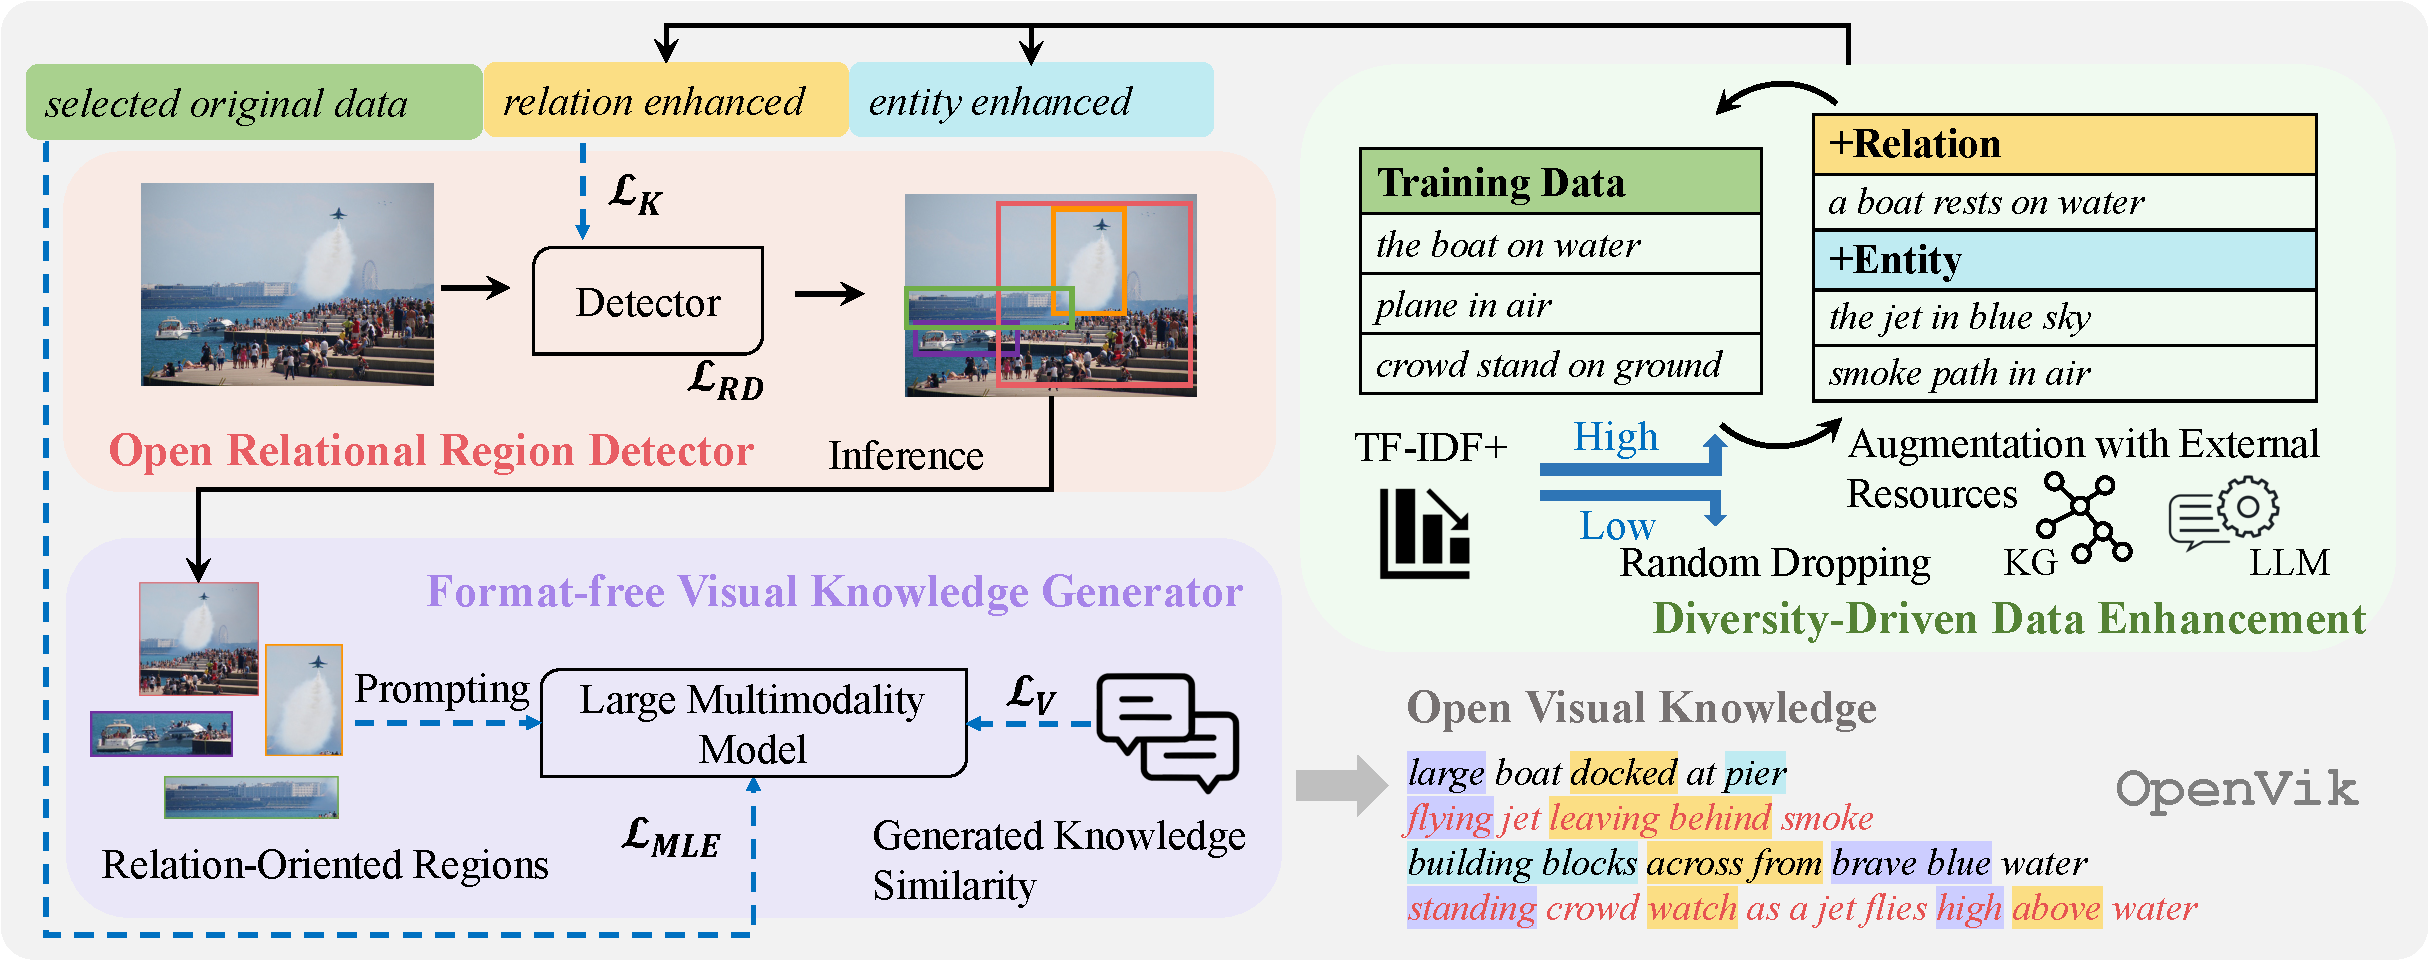
\includegraphics[width=.95\columnwidth]{submissions/CarlYang2024/figures/openvik.pdf}
    \end{center}
    % \vspace{-3mm}
    \caption{{The overall framework of OpenVik consists of two main components: (1) an open relational region detector, highlighted in the orange and purple panels, which includes a region regression loss ($\mathcal{L}_{\text{RD}}$) and a regional description loss ($\mathcal{L}_{\text{K}}$), and (2) a format-free visual knowledge generator, incorporating knowledge generation loss ($\mathcal{L}_{\text{MLE}}$) and diversity regularization ($\mathcal{L}_{\text{V}}$). These modules work collaboratively to extract open visual knowledge, incorporating novel entities and diverse relations in a format-free manner.}}
    \label{fig:openvik}
    % \vspace{-5mm}
\end{figure}



\subsection{Enriching KGs with multi-modality data}
Traditionally, specialized models and algorithms have been developed to process and analyze various modalities of data such as tables, texts, images, and time series. These methods can hardly perform integrative analysis across data modalities and generalize across different data platforms. Recently, LLM-based multi-modality foundation models (MMFMs) have shown strong promise in analyzing multi-modality data through the unified interface of languages \cite{yang2023dawn, fei2022towards, li2024multimodal, li2024llava, zhang2023biomedgpt}.
Integrating multi-modal data into KGs creates a more comprehensive representation of entities and their relationships, enhancing performance in open-world applications like image classification and visual question answering \cite{chen2024knowledge}. Many studies focus on using MMFMs for specific tasks, such as entity extraction \cite{sun2024umie,li2023prompting,hu2023prompt}, relation extraction \cite{yu2023visually,li2024zero,li2024pixels}, or event extraction \cite{chen2024schema,rasheed2024glamm}. However, these works often isolate extraction tasks without unifying entities and relations into a structured KG.
{A pioneering approach in this direction is OpenVik \cite{cui2024open} (framework shown in Figure~\ref{fig:openvik}). It first trains an open relational region detector to locate image regions containing relational information. 
It then employs a visual knowledge generator to create format-free knowledge descriptions by prompting a large visual language model. Through the use of MMFM, OpenVik advances KG completion by integrating rich visual context, expanding knowledge coverage, and enhancing the accuracy of representation within the resulting KG.}
Application-wise, Yang et al.~\cite{yang2024hierarchical}  proposed an automated approach to constructing product KGs from raw images in e-commerce. This method first employs vision-language models (VLMs) to extract detailed image information and then uses an LLM to reason and infer additional KG properties not visually present, hierarchically expanding, and linking nodes to develop comprehensive, scalable KGs without human input.


% https://www.cs.emory.edu/~jyang71/files/openvik.pdf
\newcommand{\gG}{\mathcal{G}\xspace}
\newcommand{\gL}{\mathcal{L}\xspace}
\newcommand{\gZ}{\mathcal{Z}\xspace}

\section{KG-guided LLM Enhancement}
LLMs have shown impressive communication and question-answering capabilities, demonstrating strong promise in various applications \cite{wang2024survey, wu2023bloomberggpt, cui2023chatlaw, chen2023genept, singhal2023large, singhal2023towards, haupt2023ai, nori2023capabilities, lee2023benefits, fleming2023assessing, chen2023meditron, yang2022large, luo2022biogpt, agrawal2022large, mehandru2024evaluating, zhang2023biomedgpt, biswas2023role, dash2023evaluation}. 
%answering medical questions \cite{singhal2023large, singhal2023towards, haupt2023ai, nori2023capabilities, lee2023benefits, fleming2023assessing, chen2023meditron}, extracting clinical information \cite{yang2022large, luo2022biogpt, agrawal2022large} and assisting clinical decisions \cite{mehandru2024evaluating, zhang2023biomedgpt, biswas2023role, dash2023evaluation}. 
%However, LLMs are also shown to ``hallucinate'' false outputs and unsubstantiated answers \cite{hal, hal3, hal4}, preventing their adoption in diverse fields, especially those with high-standard requirements on the accuracy and factuality of responses such as healthcare \cite{hal7}. Recently, many technical frameworks have been proposed to detect or avoid hallucinations in LLMs, such as based on supervision for reinforcement learning \cite{hal8}, statistical uncertainty measurements \cite{hal} and \todo{xxx \cite{}}. 
However, to reliably model domain-specific data and generate factual and accurate answers, LLMs still face the challenges of lacking domain knowledge, fuzzy inferences, and hallucination \cite{hu2023large, mousavi2024your, yadkori2024believe, asai2024selfrag,yu2024rankrag, liu2023evaluating, zhu2023dyval, zhuo2024roles, yuan2024back, wang2023boosting, ji2023survey, bai2024hallucination, tonmoy2024comprehensive, maynez2020faithfulness, xiao2021hallucination, farquhar2024detecting, ji2023towards, chen2024inside}.
% \textit{lack of knowledge} \cite{hu2023large, mousavi2024your, xu2024kg, becker2024cycles, yadkori2024believe, kim2024m}, \textit{fuzzy inference} \cite{liu2023evaluating, zhu2023dyval, bai2024kgquiz, zhuo2024roles, baek2024researchagent, yuan2024back, wang2023boosting}, and \textit{hallucination} \cite{ji2023survey, bai2024hallucination, tonmoy2024comprehensive, maynez2020faithfulness, xiao2021hallucination, farquhar2024detecting, ji2023towards, chen2024inside}
Retrieval augmented generation (RAG) \cite{lewis2020retrieval}, which aims at retrieving query-relevant evidence and generating evidence-based answers, has strong promise in evidence-critical domains. However, effective and efficient RAG for complex queries is still challenging which requires LLMs to be able to (1) generate logical plans for retrieving multiple pieces of relevant evidence from complex data, (2) conduct valid reasoning and inference to compose the pieces of evidence towards generating coherent answers, and (3) reliably guarantee the detection and removal of errors. In the following, we discuss how these challenges can be addressed with well-designed planning, reasoning, and reflection frameworks with the help of KGs.

{
\newcommand{\ourmethod}{\texttt{RoG}\xspace}
\subsection{Planning with domain knowledge}
% \carl{Linhao, the current 3.1 is too long-- we aim to write about 12 pages of main contents in total and the plan is to write about 2 (front page/intro)+ 3 (sec 2) + 3 (sec 3) + 2 (sec 4) + 1 (sec 5) + unlimited references. Can you perhaps try to separate the current contents into 3.1 (planning) and 3.2 (reasoning)? Please try to re-organize/re-write the contents more so they also read differently from your RoG paper. Please also add some discussions about more related recent works separately in both subsections. I added a reference in 3.3, but please let me know if you are not sure about what to write in 3.3. Thanks!}\\
While LLMs excel in many NLP tasks \cite{brown2020language,bang2023multitask}, they still face challenges in acquiring domain knowledge. To address this issue, many attempts seek assistance from KGs, which are often constructed to represent knowledge in specific domains, such as medicine \cite{bodenreider2004unified}, law \cite{kang2024bridging}, and finance \cite{liu2019anticipating}. The integration of KGs and LLMs has shown promising results in various applications, such as question answering \cite{jiang2023unikgqa}, recommendation \cite{wang2023enhancing}, and dialogue systems \cite{tuan2022towards}. Despite the success, there are still challenges in effectively obtaining useful information from KGs and incorporating them into LLMs. 

Existing methods typically depend on a retriever to obtain relevant triples. For example, Baek et al. \cite{baek2023direct} proposed a direct retrieval method to retrieve relevant triples from KGs. However, the retriever may not always retrieve the most relevant triples, leading to suboptimal performance. Additionally, KGs contain a wealth of domain-specific knowledge, making it challenging for LLMs with limited domain expertise to comprehend and utilize this information. To further unleash LLMs' capabilities of leveraging domain knowledge, the \textit{plan-and-solve} paradigm \cite{wang2023plan} has been proposed, in which LLMs are prompted to first generate a plan. Based on the plan, LLMs can retrieve the relevant domain knowledge and conduct reasoning to generate answers \cite{yaoreact}. However, existing methods are incapable of handling the complex structured knowledge in KGs to enable effective planning and reasoning. To address this issue, we propose a \textit{planning-retrieval-reasoning} framework named \ourmethod that enables LLMs to plan and reason on KGs \cite{luo2024reasoning}. The overall framework is illustrated in \Cref{fig:rog}.

\begin{figure}[htbp]
    \begin{center}
    %\framebox[4.0in]{$\;$}
    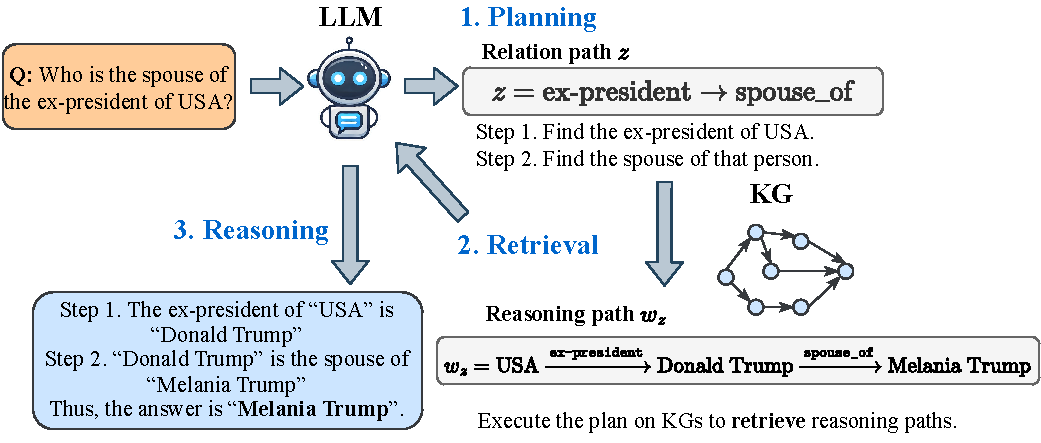
\includegraphics[width=.85\columnwidth]{submissions/CarlYang2024/figures/rog.pdf}
    \end{center}
    % \vspace{-3mm}
    \caption{The overall framework of planning and reasoning on KGs (\ourmethod).}
    \label{fig:rog}
    % \vspace{-5mm}
\end{figure}

\ourmethod first generates several relation paths that are grounded by KGs as plans. Relation paths, which capture semantic relations between entities, have been utilized in many reasoning tasks on KGs \cite{wang2021relational,xusubgraph}. Based on relation paths, we can always retrieve the latest knowledge from KGs with a simple constrained breadth-first search. Therefore, relation paths can serve as faithful plans to guide the retrieval and reasoning on domain-specific KGs. Additionally, by treating relation paths as plans, we can make sure the plans are grounded by KGs, which enables LLMs to retrieve relevant knowledge and conduct faithful reasoning. To this end, we formulate our \ourmethod as an optimization problem that aims to maximize the probability of reasoning the answer from a KG $\gG$ w.r.t the question $q$ by generating relation paths $z$ as the plan:
\begin{equation}
    % \setlength\abovedisplayskip{1pt}%shrink space
    % \setlength\belowdisplayskip{1pt}
    \label{eq:plan}
    P_\theta(a|q,\gG) = \sum_{z\in\gZ}P_\theta(a|q,z,\gG)P_\theta(z|q),
\end{equation}
where $\theta$ denotes the parameters of LLMs {and $a$ denotes the final answer.} To enable accurate planning with domain knowledge, we design two instruction tuning tasks: 1) \textit{planning optimization}, which distills the knowledge from KGs into LLMs to generate faithful relation paths as plans; 2) \textit{retrieval-reasoning optimization}, which enables LLMs to reason based on the retrieved reasoning paths.
{
The final objective function of \ourmethod is the combination of the planning optimization and retrieval-reasoning optimization, which can be formulated as
\begin{equation}
    \setlength\abovedisplayskip{1pt}%shrink space
    \setlength\belowdisplayskip{1pt}
    \label{eq:final_obj}
    \gL = \log \underbrace{P_\theta(a|q,\gZ^*_K,\gG)}_{\text{Retrieval-reasoning}} + \underbrace{\frac{1}{|\gZ^*|}\sum_{z\in Z^*}\log P_\theta(z|q)}_{\text{Planning}},
\end{equation}
where we use the shortest paths $\gZ^*\subseteq\mathcal{Z}$ between $q$ and $a$ in KGs as supervision signals. We maximize the probability of LLMs generating faithful relation paths through distilling the knowledge from KGs.
}
In this way, with the proposed \ourmethod, LLMs can effectively retrieve domain knowledge from KGs with planning, which significantly enhances the reasoning capability of LLMs.
}

{
    \newcommand{\ourmethod}{\texttt{GCR}\xspace}
\subsection{Reasoning with structured knowledge}
% https://arxiv.org/abs/2410.13080
KGs capture abundant factual knowledge in a structured format, which provides a faithful knowledge source for improving the reasoning abilities of LLMs \cite{pan2024unifying}. Nevertheless, because of the unstructured nature of LLMs, directly applying them to reason on structured KGs is challenging. Early works focus on fine-tuning LLMs together with structured knowledge from KGs to enrich the knowledge of LLMs for better reasoning \cite{zhang2019ernie,rosset2020knowledge}. For example, KEPLER~\cite{wang2021kepler} directly employs both KG embedding training objective and Masked token pre-training objective into a shared transformer-based encoder. Through fine-tuning, LLMs can better understand the structured knowledge in KGs for reasoning. However, the fine-tuning process is computationally expensive and incapable of efficiently adapting to the evolving real-world knowledge. 

Recently, researchers have combined the strengths of retrieval-based methods with the prompting technique to enable LLMs to reason on KGs \cite{lewis2020retrieval,jiang2023unikgqa}. CoK \cite{wang2023boosting} and KD-CoT \cite{wang2023knowledge} retrieve facts from an external KG to guide the CoT performed by LLMs. To capture graph structure, GNN-RAG \cite{mavromatis2024gnn} adopts a lightweight graph neural network to effectively retrieve knowledge from KGs, which are formatted as a sentence path to elicit the reasoning process of LLMs. Mindmap \cite{wen2023mindmap} builds a prompt-based method that endows LLMs with the capability of comprehending KG and reasoning with it. Despite the success of these methods, they still face challenges in designing principled prompts to represent KGs and conduct reasoning. Moreover, LLMs still have limited capabilities in understanding the graph structure and reasoning with the text-based graph prompts \cite{huang2024can}. 

Different from existing efforts that require a computationally expensive fine-tuning phase or design ad-hot prompts for LLMs,  we recently introduced a KG-constrained reasoning (\ourmethod) paradigm \cite{luo2024graph}. \ourmethod connects unstructured reasoning in LLMs with structured knowledge in KGs, seeking to achieve efficient and effective reasoning on structured knowledge. The overall framework is illustrated in \Cref{fig:gcr}.

\begin{figure}[htbp]
    \begin{center}
    %\framebox[4.0in]{$\;$}
    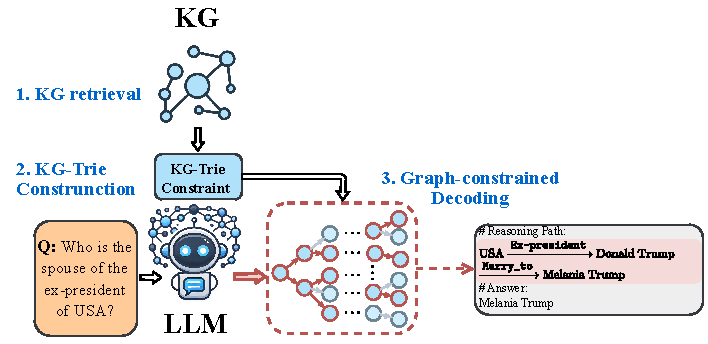
\includegraphics[width=.75\columnwidth]{submissions/CarlYang2024/figures/gcr.pdf}
    \end{center}
    % \vspace{-3mm}
    \caption{The overall framework of KG-constrained reasoning (\ourmethod).}
    \label{fig:gcr}
    % \vspace{-5mm}
\end{figure}

Graph-constrained reasoning, inspired by the concept that LLMs reason through decoding \citep{wei2022chain}, incorporates the KG structure into the LLM decoding process. This enables LLMs to directly reason on graphs by generating reliable reasoning paths grounded in KGs that lead to correct answers. Specifically, given a question, we first adopt a retrieval module to find a relevant KG that is helpful for reasoning. Then, we convert the KG into a structured index, KG-Trie, to facilitate efficient reasoning on KG using LLMs. Trie is also known as the prefix tree \citep{fredkin1960trie} that compresses a set of strings, which can be used to restrict LLM output tokens to those starting with valid prefixes. KG-Trie encodes the reasoning paths in KGs as formatted strings to constrain the decoding process of LLMs. Then, we propose graph-constrained decoding that employs a lightweight KG-specialized LLM to generate multiple KG-grounded reasoning paths and answers. With the constraints from KG-Trie, we ensure faithful reasoning while leveraging the strong reasoning capabilities of LLMs to efficiently explore paths on KGs in constant time. In this way, \ourmethod bridges the gap between structured knowledge in KGs and unstructured reasoning in LLMs, allowing for efficient reasoning on KGs via LLM decoding.

}
\subsection{Reflecting with atomic knowledge}
% \carl{https://arxiv.org/abs/2311.13314}\\
% https://arxiv.org/pdf/2310.11638\\
% https://arxiv.org/pdf/2402.11199\\
LLMs have shown impressive capabilities in encapsulating massive knowledge and conducting reasoning. However, they still face challenges in generating factually correct and faithful responses, especially in the presence of hallucinations \cite{huang2023survey}. KGs store atomic knowledge in a structured format, which can be used to verify the correctness of generated responses and detect hallucinations \cite{agrawal2023can}. To incorporate the factual knowledge from KGs into LLM hallucination detection, Guan et al. \cite{guan2024mitigating} proposed a retrieval-based method called KG-based retrofitting (KGR). KGR retrieves relevant facts from KGs during the LLM reasoning process, which are used to mitigate factual hallucination by retrofitting the initial responses. KGR enables an autonomous knowledge verifying and refining procedure with the factual knowledge retrieved from KGs, which significantly improves the reliability of LLMs. 

The hallucination of LLMs is usually attributed to the lack of factual knowledge of LLMs. To systematically evaluate the factual knowledge inside LLMs, as shown in \Cref{fig:reflecting}a, we propose a novel framework to automatically assess the factual knowledge in LLMs by using KGs \cite{luo2023systematic}. Unlike conventional methods that rely on human-annotated question-answering datasets, we systematically generate valid and diverse questions from KGs
with different difficulties while also ensuring knowledge coverage. Specifically, we retire the atomic knowledge from KGs as sets of triples. Then, we utilize different question generation methods, e.g., template-based and LLM-based methods, to convert the triples into question-answer pairs. The generated pairs are used to evaluate the factual knowledge of LLMs by comparing the generated answers with the ground-truth answers. The evaluation results can be used to reflect the factual knowledge of LLMs. In this way, we can systematically evaluate the factual knowledge of LLMs and provide insights into the hallucination behavior of LLMs, which can be used to improve the reliability of LLMs in various applications. 

Apart from the factual knowledge, the structure of KGs can be also utilized to justify the reasoning process of LLMs. Minh-Vuong et al \cite{nguyen-etal-2024-direct} designed a framework that delves deeper into the CoT reasoning capabilities of LLMs in multi-hop question answering by utilizing KGs, as shown in \Cref{fig:reflecting}b. The framework contains two evaluation modules: discriminative evaluation and generative evaluation. The discriminative evaluation aims to analyze whether the LLMs possess enough knowledge to conduct faithful reasoning. It feeds both valid and invalid reasoning paths retrieved from KGs into LLMs and asks them to predict the validity of these paths. The generative evaluation, on the other hand, aims to evaluate the faithfulness of the reasoning process of LLMs by grounding it on KGs. Given a reasoning process generated by LLMs, the generative evaluation module retrieves the facts from KGs, which are compared with the ground-truth reasoning paths. The evaluation results can be used to reflect the reasoning capabilities of LLMs and provide insights into the faithfulness of LLM reasoning. Based on the findings, although LLMs have shown impressive reasoning capabilities, they still face challenges in conducting faithful reasoning, especially in multi-hop question answering. 

\begin{figure}[htbp]
    \begin{center}
    %\framebox[4.0in]{$\;$}
    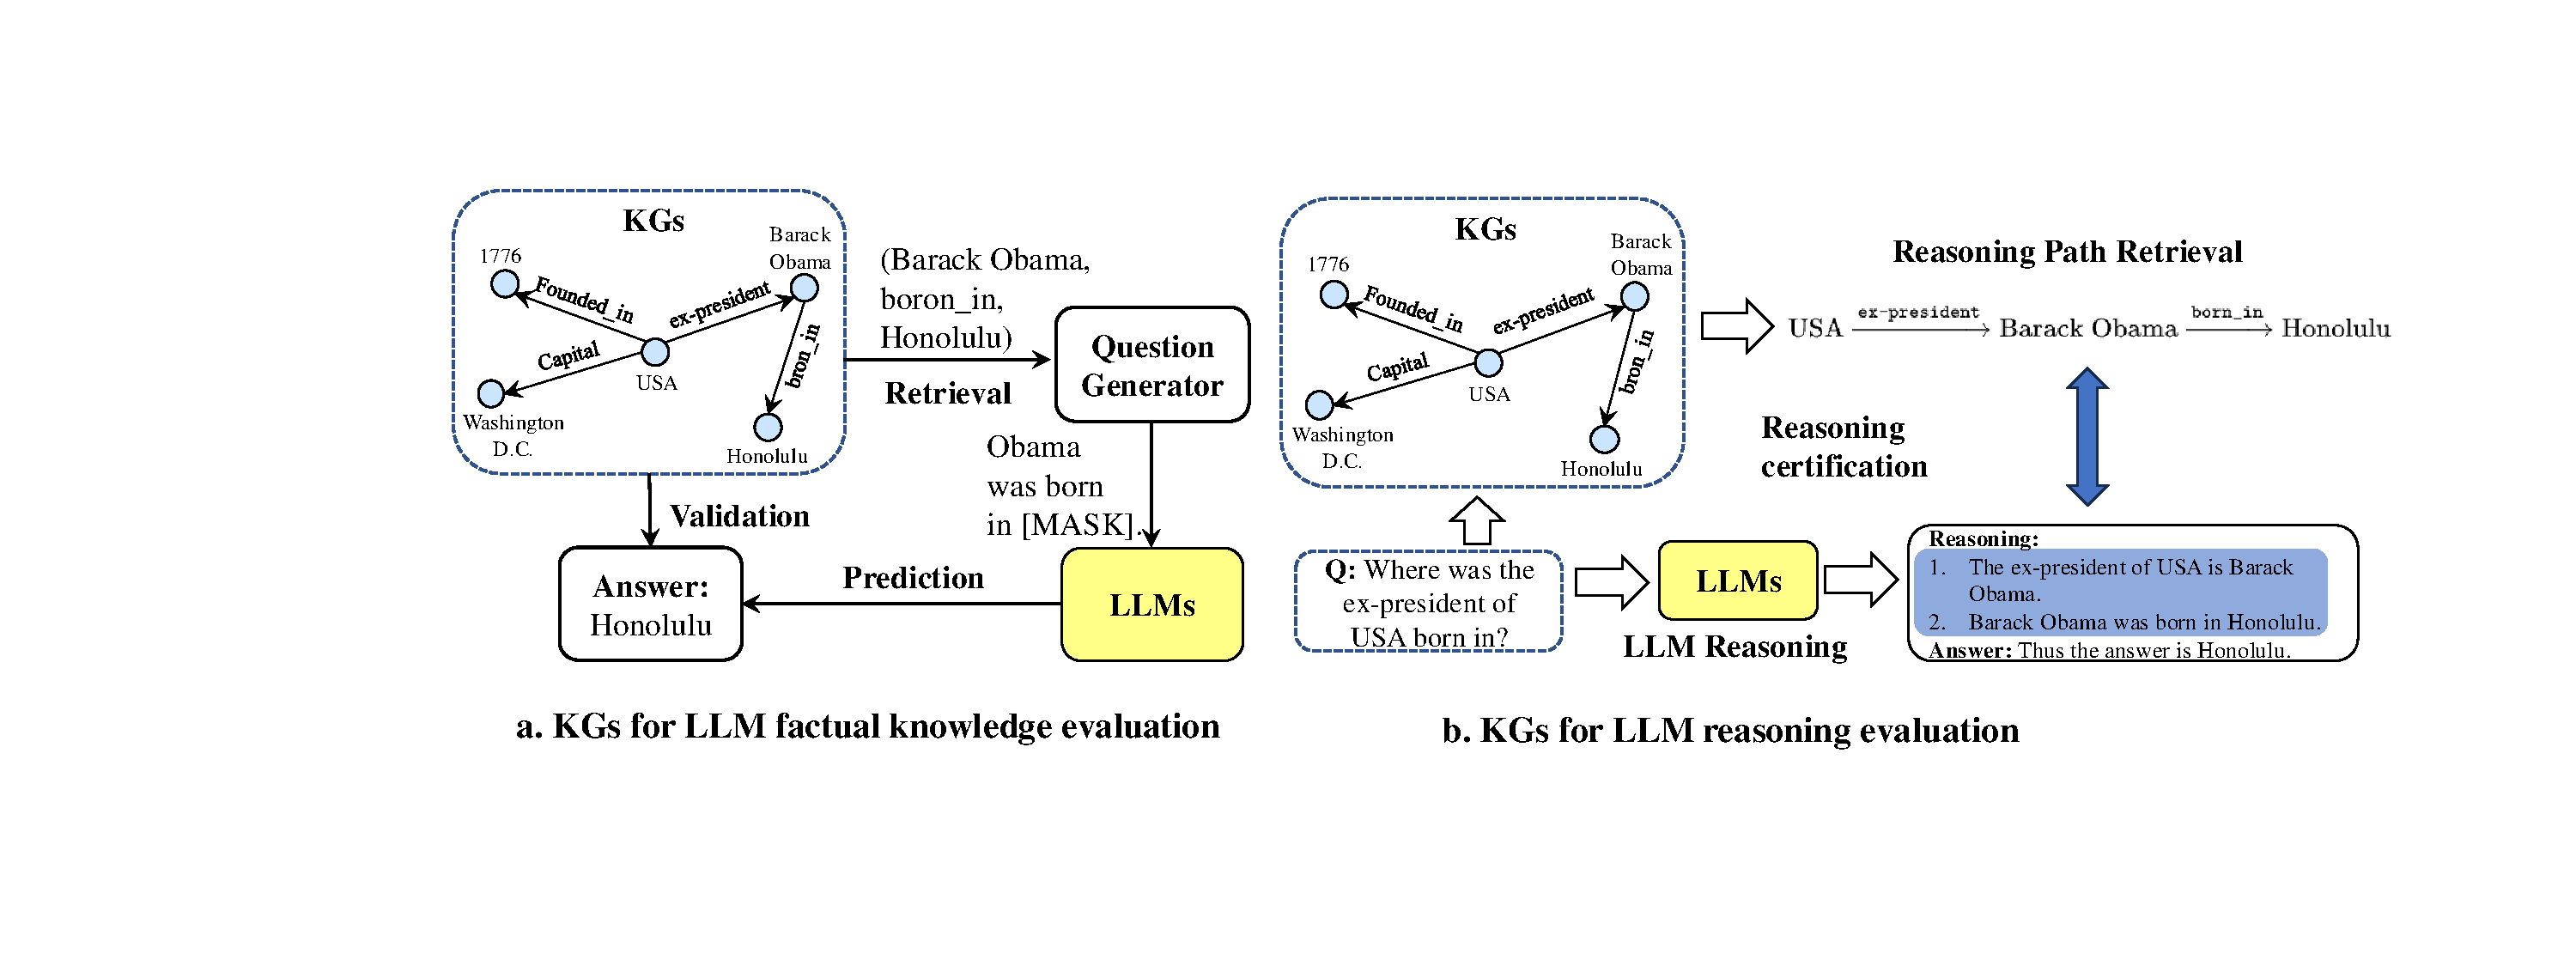
\includegraphics[width=1\columnwidth]{submissions/CarlYang2024/figures/reflecting.pdf}
    \end{center}
    % \vspace{-3mm}
    \caption{The illustration of LLM reflection with KGs. (a) The evaluation of the factual knowledge inside LLMs. (b) The evaluation of the reaosning process of LLMs with KGs.}
    \label{fig:reflecting}
    % \vspace{-5mm}
\end{figure}
\section{Knowledge-aware Multi-agent Federation}
%\carl{TODO: will work on this section over the weekend}\\
While KGs and LLMs can mutually enhance each other, data are properties and many real-world datasets are privately collected and owned by different institutions, which cannot be simply put together to train more powerful models. 
Moreover, many real-world applications require domain-specific knowledge that may not have been captured by general-purpose KGs and LLMs yet, and such knowledge can also be private properties. 
Finally, while the development of KGs and LLMs is highly automated and data-driven, the values and needs of different human stakeholders may not have been properly reflected in the data and models. 
Federated learning (FL) provides a robust and principled framework for privacy-protected multi-site collaboration, but proper implementation of FL in the new era of generative AI remains unclear; the further incorporation of domain knowledge and human participation is also highly under-explored. In the following, we will envision an innovative Federated Multi-Agent System (FedMAS) for multi-site privacy-protected, knowledge-infused, and human-engaged KG-LLM co-learning scenarios. 


Nowadays, while common practices in AI applications still largely resort to in-house development of models based on public and local data, the successes of generative AI, where complex models are trained with large-scale data, have demonstrated a strong need to collaboratively utilize local data towards obtaining powerful models that can generalize across institutions, finding and utilizing deep data patterns underlying common and rare use cases. Towards protecting local data privacy during collaborative model training, FL provides a promising solution \cite{nguyen2022federated, antunes2022federated, nguyen2022federated, antunes2022federated, xu2021federated, rieke2020future}. However, existing FL frameworks, by merely preventing the direct sharing of training data, are not effective in the scenarios of KG-LLM co-learning, because (1) as the construction of comprehensive KGs necessitates the incorporation of knowledge discovered from local data, private information may get reversely inferred from the collaboratively constructed KG; (2) as powerful generative models like LLMs can easily memorize training data, collaboratively trained LLMs may expose private information facing deliberately composed jailbreaking prompts \cite{wei2024jailbroken, wang2023decodingtrust, xu2024llm}.

In our pioneering studies on FL for graphs \cite{he2021fedgraphnn, xie2021federated, zhang2021subgraph, zhang2024deep, xie2023federated, zhang2022efficient, gu2023dynamic, xie2024federated}, we developed several novel algorithms for different graph separation scenarios. In FedDEP \cite{zhang2024deep}, we developed a prototype-based embedding sharing algorithm with local graph differential privacy (DP) guarantees, and demonstrated its utility in FL for global graph embedding models across private local subgraphs; in FedR \cite{zhang2022efficient}, we showed that sharing relation embeddings across local KGs can help FL for global KG embeddings with less privacy leakage. These studies have laid the foundations for our envisioned framework here, which will build on the private embedding sharing algorithms to construct \textit{multi-view KGs} that can facilitate multi-site knowledge sharing with minimum risks of exposing local private data.

\begin{figure}[htbp]
    \begin{center}
    %\framebox[4.0in]{$\;$}
    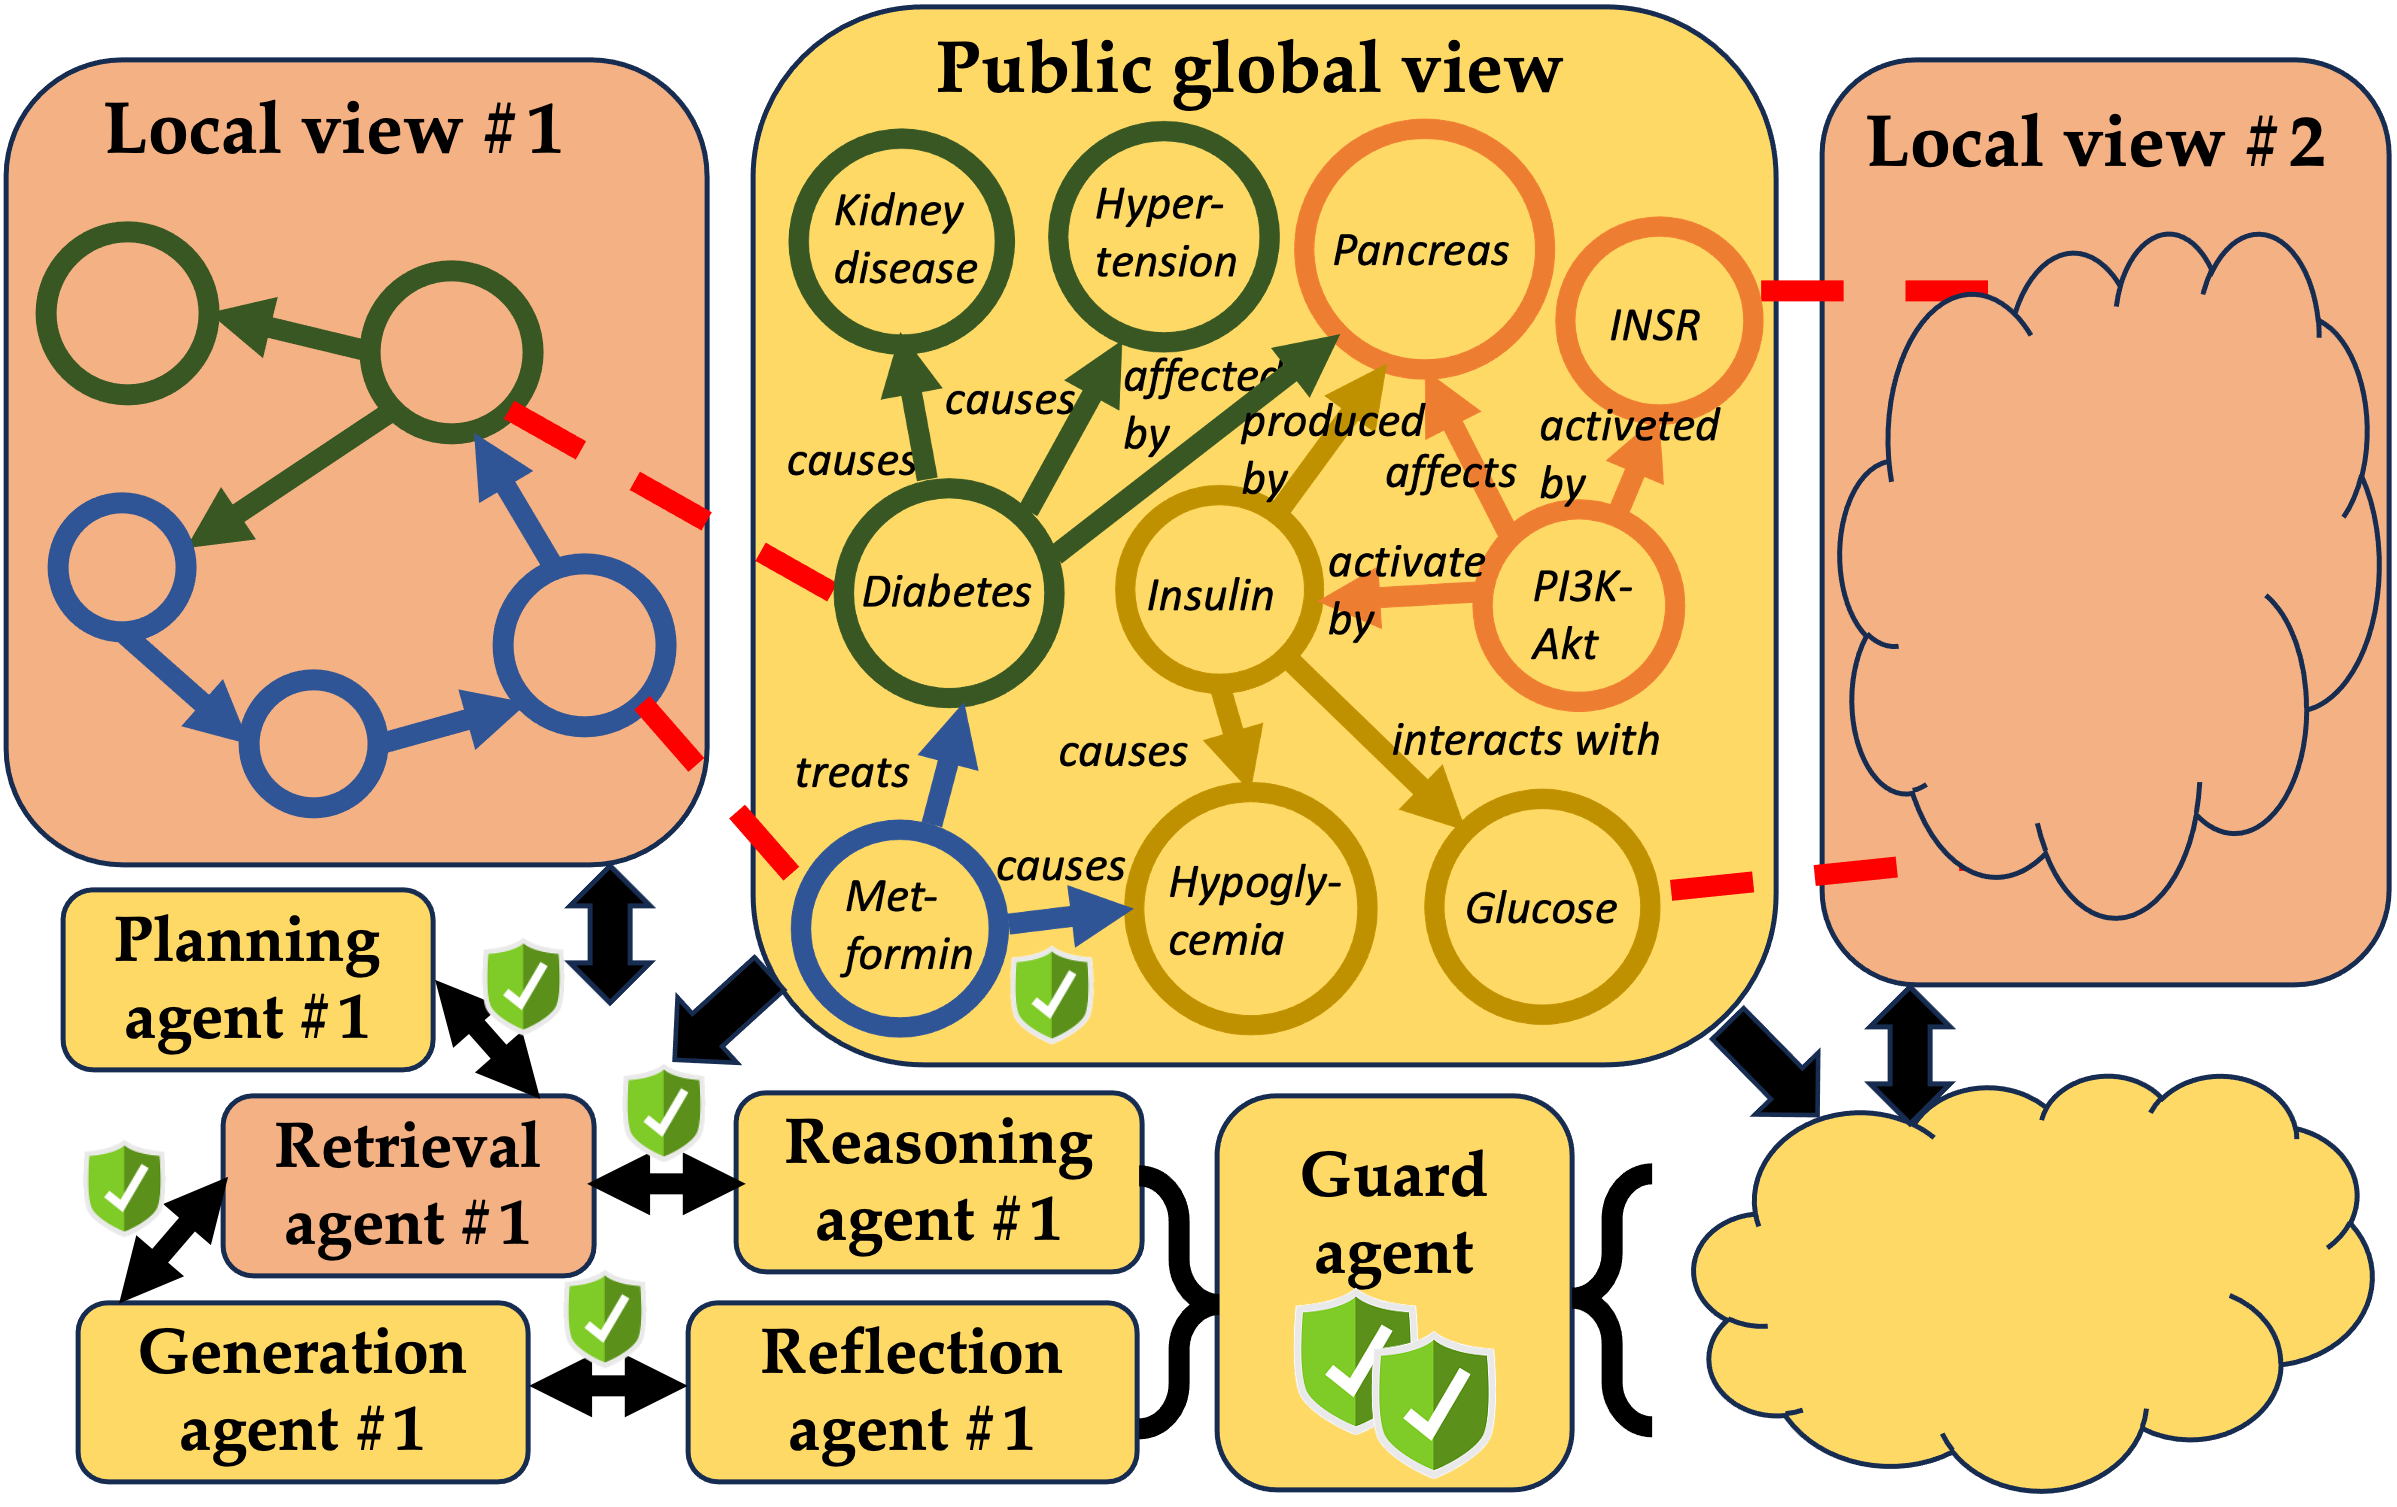
\includegraphics[width=.75\columnwidth]{submissions/CarlYang2024/figures/fedmas.png}
    \end{center}
    % \vspace{-3mm}
    \caption{The envisioned framework of a federated multi-agent system (FedMAS).}
    \label{fig:fedmas}
    % \vspace{-5mm}
\end{figure}

As illustrated in Figure \ref{fig:fedmas}, our envisioned FedMAS will include a multi-view KG and various LLM agents. The federation on KG will be implemented by collectively constructing a multi-view KG by all participating sites, where knowledge from public resources is integrated into the global view, and knowledge from private resources is kept in each site's local view only visible to itself. For each site, entities in its local view are linked with the global view, and only the embeddings related to these linked entities are shared with the server and other sites, via privacy-guaranteed embedding sharing algorithms such as those developed in FedDEP \cite{zhang2024deep} and FedR \cite{zhang2022efficient}. In this way, each local site can compute embeddings on its local view and the public view as if they can see all other sites' local views, allowing them to effectively adjust their local knowledge and further enhance their local LLMs, all without actually seeing the other sites' local views (knowledge). The server will periodically adjust knowledge in the global view also based on the shared privacy-guaranteed embeddings, and apply additional privacy checks to make sure no sensitive knowledge gets propagated into the global view.
%potentially discussing why knowledge is less private and how to avoid inference attack on embeddings

To rigorously protect the more sensitive patient data during the federation on LLM, it is possible to train multiple LLM agents in each site with different functions and let them collaborate through conversations instead of traditional model sharing, so the system can strictly control the level of private data each agent can access and monitor or moderate their collaborations. 
%Based on this design of multi-view KG, we will further enable the federation on LLM by training multiple LLM agents in each site and let them collaborate inside and across sites through conversations. 
%To control the levels of private data access and facilitate the moderation of conversations, each site will train multiple LLM agents focusing on different functions such as planning, retrieval, reasoning, reflection and answer generation. Since all agents will access certain levels of local private data during training and inference, none of them can be directly trained across sites even through FL. To this end, we will build on AutoGen \cite{} to design a structured conversational environment for multi-agent collaboration of LLMs. 
Specifically, since the retrieval agents need to access all local patient data, one plan is to implement programmable guardrails \cite{rebedea2023nemo} on its conversations with all other agents within the same site and forbid them from directly communicating with agents from other sites. Since all other agents can only access patient data indirectly through the retrieval agents, it is possible to adapt techniques such as our recently developed GuardAgent \cite{xiang2024guardagent} based on the clear goals and typical outputs of each agent to monitor all cross-site conversations, detecting and removing any suspicious private information.
%Specifically, since the retrieval and generation agents can directly access local patient data, we will only enable strict one-way conversations from other agents to them; since the planning, reasoning and reflection agents only access local KGs and their performances can likely benefit from cross-site collaborations (such as due to richer knowledge access and more generalized capabilities), we will enable two-way conversations among them cross sites; when the system is normal, we do not expect the agents to ask or answer privacy sensitive questions, and since each agent has clear goals, it will also be relatively easy to detect abnormal conversations; we will also explore techniques such as DP-prompting \cite{} to moderate the conversations against privacy leakage, and conduct red teaming \cite{} to rigorously monitor the conversations.  

When applying FedMAS to specific application domains such as finance, law, education, and healthcare, it is promising to leverage the knowledge-based data sharing mechanism to incorporate existing domain knowledge towards further alleviating knowledge gaps and mitigating potential biases. 
Built on recent promising results from LLM-based data annotations as discussed in Section 2, FedMAS can utilize specialized LLM agents to perform comprehensive extraction of structured knowledge from existing guidelines and tutorials and automatically integrate them with existing general and domain-specific KGs. For example, in healthcare, one type of important domain-specific entity is social determinants of health (SDOH) \cite{artiga2020disparities, artiga2018beyond, who2008closing}. The system can start with a set of known SDOH such as defined by WHO \cite{marmot2005social, phelan2010social}, and further extend the set and discover their impacts and relationships with various risk factors by investigating relevant healthcare literature. The KGs enhanced through these steps are supposed to facilitate the alleviation of various health disparities when utilized by subsequent LLM agents in the FedMAS. 
%Specifically, we will (1) adapt techniques in Thrust 1 with a focus on identifying SDOH-related entities and relations, such as by using the key factors in Figure \ref{fig:t3-3} to create an initial SDOH ontology and using LLMs for its further expansion to include more fine-grained factors; (2) conduct controlled experiments by finding and synthesizing pairs of patient data which only differ by certain SDOH factors, and analyzing LLM outputs for them regarding different clinical questions; (3) based on insights from (2), design programmable guardrails \cite{rebedea2023nemo} to enforce LLMs to output SDOH-removed predictions for tasks such as disease diagnosis where fairness is concerned, and output SDOH-informed predictions for tasks such as treatment suggestion where patients' financial abilities and access to healthcare resources should be considered.

While FedMAS utilizes AI advances to automate multi-site data integration and modeling, comprehensive and trustworthy AI systems need to also incorporate the values and needs of various stakeholders, who can have different and even contradictory perspectives. LLMs, especially in our multi-agent conversational environment, provide unique convenience for effective and efficient human participation, where different stakeholders can verify, influence, and complement the decision processes and outputs of different LLM agents, all based on natural languages as the interface.
Specifically, we envision a novel multi-stage intervention mechanism to efficiently enable the participation of different stakeholders in the LLM-based multi-agent conversational environment. The potential stages could include (1) LLM uncertainty quantification, where LLMs highlight their own uncertain outputs; (2) Rubrics-based rating, where humans create rubrics to automatically rate the LLM outputs; (3) Focused human interactions, where humans directly interact with LLMs, focusing on the problematic scenarios identified in the previous stages. The overall multi-stage mechanism is supposed to allow FedMAS to adapt to human values through iteratively integrating the language-based feedback via interactions with various stakeholders. 

%Instead of having the stakeholders freely chat with LLM agents, the mechanism will work as follows: Stage-1 (Uncertainty): LLM uncertainty quantification methods \cite{farquhar2024detecting, lu2024uncertainty} will be performed to identify potentially problematic answers such as due to hallucinations or data biases; Stage-2 (Rubrics): Rubrics manually generated from stakeholder feedback on a small development set such as based on the guidelines in Figure \ref{fig:t3-2} will be applied to automatically rate new LLM outputs, further exploring or highlighting problematic answers. Stage-3 (Human): Limited and costly human interactions will focus on problematic LLM outputs detected through the previous stages; %, either (partially) following the feedback guidelines or through free-form conversations; the stakeholders will also participate in elaborated surveys after interactions with LLMs, to summarize thoughts and concerns. On a development set, we will have the three stages cross-validate each other to evaluate their individual effectiveness and uncover potentially missed problematic LLM outputs in each individual stage. The uncertainty measurements, rubrics and feedback guidelines will be revised iteratively after the stakeholder surveys and cross-stage validations.

\section{Conclusions and Future Directions}
% \carl{Shirui, can you start helping with this section?}

In this paper, we discuss the trending efforts of co-learning KGs and LLMs. Through the lens of SRAG, we showcase promising attempts to utilize LLMs to automate the construction, integration, and enrichment of KGs, and discuss how KGs can help with planning paths, guide reasoning with structure, and ground knowledge with reflection, enhancing the reliability of LLMs for downstream tasks. We also envision a novel system of multiple agents collaborating in a conversational federated learning environment based on the knowledge-infused, human-engaged LLMs. While the co-learning of KGs and LLMs holds great potential, we envision several promising directions especially from the SRAG perspective.

\paragraph{Effective evaluation of LLM-generated knowledge.}
To achieve effective knowledge enrichment for KGs with LLMs, it is critical to evaluate and guarantee the quality of added and/or modified knowledge. However, new knowledge is hard to evaluate in nature due to the lack of ground truth. Exhaustive human evaluation is costly, but LLMs can be utilized to lubricate the collaboration between humans and machines toward efficient new knowledge evaluation. For example, humans can create guidelines and rubrics for LLMs to screen and rate the new knowledge from different perspectives. LLMs can also evaluate the quality of knowledge with confidence or uncertainty quantifications. Humans can then focus on the LLM-flagged suspicious or uncertain new knowledge to conduct close manual evaluation. 

\paragraph{Unified versus specialized KGs.}
Due to the diversity and breadth of knowledge, it might be difficult to integrate all knowledge into a single unified KG, which might potentially harm the knowledge integrity. As a potential alternative, it may become practical to construct specialized KGs depending on the knowledge needs of different applications. It then remains an open problem regarding how to measure the relevance of knowledge with respect to specific applications and decide what to include/exclude from the specialized KGs.

\paragraph{More powerful KGs.}
Current KGs mostly include general, binary, and pair-wise relations. However, when KGs are used in certain applications, the knowledge may not equally hold for every context. For example, one drug may treat a disease for only certain groups of patients. In such scenarios, specific mechanisms are needed to model the various contexts for knowledge. Moreover, relations are not always binary and pair-wise (between pairs of entities). They can be true with a probability and involve more than two entities. Such scenarios are ubiquitous in reality, so probabilistic KGs and n-ary KGs should receive wider adoption and study.


\paragraph{Trade-off between effectiveness and efficiency of retrieval.}
Most existing retrieval-based methods focus on developing an effective retrieval mechanism to accurately retrieve relevant knowledge from KGs \cite{li2023graph,yang2024kg}. However, they often overlook the efficiency of the retrieval process. In practice, the retrieval process can be computationally expensive, especially when the KG is large. Meanwhile, real-world application often requires prompt responses, which further exacerbates the efficiency issue. Therefore, it is essential to strike a balance between the effectiveness and efficiency of the retrieval process \cite{dehghan-etal-2024-ewek}.

\paragraph{Resolving knowledge conflicts (internal LLM knowledge versus external knowledge).}
LLMs contain a vast amount of knowledge obtained via pre-training. However, the knowledge might be inaccurate or outdated, which could conflict with the knowledge retrieved from KGs \cite{xu2024knowledge}. To resolve the conflict, SPARE \cite{zhao2024steering} utilizes the internal activations of LLMs to identify the conflict. AstuteRAG \cite{wang2024astute} uses a novel RAG approach to adaptively elicit LLM internal knowledge and iteratively consolidate internal and external knowledge. Despite the attempts, how to effectively identify and resolve the conflict between the internal knowledge of LLMs and the external knowledge retrieved from KGs remains an open problem.

\paragraph{Retrieval from multi-modal data.}
KGs store knowledge in diverse modalities such as text, image, and video \cite{zhu2022multi}. Existing KG retrieval methods mainly focus on retrieving textual knowledge. However, the retrieval from multi-modal data is still under-explored. Knowledge from different modalities can complement each other, which could potentially enhance the retrieval performance. Therefore, it is essential to develop retrieval methods that can effectively retrieve knowledge from multi-modal data \cite{long2024generative}.

\paragraph{Robustness/safety of SRAG for LLMs.} 
The safety and robustness of LLMs are receiving increasing attention due to their critical role in developing trustworthy AI systems. Previous research has primarily focused on attacking the LLMs themselves \cite{kumar2023certifying}. However, integrating LLMs with KG retrieval systems expands the attack surface. Attackers could manipulate KGs and the retrieval systems to mislead LLMs, potentially leading to severe consequences \cite{cheng2024trojanrag}. Therefore, enhancing the robustness and safety of the combined KG and LLM systems is an important research direction.

%The attack surface of KGs + LLMs system is enlarged compared with normal LLM systems. How to enhance the robustness and safety of these systems remains an open question \cite{li2024robustness}.
% The attack surface of KGs + LLMs system is enlarged compared with normal LLM systems. How to enhance the robustness and safety of these systems?



\section*{Acknowledgements}
This research was partially supported by the National Science Foundation under Award Number 2319449 and Award Number 2312502, as well as the National Institute Of Diabetes And Digestive And Kidney Diseases of the National Institutes of Health under Award Number K25DK135913. Any opinions, findings, and conclusions or recommendations expressed herein are those of the authors and do not necessarily represent the views, either expressed or implied, of the National Science Foundation, National Institutes of Health, or the U.S. government.
The authors wish to thank the editors and reviewers for their valuable efforts and suggestions.  

%% \ackrule

\bibliographystyle{IEEEtran} 
\bibliography{submissions/CarlYang2024/carlyang,submissions/CarlYang2024/linhao}

%\section*{Biographies}

%\textbf{P. W. Wachulak} received the degree${\ldots}$ \\[6pt]
%\textbf{M. C. Marconi} received the degree${\ldots}$ \\[6pt]
%\textbf{R. A. Bartels} received the degree${\ldots}$ \\[6pt]
%\textbf{C. S. Menoni} received the degree${\ldots}$ \\[6pt]
%\textbf{J. J. Rocca} received the degree${\ldots}$



\end{document}
\end{article}

\begin{article}
{Retrieval Augmented Generation in the Wild: A \emph{System 2} Perspective}
{Sajjadur Rahman, Dan Zhang, Nikita Bhutani, Estevam Hruschka, Eser Kandogan}
\setcounter{section}{0}
\pdfminorversion=5
\documentclass[11pt]{article}
\usepackage{deauthor,times,graphicx,caption,microtype}
\usepackage{hyperref}
\usepackage{listings}
\usepackage{booktabs}

\begin{document}

\title{Optimistic Lock Coupling: A Scalable and Efficient General-Purpose Synchronization Method}

\author{Viktor Leis, Michael Haubenschild\raisebox{0.9ex}{$\ast$}, Thomas Neumann\\ Technische Universit{\"a}t M{\"u}nchen \hspace{0.7cm} Tableau Software\raisebox{0.9ex}{$\ast$} \\ {\{leis,neumann\}{@}in.tum.de} \hspace{0.7cm} {mhaubenschild{@}tableau.com\raisebox{0.9ex}{$\ast$}}}

\maketitle

\begin{abstract}
As the number of cores on commodity processors continues to increase, scalability becomes more and more crucial for overall performance.
Scalable and efficient concurrent data structures are particularly important, as these are often the building blocks of parallel algorithms.
Unfortunately, traditional synchronization techniques based on fine-grained locking have been shown to be unscalable on modern multi-core CPUs.
Lock-free data structures, on the other hand, are extremely difficult to design and often incur significant overhead.

In this work, we make the case for Optimistic Lock Coupling as a practical alternative to both traditional locking and the lock-free approach.
We show that Optimistic Lock Coupling is highly scalable and almost as simple to implement as traditional lock coupling.
Another important advantage is that it is easily applicable to most tree-like data structures.
We therefore argue that Optimistic Lock Coupling, rather than a complex and error-prone custom synchronization protocol, should be the default choice for performance-critical data structures.
\end{abstract}

\section{Introduction}

% more and more cores
Today, Intel's commodity server processors have up to 28 cores and its upcoming microarchitecture will have up to 48 cores per socket~\cite{intel}.
Similarly, AMD currently stands at 32 cores and this number is expected to double in the next generation~\cite{amd}.
Since both platforms support simultaneous multithreading (also known as hyperthreading), affordable commodity servers (with up to two sockets) will soon routinely have between 100 and 200 hardware threads.

% data structure scalability is important
With such a high degree of hardware parallelism, efficient data processing crucially depends on how well concurrent data structures scale.
Internally, database systems use a plethora of data structures like table heaps, internal work queues, and, most importantly, index structures.
Any of these can easily become a scalability (and therefore overall performance) bottleneck on many-core CPUs.

% traditional synchronization: fine-grained locks, slow, cache invalidation
Traditionally, database systems synchronize internal data structures using fine-grained reader/writer locks\footnote{In this work, we focus on data structure synchronization rather than high-level transaction semantics and therefore use the term {\em lock} for what would typically be called {\em latch} in the database literature. We thus follow common computer science (rather than database) terminology.}.
Unfortunately, while fine-grained locking makes lock contention unlikely, it still results in bad scalability because lock acquisition and release require writing to shared memory.
Due to the way cache coherency is implemented on modern multi-core CPUs, these writes cause additional cache misses\footnote{The cache coherency protocol ensures that all copies of a cache line on other cores are invalidated before the write can proceed.} and the cache line containing the lock's internal data becomes a point of physical contention.
As a result, any frequently-accessed lock (e.g., the lock of the root node of a B-tree) severely limits scalability.

% lock-free bw-tree: no more latches, but indirections, extremely complex
Lock-free data structures like the Bw-tree~\cite{DBLP:conf/icde/LevandoskiLS13a} (a lock-free B-tree variant) or the Split-Ordered List~\cite{DBLP:journals/jacm/ShalevS06} (a lock-free hash table) do not acquire any locks and therefore generally scale much better than locking-based approaches (in particular for read-mostly workloads).
However, lock-free synchronization has other downsides:
First, it is very difficult and results in extremely complex and error-prone code (when compared to locking).
Second, because the functionality of atomic primitives provided by the hardware (e.g., atomically compare-and-swap 8 bytes) is limited, complex operations require additional indirections within the data structure.
For example, the Bw-tree requires an indirection table and the Split-Ordered List requires ``dummy nodes'', resulting in overhead due to additional cache misses.

% OLC for the win
In this paper we make the case for {\em Optimistic Lock Coupling (OLC)}, a synchronization method that combines some of the best properties of lock-based and lock-free synchronization.
OLC utilizes a special lock type that can be used in two modes:
The first mode is similar to a traditional mutex and excludes other threads by physically acquiring the underlying lock.
In the second mode, reads can proceed optimistically by validating a version counter that is embedded in the lock (similar to optimistic concurrency control).
The first mode is typically used by writers and the second mode by readers.
Besides this special lock type, OLC is based on the observation that optimistic lock validations can be interleaved/coupled---similar to the pair-wise interleaved lock acquisition of traditional lock coupling.
Hence, the name Optimistic Lock Coupling.

OLC has a number of desirable features:
\begin{itemize}
\item By reducing the number of writes to shared memory locations and thereby avoiding cache invalidations, it {\bf scales well} for most workloads.
\item In comparison to unsynchronized code, it requires few additional CPU instructions making it {\bf efficient}.
\item OLC is {\bf widely applicable} to different data structures. It has already been successfully used for synchronizing binary search trees~\cite{DBLP:conf/ppopp/BronsonCCO10}, tries~\cite{artsync}, trie/B-tree hybrids~\cite{DBLP:dblp_conf/eurosys/MaoKM12}, and B-trees~\cite{buzzword}.
\item In comparison to the lock-free paradigm, it is also {\bf easy to use} and requires few modifications to existing, single-threaded data structures.
\end{itemize}
Despite these positive features and its simplicity, OLC is not yet widely known.
The goal of this paper is therefore to popularize this simple idea and to make a case for it.
We argue that OLC deserves to be widely known.
It is a good default synchronization paradigm---more complex, data structure-specific protocols are seldom beneficial.

The rest of the paper is organized as follows.
Section~\ref{sec:related} discusses related work, tracing the history of OLC and its underlying ideas in the literature.
The core of the paper is Section~\ref{sec:olc}, which describes the ideas behind OLC and how it can be used to synchronize complex data structures.
In Section~\ref{sec:evaluation} we experimentally show that OLC has low overhead and scales well when used to synchronize an in-memory B-tree.
We summarize the paper in Section~\ref{sec:conc}.

\newpage
\section{Related Work}\label{sec:related}

Lock coupling has been proposed as a method for allowing concurrent operations on B-trees in 1977~\cite{DBLP:journals/acta/BayerS77}.
This traditional and still widely-used method, described in detail in Graefe's B-tree survey~\cite{DBLP:journals/ftdb/Graefe11}, is also called ``latch coupling'', ``hand-over-hand locking'', and ``crabbing''.
Because at most two locks are held at-a-time during tree traversal, this technique seemingly allows for a high degree of parallelism---in particular if read/write locks are used to enable inner nodes to be locked in shared mode.
However, as we show in Section~\ref{sec:evaluation}, on modern hardware lock acquisition (even in shared mode) results in suboptimal scalability.

An early alternative from 1981 is a B-tree variant called B-link tree~\cite{DBLP:journals/tods/LehmanY81}, which only holds a single lock at a time.
It is based on the observation that between the release of the parent lock and the acquisition of the child lock, the only ``dangerous'' thing that could have happened is the split of a child node (assuming one does not implement merge operations).
Thus, when a split happens, the key being searched might end up on a neighboring node to the right of the current child node.
A B-link tree traversal therefore detects this condition and, if needed, transparently proceeds to the neighboring node.
Releasing the parent lock early is highly beneficial when the child node needs to be fetched from disk.
For in-memory workloads, however, the B-link tree has the same scalability issues as lock coupling (it acquires just as many locks).

The next major advance, Optimistic Latch-Free Index Traversal (OLFIT)~\cite{DBLP:conf/vldb/ChaHKK01}, was proposed in 2001.
OLFIT introduced the idea of a combined lock/update counter, which we call {\em optimistic lock}. % , for lack of a better name,
Based on these per-node optimistic locks and the synchronization protocol of the B-link tree, OLFIT finally achieves good scalability on parallel processors.
The OLFIT protocol is fairly complex, as it requires both the non-trivial B-link protocol and optimistic locks.
Furthermore, like the B-link tree protocol, it does not support merging nodes, and is specific to B-trees (cannot easily be applied to other data structures).

In the following two decades, the growth of main-memory capacity led to much research into other data structures besides the venerable B-tree.
Particularly relevant for our discussion is Bronson et al.'s~\cite{DBLP:conf/ppopp/BronsonCCO10} concurrent binary search tree, which is based on optimistic version validation and has a sophisticated, data structure-specific synchronization protocol.
To the best of our knowledge, this 2010 paper is the first that, as part of its protocol, interleaves version validation across nodes---rather than validating each node separately like OLFIT.
In that paper, this idea is called ``hand-over-hand, optimistic validation'', while we prefer the term Optimistic Lock Coupling to highlight the close resemblance to traditional lock coupling.
Similarly, Mao et al.'s~\cite{DBLP:dblp_conf/eurosys/MaoKM12} Masstree (a concurrent hybrid trie/B-tree) is also based on the same ideas, but again uses them as part of a more complex protocol.

The Adaptive Radix Tree (ART)~\cite{art} is another recent in-memory data structure, which we proposed in 2013.
In contrast to the two data structures just mentioned, it was originally designed with single-threaded performance in mind without supporting concurrency.
To add support for concurrency, we initially started designing a custom protocol called Read-Optimized Write Exclusion (ROWEX)~\cite{artsync}, which turned out to be non-trivial and requires modifications of the underlying data structure\footnote{Note that ROWEX is already easier to apply to existing data structures than the lock-free approach. The difficulty depends on the data structure. Applying ROWEX is hard for B-trees with sorted keys and fairly easy for copy-on-write data structures like the Height Optimized Trie~\cite{hot}---with ART being somewhere in the middle.}.
However, fairly late in the project, we also realized, that OLC {\em alone} (rather than as part of a more complex protocol) is sufficient to synchronize ART.
No other changes to the data structure were necessary.
Both approaches were published and experimentally evaluated in a followup paper~\cite{artsync}, which shows that, despite its simplicity, OLC is efficient, scalable, and generally outperforms ROWEX.

Similar results were recently published regarding B-trees~\cite{buzzword}.
In this experimental study a simple OLC-based synchronization outperformed the Bw-tree~\cite{DBLP:conf/icde/LevandoskiLS13a}, a complex lock-free synchronization approach.
Another recent paper shows that for write-intensive workloads, locking often performs better than lock-free synchronization~\cite{DBLP:conf/cidr/FaleiroA17}.
These experiences indicate that OLC is a general-purpose synchronization paradigm and motivate the current paper.

%foster b-tree\cite{DBLP:journals/tods/GraefeKK12}
%Shasha theory~\cite{DBLP:journals/tods/ShashaG88}

\section{Optimistic Lock Coupling}\label{sec:olc}

% locks suck
The standard technique for inter-thread synchronization is mutual exclusion using fine-grained locks.
In a B-tree, for example, every node usually has its own associated lock, which is acquired before accessing that node.
The problem of locking on modern multi- and many-core processors is that lock acquisition and release require writing to the shared memory location that implements the lock.
This write causes exclusive ownership of the underlying cache line and invalidates copies of it on all other processor cores.
For hierarchical, tree-like data structures, the lock of the root node becomes a point of physical contention---even in read-only workloads and even when read/write locks are used.
Depending on the specific data structure, number of cores, cache coherency protocol implementation, cache topology, whether Non-Uniform Memory Access (NUMA) is used, locking can even result in multi-threaded performance that is worse than single-threaded execution.

% in b-trees this happens very much
The inherent pessimism of locking is particularly unfortunate for B-trees:
Despite the fact that logical modifications of the root node are very infrequent, every B-tree operation must lock the root node during tree traversal\footnote{To a lesser extent this obviously applies to all inner nodes, not just the root.}.
Even the vast majority of update operations (with the exception of splits and merges), only modify a single leaf node.
These observations indicate that a more optimistic approach, which does not require locking inner nodes, would be very beneficial for B-trees.

\subsection{Optimistic Locks}

% optimism to the rescue
As the name indicates, optimistic locks try to solve the scalability issues of traditional locks using an optimistic approach.
Instead of always physically acquiring locks, even for nodes that are unlikely to be modified simultaneously, after-the-fact validation is used to detect conflicts.
This is done by augmenting each lock with a version/update counter that is incremented on every modification.
Using this version counter, readers can optimistically proceed before validating that the version did not change to ensure that the read was safe.
If validation fails, the operation is restarted.

% details on opt locks
Using optimistic locks, a read-only node access (i.e., the majority of all operations in a B-tree) does not acquire the lock and does not increment the version counter.
Instead, it performs the following steps:
\begin{enumerate}
\item read lock version (restart if lock is not free)
\item access node
\item read the version again and validate that it has not changed in the meantime
\end{enumerate}
If the last step (the validation) fails, the operation has to be restarted.
Write operations, on the other hand, are more similar to traditional locking:
\begin{enumerate}
\item acquire lock (wait if necessary)
\item access/write to node
\item increment version and unlock node
\end{enumerate}
Writes can therefore protect a node from other writes.

% similar to locks
As we observed in an earlier paper~\cite{artsync}, because of similar semantics, optimistic locks can be hidden behind an API very similar to traditional read/write locks.
Both approaches have an exclusive lock mode, and acquiring a traditional lock in shared mode is analogous to optimistic version validation.
Furthermore, like with some implementations of traditional read/write locks, optimistic locks allow upgrading a shared lock to an exclusive lock.
Lock upgrades are, for example, used to avoid most B-tree update operations from having to lock inner nodes.
In our experience, the close resemblance of optimistic and traditional locks simplifies the reasoning about optimistic locks;
one can apply similar thinking as in traditional lock-based protocols.

\subsection{Lock Coupling with Optimistic Locks}

\begin{figure}
  \centering
  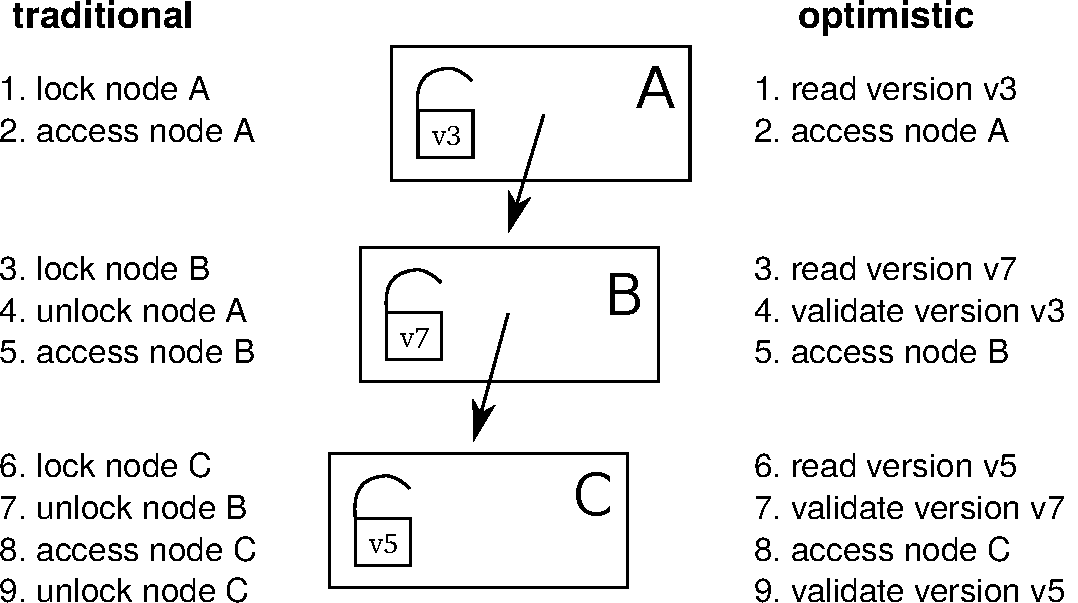
\includegraphics[width=0.65\linewidth]{olcall.pdf}
  \vspace{0.2cm}
  \caption{Comparison of a lookup operation in a 3-level tree using traditional lock coupling (left-hand side) vs.~optimistic lock coupling (right-hand side).}
  \label{fig:olc}
\end{figure}

The traditional and most common lock-based synchronization protocol for B-trees is lock coupling, which interleaves lock acquisitions while holding at most two locks at a time.
If, as we observed earlier, optimistic locks have similar semantics as traditional locks, it is natural to ask whether lock coupling can be combined with optimistic locks.
And indeed the answer is yes: One can almost mechanically translate traditional lock coupling code to optimistic lock coupling code.
This is illustrated in Figure~\ref{fig:olc}, which compares the traversal in a tree of height 3 using traditional and optimistic locks.
As the figure shows, the main difference is that locking is translated to reading the version and that unlocking becomes validation of the previously read version.
This simple change provides efficient lock-free tree traversal without the need to design a complex synchronization protocol.

It is important to emphasize the conceptual simplicity of OLC in comparison to data structures that use custom protocols like the Bw-tree~\cite{DBLP:conf/icde/LevandoskiLS13a}.
To implement lock-free access, the Bw-tree requires an indirection table, delta nodes, complex splitting and merging logic, retry logic, etc.
OLC, on the other hand, can directly be applied to B-trees mostly by adding the appropriate optimistic locking code and without modifying the node layout itself.
Therefore, OpenBw-Tree, an open source implementation of the Bw-tree, requires an order of magnitude more code than a B-tree based on OLC\footnote{Both implementations are available on GitHub: \url{https://github.com/wangziqi2016/index-microbench}}.
Given how difficult it is to develop, validate, and debug lock-free code, simplicity is obviously a major advantage.

\subsection{Correctness Aspects}

\begin{figure}
  % \centering
  %[basicstyle=\normalsize\ttfamily,showstringspaces=false,columns=fullflexible,breaklines=false,breakatwhitespace=true,numbers=none,numberstyle=\small,style=C,keepspaces=true]
\begin{lstlisting}[basicstyle=\ttfamily,language=C++,numbers=left,numberstyle=\small]
std::atomic<BTreeNode*> root;

// search for key in B+tree, returns payload in resultOut
bool lookup(Key key, Value& resultOut) {
   BTreeNode* node = root.load();
   uint64_t nodeVersion = node->readLockOrRestart();
   if (node != root.load()) // make sure the root is still the root
      restart();

   BTreeInner<Key>* parent = nullptr;
   uint64_t parentVersion = 0;

   while (node->isInner()) {
      auto inner = (BTreeInner*)node;

      // unlock parent and make current node the parent
      if (parent)
         parent->readUnlockOrRestart(parentVersion);
      parent = inner;
      parentVersion = nodeVersion;

      // search for next node
      node = inner->findChild(key);
      // validate 'inner' to ensure that 'node' pointer is valid
      inner->checkOrRestart(nodeVersion);
      // now it safe to dereference 'node' pointer (read its version)
      nodeVersion = node->readLockOrRestart();
   }

   // search in leaf and retrieve payload
   auto leaf = (BTreeLeaf*)node;
   bool success = leaf->findValue(key, resultOut);

   // unlock everything
   if (parent)
      parent->readUnlockOrRestart(parentVersion);
   node->readUnlockOrRestart(nodeVersion);

   return success;
}
\end{lstlisting}
  \vspace{0.2cm}
  \caption{B-tree lookup code using OLC. For simplicity, the restart logic is not shown.}
  \label{fig:lookup}
\end{figure}

So far, we have introduced the high-level ideas behind OLC and have stressed its similarity to traditional lock coupling.
Let us now discuss some cases where the close similarity between lock coupling and OLC breaks down.
To make this more concrete, we show the B-tree lookup code in Figure~\ref{fig:lookup}.
In the code, \texttt{readLockOrRestart} reads the lock version and \texttt{readUnlockOrRestart} validates that the read was correct.

One issue with OLC is that any pointer speculatively read from a node may point to invalid memory (if that node is modified concurrently).
Dereferencing such a pointer (e.g., to read its optimistic lock), may cause a segmentation fault or undefined behavior.
In the code shown in Figure~\ref{fig:lookup}, this problem is prevented by the extra check in line 25, which ensures that the read from the node containing the pointer was correct.
Without this additional validation, the code would in line 27 dereference the pointer speculatively read in line 23.
Note that the implementation of \texttt{checkOrRestart} is actually identical to \texttt{readUnlockOrRestart}.
We chose to give it a different name to highlight the fact that this extra check would not be necessary with read/write locks.

Another potential issue with optimistic locks is code that does not terminate.
Code that speculatively accesses a node, like an intra-node binary search, should be written in a way such that it always terminates---even in the presence of concurrent writes.
Otherwise, the validation code that detects the concurrent write will never run.
The binary search of a B-tree, for example, needs to be written in such a way that each comparison makes progress.
For some data structures that do not require loops in the traversal code (like ART) termination is trivially true.

\subsection{Implementation Details}

% implementation, efficiency
To implement an optimistic lock, one can combine the lock and the version counter into a single 64-bit\footnote{Even after subtracting one bit for the lock status, a back-of-the-envelope calculation can show that 63 bits are large enough to never overflow in practice.} word~\cite{artsync}.
A typical read operation will therefore merely consist of reading this version counter atomically.
In C++11 this can be implemented using the \texttt{std::atomic} type.

On x86, atomic reads are cheap because of x86's strong memory order guarantees.
No memory fences are required for sequentially-consistent loads, which are translated (by both GCC and clang) into standard \texttt{MOV} instructions.
Hence, the only effect of \texttt{std::atomic} for loads is preventing instruction re-ordering.
This makes version access and validation cheap.
Acquiring and releasing an optimistic lock in exclusive mode has comparable cost to a traditional lock:
A fairly expensive sequentially-consistent store is needed for acquiring a lock, while a standard \texttt{MOV} suffices for releasing it.
A simple sinlock-based implementation of optimistic locks can be found in the appendix of an earlier paper~\cite{artsync}.

OLC code must be able to handle restarts since validation or lock upgrade can fail due to concurrent writers.
Restarts can easily be implemented by wrapping the data structure operation in a loop (for simplicity not shown in Figure~\ref{fig:lookup}).
Such a loop also enables limiting the number of optimistic retry operations and falling back to pessimistic locking in cases of very heavy contention.
The ability to fall back to traditional locking is a major advantage of OLC in terms of robustness over lock-free approaches, which do not have this option.

In addition to the optimistic shared mode and the exclusive mode, optimistic locks also support a ``shared pessimistic'' mode, which physically acquires the lock in shared mode (allowing multiple concurrent readers but no writers).
This mode is useful for table (or range) scans that touch many tuples on a leaf page (which would otherwise easily abort).
Finally, let us mention that large range scans and table scans, should be broken up into several per-node traversals as is done in the LeanStore~\cite{leanstore} system.

Like all lock-free data structures, but unlike traditional locking and Hardware Transactional Memory~\cite{DBLP:conf/hpca/KarnagelDRLLSL14,DBLP:journals/pvldb/MakreshanskiLS15,htmtkde}, OLC requires care when deleting (and reusing) nodes.
The reason is that a deleting thread can never be sure that a node can be reclaimed because other threads might still be optimistically reading from that node.
Therefore, standard solutions like epoch-based reclamation~\cite{DBLP:conf/sosp/TuZKLM13}, hazard pointers~\cite{DBLP:journals/tpds/Michael04}, or optimized hazard pointers~\cite{DBLP:conf/spaa/BalmauGHZ16} need to be used.
These memory reclamation techniques are, however, largely orthogonal to the synchronization protocol itself.

%-lock-free is not a strong guarantee

\newpage
\section{Evaluation}\label{sec:evaluation}

Let us now experimentally evaluate the overhead and scalability of OLC.
For the experiments, we use an in-memory B+tree implemented in C++11 using templates, which is configured to use nodes of 4096 bytes, random 8 byte keys, and 8 byte payloads.
Based on this B-tree, we compare the following synchronization approaches:
\begin{itemize}
\item an OLC implementation\footnote{An almost identical OLC implementation is available on github: \url{https://github.com/wangziqi2016/index-microbench/tree/master/BTreeOLC}}
\item a variant based on traditional lock coupling and read/write locks
\item the unsynchronized B-tree, which obviously is only correct for read-only workloads but allows measuring the overhead of synchronization
\end{itemize}
Note that earlier work has compared the OLC implementation with a Bw-tree implementation~\cite{buzzword} and other state-of-the-art in-memory index structures.

We use a Haswell EP system with an Intel Xeon E5-2687W v3 CPU, which has 10 cores (20 ``Hyper-Threads'') and 25~MB of L3 cache.
The system is running Ubuntu 18.10 and we use GCC 8.2.0 to compile our code.
The CPU counters are obtained using the Linux perf API\footnote{We use the following convenience wrapper: \url{https://github.com/viktorleis/perfevent}}.

\begin{table}
  \caption{Performance and CPU counters for lookup and insert operations in a B-tree with 100M keys. We perform 100M operations and normalize the CPU counters by that number.}
  \label{tab:overhead}
  \centering
  \begin{tabular}{lrrrrrrr}\toprule
                    &         &        &        & instruc-  & L1     & L3     & branch \\
                    & threads & M op/s & cycles & tions & misses & misses & misses \\\midrule
lookup (no sync.)   & 1       & 1.72   & 2028   & 283     & 39.1   & 14.9   & 16.1   \\
lookup (OLC)        & 1       & 1.65   & 2107   & 370     & 43.9   & 15.1   & 16.7   \\
lookup (lock coup.) & 1       & 1.72   & 2078   & 365     & 42.3   & 16.9   & 15.7   \\\midrule
insert (no sync.)   & 1       & 1.51   & 2286   & 530     & 59.8   & 31.1   & 17.3   \\
insert (OLC)        & 1       & 1.50   & 2303   & 629     & 61.2   & 31.1   & 16.5   \\
insert (lock coup.) & 1       & 1.41   & 2473   & 644     & 61.0   & 31.0   & 17.2   \\\midrule
lookup (no sync.)   & 10      & 15.48  & 2058   & 283     & 38.6   & 15.5   & 16.0   \\
lookup (OLC)        & 10      & 14.60  & 2187   & 370     & 43.8   & 15.8   & 16.8   \\
lookup (lock coup.) & 10      & 5.71   & 5591   & 379     & 54.2   & 17.0   & 14.8   \\\midrule
insert (no sync.)   & 10      & -      & -      & -       & -      & -      & -      \\
insert (OLC)        & 10      & 10.46  & 2940   & 656     & 62.0   & 32.5   & 16.8   \\
insert (lock coup.) & 10      & 7.55   & 4161   & 667     & 75.0   & 28.6   & 16.2   \\
    \bottomrule
\end{tabular}
\end{table}

Table~\ref{tab:overhead} compares the performance and CPU counters for lookup and insert operations in a B-tree with 100M keys.
With {\em single-threaded} execution, we observe that all three approaches have very similar performance.
Adding traditional or optimistic locks to unsynchronized B-tree code results in up to 30\% of additional instructions without affecting single-threaded performance much.

\begin{figure}
  \centering
  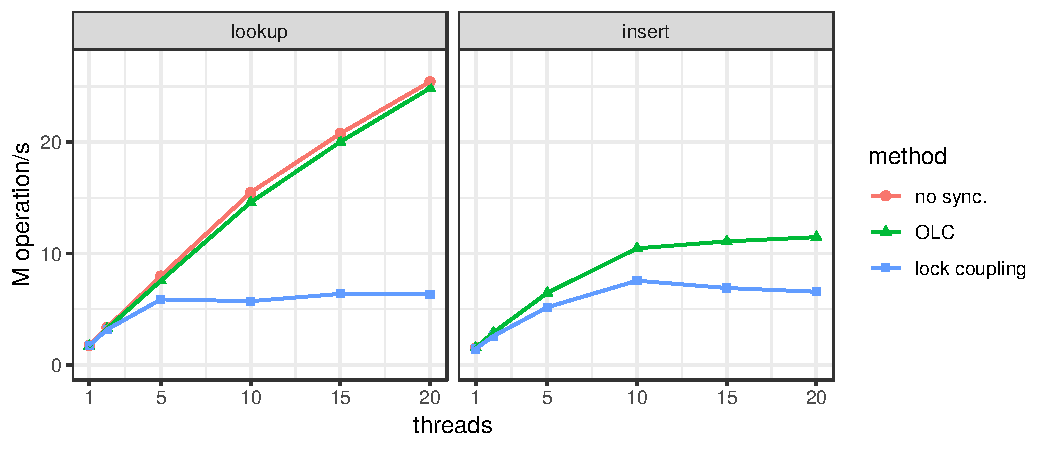
\includegraphics[width=\linewidth]{scale.pdf}
  \vspace{0.2cm}
  \caption{Scalability on 10-core system for B-tree operations (100M values).}
  \label{fig:scale}
\end{figure}

As Figure~\ref{fig:scale} shows, the results change dramatically once we use multiple threads.
For lookup, the scalability of OLC is near-linear up to 20 threads, even though the system has only 10 ``real cores''.
The OLC scalability for insert is also respectable (though not quite as linear because multi-threaded insertion approaches the memory bandwidth of our processor).
The figure also shows that the results of traditional lock coupling with read/write locks are significantly worse than OLC.
With 20 threads, lookup with OLC is 3.9$\times$ faster than traditional lock coupling.

\section{Summary}\label{sec:conc}

Optimistic Lock Coupling (OLC) is an effective synchronization method that combines the simplicity of traditional lock coupling with the superior scalability of lock-free approaches.
OLC is widely applicable and has already been successfully used to synchronize several data structures, including B-trees, binary search trees, and different trie variants.
These features make it highly attractive for modern database systems as well as performance-critical systems software in general.

\begin{thebibliography}{10}

\bibitem{DBLP:conf/spaa/BalmauGHZ16}
O.~Balmau, R.~Guerraoui, M.~Herlihy, and I.~Zablotchi.
\newblock Fast and robust memory reclamation for concurrent data structures.
\newblock In {\em SPAA}, 2016.

\bibitem{DBLP:journals/acta/BayerS77}
R.~Bayer and M.~Schkolnick.
\newblock Concurrency of operations on {B}-trees.
\newblock {\em Acta Informatica}, 9, 1977.

\bibitem{hot}
R.~Binna, E.~Zangerle, M.~Pichl, G.~Specht, and V.~Leis.
\newblock {HOT}: A height optimized trie index for main-memory database
  systems.
\newblock In {\em SIGMOD}, 2018.

\bibitem{DBLP:conf/ppopp/BronsonCCO10}
N.~G. Bronson, J.~Casper, H.~Chafi, and K.~Olukotun.
\newblock A practical concurrent binary search tree.
\newblock In {\em PPOPP}, 2010.

\bibitem{DBLP:conf/vldb/ChaHKK01}
S.~K. Cha, S.~Hwang, K.~Kim, and K.~Kwon.
\newblock Cache-conscious concurrency control of main-memory indexes on
  shared-memory multiprocessor systems.
\newblock In {\em VLDB}, 2001.

\bibitem{intel}
I.~Cutress.
\newblock {Intel} goes for 48-cores: {Cascade-AP} with multi-chip package
  coming soon.
\newblock
  \url{https://www.anandtech.com/show/13535/intel-goes-for-48cores-cascade-ap},
  2018 (accessed January, 2019).

\bibitem{DBLP:conf/cidr/FaleiroA17}
J.~M. Faleiro and D.~J. Abadi.
\newblock Latch-free synchronization in database systems: Silver bullet or
  fool's gold?
\newblock In {\em CIDR}, 2017.

\bibitem{DBLP:journals/ftdb/Graefe11}
G.~Graefe.
\newblock Modern {B}-tree techniques.
\newblock {\em Foundations and Trends in Databases}, 3(4), 2011.

\bibitem{DBLP:conf/hpca/KarnagelDRLLSL14}
T.~Karnagel, R.~Dementiev, R.~Rajwar, K.~Lai, T.~Legler, B.~Schlegel, and
  W.~Lehner.
\newblock Improving in-memory database index performance with
  {Intel}\({}^{\mbox{{\textregistered}}}\) transactional synchronization
  extensions.
\newblock In {\em HPCA}, 2014.

\bibitem{DBLP:journals/tods/LehmanY81}
P.~L. Lehman and S.~B. Yao.
\newblock Efficient locking for concurrent operations on {B}-trees.
\newblock {\em {ACM} Trans. Database Syst.}, 6(4), 1981.

\bibitem{leanstore}
V.~Leis, M.~Haubenschild, A.~Kemper, and T.~Neumann.
\newblock Leanstore: In-memory data management beyond main memory.
\newblock In {\em ICDE}, 2018.

\bibitem{art}
V.~Leis, A.~Kemper, and T.~Neumann.
\newblock The adaptive radix tree: {ARTful} indexing for main-memory databases.
\newblock In {\em ICDE}, 2013.

\bibitem{htmtkde}
V.~Leis, A.~Kemper, and T.~Neumann.
\newblock Scaling {HTM}-supported database transactions to many cores.
\newblock {\em {IEEE} Trans. Knowl. Data Eng.}, 28(2), 2016.

\bibitem{artsync}
V.~Leis, F.~Scheibner, A.~Kemper, and T.~Neumann.
\newblock The {ART} of practical synchronization.
\newblock In {\em DaMoN}, 2016.

\bibitem{DBLP:conf/icde/LevandoskiLS13a}
J.~J. Levandoski, D.~B. Lomet, and S.~Sengupta.
\newblock The {Bw}-tree: A {B}-tree for new hardware platforms.
\newblock In {\em ICDE}, 2013.

\bibitem{DBLP:journals/pvldb/MakreshanskiLS15}
D.~Makreshanski, J.~J. Levandoski, and R.~Stutsman.
\newblock To lock, swap, or elide: On the interplay of hardware transactional
  memory and lock-free indexing.
\newblock {\em {PVLDB}}, 8(11), 2015.

\bibitem{DBLP:dblp_conf/eurosys/MaoKM12}
Y.~Mao, E.~Kohler, and R.~T. Morris.
\newblock Cache craftiness for fast multicore key-value storage.
\newblock In {\em EuroSys}, 2012.

\bibitem{DBLP:journals/tpds/Michael04}
M.~M. Michael.
\newblock Hazard pointers: Safe memory reclamation for lock-free objects.
\newblock {\em {IEEE} Trans. Parallel Distrib. Syst.}, 15(6), 2004.

\bibitem{DBLP:journals/jacm/ShalevS06}
O.~Shalev and N.~Shavit.
\newblock Split-ordered lists: Lock-free extensible hash tables.
\newblock {\em J. {ACM}}, 53(3), 2006.

\bibitem{amd}
A.~Shilov.
\newblock {AMD} previews {EPYC} ‘{Rome}’ processor: Up to 64 {Zen} 2 cores.
\newblock
  \url{https://www.anandtech.com/show/13561/amd-previews-epyc-rome-processor-up-to-64-zen-2-cores},
  2018 (accessed January, 2019).

\bibitem{DBLP:conf/sosp/TuZKLM13}
S.~Tu, W.~Zheng, E.~Kohler, B.~Liskov, and S.~Madden.
\newblock Speedy transactions in multicore in-memory databases.
\newblock In {\em SOSP}, 2013.

\bibitem{buzzword}
Z.~Wang, A.~Pavlo, H.~Lim, V.~Leis, H.~Zhang, M.~Kaminsky, and D.~Andersen.
\newblock Building a {Bw}-tree takes more than just buzz words.
\newblock In {\em SIGMOD}, 2018.

\end{thebibliography}


%\bibliographystyle{abbrv}
%\bibliography{main}

\end{document}

\end{article}

\begin{article}
{RAG-based Question Answering over Heterogeneous Data and Text}
{Philipp Christmann, Gerhard Weikum}
\setcounter{section}{0}
\pdfminorversion=5
\documentclass[11pt]{article}
\usepackage{deauthor,times,graphicx,caption,microtype}
\usepackage{hyperref}
\usepackage{listings}
\usepackage{booktabs}

\begin{document}

\title{Optimistic Lock Coupling: A Scalable and Efficient General-Purpose Synchronization Method}

\author{Viktor Leis, Michael Haubenschild\raisebox{0.9ex}{$\ast$}, Thomas Neumann\\ Technische Universit{\"a}t M{\"u}nchen \hspace{0.7cm} Tableau Software\raisebox{0.9ex}{$\ast$} \\ {\{leis,neumann\}{@}in.tum.de} \hspace{0.7cm} {mhaubenschild{@}tableau.com\raisebox{0.9ex}{$\ast$}}}

\maketitle

\begin{abstract}
As the number of cores on commodity processors continues to increase, scalability becomes more and more crucial for overall performance.
Scalable and efficient concurrent data structures are particularly important, as these are often the building blocks of parallel algorithms.
Unfortunately, traditional synchronization techniques based on fine-grained locking have been shown to be unscalable on modern multi-core CPUs.
Lock-free data structures, on the other hand, are extremely difficult to design and often incur significant overhead.

In this work, we make the case for Optimistic Lock Coupling as a practical alternative to both traditional locking and the lock-free approach.
We show that Optimistic Lock Coupling is highly scalable and almost as simple to implement as traditional lock coupling.
Another important advantage is that it is easily applicable to most tree-like data structures.
We therefore argue that Optimistic Lock Coupling, rather than a complex and error-prone custom synchronization protocol, should be the default choice for performance-critical data structures.
\end{abstract}

\section{Introduction}

% more and more cores
Today, Intel's commodity server processors have up to 28 cores and its upcoming microarchitecture will have up to 48 cores per socket~\cite{intel}.
Similarly, AMD currently stands at 32 cores and this number is expected to double in the next generation~\cite{amd}.
Since both platforms support simultaneous multithreading (also known as hyperthreading), affordable commodity servers (with up to two sockets) will soon routinely have between 100 and 200 hardware threads.

% data structure scalability is important
With such a high degree of hardware parallelism, efficient data processing crucially depends on how well concurrent data structures scale.
Internally, database systems use a plethora of data structures like table heaps, internal work queues, and, most importantly, index structures.
Any of these can easily become a scalability (and therefore overall performance) bottleneck on many-core CPUs.

% traditional synchronization: fine-grained locks, slow, cache invalidation
Traditionally, database systems synchronize internal data structures using fine-grained reader/writer locks\footnote{In this work, we focus on data structure synchronization rather than high-level transaction semantics and therefore use the term {\em lock} for what would typically be called {\em latch} in the database literature. We thus follow common computer science (rather than database) terminology.}.
Unfortunately, while fine-grained locking makes lock contention unlikely, it still results in bad scalability because lock acquisition and release require writing to shared memory.
Due to the way cache coherency is implemented on modern multi-core CPUs, these writes cause additional cache misses\footnote{The cache coherency protocol ensures that all copies of a cache line on other cores are invalidated before the write can proceed.} and the cache line containing the lock's internal data becomes a point of physical contention.
As a result, any frequently-accessed lock (e.g., the lock of the root node of a B-tree) severely limits scalability.

% lock-free bw-tree: no more latches, but indirections, extremely complex
Lock-free data structures like the Bw-tree~\cite{DBLP:conf/icde/LevandoskiLS13a} (a lock-free B-tree variant) or the Split-Ordered List~\cite{DBLP:journals/jacm/ShalevS06} (a lock-free hash table) do not acquire any locks and therefore generally scale much better than locking-based approaches (in particular for read-mostly workloads).
However, lock-free synchronization has other downsides:
First, it is very difficult and results in extremely complex and error-prone code (when compared to locking).
Second, because the functionality of atomic primitives provided by the hardware (e.g., atomically compare-and-swap 8 bytes) is limited, complex operations require additional indirections within the data structure.
For example, the Bw-tree requires an indirection table and the Split-Ordered List requires ``dummy nodes'', resulting in overhead due to additional cache misses.

% OLC for the win
In this paper we make the case for {\em Optimistic Lock Coupling (OLC)}, a synchronization method that combines some of the best properties of lock-based and lock-free synchronization.
OLC utilizes a special lock type that can be used in two modes:
The first mode is similar to a traditional mutex and excludes other threads by physically acquiring the underlying lock.
In the second mode, reads can proceed optimistically by validating a version counter that is embedded in the lock (similar to optimistic concurrency control).
The first mode is typically used by writers and the second mode by readers.
Besides this special lock type, OLC is based on the observation that optimistic lock validations can be interleaved/coupled---similar to the pair-wise interleaved lock acquisition of traditional lock coupling.
Hence, the name Optimistic Lock Coupling.

OLC has a number of desirable features:
\begin{itemize}
\item By reducing the number of writes to shared memory locations and thereby avoiding cache invalidations, it {\bf scales well} for most workloads.
\item In comparison to unsynchronized code, it requires few additional CPU instructions making it {\bf efficient}.
\item OLC is {\bf widely applicable} to different data structures. It has already been successfully used for synchronizing binary search trees~\cite{DBLP:conf/ppopp/BronsonCCO10}, tries~\cite{artsync}, trie/B-tree hybrids~\cite{DBLP:dblp_conf/eurosys/MaoKM12}, and B-trees~\cite{buzzword}.
\item In comparison to the lock-free paradigm, it is also {\bf easy to use} and requires few modifications to existing, single-threaded data structures.
\end{itemize}
Despite these positive features and its simplicity, OLC is not yet widely known.
The goal of this paper is therefore to popularize this simple idea and to make a case for it.
We argue that OLC deserves to be widely known.
It is a good default synchronization paradigm---more complex, data structure-specific protocols are seldom beneficial.

The rest of the paper is organized as follows.
Section~\ref{sec:related} discusses related work, tracing the history of OLC and its underlying ideas in the literature.
The core of the paper is Section~\ref{sec:olc}, which describes the ideas behind OLC and how it can be used to synchronize complex data structures.
In Section~\ref{sec:evaluation} we experimentally show that OLC has low overhead and scales well when used to synchronize an in-memory B-tree.
We summarize the paper in Section~\ref{sec:conc}.

\newpage
\section{Related Work}\label{sec:related}

Lock coupling has been proposed as a method for allowing concurrent operations on B-trees in 1977~\cite{DBLP:journals/acta/BayerS77}.
This traditional and still widely-used method, described in detail in Graefe's B-tree survey~\cite{DBLP:journals/ftdb/Graefe11}, is also called ``latch coupling'', ``hand-over-hand locking'', and ``crabbing''.
Because at most two locks are held at-a-time during tree traversal, this technique seemingly allows for a high degree of parallelism---in particular if read/write locks are used to enable inner nodes to be locked in shared mode.
However, as we show in Section~\ref{sec:evaluation}, on modern hardware lock acquisition (even in shared mode) results in suboptimal scalability.

An early alternative from 1981 is a B-tree variant called B-link tree~\cite{DBLP:journals/tods/LehmanY81}, which only holds a single lock at a time.
It is based on the observation that between the release of the parent lock and the acquisition of the child lock, the only ``dangerous'' thing that could have happened is the split of a child node (assuming one does not implement merge operations).
Thus, when a split happens, the key being searched might end up on a neighboring node to the right of the current child node.
A B-link tree traversal therefore detects this condition and, if needed, transparently proceeds to the neighboring node.
Releasing the parent lock early is highly beneficial when the child node needs to be fetched from disk.
For in-memory workloads, however, the B-link tree has the same scalability issues as lock coupling (it acquires just as many locks).

The next major advance, Optimistic Latch-Free Index Traversal (OLFIT)~\cite{DBLP:conf/vldb/ChaHKK01}, was proposed in 2001.
OLFIT introduced the idea of a combined lock/update counter, which we call {\em optimistic lock}. % , for lack of a better name,
Based on these per-node optimistic locks and the synchronization protocol of the B-link tree, OLFIT finally achieves good scalability on parallel processors.
The OLFIT protocol is fairly complex, as it requires both the non-trivial B-link protocol and optimistic locks.
Furthermore, like the B-link tree protocol, it does not support merging nodes, and is specific to B-trees (cannot easily be applied to other data structures).

In the following two decades, the growth of main-memory capacity led to much research into other data structures besides the venerable B-tree.
Particularly relevant for our discussion is Bronson et al.'s~\cite{DBLP:conf/ppopp/BronsonCCO10} concurrent binary search tree, which is based on optimistic version validation and has a sophisticated, data structure-specific synchronization protocol.
To the best of our knowledge, this 2010 paper is the first that, as part of its protocol, interleaves version validation across nodes---rather than validating each node separately like OLFIT.
In that paper, this idea is called ``hand-over-hand, optimistic validation'', while we prefer the term Optimistic Lock Coupling to highlight the close resemblance to traditional lock coupling.
Similarly, Mao et al.'s~\cite{DBLP:dblp_conf/eurosys/MaoKM12} Masstree (a concurrent hybrid trie/B-tree) is also based on the same ideas, but again uses them as part of a more complex protocol.

The Adaptive Radix Tree (ART)~\cite{art} is another recent in-memory data structure, which we proposed in 2013.
In contrast to the two data structures just mentioned, it was originally designed with single-threaded performance in mind without supporting concurrency.
To add support for concurrency, we initially started designing a custom protocol called Read-Optimized Write Exclusion (ROWEX)~\cite{artsync}, which turned out to be non-trivial and requires modifications of the underlying data structure\footnote{Note that ROWEX is already easier to apply to existing data structures than the lock-free approach. The difficulty depends on the data structure. Applying ROWEX is hard for B-trees with sorted keys and fairly easy for copy-on-write data structures like the Height Optimized Trie~\cite{hot}---with ART being somewhere in the middle.}.
However, fairly late in the project, we also realized, that OLC {\em alone} (rather than as part of a more complex protocol) is sufficient to synchronize ART.
No other changes to the data structure were necessary.
Both approaches were published and experimentally evaluated in a followup paper~\cite{artsync}, which shows that, despite its simplicity, OLC is efficient, scalable, and generally outperforms ROWEX.

Similar results were recently published regarding B-trees~\cite{buzzword}.
In this experimental study a simple OLC-based synchronization outperformed the Bw-tree~\cite{DBLP:conf/icde/LevandoskiLS13a}, a complex lock-free synchronization approach.
Another recent paper shows that for write-intensive workloads, locking often performs better than lock-free synchronization~\cite{DBLP:conf/cidr/FaleiroA17}.
These experiences indicate that OLC is a general-purpose synchronization paradigm and motivate the current paper.

%foster b-tree\cite{DBLP:journals/tods/GraefeKK12}
%Shasha theory~\cite{DBLP:journals/tods/ShashaG88}

\section{Optimistic Lock Coupling}\label{sec:olc}

% locks suck
The standard technique for inter-thread synchronization is mutual exclusion using fine-grained locks.
In a B-tree, for example, every node usually has its own associated lock, which is acquired before accessing that node.
The problem of locking on modern multi- and many-core processors is that lock acquisition and release require writing to the shared memory location that implements the lock.
This write causes exclusive ownership of the underlying cache line and invalidates copies of it on all other processor cores.
For hierarchical, tree-like data structures, the lock of the root node becomes a point of physical contention---even in read-only workloads and even when read/write locks are used.
Depending on the specific data structure, number of cores, cache coherency protocol implementation, cache topology, whether Non-Uniform Memory Access (NUMA) is used, locking can even result in multi-threaded performance that is worse than single-threaded execution.

% in b-trees this happens very much
The inherent pessimism of locking is particularly unfortunate for B-trees:
Despite the fact that logical modifications of the root node are very infrequent, every B-tree operation must lock the root node during tree traversal\footnote{To a lesser extent this obviously applies to all inner nodes, not just the root.}.
Even the vast majority of update operations (with the exception of splits and merges), only modify a single leaf node.
These observations indicate that a more optimistic approach, which does not require locking inner nodes, would be very beneficial for B-trees.

\subsection{Optimistic Locks}

% optimism to the rescue
As the name indicates, optimistic locks try to solve the scalability issues of traditional locks using an optimistic approach.
Instead of always physically acquiring locks, even for nodes that are unlikely to be modified simultaneously, after-the-fact validation is used to detect conflicts.
This is done by augmenting each lock with a version/update counter that is incremented on every modification.
Using this version counter, readers can optimistically proceed before validating that the version did not change to ensure that the read was safe.
If validation fails, the operation is restarted.

% details on opt locks
Using optimistic locks, a read-only node access (i.e., the majority of all operations in a B-tree) does not acquire the lock and does not increment the version counter.
Instead, it performs the following steps:
\begin{enumerate}
\item read lock version (restart if lock is not free)
\item access node
\item read the version again and validate that it has not changed in the meantime
\end{enumerate}
If the last step (the validation) fails, the operation has to be restarted.
Write operations, on the other hand, are more similar to traditional locking:
\begin{enumerate}
\item acquire lock (wait if necessary)
\item access/write to node
\item increment version and unlock node
\end{enumerate}
Writes can therefore protect a node from other writes.

% similar to locks
As we observed in an earlier paper~\cite{artsync}, because of similar semantics, optimistic locks can be hidden behind an API very similar to traditional read/write locks.
Both approaches have an exclusive lock mode, and acquiring a traditional lock in shared mode is analogous to optimistic version validation.
Furthermore, like with some implementations of traditional read/write locks, optimistic locks allow upgrading a shared lock to an exclusive lock.
Lock upgrades are, for example, used to avoid most B-tree update operations from having to lock inner nodes.
In our experience, the close resemblance of optimistic and traditional locks simplifies the reasoning about optimistic locks;
one can apply similar thinking as in traditional lock-based protocols.

\subsection{Lock Coupling with Optimistic Locks}

\begin{figure}
  \centering
  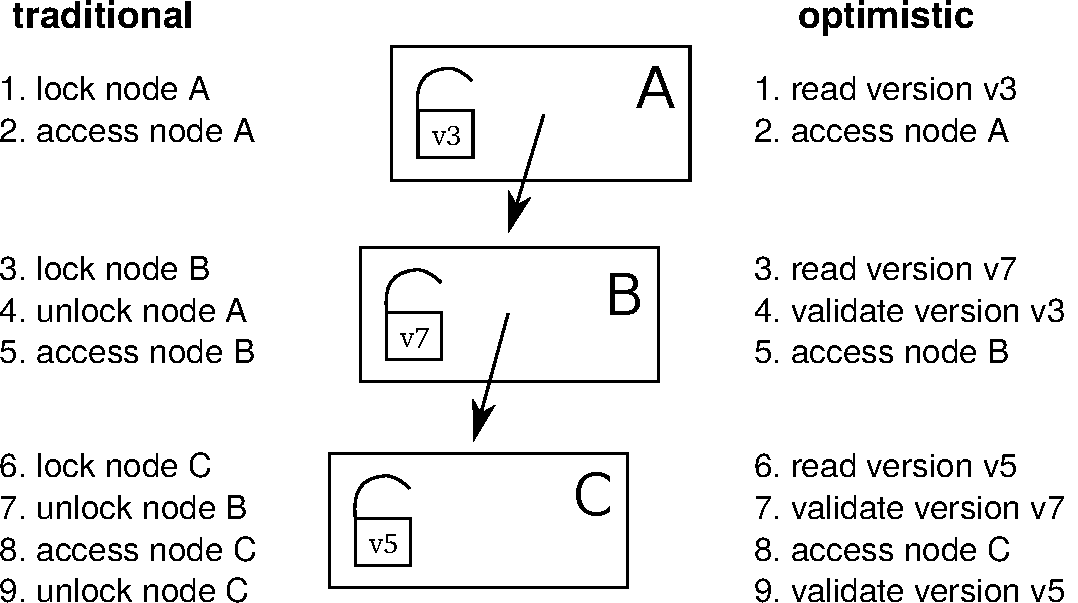
\includegraphics[width=0.65\linewidth]{olcall.pdf}
  \vspace{0.2cm}
  \caption{Comparison of a lookup operation in a 3-level tree using traditional lock coupling (left-hand side) vs.~optimistic lock coupling (right-hand side).}
  \label{fig:olc}
\end{figure}

The traditional and most common lock-based synchronization protocol for B-trees is lock coupling, which interleaves lock acquisitions while holding at most two locks at a time.
If, as we observed earlier, optimistic locks have similar semantics as traditional locks, it is natural to ask whether lock coupling can be combined with optimistic locks.
And indeed the answer is yes: One can almost mechanically translate traditional lock coupling code to optimistic lock coupling code.
This is illustrated in Figure~\ref{fig:olc}, which compares the traversal in a tree of height 3 using traditional and optimistic locks.
As the figure shows, the main difference is that locking is translated to reading the version and that unlocking becomes validation of the previously read version.
This simple change provides efficient lock-free tree traversal without the need to design a complex synchronization protocol.

It is important to emphasize the conceptual simplicity of OLC in comparison to data structures that use custom protocols like the Bw-tree~\cite{DBLP:conf/icde/LevandoskiLS13a}.
To implement lock-free access, the Bw-tree requires an indirection table, delta nodes, complex splitting and merging logic, retry logic, etc.
OLC, on the other hand, can directly be applied to B-trees mostly by adding the appropriate optimistic locking code and without modifying the node layout itself.
Therefore, OpenBw-Tree, an open source implementation of the Bw-tree, requires an order of magnitude more code than a B-tree based on OLC\footnote{Both implementations are available on GitHub: \url{https://github.com/wangziqi2016/index-microbench}}.
Given how difficult it is to develop, validate, and debug lock-free code, simplicity is obviously a major advantage.

\subsection{Correctness Aspects}

\begin{figure}
  % \centering
  %[basicstyle=\normalsize\ttfamily,showstringspaces=false,columns=fullflexible,breaklines=false,breakatwhitespace=true,numbers=none,numberstyle=\small,style=C,keepspaces=true]
\begin{lstlisting}[basicstyle=\ttfamily,language=C++,numbers=left,numberstyle=\small]
std::atomic<BTreeNode*> root;

// search for key in B+tree, returns payload in resultOut
bool lookup(Key key, Value& resultOut) {
   BTreeNode* node = root.load();
   uint64_t nodeVersion = node->readLockOrRestart();
   if (node != root.load()) // make sure the root is still the root
      restart();

   BTreeInner<Key>* parent = nullptr;
   uint64_t parentVersion = 0;

   while (node->isInner()) {
      auto inner = (BTreeInner*)node;

      // unlock parent and make current node the parent
      if (parent)
         parent->readUnlockOrRestart(parentVersion);
      parent = inner;
      parentVersion = nodeVersion;

      // search for next node
      node = inner->findChild(key);
      // validate 'inner' to ensure that 'node' pointer is valid
      inner->checkOrRestart(nodeVersion);
      // now it safe to dereference 'node' pointer (read its version)
      nodeVersion = node->readLockOrRestart();
   }

   // search in leaf and retrieve payload
   auto leaf = (BTreeLeaf*)node;
   bool success = leaf->findValue(key, resultOut);

   // unlock everything
   if (parent)
      parent->readUnlockOrRestart(parentVersion);
   node->readUnlockOrRestart(nodeVersion);

   return success;
}
\end{lstlisting}
  \vspace{0.2cm}
  \caption{B-tree lookup code using OLC. For simplicity, the restart logic is not shown.}
  \label{fig:lookup}
\end{figure}

So far, we have introduced the high-level ideas behind OLC and have stressed its similarity to traditional lock coupling.
Let us now discuss some cases where the close similarity between lock coupling and OLC breaks down.
To make this more concrete, we show the B-tree lookup code in Figure~\ref{fig:lookup}.
In the code, \texttt{readLockOrRestart} reads the lock version and \texttt{readUnlockOrRestart} validates that the read was correct.

One issue with OLC is that any pointer speculatively read from a node may point to invalid memory (if that node is modified concurrently).
Dereferencing such a pointer (e.g., to read its optimistic lock), may cause a segmentation fault or undefined behavior.
In the code shown in Figure~\ref{fig:lookup}, this problem is prevented by the extra check in line 25, which ensures that the read from the node containing the pointer was correct.
Without this additional validation, the code would in line 27 dereference the pointer speculatively read in line 23.
Note that the implementation of \texttt{checkOrRestart} is actually identical to \texttt{readUnlockOrRestart}.
We chose to give it a different name to highlight the fact that this extra check would not be necessary with read/write locks.

Another potential issue with optimistic locks is code that does not terminate.
Code that speculatively accesses a node, like an intra-node binary search, should be written in a way such that it always terminates---even in the presence of concurrent writes.
Otherwise, the validation code that detects the concurrent write will never run.
The binary search of a B-tree, for example, needs to be written in such a way that each comparison makes progress.
For some data structures that do not require loops in the traversal code (like ART) termination is trivially true.

\subsection{Implementation Details}

% implementation, efficiency
To implement an optimistic lock, one can combine the lock and the version counter into a single 64-bit\footnote{Even after subtracting one bit for the lock status, a back-of-the-envelope calculation can show that 63 bits are large enough to never overflow in practice.} word~\cite{artsync}.
A typical read operation will therefore merely consist of reading this version counter atomically.
In C++11 this can be implemented using the \texttt{std::atomic} type.

On x86, atomic reads are cheap because of x86's strong memory order guarantees.
No memory fences are required for sequentially-consistent loads, which are translated (by both GCC and clang) into standard \texttt{MOV} instructions.
Hence, the only effect of \texttt{std::atomic} for loads is preventing instruction re-ordering.
This makes version access and validation cheap.
Acquiring and releasing an optimistic lock in exclusive mode has comparable cost to a traditional lock:
A fairly expensive sequentially-consistent store is needed for acquiring a lock, while a standard \texttt{MOV} suffices for releasing it.
A simple sinlock-based implementation of optimistic locks can be found in the appendix of an earlier paper~\cite{artsync}.

OLC code must be able to handle restarts since validation or lock upgrade can fail due to concurrent writers.
Restarts can easily be implemented by wrapping the data structure operation in a loop (for simplicity not shown in Figure~\ref{fig:lookup}).
Such a loop also enables limiting the number of optimistic retry operations and falling back to pessimistic locking in cases of very heavy contention.
The ability to fall back to traditional locking is a major advantage of OLC in terms of robustness over lock-free approaches, which do not have this option.

In addition to the optimistic shared mode and the exclusive mode, optimistic locks also support a ``shared pessimistic'' mode, which physically acquires the lock in shared mode (allowing multiple concurrent readers but no writers).
This mode is useful for table (or range) scans that touch many tuples on a leaf page (which would otherwise easily abort).
Finally, let us mention that large range scans and table scans, should be broken up into several per-node traversals as is done in the LeanStore~\cite{leanstore} system.

Like all lock-free data structures, but unlike traditional locking and Hardware Transactional Memory~\cite{DBLP:conf/hpca/KarnagelDRLLSL14,DBLP:journals/pvldb/MakreshanskiLS15,htmtkde}, OLC requires care when deleting (and reusing) nodes.
The reason is that a deleting thread can never be sure that a node can be reclaimed because other threads might still be optimistically reading from that node.
Therefore, standard solutions like epoch-based reclamation~\cite{DBLP:conf/sosp/TuZKLM13}, hazard pointers~\cite{DBLP:journals/tpds/Michael04}, or optimized hazard pointers~\cite{DBLP:conf/spaa/BalmauGHZ16} need to be used.
These memory reclamation techniques are, however, largely orthogonal to the synchronization protocol itself.

%-lock-free is not a strong guarantee

\newpage
\section{Evaluation}\label{sec:evaluation}

Let us now experimentally evaluate the overhead and scalability of OLC.
For the experiments, we use an in-memory B+tree implemented in C++11 using templates, which is configured to use nodes of 4096 bytes, random 8 byte keys, and 8 byte payloads.
Based on this B-tree, we compare the following synchronization approaches:
\begin{itemize}
\item an OLC implementation\footnote{An almost identical OLC implementation is available on github: \url{https://github.com/wangziqi2016/index-microbench/tree/master/BTreeOLC}}
\item a variant based on traditional lock coupling and read/write locks
\item the unsynchronized B-tree, which obviously is only correct for read-only workloads but allows measuring the overhead of synchronization
\end{itemize}
Note that earlier work has compared the OLC implementation with a Bw-tree implementation~\cite{buzzword} and other state-of-the-art in-memory index structures.

We use a Haswell EP system with an Intel Xeon E5-2687W v3 CPU, which has 10 cores (20 ``Hyper-Threads'') and 25~MB of L3 cache.
The system is running Ubuntu 18.10 and we use GCC 8.2.0 to compile our code.
The CPU counters are obtained using the Linux perf API\footnote{We use the following convenience wrapper: \url{https://github.com/viktorleis/perfevent}}.

\begin{table}
  \caption{Performance and CPU counters for lookup and insert operations in a B-tree with 100M keys. We perform 100M operations and normalize the CPU counters by that number.}
  \label{tab:overhead}
  \centering
  \begin{tabular}{lrrrrrrr}\toprule
                    &         &        &        & instruc-  & L1     & L3     & branch \\
                    & threads & M op/s & cycles & tions & misses & misses & misses \\\midrule
lookup (no sync.)   & 1       & 1.72   & 2028   & 283     & 39.1   & 14.9   & 16.1   \\
lookup (OLC)        & 1       & 1.65   & 2107   & 370     & 43.9   & 15.1   & 16.7   \\
lookup (lock coup.) & 1       & 1.72   & 2078   & 365     & 42.3   & 16.9   & 15.7   \\\midrule
insert (no sync.)   & 1       & 1.51   & 2286   & 530     & 59.8   & 31.1   & 17.3   \\
insert (OLC)        & 1       & 1.50   & 2303   & 629     & 61.2   & 31.1   & 16.5   \\
insert (lock coup.) & 1       & 1.41   & 2473   & 644     & 61.0   & 31.0   & 17.2   \\\midrule
lookup (no sync.)   & 10      & 15.48  & 2058   & 283     & 38.6   & 15.5   & 16.0   \\
lookup (OLC)        & 10      & 14.60  & 2187   & 370     & 43.8   & 15.8   & 16.8   \\
lookup (lock coup.) & 10      & 5.71   & 5591   & 379     & 54.2   & 17.0   & 14.8   \\\midrule
insert (no sync.)   & 10      & -      & -      & -       & -      & -      & -      \\
insert (OLC)        & 10      & 10.46  & 2940   & 656     & 62.0   & 32.5   & 16.8   \\
insert (lock coup.) & 10      & 7.55   & 4161   & 667     & 75.0   & 28.6   & 16.2   \\
    \bottomrule
\end{tabular}
\end{table}

Table~\ref{tab:overhead} compares the performance and CPU counters for lookup and insert operations in a B-tree with 100M keys.
With {\em single-threaded} execution, we observe that all three approaches have very similar performance.
Adding traditional or optimistic locks to unsynchronized B-tree code results in up to 30\% of additional instructions without affecting single-threaded performance much.

\begin{figure}
  \centering
  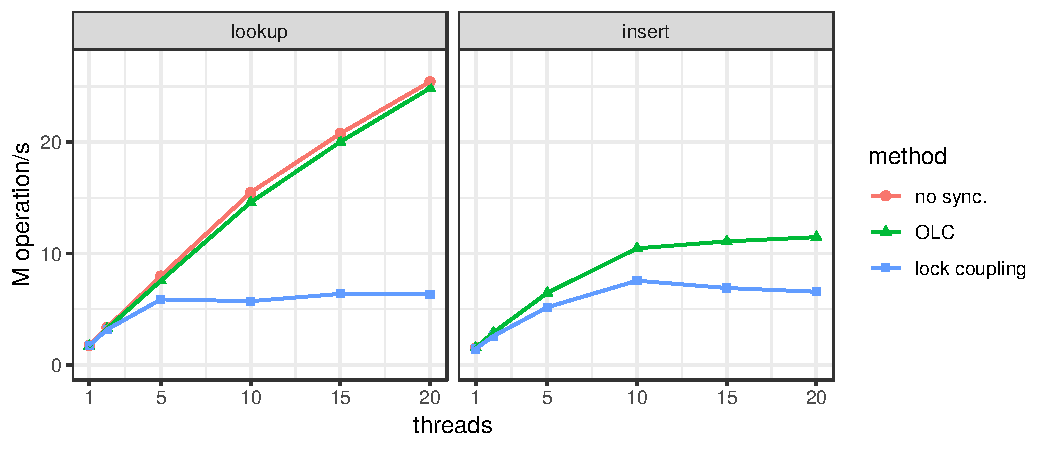
\includegraphics[width=\linewidth]{scale.pdf}
  \vspace{0.2cm}
  \caption{Scalability on 10-core system for B-tree operations (100M values).}
  \label{fig:scale}
\end{figure}

As Figure~\ref{fig:scale} shows, the results change dramatically once we use multiple threads.
For lookup, the scalability of OLC is near-linear up to 20 threads, even though the system has only 10 ``real cores''.
The OLC scalability for insert is also respectable (though not quite as linear because multi-threaded insertion approaches the memory bandwidth of our processor).
The figure also shows that the results of traditional lock coupling with read/write locks are significantly worse than OLC.
With 20 threads, lookup with OLC is 3.9$\times$ faster than traditional lock coupling.

\section{Summary}\label{sec:conc}

Optimistic Lock Coupling (OLC) is an effective synchronization method that combines the simplicity of traditional lock coupling with the superior scalability of lock-free approaches.
OLC is widely applicable and has already been successfully used to synchronize several data structures, including B-trees, binary search trees, and different trie variants.
These features make it highly attractive for modern database systems as well as performance-critical systems software in general.

\begin{thebibliography}{10}

\bibitem{DBLP:conf/spaa/BalmauGHZ16}
O.~Balmau, R.~Guerraoui, M.~Herlihy, and I.~Zablotchi.
\newblock Fast and robust memory reclamation for concurrent data structures.
\newblock In {\em SPAA}, 2016.

\bibitem{DBLP:journals/acta/BayerS77}
R.~Bayer and M.~Schkolnick.
\newblock Concurrency of operations on {B}-trees.
\newblock {\em Acta Informatica}, 9, 1977.

\bibitem{hot}
R.~Binna, E.~Zangerle, M.~Pichl, G.~Specht, and V.~Leis.
\newblock {HOT}: A height optimized trie index for main-memory database
  systems.
\newblock In {\em SIGMOD}, 2018.

\bibitem{DBLP:conf/ppopp/BronsonCCO10}
N.~G. Bronson, J.~Casper, H.~Chafi, and K.~Olukotun.
\newblock A practical concurrent binary search tree.
\newblock In {\em PPOPP}, 2010.

\bibitem{DBLP:conf/vldb/ChaHKK01}
S.~K. Cha, S.~Hwang, K.~Kim, and K.~Kwon.
\newblock Cache-conscious concurrency control of main-memory indexes on
  shared-memory multiprocessor systems.
\newblock In {\em VLDB}, 2001.

\bibitem{intel}
I.~Cutress.
\newblock {Intel} goes for 48-cores: {Cascade-AP} with multi-chip package
  coming soon.
\newblock
  \url{https://www.anandtech.com/show/13535/intel-goes-for-48cores-cascade-ap},
  2018 (accessed January, 2019).

\bibitem{DBLP:conf/cidr/FaleiroA17}
J.~M. Faleiro and D.~J. Abadi.
\newblock Latch-free synchronization in database systems: Silver bullet or
  fool's gold?
\newblock In {\em CIDR}, 2017.

\bibitem{DBLP:journals/ftdb/Graefe11}
G.~Graefe.
\newblock Modern {B}-tree techniques.
\newblock {\em Foundations and Trends in Databases}, 3(4), 2011.

\bibitem{DBLP:conf/hpca/KarnagelDRLLSL14}
T.~Karnagel, R.~Dementiev, R.~Rajwar, K.~Lai, T.~Legler, B.~Schlegel, and
  W.~Lehner.
\newblock Improving in-memory database index performance with
  {Intel}\({}^{\mbox{{\textregistered}}}\) transactional synchronization
  extensions.
\newblock In {\em HPCA}, 2014.

\bibitem{DBLP:journals/tods/LehmanY81}
P.~L. Lehman and S.~B. Yao.
\newblock Efficient locking for concurrent operations on {B}-trees.
\newblock {\em {ACM} Trans. Database Syst.}, 6(4), 1981.

\bibitem{leanstore}
V.~Leis, M.~Haubenschild, A.~Kemper, and T.~Neumann.
\newblock Leanstore: In-memory data management beyond main memory.
\newblock In {\em ICDE}, 2018.

\bibitem{art}
V.~Leis, A.~Kemper, and T.~Neumann.
\newblock The adaptive radix tree: {ARTful} indexing for main-memory databases.
\newblock In {\em ICDE}, 2013.

\bibitem{htmtkde}
V.~Leis, A.~Kemper, and T.~Neumann.
\newblock Scaling {HTM}-supported database transactions to many cores.
\newblock {\em {IEEE} Trans. Knowl. Data Eng.}, 28(2), 2016.

\bibitem{artsync}
V.~Leis, F.~Scheibner, A.~Kemper, and T.~Neumann.
\newblock The {ART} of practical synchronization.
\newblock In {\em DaMoN}, 2016.

\bibitem{DBLP:conf/icde/LevandoskiLS13a}
J.~J. Levandoski, D.~B. Lomet, and S.~Sengupta.
\newblock The {Bw}-tree: A {B}-tree for new hardware platforms.
\newblock In {\em ICDE}, 2013.

\bibitem{DBLP:journals/pvldb/MakreshanskiLS15}
D.~Makreshanski, J.~J. Levandoski, and R.~Stutsman.
\newblock To lock, swap, or elide: On the interplay of hardware transactional
  memory and lock-free indexing.
\newblock {\em {PVLDB}}, 8(11), 2015.

\bibitem{DBLP:dblp_conf/eurosys/MaoKM12}
Y.~Mao, E.~Kohler, and R.~T. Morris.
\newblock Cache craftiness for fast multicore key-value storage.
\newblock In {\em EuroSys}, 2012.

\bibitem{DBLP:journals/tpds/Michael04}
M.~M. Michael.
\newblock Hazard pointers: Safe memory reclamation for lock-free objects.
\newblock {\em {IEEE} Trans. Parallel Distrib. Syst.}, 15(6), 2004.

\bibitem{DBLP:journals/jacm/ShalevS06}
O.~Shalev and N.~Shavit.
\newblock Split-ordered lists: Lock-free extensible hash tables.
\newblock {\em J. {ACM}}, 53(3), 2006.

\bibitem{amd}
A.~Shilov.
\newblock {AMD} previews {EPYC} ‘{Rome}’ processor: Up to 64 {Zen} 2 cores.
\newblock
  \url{https://www.anandtech.com/show/13561/amd-previews-epyc-rome-processor-up-to-64-zen-2-cores},
  2018 (accessed January, 2019).

\bibitem{DBLP:conf/sosp/TuZKLM13}
S.~Tu, W.~Zheng, E.~Kohler, B.~Liskov, and S.~Madden.
\newblock Speedy transactions in multicore in-memory databases.
\newblock In {\em SOSP}, 2013.

\bibitem{buzzword}
Z.~Wang, A.~Pavlo, H.~Lim, V.~Leis, H.~Zhang, M.~Kaminsky, and D.~Andersen.
\newblock Building a {Bw}-tree takes more than just buzz words.
\newblock In {\em SIGMOD}, 2018.

\end{thebibliography}


%\bibliographystyle{abbrv}
%\bibliography{main}

\end{document}

\end{article}

\begin{article}
{Evaluating the Factuality of Large Language Models using Large-Scale Knowledge Graphs}
{Xiaoze Liu, Feijie Wu, Tianyang Xu, Zhuo Chen, Yichi Zhang, Xiaoqian Wang, Jing Gao}
\setcounter{section}{0}
\NeedsTeXFormat{LaTeX2e} 
\ProvidesPackage{debulletin}[2002/04/01 Data Engineering Bulletin package]
% \RequirePackage{epsfig}

%%%%%%%%%%%%%%%%%%%%%%%%%%%%%%%%%%%%%%%%%%%%%%%%%%%%%%%%%%%%%%%%%%%%%%%%
%%
%% INTRODUCTION
%%
%%%%%%%%%%%%%%%%%%%%%%%%%%%%%%%%%%%%%%%%%%%%%%%%%%%%%%%%%%%%%%%%%%%%%%%%
% 
% This is a LaTeX package for the Bulletin of the Technical Committee on
% Data Engineering.  It is intended to be used with the article document
% class at 11pt, but it can probably be used with report and book classes
% and other font sizes as well.
% The expected format of the bulletin is
% 
% 1. A cover.  This includes:
%    - a front cover page with the title, date, volume, and number of 
%      the issue, and with the table of contents
%    - an inside cover page giving the names of the editors and committee 
%      members, and other information
%    - an inside back cover that is blank
%    - a back cover that is blank, except for the IEEE mailing address and
%      the postage permit just below the fold half way down the page.
% 2. A few miscellaneous columns, probably from the editor of the special
%    issue and an overview of the area covered by the special issue.
% 3. A few letters to the editor.
% 4. The contributed articles
% 5. A few calls for papers for coming conference.
% 
% An example of how such an issue is as follows.
% Note that there are several formatting paramters, and they are described
% at the end of this file.
%
%%%%%%%%%%%%%%%%%%%%%%%%%%%%%%%%%%%%%%%%%%%%%%%%%%%%%%%%%%%%%%%%%%%%%%%%
%
% \documentclass[11pt]{article}
% \usepackage{debulletin}
% \begin{document}
% 
% \bulletindate{March 2002}
% \bulletinvolume{1}
% \bulletinnumber{1}
% \bulletinyear{2002}
% \begin{bulletin}
% 
% %
% %  Introductory columns.  In table of contents, we want a heading 
% %  ``Introduction'' followed by subheadings (that is, table of contents 
% %  subentries) for each of the two columns.  Inside the bulletin, we
% %  want each column preceded by a heading giving the title of the column.
% %
% \tocheading{Introduction}
% 
% \heading{A letter from the Editor}
% \tocsubentry{A letter from the Editor}{I. M. Editor}
% \input{editorletter}
% 
% \heading{Easy-to-use Databases: a Tutorial}
% \tocsubentry{Easy-to-use Databases: a Tutorial}{I. M. Expert}
% \input{tutorial}
% 
% %
% %  Letters to the editor section.  Use the lettersection environment.
% %  Each letter is contained in a letter environment, where the two required
% %  options to \begin{letter} are the author and the address of the author.
% %
% \begin{lettersection}
% 
% \begin{letter}{My database is better than yours}{D. B. Hacker}%
% 					{Hacker, Inc. \\ Cambridge, MA}
% \input{dbhacker}
% \end{letter}
% 
% \begin{letter}{No it isn't}{Betty D. Hacker}{Betty, Inc. \\ Palo Alto, CA}
% \input{bdhacker}
% \end{letter}
% 
% \end{lettersection}
% 
% %
% %  Contributed articles section.  Use the articlesection environment.
% %  The argument to the articlesection command is TOPIC, where the name
% %  of the special issue is supposed to be ``Special Issue on TOPIC''.
% %  Each article is contained in an article environment, where the two 
% %  required options to \begin{article} are the title and author of 
% %  the article.
% %
% \begin{articlesection}{Easy-to-Use Databases}
% 
% \begin{article}{Easy Data Entry}{David Crowbar}
% \input{crowbar}
% \end{article}
% 
% \begin{article}{Data Security made Simple}{General Confusion}
% \input{confusion}
% \end{article}
% 
% \end{articlesection}
% 
% %
% %  Calls for papers section.  Use the callsection environment.
% %  Each call for papers is contained in an call environment, where the single 
% %  required options to \begin{call} is the name of the conference.
% %
% \begin{callsection}
% \begin{call}{DB Conference A}
% \input{dba}
% \end{call}
% 
% \begin{call}{DB Conference B}
% \input{dbb}
% \end{call}
% \end{callsection}
% 
% \end{bulletin}
% \end{document}
%
%%%%%%%%%%%%%%%%%%%%%%%%%%%%%%%%%%%%%%%%%%%%%%%%%%%%%%%%%%%%%%%%%%%%%%%%

%%%%%%%%%%%%%%%%%%%%%%%%%%%%%%%%%%%%%%%%%%%%%%%%%%%%%%%%%%%%%%%%%%%%%%%%
% 
% The bulletin environment.
% 
% The bulletin environment generates the covers.  The two sides of the
% front cover are generated by \begin{bulletin}, and the two sides of
% the back cover are generated by \end{bulletin}.
%
%%%%%%%%%%%%%%%%%%%%%%%%%%%%%%%%%%%%%%%%%%%%%%%%%%%%%%%%%%%%%%%%%%%%%%%%

\newenvironment{bulletin}%
  {\@MakeCoverOne\@MakeCoverTwo}%
  {\cleardoublepage
   \@MakeCoverThree\@MakeCoverFour
  }
%
% The outside front cover
%
\newcommand{\@MakeCoverOne}{
  \begingroup
    \@SetCoverDimensions
    \begin{titlepage}
      \thispagestyle{empty}
      %\vbox{}\vskip .5in
      \textbf{\Large Bulletin of the Technical Committee on}
      \par\bigskip
      \textbf{\@namefontsize Data}
      \par\medskip
      \textbf{\@namefontsize Engineering}
      \par\bigskip
      \textbf{\Large \@BulletinDate \quad Vol. \@BulletinVolume{} No. 
        \@BulletinNumber \hfill \@includeIEEElogo IEEE Computer Society}
      \par\bigskip
      \hrule
      \par
%      \bigskip
      \tableofcontents
      \vfil
    \end{titlepage}
  \endgroup
}
\newcommand{\@BulletinDate}{June 2018}
\newcommand{\@BulletinNumber}{2}
\newcommand{\@BulletinVolume}{41}
\newcommand{\@BulletinYear}{2018}
\newcommand{\bulletindate}[1]{\renewcommand{\@BulletinDate}{#1}} 
\newcommand{\bulletinnumber}[1]{\renewcommand{\@BulletinNumber}{#1}}
\newcommand{\bulletinvolume}[1]{\renewcommand{\@BulletinVolume}{#1}}
\newcommand{\bulletinyear}[1]{\renewcommand{\@BulletinYear}{#1}}

%
% The inside front cover
% 
\newcommand{\@MakeCoverTwo}{
  \begingroup
    \@SetCoverDimensions
    \@includeinsidefront 
  \endgroup
}
%
% The inside back cover
% 
\newcommand{\@MakeCoverThree}{
  \begingroup
    \@SetCoverDimensions
    \@includeinsideback 
  \endgroup
}
%
% The outside back cover
% 
\newcommand{\@MakeCoverFour}{
  \begingroup
    \@SetCoverDimensions
    \begin{titlepage}
      \thispagestyle{empty}
      \vbox{}\vskip .5\coverheight
      \hbox to \hsize{\@PrintIEEEAddress \hfill \@PrintPostagePermit}
      \vfil
    \end{titlepage}
  \endgroup
}
\newcommand{\@PrintIEEEAddress}{\hbox to 0pt{\vbox{\@IEEEAddress}\hss}}
\newcommand{\@PrintPostagePermit}{\hbox to 0pt{\hss\framebox{\hbox to 1.25in
  {\hss\vbox to 1.25in{\hsize 1.25in \center \vss \@PostagePermit \vss}}}}}
\newcommand{\@IEEEAddress}{}	  
\newcommand{\@PostagePermit}{}
\newcommand{\IEEEAddress}[1]{\renewcommand{\@IEEEAddress}{#1}} 
\newcommand{\PostagePermit}[1]{\renewcommand{\@PostagePermit}{#1}}  
%
% Compute cover layout dimentions
%
% Reset \oddsidemargin, \evensidemargin, and \topmargin so that the covers
% are centered on the physical page.
% The height and width of the physical page are determined by 
% \physicalpageheight and \physicalpagewidth.
% The height and width of text on the cover are determined by \coverheight
% and \coverwidth.
%
\newcommand{\@SetCoverDimensions}{%
  \hsize \coverwidth
  \oddsidemargin \physicalpagewidth
  \advance \oddsidemargin by -\coverwidth
  \divide \oddsidemargin by 2%
  \advance \oddsidemargin by -1in%
  \evensidemargin \oddsidemargin
  %
  \vsize \coverheight
  \topmargin \physicalpageheight
  \advance \topmargin by -\coverheight
  \divide \topmargin by 2%
  \advance \topmargin by -\topskip
  \advance \topmargin by -\headheight
  \advance \topmargin by -\headsep
  \advance \topmargin by -1in%
  %
  \parindent 0pt%
  \parskip   0pt%
}

%%%%%%%%%%%%%%%%%%%%%%%%%%%%%%%%%%%%%%%%%%%%%%%%%%%%%%%%%%%%%%%%%%%%%%%%%%
%
%  The LETTER SECTION.
%
% The section is enclosed between \begin{lettersection} and \end{lettersection}
% commands, and each letter is enclosed between 
% \begin{letter}{TITLE}{AUTHOR}{ADDRESS} and \end{letter} commands where
% TITLE and AUTHOR are the title and author of the letter and ADDRESS is
% the ADDRESS of the author (complete with \\ separating lines of the address
% as usual).
%
%%%%%%%%%%%%%%%%%%%%%%%%%%%%%%%%%%%%%%%%%%%%%%%%%%%%%%%%%%%%%%%%%%%%%%%%%%

\newenvironment{lettersection}%
       {\clearpage
%	\tocskip{\bigskipamount}
	\tocheading{\strut Letters}
	\tocskip{\smallskipamount}
	\pageheading{Letters}{Letters}
	\thispagestyle{plain}
	}%
       {\clearpage}
\newenvironment{letter}[3]
       {\newcommand{\lettertitle}{#1}
	\newcommand{\letterauthor}{#2}
	\newcommand{\letteraddress}{#3}
	\tocsubentry{\lettertitle}{\letterauthor}
	\heading{\lettertitle}
	\makeatletter
        \@RestoreMaketitle
	\@UndefinePreambleCommands
	\NeedsTeXFormat{LaTeX2e}
\ProvidesPackage{deauthor}[2002/04/01 Data Engineering Bulletin Author package]

%
% Undefine the \date command, so no date is printed with the title
%
\renewcommand{\date}[1]{}
\renewcommand{\@date}{\@empty}

%
% Undefine the titlepage environment so that articles don't try to
% circumvent the journal's formatting conventions for the first page.
% This works for the article class, but causes trouble for reports and 
% books since the \maketitle command is defined in terms of the titlepage 
% environment.
%
\renewenvironment{titlepage}{}{}

%
% Undefine the \pagestyle and \thispagestyle commands so that articles
% don't try to change the page style.
%
\renewcommand{\pagestyle}[1]{}
\renewcommand{\thispagestyle}[1]{}

%
% Define common theorem-like environment created with the \newtheorem
% command.  First we have to undefine them all since we just defined them
% in the previous article.  Also, define a proof environment and a \qed
% symbol to end the proof.
%
% This initial hack redefines the theorem-like environments of latex to
% follow the theorem heading with a colon (e.g. Theorem 4:) and print
% the theorem text in roman font.
%
\renewcommand{\@begintheorem}[2]%
        {\trivlist \item[\hskip \labelsep{\bf #1\ #2:}]}
\renewcommand{\@opargbegintheorem}[3]%
        {\trivlist \item[\hskip \labelsep{\bf #1\ #2\ (#3):}]}
%
\let\theorem\relax
\let\lemma\relax
\let\corollary\relax
\let\proposition\relax
\let\claim\relax
\let\definition\relax
\let\proof\relax \let\endproof\relax
%
\newtheorem{theorem}{Theorem}
\newtheorem{lemma}[theorem]{Lemma}
\newtheorem{corollary}[theorem]{Corollary}
\newtheorem{proposition}[theorem]{Proposition}
\newtheorem{claim}[theorem]{Claim}
\newtheorem{definition}[theorem]{Definition}
%
\newenvironment{proof}{\noindent {\bf Proof:}}{}
\newcommand{\squarebox}[1]{\hbox to #1{\hfill\vbox to #1{\vfill}}}
\newcommand{\qed}{\hspace*{\fill}
            \vbox{\hrule\hbox{\vrule\squarebox{.667em}\vrule}\hrule}\smallskip}

%
% Define an example environment, just another theorem environment but with
% independent numbering.
%
\let\example\relax
\newtheorem{example}{Example}

%
% Define an indented abstract environment.
%
\renewenvironment{abstract}%
  {\begin{center}\textbf{Abstract}\end{center}\narrower\itshape}%
  {\par}  

% 
% Reset all section and figure counters so that an article's section
% and figure numbers begin with 1.
%
\setcounter{section}{0}
\setcounter{figure}{0}
\setcounter{table}{0}


%
% Place page formatting parameters (like page dimensions) here
% These should match the dimensions in bulletin.sty.
%
\textheight     9.0in
\textwidth      6.75in
\oddsidemargin  0.0in
\evensidemargin -0.25in
\topmargin      0.0in
\headheight     0.0in
\headsep        0.0in
%\footheight     0.0in

\@twosidetrue        % print on two sides of a page

%
% Authors are not supposed to change page dimensions.
%

\let\@setlength\setlength       % save old definition
\renewcommand{\setlength}[2]{%
  \@VerifyChangeableLength{#1}%
  \if@ChangeableLength\@setlength{#1}{#2}\else\@UnchangeableError{#1}\fi}

\let\@addtolength\addtolength   % save old definition
\renewcommand{\addtolength}[2]{%
  \@VerifyChangeableLength{#1}%
  \if@ChangeableLength\@addtolength{#1}{#2}\else\@UnchangeableError{#1}\fi}

\let\@settowidth\settowidth     % save old definition
\renewcommand{\settowidth}[2]{%
  \@VerifyChangeableLength{#1}%
  \if@ChangeableLength\@settowidth{#1}{#2}\else\@UnchangeableError{#1}\fi}

\newif\if@ChangeableLength      \@ChangeableLengthtrue
\newcommand{\@VerifyChangeableLength}[1]{%
  \ifx#1\textwidth              \@ChangeableLengthfalse
  \else\ifx#1\textheight        \@ChangeableLengthfalse
  \else\ifx#1\textwidth         \@ChangeableLengthfalse
  \else\ifx#1\oddsidemargin     \@ChangeableLengthfalse
  \else\ifx#1\evensidemargin    \@ChangeableLengthfalse
  \else\ifx#1\topmargin         \@ChangeableLengthfalse
  \else\ifx#1\headheight        \@ChangeableLengthfalse
  \else\ifx#1\headsep           \@ChangeableLengthfalse
  \else\ifx#1\footheight        \@ChangeableLengthfalse
  \else\@ChangeableLengthtrue\fi\fi\fi\fi\fi\fi\fi\fi\fi}
\newcommand{\@UnchangeableError}[1]{%
  \errmessage{Error: Authors are not allowed to change #1.. Ignored}}

%
% We want the title to be typeset in boldface, and the author names
% to be typeset in italics.  We can hardwire this for the title,
% but trying to do the same thing for the author causes confusion
% due to the use of \@author in \@maketitle in article.sty.
% 
% We also want to print a copyright notice and the bulletin title at
% the bottom of every first page.
%
\renewcommand{\title}[1]{%
  \gdef\@title{\textbf{#1}}
  \begingroup 
  \renewcommand{\thefootnote}{\fnsymbol{footnote}}
  \global\setcounter{footnote}{0}
  \footnotetext{%
    \emph{Copyright {\@BulletinYear} IEEE. Personal use of this material is
    permitted. However, permission to reprint/republish this material for
    advertising or promotional purposes or for creating new collective
    works for resale or redistribution to servers or lists, or to reuse
    any copyrighted component of this work in other works must be obtained
    from the IEEE.}\\
    \textbf{Bulletin of the IEEE Computer Society Technical Committee on
    Data Engineering} \\
    \footnoterule
  }%
  \endgroup
}
\providecommand{\@BulletinYear}{0000}
\providecommand{\bulletinyear}[1]{\renewcommand{\@BulletinYear}{#1}}

  % read in the author style file
	\makeatother
	}%
       {\par\nobreak\vspace{\medskipamount}\noindent
             \vbox{\raggedleft\letterauthor\\\letteraddress\par}\vskip 1in}

\newenvironment{awardsection}
       {\clearpage
	\tocskip{\bigskipamount}
	\tocrule
%	\tocskip{\bigskipamount}
	\tocheading{\strut 2019 IEEE TCDE Awards}
	\tocskip{\smallskipamount}
	\pageheading{2019 IEEE TCDE Awards}{2019 IEEE TCDE Awards}
	\thispagestyle{plain}
	}%
       {\clearpage}
\newenvironment{award}[3]
       {\newcommand{\awardtitle}{#1}
	\newcommand{\awardauthor}{#2}
	\newcommand{\awardaddress}{#3}
	\tocsubentry{\awardtitle}{\awardauthor}
	\heading{\awardtitle}
	\makeatletter
        \@RestoreMaketitle
	\@UndefinePreambleCommands
	\NeedsTeXFormat{LaTeX2e}
\ProvidesPackage{deauthor}[2002/04/01 Data Engineering Bulletin Author package]

%
% Undefine the \date command, so no date is printed with the title
%
\renewcommand{\date}[1]{}
\renewcommand{\@date}{\@empty}

%
% Undefine the titlepage environment so that articles don't try to
% circumvent the journal's formatting conventions for the first page.
% This works for the article class, but causes trouble for reports and 
% books since the \maketitle command is defined in terms of the titlepage 
% environment.
%
\renewenvironment{titlepage}{}{}

%
% Undefine the \pagestyle and \thispagestyle commands so that articles
% don't try to change the page style.
%
\renewcommand{\pagestyle}[1]{}
\renewcommand{\thispagestyle}[1]{}

%
% Define common theorem-like environment created with the \newtheorem
% command.  First we have to undefine them all since we just defined them
% in the previous article.  Also, define a proof environment and a \qed
% symbol to end the proof.
%
% This initial hack redefines the theorem-like environments of latex to
% follow the theorem heading with a colon (e.g. Theorem 4:) and print
% the theorem text in roman font.
%
\renewcommand{\@begintheorem}[2]%
        {\trivlist \item[\hskip \labelsep{\bf #1\ #2:}]}
\renewcommand{\@opargbegintheorem}[3]%
        {\trivlist \item[\hskip \labelsep{\bf #1\ #2\ (#3):}]}
%
\let\theorem\relax
\let\lemma\relax
\let\corollary\relax
\let\proposition\relax
\let\claim\relax
\let\definition\relax
\let\proof\relax \let\endproof\relax
%
\newtheorem{theorem}{Theorem}
\newtheorem{lemma}[theorem]{Lemma}
\newtheorem{corollary}[theorem]{Corollary}
\newtheorem{proposition}[theorem]{Proposition}
\newtheorem{claim}[theorem]{Claim}
\newtheorem{definition}[theorem]{Definition}
%
\newenvironment{proof}{\noindent {\bf Proof:}}{}
\newcommand{\squarebox}[1]{\hbox to #1{\hfill\vbox to #1{\vfill}}}
\newcommand{\qed}{\hspace*{\fill}
            \vbox{\hrule\hbox{\vrule\squarebox{.667em}\vrule}\hrule}\smallskip}

%
% Define an example environment, just another theorem environment but with
% independent numbering.
%
\let\example\relax
\newtheorem{example}{Example}

%
% Define an indented abstract environment.
%
\renewenvironment{abstract}%
  {\begin{center}\textbf{Abstract}\end{center}\narrower\itshape}%
  {\par}  

% 
% Reset all section and figure counters so that an article's section
% and figure numbers begin with 1.
%
\setcounter{section}{0}
\setcounter{figure}{0}
\setcounter{table}{0}


%
% Place page formatting parameters (like page dimensions) here
% These should match the dimensions in bulletin.sty.
%
\textheight     9.0in
\textwidth      6.75in
\oddsidemargin  0.0in
\evensidemargin -0.25in
\topmargin      0.0in
\headheight     0.0in
\headsep        0.0in
%\footheight     0.0in

\@twosidetrue        % print on two sides of a page

%
% Authors are not supposed to change page dimensions.
%

\let\@setlength\setlength       % save old definition
\renewcommand{\setlength}[2]{%
  \@VerifyChangeableLength{#1}%
  \if@ChangeableLength\@setlength{#1}{#2}\else\@UnchangeableError{#1}\fi}

\let\@addtolength\addtolength   % save old definition
\renewcommand{\addtolength}[2]{%
  \@VerifyChangeableLength{#1}%
  \if@ChangeableLength\@addtolength{#1}{#2}\else\@UnchangeableError{#1}\fi}

\let\@settowidth\settowidth     % save old definition
\renewcommand{\settowidth}[2]{%
  \@VerifyChangeableLength{#1}%
  \if@ChangeableLength\@settowidth{#1}{#2}\else\@UnchangeableError{#1}\fi}

\newif\if@ChangeableLength      \@ChangeableLengthtrue
\newcommand{\@VerifyChangeableLength}[1]{%
  \ifx#1\textwidth              \@ChangeableLengthfalse
  \else\ifx#1\textheight        \@ChangeableLengthfalse
  \else\ifx#1\textwidth         \@ChangeableLengthfalse
  \else\ifx#1\oddsidemargin     \@ChangeableLengthfalse
  \else\ifx#1\evensidemargin    \@ChangeableLengthfalse
  \else\ifx#1\topmargin         \@ChangeableLengthfalse
  \else\ifx#1\headheight        \@ChangeableLengthfalse
  \else\ifx#1\headsep           \@ChangeableLengthfalse
  \else\ifx#1\footheight        \@ChangeableLengthfalse
  \else\@ChangeableLengthtrue\fi\fi\fi\fi\fi\fi\fi\fi\fi}
\newcommand{\@UnchangeableError}[1]{%
  \errmessage{Error: Authors are not allowed to change #1.. Ignored}}

%
% We want the title to be typeset in boldface, and the author names
% to be typeset in italics.  We can hardwire this for the title,
% but trying to do the same thing for the author causes confusion
% due to the use of \@author in \@maketitle in article.sty.
% 
% We also want to print a copyright notice and the bulletin title at
% the bottom of every first page.
%
\renewcommand{\title}[1]{%
  \gdef\@title{\textbf{#1}}
  \begingroup 
  \renewcommand{\thefootnote}{\fnsymbol{footnote}}
  \global\setcounter{footnote}{0}
  \footnotetext{%
    \emph{Copyright {\@BulletinYear} IEEE. Personal use of this material is
    permitted. However, permission to reprint/republish this material for
    advertising or promotional purposes or for creating new collective
    works for resale or redistribution to servers or lists, or to reuse
    any copyrighted component of this work in other works must be obtained
    from the IEEE.}\\
    \textbf{Bulletin of the IEEE Computer Society Technical Committee on
    Data Engineering} \\
    \footnoterule
  }%
  \endgroup
}
\providecommand{\@BulletinYear}{0000}
\providecommand{\bulletinyear}[1]{\renewcommand{\@BulletinYear}{#1}}

  % read in the author style file
	\makeatother
	}%
       {\par\nobreak\vspace{\medskipamount}\noindent
             \vbox{\raggedleft\awardauthor\\\awardaddress\par}\vskip 1in}

%%%%%%%%%%%%%%%%%%%%%%%%%%%%%%%%%%%%%%%%%%%%%%%%%%%%%%%%%%%%%%%%%%%%%%%%%%

%%%%%%%%%%%%%%%%%%%%%%%%%%%%%%%%%%%%%%%%%%%%%%%%%%%%%%%%%%%%%%%%%%%%%%%%%%
%
%  The NEWS SECTION.
%
% The section is enclosed between \begin{newssection} and \end{newssection}
% commands, and each news item is enclosed between 
% \begin{news}{TITLE}{AUTHOR}{ADDRESS} and \end{news} commands where
% TITLE and AUTHOR are the title and author of the news and ADDRESS is
% the ADDRESS of the author (complete with \\ separating lines of the address
% as usual).
%
%%%%%%%%%%%%%%%%%%%%%%%%%%%%%%%%%%%%%%%%%%%%%%%%%%%%%%%%%%%%%%%%%%%%%%%%%%



\newenvironment{newssection}[1]%
       {\clearpage
%	\tocskip{\bigskipamount}
%	\tocrule
	\tocheading{\strut News: #1}
%\tocrule
	\tocskip{\smallskipamount}
	}%
       {\clearpage}

\newenvironment{news}[3]
       {\newcommand{\newstitle}{#1}
	\newcommand{\newsauthor}{#2}
	\newcommand{\newsaddress}{#3}
	\tocsubentry{\newstitle}{\newsauthor}
	\heading{\newstitle}
	\makeatletter
        \@RestoreMaketitle
	\@UndefinePreambleCommands
	\NeedsTeXFormat{LaTeX2e}
\ProvidesPackage{deauthor}[2002/04/01 Data Engineering Bulletin Author package]

%
% Undefine the \date command, so no date is printed with the title
%
\renewcommand{\date}[1]{}
\renewcommand{\@date}{\@empty}

%
% Undefine the titlepage environment so that articles don't try to
% circumvent the journal's formatting conventions for the first page.
% This works for the article class, but causes trouble for reports and 
% books since the \maketitle command is defined in terms of the titlepage 
% environment.
%
\renewenvironment{titlepage}{}{}

%
% Undefine the \pagestyle and \thispagestyle commands so that articles
% don't try to change the page style.
%
\renewcommand{\pagestyle}[1]{}
\renewcommand{\thispagestyle}[1]{}

%
% Define common theorem-like environment created with the \newtheorem
% command.  First we have to undefine them all since we just defined them
% in the previous article.  Also, define a proof environment and a \qed
% symbol to end the proof.
%
% This initial hack redefines the theorem-like environments of latex to
% follow the theorem heading with a colon (e.g. Theorem 4:) and print
% the theorem text in roman font.
%
\renewcommand{\@begintheorem}[2]%
        {\trivlist \item[\hskip \labelsep{\bf #1\ #2:}]}
\renewcommand{\@opargbegintheorem}[3]%
        {\trivlist \item[\hskip \labelsep{\bf #1\ #2\ (#3):}]}
%
\let\theorem\relax
\let\lemma\relax
\let\corollary\relax
\let\proposition\relax
\let\claim\relax
\let\definition\relax
\let\proof\relax \let\endproof\relax
%
\newtheorem{theorem}{Theorem}
\newtheorem{lemma}[theorem]{Lemma}
\newtheorem{corollary}[theorem]{Corollary}
\newtheorem{proposition}[theorem]{Proposition}
\newtheorem{claim}[theorem]{Claim}
\newtheorem{definition}[theorem]{Definition}
%
\newenvironment{proof}{\noindent {\bf Proof:}}{}
\newcommand{\squarebox}[1]{\hbox to #1{\hfill\vbox to #1{\vfill}}}
\newcommand{\qed}{\hspace*{\fill}
            \vbox{\hrule\hbox{\vrule\squarebox{.667em}\vrule}\hrule}\smallskip}

%
% Define an example environment, just another theorem environment but with
% independent numbering.
%
\let\example\relax
\newtheorem{example}{Example}

%
% Define an indented abstract environment.
%
\renewenvironment{abstract}%
  {\begin{center}\textbf{Abstract}\end{center}\narrower\itshape}%
  {\par}  

% 
% Reset all section and figure counters so that an article's section
% and figure numbers begin with 1.
%
\setcounter{section}{0}
\setcounter{figure}{0}
\setcounter{table}{0}


%
% Place page formatting parameters (like page dimensions) here
% These should match the dimensions in bulletin.sty.
%
\textheight     9.0in
\textwidth      6.75in
\oddsidemargin  0.0in
\evensidemargin -0.25in
\topmargin      0.0in
\headheight     0.0in
\headsep        0.0in
%\footheight     0.0in

\@twosidetrue        % print on two sides of a page

%
% Authors are not supposed to change page dimensions.
%

\let\@setlength\setlength       % save old definition
\renewcommand{\setlength}[2]{%
  \@VerifyChangeableLength{#1}%
  \if@ChangeableLength\@setlength{#1}{#2}\else\@UnchangeableError{#1}\fi}

\let\@addtolength\addtolength   % save old definition
\renewcommand{\addtolength}[2]{%
  \@VerifyChangeableLength{#1}%
  \if@ChangeableLength\@addtolength{#1}{#2}\else\@UnchangeableError{#1}\fi}

\let\@settowidth\settowidth     % save old definition
\renewcommand{\settowidth}[2]{%
  \@VerifyChangeableLength{#1}%
  \if@ChangeableLength\@settowidth{#1}{#2}\else\@UnchangeableError{#1}\fi}

\newif\if@ChangeableLength      \@ChangeableLengthtrue
\newcommand{\@VerifyChangeableLength}[1]{%
  \ifx#1\textwidth              \@ChangeableLengthfalse
  \else\ifx#1\textheight        \@ChangeableLengthfalse
  \else\ifx#1\textwidth         \@ChangeableLengthfalse
  \else\ifx#1\oddsidemargin     \@ChangeableLengthfalse
  \else\ifx#1\evensidemargin    \@ChangeableLengthfalse
  \else\ifx#1\topmargin         \@ChangeableLengthfalse
  \else\ifx#1\headheight        \@ChangeableLengthfalse
  \else\ifx#1\headsep           \@ChangeableLengthfalse
  \else\ifx#1\footheight        \@ChangeableLengthfalse
  \else\@ChangeableLengthtrue\fi\fi\fi\fi\fi\fi\fi\fi\fi}
\newcommand{\@UnchangeableError}[1]{%
  \errmessage{Error: Authors are not allowed to change #1.. Ignored}}

%
% We want the title to be typeset in boldface, and the author names
% to be typeset in italics.  We can hardwire this for the title,
% but trying to do the same thing for the author causes confusion
% due to the use of \@author in \@maketitle in article.sty.
% 
% We also want to print a copyright notice and the bulletin title at
% the bottom of every first page.
%
\renewcommand{\title}[1]{%
  \gdef\@title{\textbf{#1}}
  \begingroup 
  \renewcommand{\thefootnote}{\fnsymbol{footnote}}
  \global\setcounter{footnote}{0}
  \footnotetext{%
    \emph{Copyright {\@BulletinYear} IEEE. Personal use of this material is
    permitted. However, permission to reprint/republish this material for
    advertising or promotional purposes or for creating new collective
    works for resale or redistribution to servers or lists, or to reuse
    any copyrighted component of this work in other works must be obtained
    from the IEEE.}\\
    \textbf{Bulletin of the IEEE Computer Society Technical Committee on
    Data Engineering} \\
    \footnoterule
  }%
  \endgroup
}
\providecommand{\@BulletinYear}{0000}
\providecommand{\bulletinyear}[1]{\renewcommand{\@BulletinYear}{#1}}

  % read in the author style file
	\makeatother
	}%
       {\par\nobreak\vspace{\medskipamount}\noindent
             \vbox{\raggedleft\newsauthor\\\newsaddress\par}\vskip 1in}

%%%%%%%%%%%%%%%%%%%%%%%%%%%%%%%%%%%%%%%%%%%%%%%%%%%%%%%%%%%%%%%%%%%%%%%%%%

%%%%%%%%%%%%%%%%%%%%%%%%%%%%%%%%%%%%%%%%%%%%%%%%%%%%%%%%%%%%%%%%%%%%%%%%%%
%
%  The OPINION SECTION.
%
% The section is enclosed between \begin{opinonsection} and \end{opinionsection}
% commands, and each letter is enclosed between 
% \begin{opinion}{TITLE}{AUTHOR}{ADDRESS} and \end{opinion} commands where
% TITLE and AUTHOR are the title and author of the opinion and ADDRESS is
% the ADDRESS of the author (complete with \\ separating lines of the address
% as usual).
%
%%%%%%%%%%%%%%%%%%%%%%%%%%%%%%%%%%%%%%%%%%%%%%%%%%%%%%%%%%%%%%%%%%%%%%%%%%


\newenvironment{opinionsection}%
       {\clearpage
	\tocskip{\bigskipamount}
	\tocrule
%	\tocskip{\bigskipamount}
	\tocheading{\strut Opinions}
%        \tocrule
	\tocskip{\smallskipamount}
	%\pageheading{Opinions}{Opinions}
	\thispagestyle{plain}
	}%
       {\clearpage}
\newenvironment{opinion}[3]
       {\clearpage
        \newcommand{\opiniontitle}{#1}
	\newcommand{\opinionauthor}{#2}
	\newcommand{\opinionaddress}{#3}
	\tocsubentry{\opiniontitle}{\opinionauthor}
	\heading{\opiniontitle}
        {\opinionauthor}\\{\opinionaddress}
	\makeatletter
        \@RestoreMaketitle
	\@UndefinePreambleCommands
	\NeedsTeXFormat{LaTeX2e}
\ProvidesPackage{deauthor}[2002/04/01 Data Engineering Bulletin Author package]

%
% Undefine the \date command, so no date is printed with the title
%
\renewcommand{\date}[1]{}
\renewcommand{\@date}{\@empty}

%
% Undefine the titlepage environment so that articles don't try to
% circumvent the journal's formatting conventions for the first page.
% This works for the article class, but causes trouble for reports and 
% books since the \maketitle command is defined in terms of the titlepage 
% environment.
%
\renewenvironment{titlepage}{}{}

%
% Undefine the \pagestyle and \thispagestyle commands so that articles
% don't try to change the page style.
%
\renewcommand{\pagestyle}[1]{}
\renewcommand{\thispagestyle}[1]{}

%
% Define common theorem-like environment created with the \newtheorem
% command.  First we have to undefine them all since we just defined them
% in the previous article.  Also, define a proof environment and a \qed
% symbol to end the proof.
%
% This initial hack redefines the theorem-like environments of latex to
% follow the theorem heading with a colon (e.g. Theorem 4:) and print
% the theorem text in roman font.
%
\renewcommand{\@begintheorem}[2]%
        {\trivlist \item[\hskip \labelsep{\bf #1\ #2:}]}
\renewcommand{\@opargbegintheorem}[3]%
        {\trivlist \item[\hskip \labelsep{\bf #1\ #2\ (#3):}]}
%
\let\theorem\relax
\let\lemma\relax
\let\corollary\relax
\let\proposition\relax
\let\claim\relax
\let\definition\relax
\let\proof\relax \let\endproof\relax
%
\newtheorem{theorem}{Theorem}
\newtheorem{lemma}[theorem]{Lemma}
\newtheorem{corollary}[theorem]{Corollary}
\newtheorem{proposition}[theorem]{Proposition}
\newtheorem{claim}[theorem]{Claim}
\newtheorem{definition}[theorem]{Definition}
%
\newenvironment{proof}{\noindent {\bf Proof:}}{}
\newcommand{\squarebox}[1]{\hbox to #1{\hfill\vbox to #1{\vfill}}}
\newcommand{\qed}{\hspace*{\fill}
            \vbox{\hrule\hbox{\vrule\squarebox{.667em}\vrule}\hrule}\smallskip}

%
% Define an example environment, just another theorem environment but with
% independent numbering.
%
\let\example\relax
\newtheorem{example}{Example}

%
% Define an indented abstract environment.
%
\renewenvironment{abstract}%
  {\begin{center}\textbf{Abstract}\end{center}\narrower\itshape}%
  {\par}  

% 
% Reset all section and figure counters so that an article's section
% and figure numbers begin with 1.
%
\setcounter{section}{0}
\setcounter{figure}{0}
\setcounter{table}{0}


%
% Place page formatting parameters (like page dimensions) here
% These should match the dimensions in bulletin.sty.
%
\textheight     9.0in
\textwidth      6.75in
\oddsidemargin  0.0in
\evensidemargin -0.25in
\topmargin      0.0in
\headheight     0.0in
\headsep        0.0in
%\footheight     0.0in

\@twosidetrue        % print on two sides of a page

%
% Authors are not supposed to change page dimensions.
%

\let\@setlength\setlength       % save old definition
\renewcommand{\setlength}[2]{%
  \@VerifyChangeableLength{#1}%
  \if@ChangeableLength\@setlength{#1}{#2}\else\@UnchangeableError{#1}\fi}

\let\@addtolength\addtolength   % save old definition
\renewcommand{\addtolength}[2]{%
  \@VerifyChangeableLength{#1}%
  \if@ChangeableLength\@addtolength{#1}{#2}\else\@UnchangeableError{#1}\fi}

\let\@settowidth\settowidth     % save old definition
\renewcommand{\settowidth}[2]{%
  \@VerifyChangeableLength{#1}%
  \if@ChangeableLength\@settowidth{#1}{#2}\else\@UnchangeableError{#1}\fi}

\newif\if@ChangeableLength      \@ChangeableLengthtrue
\newcommand{\@VerifyChangeableLength}[1]{%
  \ifx#1\textwidth              \@ChangeableLengthfalse
  \else\ifx#1\textheight        \@ChangeableLengthfalse
  \else\ifx#1\textwidth         \@ChangeableLengthfalse
  \else\ifx#1\oddsidemargin     \@ChangeableLengthfalse
  \else\ifx#1\evensidemargin    \@ChangeableLengthfalse
  \else\ifx#1\topmargin         \@ChangeableLengthfalse
  \else\ifx#1\headheight        \@ChangeableLengthfalse
  \else\ifx#1\headsep           \@ChangeableLengthfalse
  \else\ifx#1\footheight        \@ChangeableLengthfalse
  \else\@ChangeableLengthtrue\fi\fi\fi\fi\fi\fi\fi\fi\fi}
\newcommand{\@UnchangeableError}[1]{%
  \errmessage{Error: Authors are not allowed to change #1.. Ignored}}

%
% We want the title to be typeset in boldface, and the author names
% to be typeset in italics.  We can hardwire this for the title,
% but trying to do the same thing for the author causes confusion
% due to the use of \@author in \@maketitle in article.sty.
% 
% We also want to print a copyright notice and the bulletin title at
% the bottom of every first page.
%
\renewcommand{\title}[1]{%
  \gdef\@title{\textbf{#1}}
  \begingroup 
  \renewcommand{\thefootnote}{\fnsymbol{footnote}}
  \global\setcounter{footnote}{0}
  \footnotetext{%
    \emph{Copyright {\@BulletinYear} IEEE. Personal use of this material is
    permitted. However, permission to reprint/republish this material for
    advertising or promotional purposes or for creating new collective
    works for resale or redistribution to servers or lists, or to reuse
    any copyrighted component of this work in other works must be obtained
    from the IEEE.}\\
    \textbf{Bulletin of the IEEE Computer Society Technical Committee on
    Data Engineering} \\
    \footnoterule
  }%
  \endgroup
}
\providecommand{\@BulletinYear}{0000}
\providecommand{\bulletinyear}[1]{\renewcommand{\@BulletinYear}{#1}}

  % read in the author style file
	\makeatother
	}%
        {\clearpage}
%%%%%%%%%%%%%%%%%%%%%%%%%%%%%%%%%%%%%%%%%%%%%%%%%%%%%%%%%%%%%%%%%%%%%%%%%%


%%%%%%%%%%%%%%%%%%%%%%%%%%%%%%%%%%%%%%%%%%%%%%%%%%%%%%%%%%%%%%%%%%%%%%%%%%
%
%  THE ARTICLES SECTION
%
% The section is enclosed between \begin{articlesection}{NAME} and 
% \end{articlesection} commands, and each article is enclosed between 
% \begin{article}{TITLE}{AUTHOR} and \end{article} commands where
% TITLE and AUTHOR are the title and author of the article.  
% The expected mode of usage is that the article file paper.tex will simply
% be \input'ed as in \begin{article}{TITLE}{AUTHOR}\documentclass[11pt]{article}
%\documentclass[11pt,dvipdfm]{article}

\usepackage{deauthor}
\usepackage{url}            % simple URL typesetting
\usepackage{graphicx}
\usepackage{times}
\usepackage{fancyvrb}
\usepackage{comment}

% \graphicspath{{authorname/}}

\begin{document}

%\title{MLflow: An Open Platform for Machine Learning Experimentation, Reproducibility and Production}
%\title{MLflow: An Open Platform for the End-to-End Machine Learning Lifecycle}
\title{Accelerating the Machine Learning Lifecycle with {MLflow}}

% The \author macro works with any number of authors. There are two
% commands used to separate the names and addresses of multiple
% authors: \And and \AND.
%
% Using \And between authors leaves it to LaTeX to determine where to
% break the lines. Using \AND forces a line break at that point. So,
% if LaTeX puts 3 of 4 authors names on the first line, and the last
% on the second line, try using \AND instead of \And before the third
% author name.

\author{
  \textbf{Matei Zaharia, Andrew Chen, Aaron Davidson, Ali Ghodsi, Sue Ann Hong, Andy Konwinski,}\\
  \textbf{Siddharth Murching, Tomas Nykodym, Paul Ogilvie, Mani Parkhe, Fen Xie, Corey Zumar} \\
  Databricks Inc.\\
  %% examples of more authors
  %% \And
  %% Coauthor \\
  %% Affiliation \\
  %% Address \\
  %% \texttt{email} \\
  %% \AND
  %% Coauthor \\
  %% Affiliation \\
  %% Address \\
  %% \texttt{email} \\
  %% \And
  %% Coauthor \\
  %% Affiliation \\
  %% Address \\
  %% \texttt{email} \\
  %% \And
  %% Coauthor \\
  %% Affiliation \\
  %% Address \\
  %% \texttt{email} \\
}

\maketitle

\begin{abstract}
Machine learning development creates multiple new challenges that are not present in a traditional software development lifecycle.
These include keeping track of the myriad inputs to an ML application (e.g., data versions, code and tuning parameters), reproducing results, and production deployment.
In this paper, we summarize these challenges from our experience with Databricks customers, and describe MLflow, an open source platform we recently launched to streamline the machine learning lifecycle.
MLflow covers three key challenges: experimentation, reproducibility, and model deployment, using generic APIs that work with any ML library, algorithm and programming language.
The project has a rapidly growing open source community, with over 50 contributors since its launch in June 2018.
\end{abstract}

\section{Introduction}

Machine learning development requires solving new problems that are not part of the standard software development lifecycle.
For example, while traditional software has a well-defined set of product features to be built, ML development tends to revolve around \emph{experimentation}: the ML developer will constantly experiment with new datasets, models, software libraries, tuning parameters, etc.~to optimize a business metric such as model accuracy.
Because model performance depends heavily on the input data and training process, \emph{reproducibility} is paramount throughout ML development.
Finally, in order to have business impact, ML applications need to be \emph{deployed} to production, which means both deploying a model in a way that can be used for inference (e.g., REST serving) and deploying scheduled jobs to regularly update the model.
This is especially challenging when deployment requires collaboration with another team, such as application engineers who are not ML experts.

Based on our conversations with dozens of Databricks customers that use machine learning, these lifecycle problems are a major bottleneck in practice.
Although today's ML libraries provide tools for part of the lifecycle, there are no standard systems and interfaces to manage the full process.
For example, TensorFlow offers a training API and a Serving system~\cite{tfx}, but TensorFlow Serving cannot easily be used for models from another ML library, or from an incompatible version of TensorFlow.
In practice, an organization will need to run models from multiple ML libraries, TensorFlow versions, etc., and has to design its own infrastructure for this task.


Faced with these challenges, many organizations try to ``lock down'' the ML development process to obtain reproducibility and deployability.
Some organizations develop internal guidelines for ML development, such as which libraries one can use that the production team will support.
Others develop internal \emph{ML platforms} (e.g., Facebook's FBLearner~\cite{fblearner}, Uber's Michelangelo~\cite{michelangelo} and Google's TFX~\cite{tfx}): APIs that ML developers must use in order to build deployable models.
Unfortunately, both approaches limit ML developers in the algorithms and libraries they can use, decreasing their ability to experiment, and both create substantial engineering work whenever the ML developers want to use new libraries or models.

%Some organizations ask each ML team to manage its own infrastructure, which is expensive.
%Others try to develop shared \emph{ML platforms} that data scientists must use to build their models (e.g., Facebook's FBLearner~\cite{fblearner} and Uber's Michelangelo~\cite{michelangelo}), but this approach also has challenges, because model developers are limited to the algorithms and libraries supported by the platform and cannot easily experiment with others.

In this paper, we summarize our experience with ML lifecycle challenges at Databricks customers and describe MLflow, an open source ML platform we are developing to address these challenges.
MLflow's key principle is an \emph{open interface} design, where data scientists and engineers can bring their own training code, metrics, and inference logic while benefitting from a structured development process.
%MLflow leverages simple, generic interfaces such as Docker containers and REST APIs to achieve this goal.
For example, a ``model'' saved in MLflow can simply be a Python function (and associated library dependencies) that MLflow then knows how to deploy in various environments (e.g., batch or real-time scoring).
Other MLflow abstractions are likewise based on generic interfaces, such as REST APIs and Docker containers.
Compared to existing ML platforms like FBLearner, Michelangelo and TFX, this open interface design gives users flexibility and control while retaining the benefits of lifecycle management.
%Moreover, MLflow's open source nature enables easily sharing ML work across organizations.
The current version of MLflow provides APIs for experiment tracking, reproducible runs and model packaging and deployment, usable in Python, Java and R.
We describe these APIs and some sample MLflow use cases to show how the system can streamline the machine learning lifecycle.

\section{Challenges in Machine Learning Development}

ML faces many of the challenges in traditional software development, such as testing, code review, monitoring, etc.
In other ways, however, ML applications are different from traditional software, and present new problems.

One of the main differences is that the goal in machine learning is to \emph{optimize} a specific metric, such as prediction accuracy, instead of simply meeting a set of functional requirements.
For example, for a retailer, every 1\% improvement in prediction accuracy for a recommendation engine might lead to millions of dollars in revenue, so the ML team working on this engine will continuously want to improve the model.
This means that ML developers wish to continuously experiment with the latest models, software libraries, etc.,~to improve target metrics.
Beyond this difference in objective, ML applications are more complex to manage because their performance depends on training data, tuning, and concerns such as overfitting that do not occur in other applications.
%This means that reproducibility of these runtime conditions is important.
Finally, ML applications are often developed by teams or individuals with very different expertise, and hand-off between these individuals can be challenging.
For example, a data scientist might be an expert at ML training, and use her skills to create a model, but she might need to pass the model to a software engineer for deployment within an application.
Any errors in this process (e.g., mismatched software versions or data formats) might lead to incorrect results that are hard for a software engineer without ML knowledge to debug.

Based on these requirements in working with ML, we found four challenges to arise repeatedly at ML users:

\vspace{-0.6em}
\paragraph{1. Multitude of tools.} Hundreds of software tools cover each phase of ML development, from data preparation to model training to deployment. However, unlike traditional software development, where teams select \emph{one} tool for each phase, ML developers usually want to try \emph{every} available tool (e.g., algorithm) to see whether it improves results. For example, a team might try multiple preprocessing libraries (e.g., Pandas and Apache Spark) to featurize data; multiple model types (e.g. trees and deep learning); and even multiple frameworks for the same model type (e.g., TensorFlow and PyTorch) to run various models published online by researchers. %This diversity of tools means that ML teams need to use and productionize dozens of libraries.

\vspace{-0.6em}
\paragraph{2. Experiment tracking.} Machine learning results are affected by dozens of configurable parameters, ranging from the input data to hyperparameters and preprocessing code. Whether an individual is working alone or on a team, it is difficult to track which parameters, code, and data went into each experiment to produce a model.

\vspace{-0.6em}
\paragraph{3. Reproducibility.} Without detailed tracking, teams often have trouble getting the same code to work again. For example, a data scientist passing her training code to an engineer for use in production might see problems if the engineer modifies it, and even a user working alone needs to reliably reproduce old results to stay productive. %Even ML researchers frequently experience this problem when trying to reproduce published work.

\vspace{-0.6em}
\paragraph{4. Production deployment.} Moving an application to production can be challenging, both for inference and training. First, there are a plethora of possible inference environments, such as REST serving, batch scoring and mobile applications, but there is no standard way to move models from any library to these diverse environments. Second, the model training pipeline also needs to be reliably converted to a scheduled job, which requires care to reproduce the software environments, parameters, etc.~used in development.
Production deployment is especially challenging because it often requires passing the ML application to a different team with less ML expertise.

~

\vspace{-0.6em}
To address these problems, we believe that ML development processes should be explicitly designed to promote reproducibility, deployability, etc. The challenge is how to do so while leaving maximum flexibility for ML developers to build the best possible model. This led us to the open interface design philosophy for MLflow.

\section{MLflow Overview}

To structure the ML development process while leaving users maximum flexibility, we built MLflow around an \emph{open interface} philosophy: the system should define general interfaces for each abstraction (e.g., a training step, a deployment tool or a model) that allow users to bring their own code or workflows.
For example, many existing ML tools represent models using a serialization format, such as TensorFlow graphs~\cite{abadi2016tensorflow}, ONNX~\cite{onnx} or PMML~\cite{pmml}, when passing them from training to serving. This restricts applications to using specific libraries.
In contrast, in MLflow, a model can be represented simply as a Python function (and library dependency information), so any development tool that knows how to run a Python function can run such a model.
For more specialized deployment tools, a model can also expose other interfaces called ``flavors" (e.g., an ONNX graph) while still remaining viewable as just a Python function.
As another example, MLflow exposes most of its features through REST APIs that can called from any programming language.

More specifically, MLflow provides three components, which can either be used together or separately:

\begin{itemize}
\item \textbf{MLflow Tracking}, which is an API for recording experiment runs, including code used, parameters, input data, metrics, and arbitrary output files. These runs can then be queried through an API or UI.

\item\textbf{MLflow Projects}, a simple format for packaging code into reusable projects. Each project defines its environment (e.g., software libraries required), the code to run, and parameters that can be used to call the project programmatically in a multi-step workflow or in automated tools such as hyperparameter tuners.

\item\textbf{MLflow Models}, a generic format for packaging models (both the code and data required) that can work with diverse deployment tools (e.g., batch and real-time inference). %The goal is to give users of the model (e.g., a production engineer) a consistent interface for working with models built in different tools.
\end{itemize}

%We next sketch these components in turn; full documentation on them is available at \url{mlflow.org}.

\subsection{MLflow Tracking}

MLflow Tracking is an API for logging and querying \emph{experiment runs}, which consist of parameters, code versions, metrics and arbitrary output files called \emph{artifacts}. Users can start/end runs and log metrics, parameters and artifacts using simple API calls, as shown below using MLflow's Python API:

\begin{Verbatim}[frame=single,fontsize=\small,samepage=true]
# Log parameters, which are arbitrary key-value pairs
mlflow.log_param("num_dimensions", 8)
mlflow.log_param("regularization", 0.1)

# Log metrics; each metric can also be updated throughout the run
mlflow.log_metric("accuracy", 0.8)
mlflow.log_metric("r2", 0.4)

# Log artifacts (arbitrary output files)
mlflow.log_artifact("precision_recall.png")
\end{Verbatim}

MLflow Tracking API calls can be inserted anywhere users run code (e.g., standalone applications or Jupyter notebooks running in the cloud). The tracking API logs results to a local directory by default, but it can also be configured to log over the network to a server, allowing teams to share a centralized MLflow tracking server and compare results from multiple developers.

Once users have recorded runs, MLflow allows users to query them through an API or web-based UI (Figure~\ref{fig:tracking-ui}). This UI includes the ability to organize runs into groups called Experiments, search and sort them, and compare groups of runs, enabling users to build a custom leaderboard for each of their ML problems and even compare results across teams. The UI is inspired by experiment visualization tools such as Sacred~\cite{sacred}, ModelDB~\cite{modeldb} and TensorBoard~\cite{tensorboard}, and supports similar visualizations and queries.

\begin{figure}[h]
\centering
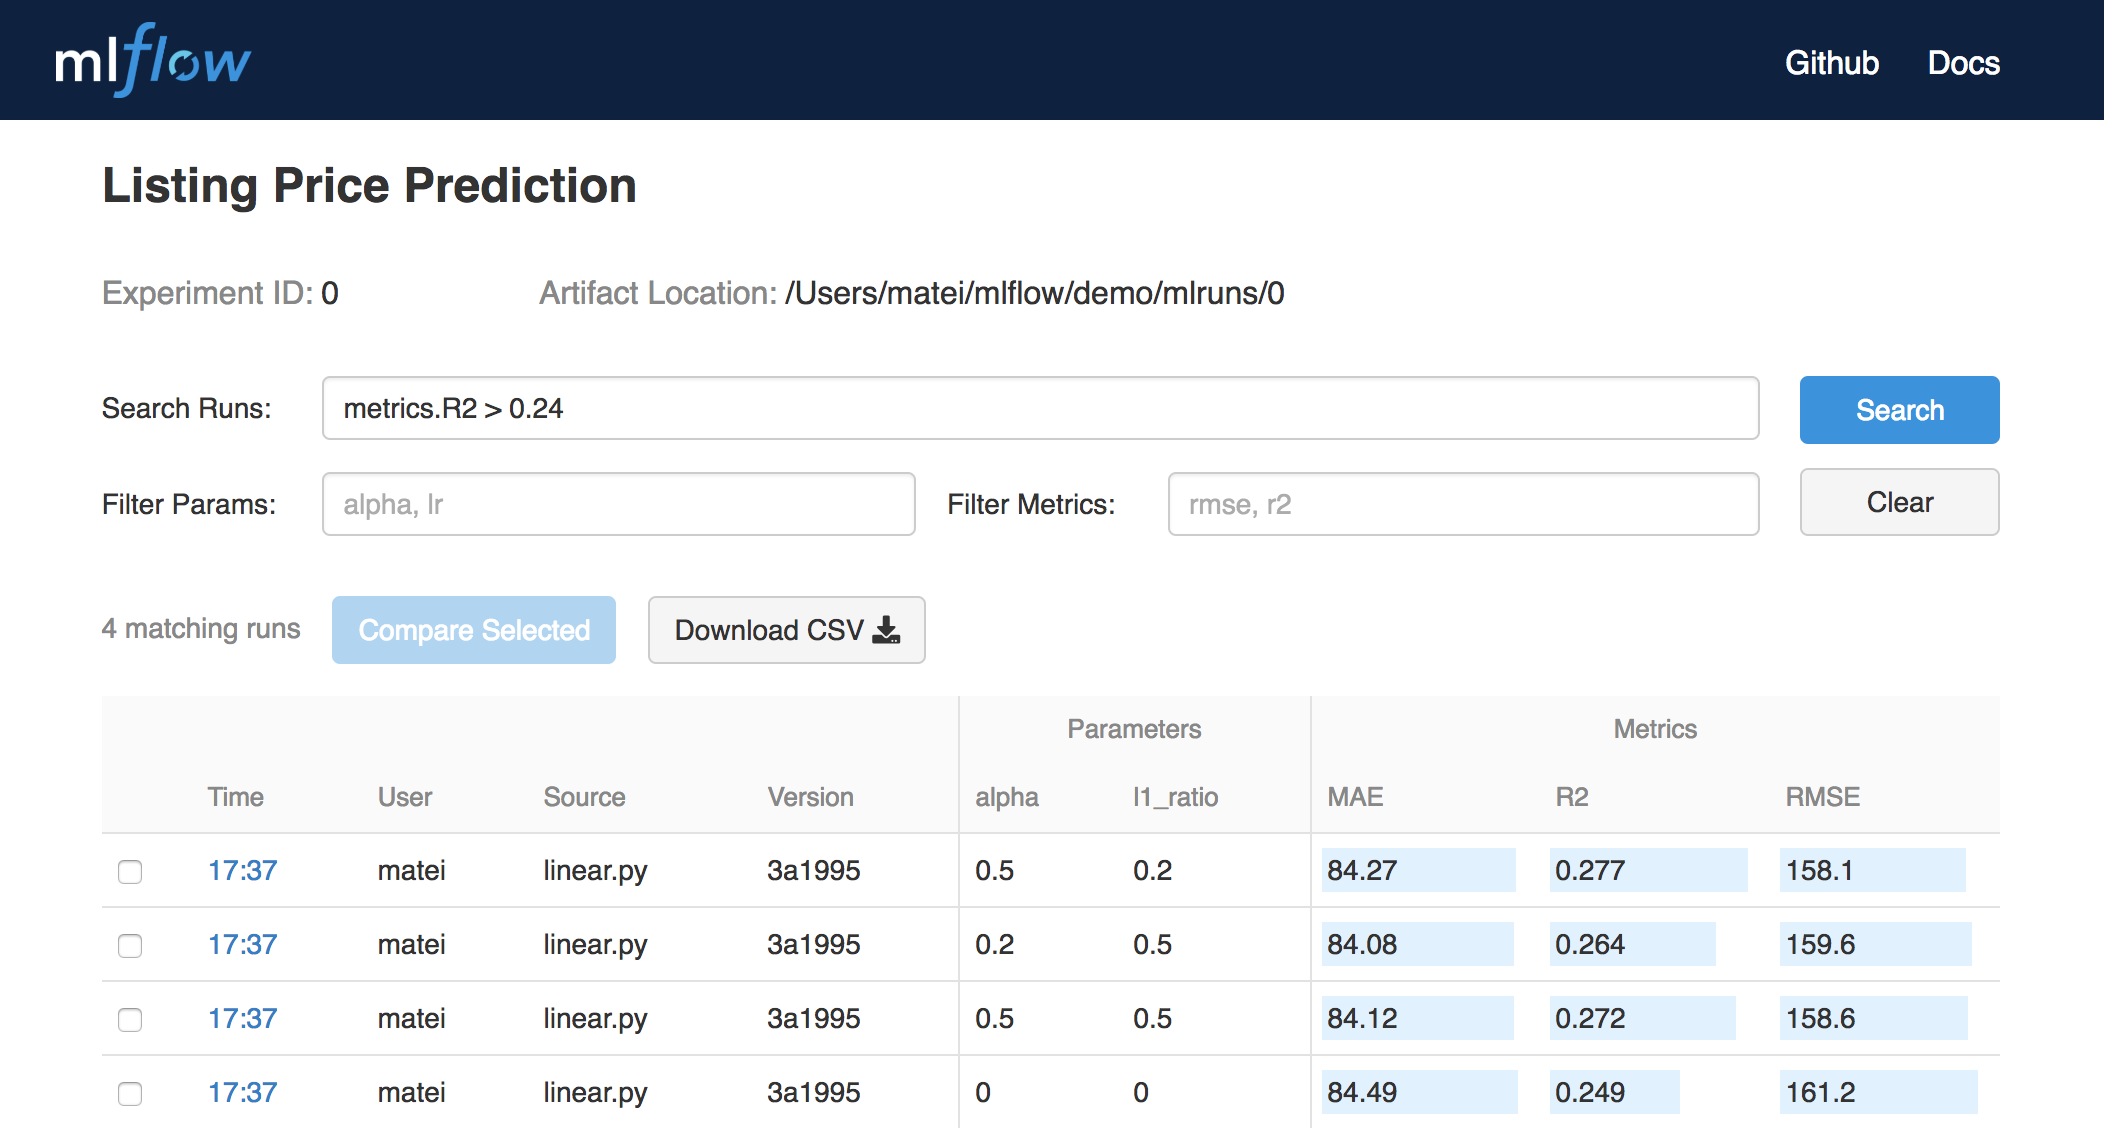
\includegraphics[bb=0 0 1052 564,width=\textwidth]{tracking.png}
\caption{MLflow Tracking UI showing several runs in an experiment. Clicking each run lists its metrics, artifacts and output details and lets the user post comments about the run.}
\label{fig:tracking-ui}
\end{figure}

\subsection{MLflow Projects}

MLflow Projects provide a simple format for packaging reproducible data science code. Each project is simply a directory with code or a Git repository, and uses a descriptor file to specify its dependencies and how to run the code. A MLflow Project is defined by a simple YAML file called MLproject, as shown below:

\begin{Verbatim}[frame=single,fontsize=\small,samepage=true]
name: My Project
conda_env: conda.yaml
entry_points:
  main:
    parameters:
      data_file: path
      alpha: {type: float, default: 0.1}
    command: "python train.py --reg-param {alpha} --data {data_file}"
\end{Verbatim}


Projects can specify their dependencies through a Conda environment or (in an upcoming release) a Docker container specification. A project may also have multiple entry points for invoking runs, with named parameters that downstream users can provide without understanding the internals of the project.

Users can run projects using the \texttt{mlflow run} command line tool, either from local files or a Git repository:

\begin{Verbatim}[frame=single,fontsize=\small,samepage=true]
mlflow run git@github.com:databricks/mlflow-example.git -P alpha=0.5
\end{Verbatim}

Alternatively, projects can be called programmatically using MLflow's API. This can be used to implement multi-step workflows or to pass projects a ``black box'' into automated tools such as hyperparameter search~\cite{hyperopt}.

In either case, MLflow will automatically set up the project's runtime environment and execute it. If the code inside the project uses the MLflow Tracking API, MLflow will also remember the project version executed (that is, the Git commit) and show an \texttt{mlflow run} command to re-execute it in its UI. Finally, MLflow projects can also be submitted to cloud platforms such as Databricks for remote execution.

\subsection{MLflow Models}

MLflow Models are a convention for packaging machine learning models in multiple formats called ``flavors'', allowing diverse tools to understand the model at different levels of abstractions. MLflow also offers a variety of built-in tools to deploy models in its standard favors. For example, the same model can be deployed as a Docker container for REST serving, as an Apache Spark user-defined function (UDF) for batch inference, or into cloud-managed serving platforms like Amazon SageMaker and Azure ML.

Each MLflow Model is simply stored as a directory containing arbitrary files and an MLmodel YAML file that lists the flavors it can be used in and additional metadata about how it was created:

\begin{Verbatim}[frame=single,fontsize=\small,samepage=true]
time_created: 2018-02-21T13:21:34.12
run_id: c4b65fc2c57f4b6d80c6e58a9dcb9f01
flavors:
  sklearn:
    sklearn_version: 0.19.1
    pickled_model: model.pkl
  python_function:
    loader_module: mlflow.sklearn
    pickled_model: model.pkl
\end{Verbatim}

In this example, the model can be used with tools that support either the \texttt{sklearn} or \texttt{python\_function} model flavors. For example, the MLflow SciKit-Learn library knows how to load a \texttt{sklearn} model as a SciKit-Learn Python object, but other deployment tools, such as running the model in a Docker HTTP server, only understand lower-level flavors like \texttt{python\_function}.
In addition, models logged using MLflow Tracking APIs will automatically include a reference to that run's unique ID, letting users discover how they were built.

\section{Example Use Cases}

In this section, we describe three sample MLflow use cases to highlight how users can leverage each component.

\vspace{-0.6em}
\paragraph{Experiment tracking.} A European energy company is using MLflow to track and update hundreds of energy grid models. This team's goal is to build a time series model for every major energy producer (e.g., power plant) and consumer (e.g., factory), monitor these using standard metrics, and combine the predictions to drive business processes such as pricing. Because a single team is responsible for hundreds of models, possibly using different ML libraries, it was important to have a standard development and tracking process. The team has standardized on using Jupyter notebooks for development, MLflow Tracking for metrics, and Databricks jobs for inference.

\vspace{-0.6em}
\paragraph{Reproducible projects.} An online marketplace is using MLflow Projects to package deep learning jobs using Keras and run them in the cloud. Each data scientist develops models locally on his or her laptop using a small dataset, checks them into a Git repository with an MLproject file, and submits remote runs of the project to GPU instances in the cloud for large-scale training or hyperparameter search. Using MLflow Projects makes it easy to create the same software environment in the cloud and share project code between different data scientists.

\vspace{-0.6em}
\paragraph{Model packaging.} The data science team at an e-commerce site is using MLflow Models to package recommendation models for use by application engineers. The technical challenge here was that the recommendation application includes both a standard, ``off-the-shelf'' recommendation model and custom business logic for pre- and post-processing. For example, the application might include custom code to make sure that the recommended items are diverse. This business logic needs to change in sync with the model, and the data science team wants to control both the business logic and the model, without having to submit a patch to the web application each time this logic has to change.
Moreover, the team wants to A/B test distinct models with distinct versions of the processing logic.
The solution was to package both the recommendation model and the custom logic using the \texttt{python\_function} flavor in an MLflow Model, which can then be deployed and tested as a single unit. %This allows production engineers to deploy the recommendation code as they please without the processing logic falling out of sync with the model.

\section{Related Work}

Many software systems aim to simplify ML development.
The closest to our work are the end-to-end ``ML platforms'' at large web companies.
For example, Facebook's FBLearner lets users write reusable workflow steps that run over data in Apache Hive~\cite{fblearner};
Uber's Michelangelo gives users a toolkit of algorithms to choose from that it can automatically train and deploy~\cite{michelangelo}; and Google's TFX provides data preparation and serving tools around TensorFlow~\cite{tfx}.
Anecdotally, these platforms greatly accelerate ML development, showing the benefits of standardizing the ML lifecycle.
However, they generally restrict users to a specific set of algorithms or libraries, so teams are on their own when they step outside these boundaries.
Our goal in MLflow is to let users easily bring their own tools and software in as many steps in the process as possible through our ``open interface'' design.
This includes custom training steps, inference code, and logged parameters and artifacts.

Other systems also tackle specific problems within the ML lifecycle. For example, Sacred~\cite{sacred}, ModelDB~\cite{modeldb} and TensorBoard~\cite{tensorboard} let users track experiments; PMML~\cite{pmml} and ONNX~\cite{onnx} are cross-library model serialization formats; Clipper~\cite{clipper} can deploy arbitrary models as Docker containers; and CDE~\cite{cde}, CodaLab~\cite{codalab}, Binder~\cite{binder} and Repo2Docker~\cite{repo2docker} enable reproducible software runs. MLflow combines these concepts with new ones, such as multi-flavor model packaging, into a unified system design and API.

\section{Conclusion}

For machine learning to have widespread commercial impact, organizations require the same kinds of reliable engineering processes around ML that exist in other engineering disciplines such as software development. In this paper, we have described some of the key challenges that differentiate ML development from traditional software development, such as experimentation, reproducibility, and reliable production deployment. We have also described MLflow, a software platform that can structure the machine learning lifecycle while giving users broad flexibility to use their own ML algorithms, software libraries and development processes.
MLflow is available as open source software at \url{https://www.mlflow.org}.


{\small

\begin{thebibliography}{10}

  \bibitem{abadi2016tensorflow}
  M.~Abadi, P.~Barham, J.~Chen, Z.~Chen, A.~Davis, J.~Dean, M.~Devin,
    S.~Ghemawat, G.~Irving, M.~Isard, et~al.
  \newblock {TensorFlow: A System for Large-Scale Machine Learning}.
  \newblock In {\em OSDI}, volume~16, pages 265--283, 2016.

  \bibitem{tfx}
  D.~Baylor, E.~Breck, H.-T. Cheng, N.~Fiedel, C.~Y. Foo, Z.~Haque, S.~Haykal,
    M.~Ispir, V.~Jain, L.~Koc, C.~Y. Koo, L.~Lew, C.~Mewald, A.~N. Modi,
    N.~Polyzotis, S.~Ramesh, S.~Roy, S.~E. Whang, M.~Wicke, J.~Wilkiewicz,
    X.~Zhang, and M.~Zinkevich.
  \newblock Tfx: A tensorflow-based production-scale machine learning platform.
  \newblock In {\em Proceedings of the 23rd ACM SIGKDD International Conference
    on Knowledge Discovery and Data Mining}, KDD '17, pages 1387--1395, New York,
    NY, USA, 2017. ACM.

  \bibitem{hyperopt}
  J.~Bergstra, B.~Komer, C.~Eliasmith, D.~Yamins, and D.~D. Cox.
  \newblock Hyperopt: a python library for model selection and hyperparameter
    optimization.
  \newblock {\em Computational Science and Discovery}, 8(1):014008, 2015.

  \bibitem{binder}
  {Binder}.
  \newblock \url{https://mybinder.org}, 2018.

  \bibitem{clipper}
  D.~Crankshaw, X.~Wang, G.~Zhou, M.~J. Franklin, J.~E. Gonzalez, and I.~Stoica.
  \newblock Clipper: A low-latency online prediction serving system.
  \newblock In {\em Proceedings of the 14th USENIX Conference on Networked
    Systems Design and Implementation}, NSDI'17, pages 613--627, Berkeley, CA,
    USA, 2017. USENIX Association.

  \bibitem{fblearner}
  J.~Dunn.
  \newblock Introducing {FBLearner Flow}: Facebook’s {AI} backbone.
  \newblock
    \url{https://code.fb.com/core-data/introducing-fblearner-flow-facebook-s-ai-backbone/}.

  \bibitem{repo2docker}
  J.~Forde, T.~Head, C.~Holdgraf, Y.~Panda, G.~Nalvarte, M.~Pacer, F.~Perez,
    B.~Ragan-Kelley, and E.~Sundell.
  \newblock Reproducible research environments with repo2docker.
  \newblock ICML, 07/2018 2018.

  \bibitem{tensorboard}
  Google.
  \newblock Tensorboard: Visualizing learning.
  \newblock \url{https://www.tensorflow.org/guide/summaries_and_tensorboard}.

  \bibitem{pmml}
  A.~Guazzelli, W.-C. Lin, and T.~Jena.
  \newblock {\em PMML in Action: Unleashing the Power of Open Standards for Data
    Mining and Predictive Analytics}.
  \newblock CreateSpace, Paramount, CA, 2nd edition, 2012.

  \bibitem{cde}
  P.~J. Guo.
  \newblock {CDE}: A tool for creating portable experimental software packages.
  \newblock {\em Computing in Science and Engineering}, 14(4):32--35, 2012.

  \bibitem{michelangelo}
  J.~Hermann and M.~D. Balso.
  \newblock Meet {Michelangelo}: Uber’s machine learning platform.
  \newblock \url{https://eng.uber.com/michelangelo/}.

  \bibitem{sacred}
  {K}laus {G}reff, {A}aron {K}lein, {M}artin {C}hovanec, {F}rank {H}utter, and
    {J}\"urgen {S}chmidhuber.
  \newblock {T}he {S}acred {I}nfrastructure for {C}omputational {R}esearch.
  \newblock In {K}aty {H}uff, {D}avid {L}ippa, {D}illon {N}iederhut, and
    M.~{P}acer, editors, {\em {P}roceedings of the 16th {P}ython in {S}cience
    {C}onference}, pages 49 -- 56, 2017.

  \bibitem{codalab}
  P.~Liang et~al.
  \newblock {CodaLab}.
  \newblock \url{https://worksheets.codalab.org}, 2018.

  \bibitem{onnx}
  {ONNX Group}.
  \newblock {ONNX}.
  \newblock \url{https://onnx.ai}.

  \bibitem{modeldb}
  M.~Vartak, H.~Subramanyam, W.-E. Lee, S.~Viswanathan, S.~Husnoo, S.~Madden, and
    M.~Zaharia.
  \newblock Modeldb: A system for machine learning model management.
  \newblock In {\em Proceedings of the Workshop on Human-In-the-Loop Data
    Analytics}, HILDA '16, pages 14:1--14:3, New York, NY, USA, 2016. ACM.

  \end{thebibliography}


}
%\bibliographystyle{abbrv}
%\bibliography{paper}

\end{document}
\end{article}.
% The string NAME given in \begin{articlesection}{NAME} is the topic of
% the special issue, and results in the title ``Special Issue on NAME''
% as the title for the article section on the cover page.
%
%%%%%%%%%%%%%%%%%%%%%%%%%%%%%%%%%%%%%%%%%%%%%%%%%%%%%%%%%%%%%%%%%%%%%%%%%%

\newenvironment{articlesection}[1]%
       {\clearpage
	\tocskip{\bigskipamount}
	\tocrule
	\tocheading{\strut Special Issue on #1}
%	\tocrule
	\tocskip{\smallskipamount}
	}%
       {\clearpage}
\newenvironment{article}[2]
       {\clearpage
	\newcommand{\articletitle}{#1}
	\newcommand{\articleauthor}{#2}
	\tocsubentry{\articletitle}{\articleauthor}
	\pageheading{\articleauthor}{\articletitle}
	\thispagestyle{plain}
	\makeatletter
        \@RestoreMaketitle
	\@UndefinePreambleCommands
	\NeedsTeXFormat{LaTeX2e}
\ProvidesPackage{deauthor}[2002/04/01 Data Engineering Bulletin Author package]

%
% Undefine the \date command, so no date is printed with the title
%
\renewcommand{\date}[1]{}
\renewcommand{\@date}{\@empty}

%
% Undefine the titlepage environment so that articles don't try to
% circumvent the journal's formatting conventions for the first page.
% This works for the article class, but causes trouble for reports and 
% books since the \maketitle command is defined in terms of the titlepage 
% environment.
%
\renewenvironment{titlepage}{}{}

%
% Undefine the \pagestyle and \thispagestyle commands so that articles
% don't try to change the page style.
%
\renewcommand{\pagestyle}[1]{}
\renewcommand{\thispagestyle}[1]{}

%
% Define common theorem-like environment created with the \newtheorem
% command.  First we have to undefine them all since we just defined them
% in the previous article.  Also, define a proof environment and a \qed
% symbol to end the proof.
%
% This initial hack redefines the theorem-like environments of latex to
% follow the theorem heading with a colon (e.g. Theorem 4:) and print
% the theorem text in roman font.
%
\renewcommand{\@begintheorem}[2]%
        {\trivlist \item[\hskip \labelsep{\bf #1\ #2:}]}
\renewcommand{\@opargbegintheorem}[3]%
        {\trivlist \item[\hskip \labelsep{\bf #1\ #2\ (#3):}]}
%
\let\theorem\relax
\let\lemma\relax
\let\corollary\relax
\let\proposition\relax
\let\claim\relax
\let\definition\relax
\let\proof\relax \let\endproof\relax
%
\newtheorem{theorem}{Theorem}
\newtheorem{lemma}[theorem]{Lemma}
\newtheorem{corollary}[theorem]{Corollary}
\newtheorem{proposition}[theorem]{Proposition}
\newtheorem{claim}[theorem]{Claim}
\newtheorem{definition}[theorem]{Definition}
%
\newenvironment{proof}{\noindent {\bf Proof:}}{}
\newcommand{\squarebox}[1]{\hbox to #1{\hfill\vbox to #1{\vfill}}}
\newcommand{\qed}{\hspace*{\fill}
            \vbox{\hrule\hbox{\vrule\squarebox{.667em}\vrule}\hrule}\smallskip}

%
% Define an example environment, just another theorem environment but with
% independent numbering.
%
\let\example\relax
\newtheorem{example}{Example}

%
% Define an indented abstract environment.
%
\renewenvironment{abstract}%
  {\begin{center}\textbf{Abstract}\end{center}\narrower\itshape}%
  {\par}  

% 
% Reset all section and figure counters so that an article's section
% and figure numbers begin with 1.
%
\setcounter{section}{0}
\setcounter{figure}{0}
\setcounter{table}{0}


%
% Place page formatting parameters (like page dimensions) here
% These should match the dimensions in bulletin.sty.
%
\textheight     9.0in
\textwidth      6.75in
\oddsidemargin  0.0in
\evensidemargin -0.25in
\topmargin      0.0in
\headheight     0.0in
\headsep        0.0in
%\footheight     0.0in

\@twosidetrue        % print on two sides of a page

%
% Authors are not supposed to change page dimensions.
%

\let\@setlength\setlength       % save old definition
\renewcommand{\setlength}[2]{%
  \@VerifyChangeableLength{#1}%
  \if@ChangeableLength\@setlength{#1}{#2}\else\@UnchangeableError{#1}\fi}

\let\@addtolength\addtolength   % save old definition
\renewcommand{\addtolength}[2]{%
  \@VerifyChangeableLength{#1}%
  \if@ChangeableLength\@addtolength{#1}{#2}\else\@UnchangeableError{#1}\fi}

\let\@settowidth\settowidth     % save old definition
\renewcommand{\settowidth}[2]{%
  \@VerifyChangeableLength{#1}%
  \if@ChangeableLength\@settowidth{#1}{#2}\else\@UnchangeableError{#1}\fi}

\newif\if@ChangeableLength      \@ChangeableLengthtrue
\newcommand{\@VerifyChangeableLength}[1]{%
  \ifx#1\textwidth              \@ChangeableLengthfalse
  \else\ifx#1\textheight        \@ChangeableLengthfalse
  \else\ifx#1\textwidth         \@ChangeableLengthfalse
  \else\ifx#1\oddsidemargin     \@ChangeableLengthfalse
  \else\ifx#1\evensidemargin    \@ChangeableLengthfalse
  \else\ifx#1\topmargin         \@ChangeableLengthfalse
  \else\ifx#1\headheight        \@ChangeableLengthfalse
  \else\ifx#1\headsep           \@ChangeableLengthfalse
  \else\ifx#1\footheight        \@ChangeableLengthfalse
  \else\@ChangeableLengthtrue\fi\fi\fi\fi\fi\fi\fi\fi\fi}
\newcommand{\@UnchangeableError}[1]{%
  \errmessage{Error: Authors are not allowed to change #1.. Ignored}}

%
% We want the title to be typeset in boldface, and the author names
% to be typeset in italics.  We can hardwire this for the title,
% but trying to do the same thing for the author causes confusion
% due to the use of \@author in \@maketitle in article.sty.
% 
% We also want to print a copyright notice and the bulletin title at
% the bottom of every first page.
%
\renewcommand{\title}[1]{%
  \gdef\@title{\textbf{#1}}
  \begingroup 
  \renewcommand{\thefootnote}{\fnsymbol{footnote}}
  \global\setcounter{footnote}{0}
  \footnotetext{%
    \emph{Copyright {\@BulletinYear} IEEE. Personal use of this material is
    permitted. However, permission to reprint/republish this material for
    advertising or promotional purposes or for creating new collective
    works for resale or redistribution to servers or lists, or to reuse
    any copyrighted component of this work in other works must be obtained
    from the IEEE.}\\
    \textbf{Bulletin of the IEEE Computer Society Technical Committee on
    Data Engineering} \\
    \footnoterule
  }%
  \endgroup
}
\providecommand{\@BulletinYear}{0000}
\providecommand{\bulletinyear}[1]{\renewcommand{\@BulletinYear}{#1}}

  % read in the author style file
	\makeatother
       }%
       {\clearpage}

%%%%%%%%%%%%%%%%%%%%%%%%%%%%%%%%%%%%%%%%%%%%%%%%%%%%%%%%%%%%%%%%%%%%%%%%%%
%
%  CONFERENCE NOTICES SECTION
%
% The section is enclosed between \begin{callsection} and 
% \end{callssection} commands, and each call for papers is enclosed between 
% \begin{call}{NAME} and \end{call} commands where
% NAME is the name of the conference.
%
%%%%%%%%%%%%%%%%%%%%%%%%%%%%%%%%%%%%%%%%%%%%%%%%%%%%%%%%%%%%%%%%%%%%%%%%%%

\newenvironment{callsection}%
       {\clearpage
	\tocskip{\bigskipamount}
	\tocrule
	\tocheading{\strut Conference and Journal Notices}
	\tocskip{\smallskipamount}
	}%
       {\clearpage}
\newenvironment{call}[1]
       {\clearpage
	\newcommand{\calltitle}{#1}
	\tocsubentry{\calltitle}{}
	\pageheading{\calltitle}{\calltitle}
	\thispagestyle{plain}
	\makeatletter
        \@RestoreMaketitle
	\@UndefinePreambleCommands
	\NeedsTeXFormat{LaTeX2e}
\ProvidesPackage{deauthor}[2002/04/01 Data Engineering Bulletin Author package]

%
% Undefine the \date command, so no date is printed with the title
%
\renewcommand{\date}[1]{}
\renewcommand{\@date}{\@empty}

%
% Undefine the titlepage environment so that articles don't try to
% circumvent the journal's formatting conventions for the first page.
% This works for the article class, but causes trouble for reports and 
% books since the \maketitle command is defined in terms of the titlepage 
% environment.
%
\renewenvironment{titlepage}{}{}

%
% Undefine the \pagestyle and \thispagestyle commands so that articles
% don't try to change the page style.
%
\renewcommand{\pagestyle}[1]{}
\renewcommand{\thispagestyle}[1]{}

%
% Define common theorem-like environment created with the \newtheorem
% command.  First we have to undefine them all since we just defined them
% in the previous article.  Also, define a proof environment and a \qed
% symbol to end the proof.
%
% This initial hack redefines the theorem-like environments of latex to
% follow the theorem heading with a colon (e.g. Theorem 4:) and print
% the theorem text in roman font.
%
\renewcommand{\@begintheorem}[2]%
        {\trivlist \item[\hskip \labelsep{\bf #1\ #2:}]}
\renewcommand{\@opargbegintheorem}[3]%
        {\trivlist \item[\hskip \labelsep{\bf #1\ #2\ (#3):}]}
%
\let\theorem\relax
\let\lemma\relax
\let\corollary\relax
\let\proposition\relax
\let\claim\relax
\let\definition\relax
\let\proof\relax \let\endproof\relax
%
\newtheorem{theorem}{Theorem}
\newtheorem{lemma}[theorem]{Lemma}
\newtheorem{corollary}[theorem]{Corollary}
\newtheorem{proposition}[theorem]{Proposition}
\newtheorem{claim}[theorem]{Claim}
\newtheorem{definition}[theorem]{Definition}
%
\newenvironment{proof}{\noindent {\bf Proof:}}{}
\newcommand{\squarebox}[1]{\hbox to #1{\hfill\vbox to #1{\vfill}}}
\newcommand{\qed}{\hspace*{\fill}
            \vbox{\hrule\hbox{\vrule\squarebox{.667em}\vrule}\hrule}\smallskip}

%
% Define an example environment, just another theorem environment but with
% independent numbering.
%
\let\example\relax
\newtheorem{example}{Example}

%
% Define an indented abstract environment.
%
\renewenvironment{abstract}%
  {\begin{center}\textbf{Abstract}\end{center}\narrower\itshape}%
  {\par}  

% 
% Reset all section and figure counters so that an article's section
% and figure numbers begin with 1.
%
\setcounter{section}{0}
\setcounter{figure}{0}
\setcounter{table}{0}


%
% Place page formatting parameters (like page dimensions) here
% These should match the dimensions in bulletin.sty.
%
\textheight     9.0in
\textwidth      6.75in
\oddsidemargin  0.0in
\evensidemargin -0.25in
\topmargin      0.0in
\headheight     0.0in
\headsep        0.0in
%\footheight     0.0in

\@twosidetrue        % print on two sides of a page

%
% Authors are not supposed to change page dimensions.
%

\let\@setlength\setlength       % save old definition
\renewcommand{\setlength}[2]{%
  \@VerifyChangeableLength{#1}%
  \if@ChangeableLength\@setlength{#1}{#2}\else\@UnchangeableError{#1}\fi}

\let\@addtolength\addtolength   % save old definition
\renewcommand{\addtolength}[2]{%
  \@VerifyChangeableLength{#1}%
  \if@ChangeableLength\@addtolength{#1}{#2}\else\@UnchangeableError{#1}\fi}

\let\@settowidth\settowidth     % save old definition
\renewcommand{\settowidth}[2]{%
  \@VerifyChangeableLength{#1}%
  \if@ChangeableLength\@settowidth{#1}{#2}\else\@UnchangeableError{#1}\fi}

\newif\if@ChangeableLength      \@ChangeableLengthtrue
\newcommand{\@VerifyChangeableLength}[1]{%
  \ifx#1\textwidth              \@ChangeableLengthfalse
  \else\ifx#1\textheight        \@ChangeableLengthfalse
  \else\ifx#1\textwidth         \@ChangeableLengthfalse
  \else\ifx#1\oddsidemargin     \@ChangeableLengthfalse
  \else\ifx#1\evensidemargin    \@ChangeableLengthfalse
  \else\ifx#1\topmargin         \@ChangeableLengthfalse
  \else\ifx#1\headheight        \@ChangeableLengthfalse
  \else\ifx#1\headsep           \@ChangeableLengthfalse
  \else\ifx#1\footheight        \@ChangeableLengthfalse
  \else\@ChangeableLengthtrue\fi\fi\fi\fi\fi\fi\fi\fi\fi}
\newcommand{\@UnchangeableError}[1]{%
  \errmessage{Error: Authors are not allowed to change #1.. Ignored}}

%
% We want the title to be typeset in boldface, and the author names
% to be typeset in italics.  We can hardwire this for the title,
% but trying to do the same thing for the author causes confusion
% due to the use of \@author in \@maketitle in article.sty.
% 
% We also want to print a copyright notice and the bulletin title at
% the bottom of every first page.
%
\renewcommand{\title}[1]{%
  \gdef\@title{\textbf{#1}}
  \begingroup 
  \renewcommand{\thefootnote}{\fnsymbol{footnote}}
  \global\setcounter{footnote}{0}
  \footnotetext{%
    \emph{Copyright {\@BulletinYear} IEEE. Personal use of this material is
    permitted. However, permission to reprint/republish this material for
    advertising or promotional purposes or for creating new collective
    works for resale or redistribution to servers or lists, or to reuse
    any copyrighted component of this work in other works must be obtained
    from the IEEE.}\\
    \textbf{Bulletin of the IEEE Computer Society Technical Committee on
    Data Engineering} \\
    \footnoterule
  }%
  \endgroup
}
\providecommand{\@BulletinYear}{0000}
\providecommand{\bulletinyear}[1]{\renewcommand{\@BulletinYear}{#1}}

  % read in the author style file
	\makeatother
	}%
       {\clearpage}

%%%%%%%%%%%%%%%%%%%%%%%%%%%%%%%%%%%%%%%%%%%%%%%%%%%%%%%%%%%%%%%%%%%%%%%%%%
%
%  Special Sections
%
% This does nothing but insert a heading in the table of contents and a 
% heading in the text.  This was requested, but I'm not sure what this 
% environment is going to be used for.  This is basically just a 
% demonstration that sections parameterized by the section title are possible.
%
%%%%%%%%%%%%%%%%%%%%%%%%%%%%%%%%%%%%%%%%%%%%%%%%%%%%%%%%%%%%%%%%%%%%%%%%%%
\newenvironment{specialsection}[1]%
       {\clearpage
	\heading{#1}
	\tocskip{\bigskipamount}
	\tocheading{\strut #1}
	\tocskip{\smallskipamount}
	}%
       {\clearpage}

%%%%%%%%%%%%%%%%%%%%%%%%%%%%%%%%%%%%%%%%%%%%%%%%%%%%%%%%%%%%%%%%
%%%%%%%%%%%%%%%%%%%%%%%%%%%%%%%%%%%%%%%%%%%%%%%%%%%%%%%%%%%%%%%%
%%
%% Table of Contents
%%
%% This is the hardest part of the style file.  The following
%% commands are used to generate the table of contents on the front
%% cover.  Most of the table of contents will be generated automatically
%% by environments like the letter and article environments below, but
%% the editor will want to insert some lines into the table of contents
%% by hand.  The following commands are provided:
%% 
%% \tocrule: 
%%   to generate a solid line to separate sections of the TOC
%% \tocskip{SKIP}:
%%   to insert a vertical skip of SKIP as in \tocskip{1in}
%% \tocheading{TITLE}: 
%% \tocsubheading{TITLE}: 
%% \tocsubsubheading{TITLE}: 
%%   to generate a section heading in the TOC, and more generally to 
%%   insert an arbitrary paragraph of text into the TOC.  Subheadings
%%   and subsubheadings are indented by \tocindention.
%% \tocentry{TITLE}{AUTHOR}:
%% \tocsubentry{TITLE}{AUTHOR}:
%% \tocsubsubentry{TITLE}{AUTHOR}:
%%   to generate an entry of the form ``AUTHOR .... TITLE page'' in the
%%   TOC for something like an article, etc, where page is the current 
%%   page number.  Again, subentries and subsubentries are indented.
%% 
%% There are also some lower level commands used to implement these command,
%% but an editor should never have to use them.
%% 
%% ONE CAVEAT: The arguments to all these commands are moving
%% arguments, so you must \protect fragile commands like \bigskip
%% and \Large.  (See \protect in the LaTeX book.)  Use 
%% \tocheading{\protect\bigskip\protect\Huge Introduction} and not
%% \tocheading{\bigskip\Huge Introduction}
%% 

%
% \tocrule generates a solid line across the table of contents,
% useful for physically dividing the table of contents into sections
%
\newcommand{\tocrule}%
  {\addtocontents{toc}{\protect\smallskip\hrule\protect\smallskip}}

%
% \tocskip{SKIP} adds SKIP vertical space to the table of contents.
%
\newcommand{\tocskip}[1]{\addtocontents{toc}{\vskip #1}}

%
% \tocheading{TITLE} generates a table of contents section heading
% TITLE without a page number, and \tocsubheading and \tocsubsubheading
% are similar.  It is intended to be used to generate headings for 
% sections in the table of contents, headings such as ``Letters to 
% the Editor'' or ``Contributed Articles'' or ``Calls for Papers''.
%
\newcommand{\tocheading}[1]{%
	\@TocWrite{0}{\@FormatTocHeading{\protect\textbf{\Large #1}}}}
\newcommand{\tocsubheading}[1]{%
	\@TocWrite{1}{\@FormatTocHeading{\protect\large #1}}}
\newcommand{\tocsubsubheading}[1]{%
	\@TocWrite{2}{\@FormatTocHeading{\normalsize #1}}}

%
% \tocentry{TITLE}{AUTHOR} generates a table of contents entry for
% a contribution with TITLE and AUTHOR, either of which may be empty,
% and a page number, and \tocsubentry and \tocsubsubentry are similar.
% These commands are intended for use with \tocheading, etc., for structuring
% the table of contents.  For example, in an special issue the preface 
% letters from the journal editor and special issue editor might be 
% presented in an introduction section.  The introduction toc heading
% would be generated with \tocheading{Introduction}, and the toc entries for
% the two letters would be generated by 
% \tocsubentry{Special Issue Greetings}{Editor S. Issue} and
% \tocsubentry{My Thanks to Editor S. Issue}{Journal Editor}.
%
\newcommand{\tocentry}[2]{%
	\@TocWrite{0}{\@FormatTocEntry{#1}{#2}{\thepage}}}
\newcommand{\tocsubentry}[2]{%
	\@TocWrite{1}{\@FormatTocEntry{#1}{#2}{\thepage}}}
\newcommand{\tocsubsubentry}[2]{%
	\@TocWrite{2}{\@FormatTocEntry{#1}{#2}{\thepage}}}

%
% Now begin the low level commands that the editor should never have to use.
%

%
% \@TocWrite{LEVEL}{LINE} writes to the table of contents a (typically
% preformatted) entry LINE, after indenting the entry appropriately.
% The LEVEL is an integer 0, 1, 2, ... and gives the number of times
% that LINE should be indented by an amount given by \tocindention.
%
% This macro is tricky: it must indent all lines but the first by
% \toclhindent on the left, and it must indent all lines but the last
% by \tocrhindent on the left.  For example, an entry for an article
% with title TTT... and author AAA... and page number PPP must be typeset 
% like
% 
% TTTTTTTTTTTTTTTTTTTTTTTTTTTTTTTTTTTTTT
%     TTTTTTTTTTTT......................
%     ........................AAAAAAAAAA  PPP
% 
\newcommand{\@TocWrite}[2]{%
	\addtocontents{toc}{\vbox{\strut\hbox to \hsize{%
	\hskip #1\tocindention 
  	\begingroup
	\advance \hsize by -#1\tocindention
	\hbox to \hsize{\vbox{%
	\leftskip     \toclhindent
  	\parindent   -\toclhindent
  	\rightskip    \tocrhindent
  	\parfillskip -\tocrhindent
	#2}}\endgroup}\strut}}}

%
% \@FormatTocEntry{TITLE}{AUTHOR}{PAGE} formats the TITLE, AUTHOR, and 
% PAGE number of what will be a table of contents entry or section heading,
% and any of the arguments may be empty.  This does not actually write
% to the table of contents itself, and does not indent entries and section
% headings appropriately.  It is meant to be used with \outputtocentry.
% The width given by \tocpagenumwidth is the width of the box in which
% page numbers are typeset.
% 
% This macro is tricky: it must compute on its own whether there is enough
% space for both the title and author/page number on the same line.  If
% not, it must split the line between the title and the author/page
% number.  (See the example above under \@TocWrite.)
% The basic idea comes from the TeXbook on page 106.  The macro
% works as long as the list of authors does not require more than two
% complete lines of text to print (the title can be as long as you like).
% When the macro breaks, the author/page number is not flush right on the
% page.  I don't understand linebreaking enough to debug this.
%
\newcommand{\@FormatTocEntry}[3]{%
  #1\unskip\nobreak\@DotFill\penalty50\@DotLeaders\hskip1em\nobreak
  \hbox{}\@DotFill{\it #2\/}\nobreak\hbox to\tocpagenumwidth{\hss #3}}
\newcommand{\@DotLeaders}{\xleaders\hbox to .5em{\hss.\hss}}
\newcommand{\@DotFill}{\@DotLeaders\hfill}

%
% \@FormatTocHeading{TITLE} formats the TITLE of what will be a tocheading.
%
\newcommand{\@FormatTocHeading}[1]{#1\hfil\hbox{}}

%
% Redefine \contentsname to null to avoid printing ``Contents'' on front 
% cover.  This might not interact well with book and report classes.
%
\renewcommand{\tableofcontents}{\@starttoc{toc}}

%
% Set tocdepth so that the \section-like commands do not generate 
% Table of Contents entries.  We set tocdepth to -2 since section 
% levels are usually defined to be -1, 0, 1, ... or 0, 1, 2, ....
%
\setcounter{tocdepth}{-2}

%%%%%%%%%%%%%%%%%%%%%%%%%%%%%%%%%%%%%%%%%%%%%%%%%%%%%%%%%%%%%%%%
%%%%%%%%%%%%%%%%%%%%%%%%%%%%%%%%%%%%%%%%%%%%%%%%%%%%%%%%%%%%%%%%
%%
%% Headings
%%
%%%%%%%%%%%%%%%%%%%%%%%%%%%%%%%%%%%%%%%%%%%%%%%%%%%%%%%%%%%%%%%%
%%%%%%%%%%%%%%%%%%%%%%%%%%%%%%%%%%%%%%%%%%%%%%%%%%%%%%%%%%%%%%%%
%
% A heading in the bulletin is like a section in an article.
% The commands \heading, \subheading, and \subsubheading generate headings
% for the sections.  Unlike the \section command in the normal 
% document styles, the \heading commands does not automatically 
% generate a line in the table of contents.  You must do this 
% explicitly if you want one.
%
\newcommand{\heading}{\section*}
\newcommand{\subheading}{\subsection*}
\newcommand{\subsubheading}{\subsubsection*}

%%%%%%%%%%%%%%%%%%%%%%%%%%%%%%%%%%%%%%%%%%%%%%%%%%%%%%%%%%%%%%%%
%%%%%%%%%%%%%%%%%%%%%%%%%%%%%%%%%%%%%%%%%%%%%%%%%%%%%%%%%%%%%%%%
%%
%% Pageheadings
%%
%%%%%%%%%%%%%%%%%%%%%%%%%%%%%%%%%%%%%%%%%%%%%%%%%%%%%%%%%%%%%%%%
%%%%%%%%%%%%%%%%%%%%%%%%%%%%%%%%%%%%%%%%%%%%%%%%%%%%%%%%%%%%%%%%
%
% The running pageheadings printed at the top of every page consists
% of some string printed on the bound edge of every page and a page
% number on the outside edge of the page.  The command 
% \pageheading{LEFTHEADING}{RIGHTHEADING} causes the heading of the 
% current and following pages to be set to LEFTHEADING on the left
% hand pages and RIGHTHEADING on the right hand pages.
%
\newcommand{\pageheading}[2]{\markboth{#1}{#2}}
%
% At the moment, the \pageheadings command no visible effect since we 
% are using the plain page style which simply prints page numbers at
% the bottom of the page.
%
\pagestyle{plain}


%%%%%%%%%%%%%%%%%%%%%%%%%%%%%%%%%%%%%%%%%%%%%%%%%%%%%%%%%%%%%%%%%%%%%%%%%%
%%%%%%%%%%%%%%%%%%%%%%%%%%%%%%%%%%%%%%%%%%%%%%%%%%%%%%%%%%%%%%%%%%%%%%%%%%
%%
%% Commands for formatting sections of the journal
%% 
%%%%%%%%%%%%%%%%%%%%%%%%%%%%%%%%%%%%%%%%%%%%%%%%%%%%%%%%%%%%%%%%%%%%%%%%%%
%%%%%%%%%%%%%%%%%%%%%%%%%%%%%%%%%%%%%%%%%%%%%%%%%%%%%%%%%%%%%%%%%%%%%%%%%%

%%%%%%%%%%%%%%%%%%%%%%%%%%%%%%%%%%%%%%%%%%%%%%%%%%%%%%%%%%%%%%%%%%%%%%%%%%
% 
% Remember \maketitle definitions
% 
% Each article (and possibly other things in the issue) will use the
% \maketitle command.  This command is only intended to be used once in
% a document, so \maketitle has the side effect of undefining all the
% commands like \title and \author so they can't be used a second time
% after the \maketitle.  We need to remember the definition of these
% commands, and to restore them before each article or included file.
% 
\global\let\saved@maketitle\maketitle
\global\let\saved@thanks\thanks
\global\let\saved@title\title
\global\let\saved@author\author
\global\let\saved@date\date
\global\let\saved@and\and
\global\let\saved@@maketitle\@maketitle
\global\let\saved@@thanks\@thanks
\global\let\saved@@title\@title
\global\let\saved@@author\@author
\global\let\saved@@date\@date

\newcommand{\@RestoreMaketitle}{
  \global\let\maketitle\saved@maketitle
  \global\let\thanks\saved@thanks
  \global\let\title\saved@title
  \global\let\author\saved@author
  \global\let\date\saved@date
  \global\let\and\saved@and
  \global\let\@maketitle\saved@@maketitle
  \global\let\@thanks\saved@@thanks
  \global\let\@title\saved@@title
  \global\let\@author\saved@@author
  \global\let\@date\saved@@date
}

%%%%%%%%%%%%%%%%%%%%%%%%%%%%%%%%%%%%%%%%%%%%%%%%%%%%%%%%%%%%%%%%%%%%%%%%%%
%
% The letter, article, and call environments \input an author's file
% that will use the \documentclass command and document environment.
% The following command redefines these things to be nop, ignoring all
% arguments and optional arguments.
%
\newcommand{\@UndefinePreambleCommands}{
  \renewcommand{\NeedsTeXFormat}[1]{}
  \def\ProvidesPackage##1[##2]{}
  \renewcommand{\usepackage}[1]{}
  \renewcommand{\documentstyle}[2][]{}
  \renewcommand{\documentclass}[2][]{}
  \renewenvironment{document}[1][]{}{}
}

%%%%%%%%%%%%%%%%%%%%%%%%%%%%%%%%%%%%%%%%%%%%%%%%%%%%%%%%%%%%%%%%%%%%%%%%%%
%%%%%%%%%%%%%%%%%%%%%%%%%%%%%%%%%%%%%%%%%%%%%%%%%%%%%%%%%%%%%%%%%%%%%%%%%%
%%
%% Commands used to include the IEEE logo and the inside front and
%% back covers of the bulletin.  The postscript inclusion commands use
%% the epsfig package, which pays attention to the search path declared
%% with the \graphicspath.  The default value for epsfig is the current
%% directory, but since some postscript files like the IEEE logo are
%% going to be used over and over again with each issue, but you might
%% want to create a special directory like /udir/editor/ps to hold them
%% and use \graphicspath{{/udir/editor/ps/}}.  Notice the double set of 
%% curly braces, and see the documentation for the graphics package for
%% documentation of this command.
%% 
%% \insidefrontcover{filename.ps}
%% \insidebackcover{filename.ps}
%% \insidefrontcover[title]{filename.ps}
%% \insidebackcover[title]{filename.ps}
%% 
%%   Defines the name of the file containing the postscript for the inside
%%   front and back covers.  If the file filename.ps for the inside back
%%   cover is not defined with \insidebackcover{filename.ps}, for example, 
%%   then nothing is included for the inside back cover.  If the optional
%%   argument title is given, then the title appears in the table of
%%   contents.
%% 
%% \IEEElogo{filename.ps}
%% 
%%   Defines the name of the file containing the postscript for the IEEE logo.
%% 
%% \singlePSpage{filename.ps}
%% \evensinglePSpage{filename.ps}
%% \oddsinglePSpage{filename.ps}
%% 
%%   These are commands that the editor will probably never need to use,
%%   but they are used to implement including the inside front and back
%%   covers, so they might be useful on some occasion for a call for papers
%%   or something.  These commands assume that filename.ps contains
%%   postscript for a single page (like the inside front cover), and they
%%   insert this page in the LaTeX document.  I expect most people will be
%%   happy using \singlePSpage, but since the margins on even and odd numbered
%%   pages may be different in some documents, I've included 
%%   \evensinglePSpage and \oddsinglePSpage commands as well.
%%

\newcommand{\IEEElogo}[1]{%
  % \setbox\@IEEElogo\hbox{\epsfig{file=#1,height=.6in,clip=}}%
  \setbox\@IEEElogo\hbox{\includegraphics[height=.6in, bb= 0 0 620 560]{#1}}%
}
\newcommand{\@includeIEEElogo}{%
     \@IEEElogoht\ht\@IEEElogo
     \advance\@IEEElogoht by -.5\baselineskip
     \lower.5\@IEEElogoht\box\@IEEElogo\hskip .5em\relax
}
\newbox\@IEEElogo 
\newdimen\@IEEElogoht

\newcommand{\insidefrontcover}[2][\relax]{%
  \ifx#1\relax\else
    \newcommand{\@insidefronttitle}{#1}%
  \fi
  % \newcommand{\@insidefrontcover}{\epsfig{file=#2}}%
  \newcommand{\@insidefrontcover}{\includegraphics{#2}}%
}

\newcommand{\insidebackcover}[2][\relax]{%
  \ifx#1\relax\else
    \newcommand{\@insidebacktitle}{#1}%
  \fi
  \newcommand{\@insidebackcover}{\includegraphics{#2}}%
  % \newcommand{\@insidebackcover}{\epsfig{file=#2}}%
}

\newbox\@insidefrontpagenumber 
\newbox\@insidebackpagenumber  
\setbox\@insidefrontpagenumber=\hbox{front cover}
\setbox\@insidebackpagenumber=\hbox{back cover}

\newcommand{\@includeinsidefront}{%
  \@ifundefined{@insidefrontcover}%
    {\begin{titlepage}\mbox{}\end{titlepage}}%
    {%
      \@ifundefined{@insidefronttitle}{}{%
	 \addtocontents{toc}{\begingroup\tocpagenumwidth
                             \wd\@insidefrontpagenumber\relax}
         \@TocWrite{1}{%
            \@FormatTocEntry{\@insidefronttitle}%
                            {}%
                            {\copy\@insidefrontpagenumber}%
         }%
	 \addtocontents{toc}{\endgroup}
      }
      \c@page\z@%
      \evensinglePSpage{\@insidefrontcover}%
    }%
}
\newcommand{\@includeinsideback}{%
  \@ifundefined{@insidebackcover}%
    {\begin{titlepage}\mbox{}\end{titlepage}}%
    {%
      \@ifundefined{@insidebacktitle}{}{%
	 \addtocontents{toc}{\begingroup\tocpagenumwidth
                             \wd\@insidebackpagenumber\relax}
         \@TocWrite{1}{%
            \@FormatTocEntry{\@insidebacktitle}%
                            {}%
                            {\copy\@insidebackpagenumber}%
         }%
	 \addtocontents{toc}{\endgroup}
      }
      \c@page\z@%
      \evensinglePSpage{\@insidebackcover}%
    }%
}

\newcommand{\singlePSpage}{\oddsinglePSpage}
\newcommand{\evensinglePSpage}[1]{\@singlePSpage{#1}{\evensidemargin}}
\newcommand{\oddsinglePSpage}[1]{\@singlePSpage{#1}{\oddsidemargin}}
\newcommand{\@singlePSpage}[2]{% #1 is \espfig{file=...} command
                               % #2 is value of [odd/even]sidemargin
  \newpage
  \thispagestyle{empty}%
  \vbox{}%
  \hrule width 0pt\relax%	turn off hard to explain vertical space
  \vskip-\topskip
  \vskip-\topmargin
  \vskip-\headheight
  \vskip-\headsep
  \vskip-1in%	   		correct for LaTeX's standard 1in top margin
  \hskip -#2%        		the value of [odd/even]sidemargin
  \hskip -1in%       		correct for LaTeX's standard 1in left margin
  \vbox to 0pt{%
    \hbox to 0pt{%
      #1%
      \hss
    }%
    \vss
  }
  \newpage
}


%%%%%%%%%%%%%%%%%%%%%%%%%%%%%%%%%%%%%%%%%%%%%%%%%%%%%%%%%%%%%%%%%%%%%%%%
%%%%%%%%%%%%%%%%%%%%%%%%%%%%%%%%%%%%%%%%%%%%%%%%%%%%%%%%%%%%%%%%%%%%%%%%
%%
%% Parameters:  This describes the various formatting parameters 
%% available and defines the initial defaults.
%%
%%%%%%%%%%%%%%%%%%%%%%%%%%%%%%%%%%%%%%%%%%%%%%%%%%%%%%%%%%%%%%%%%%%%%%%%
%%%%%%%%%%%%%%%%%%%%%%%%%%%%%%%%%%%%%%%%%%%%%%%%%%%%%%%%%%%%%%%%%%%%%%%%

%%%%%%%%%%%%%%%%%%%%%%%%%%%%%%%%%%%%%%%%%%%%%%%%%%%%%%%%%%%%%%%%%%%%%%%%
%% parameters for the covers
%%%%%%%%%%%%%%%%%%%%%%%%%%%%%%%%%%%%%%%%%%%%%%%%%%%%%%%%%%%%%%%%%%%%%%%%

%
% The physical dimensions of the sheet of paper on which the cover is printed
%
\newdimen\physicalpagewidth	\physicalpagewidth   	8.5in
\newdimen\physicalpageheight	\physicalpageheight  	 11in

%
% The dimensions of the area on the cover used for printing.  
% This area will be centered of the sheet of paper defined above
%
\newdimen\coverwidth		\coverwidth		7.5in
\newdimen\coverheight		\coverheight             10in

%
% The font used to print the name ``Data Engineering'' on the front cover
%
\newcommand{\@namefontsize}{\fontsize{1.2in}{1.3in}\selectfont}

%
% The IEEE address and postage permit printed on the outside back cover.
%
\IEEEAddress{%
    IEEE Computer Society \\    10662 Los Vaqueros Circle \\
Los Alamitos, CA 90720-1314}
\PostagePermit{%
    Non-profit Org. \\
    U.S. Postage \\
    PAID \\
    Los Alamitos, CA \\
    Permit 1398}

%%%%%%%%%%%%%%%%%%%%%%%%%%%%%%%%%%%%%%%%%%%%%%%%%%%%%%%%%%%%%%%%%%%%%%%%
%% parameters for the table of contents
%%%%%%%%%%%%%%%%%%%%%%%%%%%%%%%%%%%%%%%%%%%%%%%%%%%%%%%%%%%%%%%%%%%%%%%%

%
% Width of box in which the page numbers are printed
%
\newdimen\tocpagenumwidth	\tocpagenumwidth 2em

%
% Width of the left and right indention of TOC entries.
%
\newdimen\toclhindent 		\toclhindent 	 2em
\newdimen\tocrhindent 		\tocrhindent     \tocpagenumwidth

%
% Amount to indent subentries and subsubentries in the TOC.
% 
\newdimen\tocindention\tocindention		2em

%%%%%%%%%%%%%%%%%%%%%%%%%%%%%%%%%%%%%%%%%%%%%%%%%%%%%%%%%%%%%%%%%%%%%%
%% parameters for running page headings
%%%%%%%%%%%%%%%%%%%%%%%%%%%%%%%%%%%%%%%%%%%%%%%%%%%%%%%%%%%%%%%%%%%%%%
%
\pageheading{}{}

%%%%%%%%%%%%%%%%%%%%%%%%%%%%%%%%%%%%%%%%%%%%%%%%%%%%%%%%%%%%%%%%%%%%%%
% Place page formatting parameters (like page dimensions) here
% These should match exactly what is given in deauthor.sty
%%%%%%%%%%%%%%%%%%%%%%%%%%%%%%%%%%%%%%%%%%%%%%%%%%%%%%%%%%%%%%%%%%%%%%
\textheight	9.0in
\textwidth	6.75in
\oddsidemargin	0.0in
\evensidemargin	-0.25in
\topmargin	0.0in
\headheight	0.0in
\headsep	0.0in
%\footheight	0.0in

\@twosidetrue        % print on two sides of a page



\endinput

\end{article}

\begin{article}
{Increasing Accuracy of LLM-powered Question Answering on SQL databases: Knowledge Graphs to the Rescue}
{Juan Sequeda, Dean Allemang, Bryon Jacob}
\setcounter{section}{0}
\pdfminorversion=5
\documentclass[11pt]{article}
\usepackage{deauthor,times,graphicx,caption,microtype}
\usepackage{hyperref}
\usepackage{listings}
\usepackage{booktabs}

\begin{document}

\title{Optimistic Lock Coupling: A Scalable and Efficient General-Purpose Synchronization Method}

\author{Viktor Leis, Michael Haubenschild\raisebox{0.9ex}{$\ast$}, Thomas Neumann\\ Technische Universit{\"a}t M{\"u}nchen \hspace{0.7cm} Tableau Software\raisebox{0.9ex}{$\ast$} \\ {\{leis,neumann\}{@}in.tum.de} \hspace{0.7cm} {mhaubenschild{@}tableau.com\raisebox{0.9ex}{$\ast$}}}

\maketitle

\begin{abstract}
As the number of cores on commodity processors continues to increase, scalability becomes more and more crucial for overall performance.
Scalable and efficient concurrent data structures are particularly important, as these are often the building blocks of parallel algorithms.
Unfortunately, traditional synchronization techniques based on fine-grained locking have been shown to be unscalable on modern multi-core CPUs.
Lock-free data structures, on the other hand, are extremely difficult to design and often incur significant overhead.

In this work, we make the case for Optimistic Lock Coupling as a practical alternative to both traditional locking and the lock-free approach.
We show that Optimistic Lock Coupling is highly scalable and almost as simple to implement as traditional lock coupling.
Another important advantage is that it is easily applicable to most tree-like data structures.
We therefore argue that Optimistic Lock Coupling, rather than a complex and error-prone custom synchronization protocol, should be the default choice for performance-critical data structures.
\end{abstract}

\section{Introduction}

% more and more cores
Today, Intel's commodity server processors have up to 28 cores and its upcoming microarchitecture will have up to 48 cores per socket~\cite{intel}.
Similarly, AMD currently stands at 32 cores and this number is expected to double in the next generation~\cite{amd}.
Since both platforms support simultaneous multithreading (also known as hyperthreading), affordable commodity servers (with up to two sockets) will soon routinely have between 100 and 200 hardware threads.

% data structure scalability is important
With such a high degree of hardware parallelism, efficient data processing crucially depends on how well concurrent data structures scale.
Internally, database systems use a plethora of data structures like table heaps, internal work queues, and, most importantly, index structures.
Any of these can easily become a scalability (and therefore overall performance) bottleneck on many-core CPUs.

% traditional synchronization: fine-grained locks, slow, cache invalidation
Traditionally, database systems synchronize internal data structures using fine-grained reader/writer locks\footnote{In this work, we focus on data structure synchronization rather than high-level transaction semantics and therefore use the term {\em lock} for what would typically be called {\em latch} in the database literature. We thus follow common computer science (rather than database) terminology.}.
Unfortunately, while fine-grained locking makes lock contention unlikely, it still results in bad scalability because lock acquisition and release require writing to shared memory.
Due to the way cache coherency is implemented on modern multi-core CPUs, these writes cause additional cache misses\footnote{The cache coherency protocol ensures that all copies of a cache line on other cores are invalidated before the write can proceed.} and the cache line containing the lock's internal data becomes a point of physical contention.
As a result, any frequently-accessed lock (e.g., the lock of the root node of a B-tree) severely limits scalability.

% lock-free bw-tree: no more latches, but indirections, extremely complex
Lock-free data structures like the Bw-tree~\cite{DBLP:conf/icde/LevandoskiLS13a} (a lock-free B-tree variant) or the Split-Ordered List~\cite{DBLP:journals/jacm/ShalevS06} (a lock-free hash table) do not acquire any locks and therefore generally scale much better than locking-based approaches (in particular for read-mostly workloads).
However, lock-free synchronization has other downsides:
First, it is very difficult and results in extremely complex and error-prone code (when compared to locking).
Second, because the functionality of atomic primitives provided by the hardware (e.g., atomically compare-and-swap 8 bytes) is limited, complex operations require additional indirections within the data structure.
For example, the Bw-tree requires an indirection table and the Split-Ordered List requires ``dummy nodes'', resulting in overhead due to additional cache misses.

% OLC for the win
In this paper we make the case for {\em Optimistic Lock Coupling (OLC)}, a synchronization method that combines some of the best properties of lock-based and lock-free synchronization.
OLC utilizes a special lock type that can be used in two modes:
The first mode is similar to a traditional mutex and excludes other threads by physically acquiring the underlying lock.
In the second mode, reads can proceed optimistically by validating a version counter that is embedded in the lock (similar to optimistic concurrency control).
The first mode is typically used by writers and the second mode by readers.
Besides this special lock type, OLC is based on the observation that optimistic lock validations can be interleaved/coupled---similar to the pair-wise interleaved lock acquisition of traditional lock coupling.
Hence, the name Optimistic Lock Coupling.

OLC has a number of desirable features:
\begin{itemize}
\item By reducing the number of writes to shared memory locations and thereby avoiding cache invalidations, it {\bf scales well} for most workloads.
\item In comparison to unsynchronized code, it requires few additional CPU instructions making it {\bf efficient}.
\item OLC is {\bf widely applicable} to different data structures. It has already been successfully used for synchronizing binary search trees~\cite{DBLP:conf/ppopp/BronsonCCO10}, tries~\cite{artsync}, trie/B-tree hybrids~\cite{DBLP:dblp_conf/eurosys/MaoKM12}, and B-trees~\cite{buzzword}.
\item In comparison to the lock-free paradigm, it is also {\bf easy to use} and requires few modifications to existing, single-threaded data structures.
\end{itemize}
Despite these positive features and its simplicity, OLC is not yet widely known.
The goal of this paper is therefore to popularize this simple idea and to make a case for it.
We argue that OLC deserves to be widely known.
It is a good default synchronization paradigm---more complex, data structure-specific protocols are seldom beneficial.

The rest of the paper is organized as follows.
Section~\ref{sec:related} discusses related work, tracing the history of OLC and its underlying ideas in the literature.
The core of the paper is Section~\ref{sec:olc}, which describes the ideas behind OLC and how it can be used to synchronize complex data structures.
In Section~\ref{sec:evaluation} we experimentally show that OLC has low overhead and scales well when used to synchronize an in-memory B-tree.
We summarize the paper in Section~\ref{sec:conc}.

\newpage
\section{Related Work}\label{sec:related}

Lock coupling has been proposed as a method for allowing concurrent operations on B-trees in 1977~\cite{DBLP:journals/acta/BayerS77}.
This traditional and still widely-used method, described in detail in Graefe's B-tree survey~\cite{DBLP:journals/ftdb/Graefe11}, is also called ``latch coupling'', ``hand-over-hand locking'', and ``crabbing''.
Because at most two locks are held at-a-time during tree traversal, this technique seemingly allows for a high degree of parallelism---in particular if read/write locks are used to enable inner nodes to be locked in shared mode.
However, as we show in Section~\ref{sec:evaluation}, on modern hardware lock acquisition (even in shared mode) results in suboptimal scalability.

An early alternative from 1981 is a B-tree variant called B-link tree~\cite{DBLP:journals/tods/LehmanY81}, which only holds a single lock at a time.
It is based on the observation that between the release of the parent lock and the acquisition of the child lock, the only ``dangerous'' thing that could have happened is the split of a child node (assuming one does not implement merge operations).
Thus, when a split happens, the key being searched might end up on a neighboring node to the right of the current child node.
A B-link tree traversal therefore detects this condition and, if needed, transparently proceeds to the neighboring node.
Releasing the parent lock early is highly beneficial when the child node needs to be fetched from disk.
For in-memory workloads, however, the B-link tree has the same scalability issues as lock coupling (it acquires just as many locks).

The next major advance, Optimistic Latch-Free Index Traversal (OLFIT)~\cite{DBLP:conf/vldb/ChaHKK01}, was proposed in 2001.
OLFIT introduced the idea of a combined lock/update counter, which we call {\em optimistic lock}. % , for lack of a better name,
Based on these per-node optimistic locks and the synchronization protocol of the B-link tree, OLFIT finally achieves good scalability on parallel processors.
The OLFIT protocol is fairly complex, as it requires both the non-trivial B-link protocol and optimistic locks.
Furthermore, like the B-link tree protocol, it does not support merging nodes, and is specific to B-trees (cannot easily be applied to other data structures).

In the following two decades, the growth of main-memory capacity led to much research into other data structures besides the venerable B-tree.
Particularly relevant for our discussion is Bronson et al.'s~\cite{DBLP:conf/ppopp/BronsonCCO10} concurrent binary search tree, which is based on optimistic version validation and has a sophisticated, data structure-specific synchronization protocol.
To the best of our knowledge, this 2010 paper is the first that, as part of its protocol, interleaves version validation across nodes---rather than validating each node separately like OLFIT.
In that paper, this idea is called ``hand-over-hand, optimistic validation'', while we prefer the term Optimistic Lock Coupling to highlight the close resemblance to traditional lock coupling.
Similarly, Mao et al.'s~\cite{DBLP:dblp_conf/eurosys/MaoKM12} Masstree (a concurrent hybrid trie/B-tree) is also based on the same ideas, but again uses them as part of a more complex protocol.

The Adaptive Radix Tree (ART)~\cite{art} is another recent in-memory data structure, which we proposed in 2013.
In contrast to the two data structures just mentioned, it was originally designed with single-threaded performance in mind without supporting concurrency.
To add support for concurrency, we initially started designing a custom protocol called Read-Optimized Write Exclusion (ROWEX)~\cite{artsync}, which turned out to be non-trivial and requires modifications of the underlying data structure\footnote{Note that ROWEX is already easier to apply to existing data structures than the lock-free approach. The difficulty depends on the data structure. Applying ROWEX is hard for B-trees with sorted keys and fairly easy for copy-on-write data structures like the Height Optimized Trie~\cite{hot}---with ART being somewhere in the middle.}.
However, fairly late in the project, we also realized, that OLC {\em alone} (rather than as part of a more complex protocol) is sufficient to synchronize ART.
No other changes to the data structure were necessary.
Both approaches were published and experimentally evaluated in a followup paper~\cite{artsync}, which shows that, despite its simplicity, OLC is efficient, scalable, and generally outperforms ROWEX.

Similar results were recently published regarding B-trees~\cite{buzzword}.
In this experimental study a simple OLC-based synchronization outperformed the Bw-tree~\cite{DBLP:conf/icde/LevandoskiLS13a}, a complex lock-free synchronization approach.
Another recent paper shows that for write-intensive workloads, locking often performs better than lock-free synchronization~\cite{DBLP:conf/cidr/FaleiroA17}.
These experiences indicate that OLC is a general-purpose synchronization paradigm and motivate the current paper.

%foster b-tree\cite{DBLP:journals/tods/GraefeKK12}
%Shasha theory~\cite{DBLP:journals/tods/ShashaG88}

\section{Optimistic Lock Coupling}\label{sec:olc}

% locks suck
The standard technique for inter-thread synchronization is mutual exclusion using fine-grained locks.
In a B-tree, for example, every node usually has its own associated lock, which is acquired before accessing that node.
The problem of locking on modern multi- and many-core processors is that lock acquisition and release require writing to the shared memory location that implements the lock.
This write causes exclusive ownership of the underlying cache line and invalidates copies of it on all other processor cores.
For hierarchical, tree-like data structures, the lock of the root node becomes a point of physical contention---even in read-only workloads and even when read/write locks are used.
Depending on the specific data structure, number of cores, cache coherency protocol implementation, cache topology, whether Non-Uniform Memory Access (NUMA) is used, locking can even result in multi-threaded performance that is worse than single-threaded execution.

% in b-trees this happens very much
The inherent pessimism of locking is particularly unfortunate for B-trees:
Despite the fact that logical modifications of the root node are very infrequent, every B-tree operation must lock the root node during tree traversal\footnote{To a lesser extent this obviously applies to all inner nodes, not just the root.}.
Even the vast majority of update operations (with the exception of splits and merges), only modify a single leaf node.
These observations indicate that a more optimistic approach, which does not require locking inner nodes, would be very beneficial for B-trees.

\subsection{Optimistic Locks}

% optimism to the rescue
As the name indicates, optimistic locks try to solve the scalability issues of traditional locks using an optimistic approach.
Instead of always physically acquiring locks, even for nodes that are unlikely to be modified simultaneously, after-the-fact validation is used to detect conflicts.
This is done by augmenting each lock with a version/update counter that is incremented on every modification.
Using this version counter, readers can optimistically proceed before validating that the version did not change to ensure that the read was safe.
If validation fails, the operation is restarted.

% details on opt locks
Using optimistic locks, a read-only node access (i.e., the majority of all operations in a B-tree) does not acquire the lock and does not increment the version counter.
Instead, it performs the following steps:
\begin{enumerate}
\item read lock version (restart if lock is not free)
\item access node
\item read the version again and validate that it has not changed in the meantime
\end{enumerate}
If the last step (the validation) fails, the operation has to be restarted.
Write operations, on the other hand, are more similar to traditional locking:
\begin{enumerate}
\item acquire lock (wait if necessary)
\item access/write to node
\item increment version and unlock node
\end{enumerate}
Writes can therefore protect a node from other writes.

% similar to locks
As we observed in an earlier paper~\cite{artsync}, because of similar semantics, optimistic locks can be hidden behind an API very similar to traditional read/write locks.
Both approaches have an exclusive lock mode, and acquiring a traditional lock in shared mode is analogous to optimistic version validation.
Furthermore, like with some implementations of traditional read/write locks, optimistic locks allow upgrading a shared lock to an exclusive lock.
Lock upgrades are, for example, used to avoid most B-tree update operations from having to lock inner nodes.
In our experience, the close resemblance of optimistic and traditional locks simplifies the reasoning about optimistic locks;
one can apply similar thinking as in traditional lock-based protocols.

\subsection{Lock Coupling with Optimistic Locks}

\begin{figure}
  \centering
  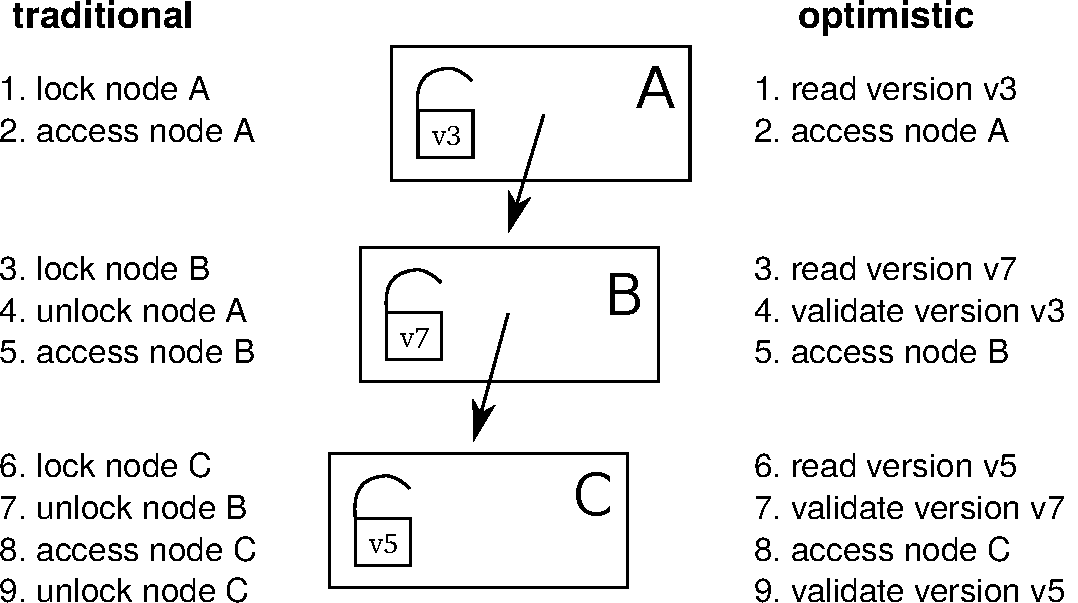
\includegraphics[width=0.65\linewidth]{olcall.pdf}
  \vspace{0.2cm}
  \caption{Comparison of a lookup operation in a 3-level tree using traditional lock coupling (left-hand side) vs.~optimistic lock coupling (right-hand side).}
  \label{fig:olc}
\end{figure}

The traditional and most common lock-based synchronization protocol for B-trees is lock coupling, which interleaves lock acquisitions while holding at most two locks at a time.
If, as we observed earlier, optimistic locks have similar semantics as traditional locks, it is natural to ask whether lock coupling can be combined with optimistic locks.
And indeed the answer is yes: One can almost mechanically translate traditional lock coupling code to optimistic lock coupling code.
This is illustrated in Figure~\ref{fig:olc}, which compares the traversal in a tree of height 3 using traditional and optimistic locks.
As the figure shows, the main difference is that locking is translated to reading the version and that unlocking becomes validation of the previously read version.
This simple change provides efficient lock-free tree traversal without the need to design a complex synchronization protocol.

It is important to emphasize the conceptual simplicity of OLC in comparison to data structures that use custom protocols like the Bw-tree~\cite{DBLP:conf/icde/LevandoskiLS13a}.
To implement lock-free access, the Bw-tree requires an indirection table, delta nodes, complex splitting and merging logic, retry logic, etc.
OLC, on the other hand, can directly be applied to B-trees mostly by adding the appropriate optimistic locking code and without modifying the node layout itself.
Therefore, OpenBw-Tree, an open source implementation of the Bw-tree, requires an order of magnitude more code than a B-tree based on OLC\footnote{Both implementations are available on GitHub: \url{https://github.com/wangziqi2016/index-microbench}}.
Given how difficult it is to develop, validate, and debug lock-free code, simplicity is obviously a major advantage.

\subsection{Correctness Aspects}

\begin{figure}
  % \centering
  %[basicstyle=\normalsize\ttfamily,showstringspaces=false,columns=fullflexible,breaklines=false,breakatwhitespace=true,numbers=none,numberstyle=\small,style=C,keepspaces=true]
\begin{lstlisting}[basicstyle=\ttfamily,language=C++,numbers=left,numberstyle=\small]
std::atomic<BTreeNode*> root;

// search for key in B+tree, returns payload in resultOut
bool lookup(Key key, Value& resultOut) {
   BTreeNode* node = root.load();
   uint64_t nodeVersion = node->readLockOrRestart();
   if (node != root.load()) // make sure the root is still the root
      restart();

   BTreeInner<Key>* parent = nullptr;
   uint64_t parentVersion = 0;

   while (node->isInner()) {
      auto inner = (BTreeInner*)node;

      // unlock parent and make current node the parent
      if (parent)
         parent->readUnlockOrRestart(parentVersion);
      parent = inner;
      parentVersion = nodeVersion;

      // search for next node
      node = inner->findChild(key);
      // validate 'inner' to ensure that 'node' pointer is valid
      inner->checkOrRestart(nodeVersion);
      // now it safe to dereference 'node' pointer (read its version)
      nodeVersion = node->readLockOrRestart();
   }

   // search in leaf and retrieve payload
   auto leaf = (BTreeLeaf*)node;
   bool success = leaf->findValue(key, resultOut);

   // unlock everything
   if (parent)
      parent->readUnlockOrRestart(parentVersion);
   node->readUnlockOrRestart(nodeVersion);

   return success;
}
\end{lstlisting}
  \vspace{0.2cm}
  \caption{B-tree lookup code using OLC. For simplicity, the restart logic is not shown.}
  \label{fig:lookup}
\end{figure}

So far, we have introduced the high-level ideas behind OLC and have stressed its similarity to traditional lock coupling.
Let us now discuss some cases where the close similarity between lock coupling and OLC breaks down.
To make this more concrete, we show the B-tree lookup code in Figure~\ref{fig:lookup}.
In the code, \texttt{readLockOrRestart} reads the lock version and \texttt{readUnlockOrRestart} validates that the read was correct.

One issue with OLC is that any pointer speculatively read from a node may point to invalid memory (if that node is modified concurrently).
Dereferencing such a pointer (e.g., to read its optimistic lock), may cause a segmentation fault or undefined behavior.
In the code shown in Figure~\ref{fig:lookup}, this problem is prevented by the extra check in line 25, which ensures that the read from the node containing the pointer was correct.
Without this additional validation, the code would in line 27 dereference the pointer speculatively read in line 23.
Note that the implementation of \texttt{checkOrRestart} is actually identical to \texttt{readUnlockOrRestart}.
We chose to give it a different name to highlight the fact that this extra check would not be necessary with read/write locks.

Another potential issue with optimistic locks is code that does not terminate.
Code that speculatively accesses a node, like an intra-node binary search, should be written in a way such that it always terminates---even in the presence of concurrent writes.
Otherwise, the validation code that detects the concurrent write will never run.
The binary search of a B-tree, for example, needs to be written in such a way that each comparison makes progress.
For some data structures that do not require loops in the traversal code (like ART) termination is trivially true.

\subsection{Implementation Details}

% implementation, efficiency
To implement an optimistic lock, one can combine the lock and the version counter into a single 64-bit\footnote{Even after subtracting one bit for the lock status, a back-of-the-envelope calculation can show that 63 bits are large enough to never overflow in practice.} word~\cite{artsync}.
A typical read operation will therefore merely consist of reading this version counter atomically.
In C++11 this can be implemented using the \texttt{std::atomic} type.

On x86, atomic reads are cheap because of x86's strong memory order guarantees.
No memory fences are required for sequentially-consistent loads, which are translated (by both GCC and clang) into standard \texttt{MOV} instructions.
Hence, the only effect of \texttt{std::atomic} for loads is preventing instruction re-ordering.
This makes version access and validation cheap.
Acquiring and releasing an optimistic lock in exclusive mode has comparable cost to a traditional lock:
A fairly expensive sequentially-consistent store is needed for acquiring a lock, while a standard \texttt{MOV} suffices for releasing it.
A simple sinlock-based implementation of optimistic locks can be found in the appendix of an earlier paper~\cite{artsync}.

OLC code must be able to handle restarts since validation or lock upgrade can fail due to concurrent writers.
Restarts can easily be implemented by wrapping the data structure operation in a loop (for simplicity not shown in Figure~\ref{fig:lookup}).
Such a loop also enables limiting the number of optimistic retry operations and falling back to pessimistic locking in cases of very heavy contention.
The ability to fall back to traditional locking is a major advantage of OLC in terms of robustness over lock-free approaches, which do not have this option.

In addition to the optimistic shared mode and the exclusive mode, optimistic locks also support a ``shared pessimistic'' mode, which physically acquires the lock in shared mode (allowing multiple concurrent readers but no writers).
This mode is useful for table (or range) scans that touch many tuples on a leaf page (which would otherwise easily abort).
Finally, let us mention that large range scans and table scans, should be broken up into several per-node traversals as is done in the LeanStore~\cite{leanstore} system.

Like all lock-free data structures, but unlike traditional locking and Hardware Transactional Memory~\cite{DBLP:conf/hpca/KarnagelDRLLSL14,DBLP:journals/pvldb/MakreshanskiLS15,htmtkde}, OLC requires care when deleting (and reusing) nodes.
The reason is that a deleting thread can never be sure that a node can be reclaimed because other threads might still be optimistically reading from that node.
Therefore, standard solutions like epoch-based reclamation~\cite{DBLP:conf/sosp/TuZKLM13}, hazard pointers~\cite{DBLP:journals/tpds/Michael04}, or optimized hazard pointers~\cite{DBLP:conf/spaa/BalmauGHZ16} need to be used.
These memory reclamation techniques are, however, largely orthogonal to the synchronization protocol itself.

%-lock-free is not a strong guarantee

\newpage
\section{Evaluation}\label{sec:evaluation}

Let us now experimentally evaluate the overhead and scalability of OLC.
For the experiments, we use an in-memory B+tree implemented in C++11 using templates, which is configured to use nodes of 4096 bytes, random 8 byte keys, and 8 byte payloads.
Based on this B-tree, we compare the following synchronization approaches:
\begin{itemize}
\item an OLC implementation\footnote{An almost identical OLC implementation is available on github: \url{https://github.com/wangziqi2016/index-microbench/tree/master/BTreeOLC}}
\item a variant based on traditional lock coupling and read/write locks
\item the unsynchronized B-tree, which obviously is only correct for read-only workloads but allows measuring the overhead of synchronization
\end{itemize}
Note that earlier work has compared the OLC implementation with a Bw-tree implementation~\cite{buzzword} and other state-of-the-art in-memory index structures.

We use a Haswell EP system with an Intel Xeon E5-2687W v3 CPU, which has 10 cores (20 ``Hyper-Threads'') and 25~MB of L3 cache.
The system is running Ubuntu 18.10 and we use GCC 8.2.0 to compile our code.
The CPU counters are obtained using the Linux perf API\footnote{We use the following convenience wrapper: \url{https://github.com/viktorleis/perfevent}}.

\begin{table}
  \caption{Performance and CPU counters for lookup and insert operations in a B-tree with 100M keys. We perform 100M operations and normalize the CPU counters by that number.}
  \label{tab:overhead}
  \centering
  \begin{tabular}{lrrrrrrr}\toprule
                    &         &        &        & instruc-  & L1     & L3     & branch \\
                    & threads & M op/s & cycles & tions & misses & misses & misses \\\midrule
lookup (no sync.)   & 1       & 1.72   & 2028   & 283     & 39.1   & 14.9   & 16.1   \\
lookup (OLC)        & 1       & 1.65   & 2107   & 370     & 43.9   & 15.1   & 16.7   \\
lookup (lock coup.) & 1       & 1.72   & 2078   & 365     & 42.3   & 16.9   & 15.7   \\\midrule
insert (no sync.)   & 1       & 1.51   & 2286   & 530     & 59.8   & 31.1   & 17.3   \\
insert (OLC)        & 1       & 1.50   & 2303   & 629     & 61.2   & 31.1   & 16.5   \\
insert (lock coup.) & 1       & 1.41   & 2473   & 644     & 61.0   & 31.0   & 17.2   \\\midrule
lookup (no sync.)   & 10      & 15.48  & 2058   & 283     & 38.6   & 15.5   & 16.0   \\
lookup (OLC)        & 10      & 14.60  & 2187   & 370     & 43.8   & 15.8   & 16.8   \\
lookup (lock coup.) & 10      & 5.71   & 5591   & 379     & 54.2   & 17.0   & 14.8   \\\midrule
insert (no sync.)   & 10      & -      & -      & -       & -      & -      & -      \\
insert (OLC)        & 10      & 10.46  & 2940   & 656     & 62.0   & 32.5   & 16.8   \\
insert (lock coup.) & 10      & 7.55   & 4161   & 667     & 75.0   & 28.6   & 16.2   \\
    \bottomrule
\end{tabular}
\end{table}

Table~\ref{tab:overhead} compares the performance and CPU counters for lookup and insert operations in a B-tree with 100M keys.
With {\em single-threaded} execution, we observe that all three approaches have very similar performance.
Adding traditional or optimistic locks to unsynchronized B-tree code results in up to 30\% of additional instructions without affecting single-threaded performance much.

\begin{figure}
  \centering
  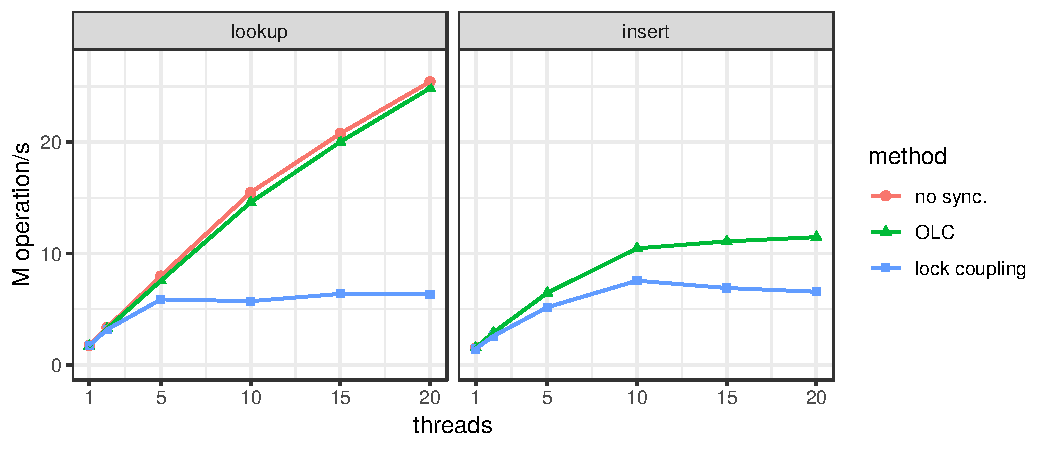
\includegraphics[width=\linewidth]{scale.pdf}
  \vspace{0.2cm}
  \caption{Scalability on 10-core system for B-tree operations (100M values).}
  \label{fig:scale}
\end{figure}

As Figure~\ref{fig:scale} shows, the results change dramatically once we use multiple threads.
For lookup, the scalability of OLC is near-linear up to 20 threads, even though the system has only 10 ``real cores''.
The OLC scalability for insert is also respectable (though not quite as linear because multi-threaded insertion approaches the memory bandwidth of our processor).
The figure also shows that the results of traditional lock coupling with read/write locks are significantly worse than OLC.
With 20 threads, lookup with OLC is 3.9$\times$ faster than traditional lock coupling.

\section{Summary}\label{sec:conc}

Optimistic Lock Coupling (OLC) is an effective synchronization method that combines the simplicity of traditional lock coupling with the superior scalability of lock-free approaches.
OLC is widely applicable and has already been successfully used to synchronize several data structures, including B-trees, binary search trees, and different trie variants.
These features make it highly attractive for modern database systems as well as performance-critical systems software in general.

\begin{thebibliography}{10}

\bibitem{DBLP:conf/spaa/BalmauGHZ16}
O.~Balmau, R.~Guerraoui, M.~Herlihy, and I.~Zablotchi.
\newblock Fast and robust memory reclamation for concurrent data structures.
\newblock In {\em SPAA}, 2016.

\bibitem{DBLP:journals/acta/BayerS77}
R.~Bayer and M.~Schkolnick.
\newblock Concurrency of operations on {B}-trees.
\newblock {\em Acta Informatica}, 9, 1977.

\bibitem{hot}
R.~Binna, E.~Zangerle, M.~Pichl, G.~Specht, and V.~Leis.
\newblock {HOT}: A height optimized trie index for main-memory database
  systems.
\newblock In {\em SIGMOD}, 2018.

\bibitem{DBLP:conf/ppopp/BronsonCCO10}
N.~G. Bronson, J.~Casper, H.~Chafi, and K.~Olukotun.
\newblock A practical concurrent binary search tree.
\newblock In {\em PPOPP}, 2010.

\bibitem{DBLP:conf/vldb/ChaHKK01}
S.~K. Cha, S.~Hwang, K.~Kim, and K.~Kwon.
\newblock Cache-conscious concurrency control of main-memory indexes on
  shared-memory multiprocessor systems.
\newblock In {\em VLDB}, 2001.

\bibitem{intel}
I.~Cutress.
\newblock {Intel} goes for 48-cores: {Cascade-AP} with multi-chip package
  coming soon.
\newblock
  \url{https://www.anandtech.com/show/13535/intel-goes-for-48cores-cascade-ap},
  2018 (accessed January, 2019).

\bibitem{DBLP:conf/cidr/FaleiroA17}
J.~M. Faleiro and D.~J. Abadi.
\newblock Latch-free synchronization in database systems: Silver bullet or
  fool's gold?
\newblock In {\em CIDR}, 2017.

\bibitem{DBLP:journals/ftdb/Graefe11}
G.~Graefe.
\newblock Modern {B}-tree techniques.
\newblock {\em Foundations and Trends in Databases}, 3(4), 2011.

\bibitem{DBLP:conf/hpca/KarnagelDRLLSL14}
T.~Karnagel, R.~Dementiev, R.~Rajwar, K.~Lai, T.~Legler, B.~Schlegel, and
  W.~Lehner.
\newblock Improving in-memory database index performance with
  {Intel}\({}^{\mbox{{\textregistered}}}\) transactional synchronization
  extensions.
\newblock In {\em HPCA}, 2014.

\bibitem{DBLP:journals/tods/LehmanY81}
P.~L. Lehman and S.~B. Yao.
\newblock Efficient locking for concurrent operations on {B}-trees.
\newblock {\em {ACM} Trans. Database Syst.}, 6(4), 1981.

\bibitem{leanstore}
V.~Leis, M.~Haubenschild, A.~Kemper, and T.~Neumann.
\newblock Leanstore: In-memory data management beyond main memory.
\newblock In {\em ICDE}, 2018.

\bibitem{art}
V.~Leis, A.~Kemper, and T.~Neumann.
\newblock The adaptive radix tree: {ARTful} indexing for main-memory databases.
\newblock In {\em ICDE}, 2013.

\bibitem{htmtkde}
V.~Leis, A.~Kemper, and T.~Neumann.
\newblock Scaling {HTM}-supported database transactions to many cores.
\newblock {\em {IEEE} Trans. Knowl. Data Eng.}, 28(2), 2016.

\bibitem{artsync}
V.~Leis, F.~Scheibner, A.~Kemper, and T.~Neumann.
\newblock The {ART} of practical synchronization.
\newblock In {\em DaMoN}, 2016.

\bibitem{DBLP:conf/icde/LevandoskiLS13a}
J.~J. Levandoski, D.~B. Lomet, and S.~Sengupta.
\newblock The {Bw}-tree: A {B}-tree for new hardware platforms.
\newblock In {\em ICDE}, 2013.

\bibitem{DBLP:journals/pvldb/MakreshanskiLS15}
D.~Makreshanski, J.~J. Levandoski, and R.~Stutsman.
\newblock To lock, swap, or elide: On the interplay of hardware transactional
  memory and lock-free indexing.
\newblock {\em {PVLDB}}, 8(11), 2015.

\bibitem{DBLP:dblp_conf/eurosys/MaoKM12}
Y.~Mao, E.~Kohler, and R.~T. Morris.
\newblock Cache craftiness for fast multicore key-value storage.
\newblock In {\em EuroSys}, 2012.

\bibitem{DBLP:journals/tpds/Michael04}
M.~M. Michael.
\newblock Hazard pointers: Safe memory reclamation for lock-free objects.
\newblock {\em {IEEE} Trans. Parallel Distrib. Syst.}, 15(6), 2004.

\bibitem{DBLP:journals/jacm/ShalevS06}
O.~Shalev and N.~Shavit.
\newblock Split-ordered lists: Lock-free extensible hash tables.
\newblock {\em J. {ACM}}, 53(3), 2006.

\bibitem{amd}
A.~Shilov.
\newblock {AMD} previews {EPYC} ‘{Rome}’ processor: Up to 64 {Zen} 2 cores.
\newblock
  \url{https://www.anandtech.com/show/13561/amd-previews-epyc-rome-processor-up-to-64-zen-2-cores},
  2018 (accessed January, 2019).

\bibitem{DBLP:conf/sosp/TuZKLM13}
S.~Tu, W.~Zheng, E.~Kohler, B.~Liskov, and S.~Madden.
\newblock Speedy transactions in multicore in-memory databases.
\newblock In {\em SOSP}, 2013.

\bibitem{buzzword}
Z.~Wang, A.~Pavlo, H.~Lim, V.~Leis, H.~Zhang, M.~Kaminsky, and D.~Andersen.
\newblock Building a {Bw}-tree takes more than just buzz words.
\newblock In {\em SIGMOD}, 2018.

\end{thebibliography}


%\bibliographystyle{abbrv}
%\bibliography{main}

\end{document}

\end{article}

\begin{article}
{Symphony: Towards Trustworthy Question Answering and Verification using RAG over Multimodal Data Lakes}
{Nan Tang, Chenyu Yang, Zhengxuan Zhang, Yuyu Luo, Ju Fan, Lei Cao, Sam Madden, Alon Halevy}
\setcounter{section}{0}
\pdfminorversion=5
\documentclass[11pt]{article}
\usepackage{deauthor,times,graphicx,caption,microtype}
\usepackage{hyperref}
\usepackage{listings}
\usepackage{booktabs}

\begin{document}

\title{Optimistic Lock Coupling: A Scalable and Efficient General-Purpose Synchronization Method}

\author{Viktor Leis, Michael Haubenschild\raisebox{0.9ex}{$\ast$}, Thomas Neumann\\ Technische Universit{\"a}t M{\"u}nchen \hspace{0.7cm} Tableau Software\raisebox{0.9ex}{$\ast$} \\ {\{leis,neumann\}{@}in.tum.de} \hspace{0.7cm} {mhaubenschild{@}tableau.com\raisebox{0.9ex}{$\ast$}}}

\maketitle

\begin{abstract}
As the number of cores on commodity processors continues to increase, scalability becomes more and more crucial for overall performance.
Scalable and efficient concurrent data structures are particularly important, as these are often the building blocks of parallel algorithms.
Unfortunately, traditional synchronization techniques based on fine-grained locking have been shown to be unscalable on modern multi-core CPUs.
Lock-free data structures, on the other hand, are extremely difficult to design and often incur significant overhead.

In this work, we make the case for Optimistic Lock Coupling as a practical alternative to both traditional locking and the lock-free approach.
We show that Optimistic Lock Coupling is highly scalable and almost as simple to implement as traditional lock coupling.
Another important advantage is that it is easily applicable to most tree-like data structures.
We therefore argue that Optimistic Lock Coupling, rather than a complex and error-prone custom synchronization protocol, should be the default choice for performance-critical data structures.
\end{abstract}

\section{Introduction}

% more and more cores
Today, Intel's commodity server processors have up to 28 cores and its upcoming microarchitecture will have up to 48 cores per socket~\cite{intel}.
Similarly, AMD currently stands at 32 cores and this number is expected to double in the next generation~\cite{amd}.
Since both platforms support simultaneous multithreading (also known as hyperthreading), affordable commodity servers (with up to two sockets) will soon routinely have between 100 and 200 hardware threads.

% data structure scalability is important
With such a high degree of hardware parallelism, efficient data processing crucially depends on how well concurrent data structures scale.
Internally, database systems use a plethora of data structures like table heaps, internal work queues, and, most importantly, index structures.
Any of these can easily become a scalability (and therefore overall performance) bottleneck on many-core CPUs.

% traditional synchronization: fine-grained locks, slow, cache invalidation
Traditionally, database systems synchronize internal data structures using fine-grained reader/writer locks\footnote{In this work, we focus on data structure synchronization rather than high-level transaction semantics and therefore use the term {\em lock} for what would typically be called {\em latch} in the database literature. We thus follow common computer science (rather than database) terminology.}.
Unfortunately, while fine-grained locking makes lock contention unlikely, it still results in bad scalability because lock acquisition and release require writing to shared memory.
Due to the way cache coherency is implemented on modern multi-core CPUs, these writes cause additional cache misses\footnote{The cache coherency protocol ensures that all copies of a cache line on other cores are invalidated before the write can proceed.} and the cache line containing the lock's internal data becomes a point of physical contention.
As a result, any frequently-accessed lock (e.g., the lock of the root node of a B-tree) severely limits scalability.

% lock-free bw-tree: no more latches, but indirections, extremely complex
Lock-free data structures like the Bw-tree~\cite{DBLP:conf/icde/LevandoskiLS13a} (a lock-free B-tree variant) or the Split-Ordered List~\cite{DBLP:journals/jacm/ShalevS06} (a lock-free hash table) do not acquire any locks and therefore generally scale much better than locking-based approaches (in particular for read-mostly workloads).
However, lock-free synchronization has other downsides:
First, it is very difficult and results in extremely complex and error-prone code (when compared to locking).
Second, because the functionality of atomic primitives provided by the hardware (e.g., atomically compare-and-swap 8 bytes) is limited, complex operations require additional indirections within the data structure.
For example, the Bw-tree requires an indirection table and the Split-Ordered List requires ``dummy nodes'', resulting in overhead due to additional cache misses.

% OLC for the win
In this paper we make the case for {\em Optimistic Lock Coupling (OLC)}, a synchronization method that combines some of the best properties of lock-based and lock-free synchronization.
OLC utilizes a special lock type that can be used in two modes:
The first mode is similar to a traditional mutex and excludes other threads by physically acquiring the underlying lock.
In the second mode, reads can proceed optimistically by validating a version counter that is embedded in the lock (similar to optimistic concurrency control).
The first mode is typically used by writers and the second mode by readers.
Besides this special lock type, OLC is based on the observation that optimistic lock validations can be interleaved/coupled---similar to the pair-wise interleaved lock acquisition of traditional lock coupling.
Hence, the name Optimistic Lock Coupling.

OLC has a number of desirable features:
\begin{itemize}
\item By reducing the number of writes to shared memory locations and thereby avoiding cache invalidations, it {\bf scales well} for most workloads.
\item In comparison to unsynchronized code, it requires few additional CPU instructions making it {\bf efficient}.
\item OLC is {\bf widely applicable} to different data structures. It has already been successfully used for synchronizing binary search trees~\cite{DBLP:conf/ppopp/BronsonCCO10}, tries~\cite{artsync}, trie/B-tree hybrids~\cite{DBLP:dblp_conf/eurosys/MaoKM12}, and B-trees~\cite{buzzword}.
\item In comparison to the lock-free paradigm, it is also {\bf easy to use} and requires few modifications to existing, single-threaded data structures.
\end{itemize}
Despite these positive features and its simplicity, OLC is not yet widely known.
The goal of this paper is therefore to popularize this simple idea and to make a case for it.
We argue that OLC deserves to be widely known.
It is a good default synchronization paradigm---more complex, data structure-specific protocols are seldom beneficial.

The rest of the paper is organized as follows.
Section~\ref{sec:related} discusses related work, tracing the history of OLC and its underlying ideas in the literature.
The core of the paper is Section~\ref{sec:olc}, which describes the ideas behind OLC and how it can be used to synchronize complex data structures.
In Section~\ref{sec:evaluation} we experimentally show that OLC has low overhead and scales well when used to synchronize an in-memory B-tree.
We summarize the paper in Section~\ref{sec:conc}.

\newpage
\section{Related Work}\label{sec:related}

Lock coupling has been proposed as a method for allowing concurrent operations on B-trees in 1977~\cite{DBLP:journals/acta/BayerS77}.
This traditional and still widely-used method, described in detail in Graefe's B-tree survey~\cite{DBLP:journals/ftdb/Graefe11}, is also called ``latch coupling'', ``hand-over-hand locking'', and ``crabbing''.
Because at most two locks are held at-a-time during tree traversal, this technique seemingly allows for a high degree of parallelism---in particular if read/write locks are used to enable inner nodes to be locked in shared mode.
However, as we show in Section~\ref{sec:evaluation}, on modern hardware lock acquisition (even in shared mode) results in suboptimal scalability.

An early alternative from 1981 is a B-tree variant called B-link tree~\cite{DBLP:journals/tods/LehmanY81}, which only holds a single lock at a time.
It is based on the observation that between the release of the parent lock and the acquisition of the child lock, the only ``dangerous'' thing that could have happened is the split of a child node (assuming one does not implement merge operations).
Thus, when a split happens, the key being searched might end up on a neighboring node to the right of the current child node.
A B-link tree traversal therefore detects this condition and, if needed, transparently proceeds to the neighboring node.
Releasing the parent lock early is highly beneficial when the child node needs to be fetched from disk.
For in-memory workloads, however, the B-link tree has the same scalability issues as lock coupling (it acquires just as many locks).

The next major advance, Optimistic Latch-Free Index Traversal (OLFIT)~\cite{DBLP:conf/vldb/ChaHKK01}, was proposed in 2001.
OLFIT introduced the idea of a combined lock/update counter, which we call {\em optimistic lock}. % , for lack of a better name,
Based on these per-node optimistic locks and the synchronization protocol of the B-link tree, OLFIT finally achieves good scalability on parallel processors.
The OLFIT protocol is fairly complex, as it requires both the non-trivial B-link protocol and optimistic locks.
Furthermore, like the B-link tree protocol, it does not support merging nodes, and is specific to B-trees (cannot easily be applied to other data structures).

In the following two decades, the growth of main-memory capacity led to much research into other data structures besides the venerable B-tree.
Particularly relevant for our discussion is Bronson et al.'s~\cite{DBLP:conf/ppopp/BronsonCCO10} concurrent binary search tree, which is based on optimistic version validation and has a sophisticated, data structure-specific synchronization protocol.
To the best of our knowledge, this 2010 paper is the first that, as part of its protocol, interleaves version validation across nodes---rather than validating each node separately like OLFIT.
In that paper, this idea is called ``hand-over-hand, optimistic validation'', while we prefer the term Optimistic Lock Coupling to highlight the close resemblance to traditional lock coupling.
Similarly, Mao et al.'s~\cite{DBLP:dblp_conf/eurosys/MaoKM12} Masstree (a concurrent hybrid trie/B-tree) is also based on the same ideas, but again uses them as part of a more complex protocol.

The Adaptive Radix Tree (ART)~\cite{art} is another recent in-memory data structure, which we proposed in 2013.
In contrast to the two data structures just mentioned, it was originally designed with single-threaded performance in mind without supporting concurrency.
To add support for concurrency, we initially started designing a custom protocol called Read-Optimized Write Exclusion (ROWEX)~\cite{artsync}, which turned out to be non-trivial and requires modifications of the underlying data structure\footnote{Note that ROWEX is already easier to apply to existing data structures than the lock-free approach. The difficulty depends on the data structure. Applying ROWEX is hard for B-trees with sorted keys and fairly easy for copy-on-write data structures like the Height Optimized Trie~\cite{hot}---with ART being somewhere in the middle.}.
However, fairly late in the project, we also realized, that OLC {\em alone} (rather than as part of a more complex protocol) is sufficient to synchronize ART.
No other changes to the data structure were necessary.
Both approaches were published and experimentally evaluated in a followup paper~\cite{artsync}, which shows that, despite its simplicity, OLC is efficient, scalable, and generally outperforms ROWEX.

Similar results were recently published regarding B-trees~\cite{buzzword}.
In this experimental study a simple OLC-based synchronization outperformed the Bw-tree~\cite{DBLP:conf/icde/LevandoskiLS13a}, a complex lock-free synchronization approach.
Another recent paper shows that for write-intensive workloads, locking often performs better than lock-free synchronization~\cite{DBLP:conf/cidr/FaleiroA17}.
These experiences indicate that OLC is a general-purpose synchronization paradigm and motivate the current paper.

%foster b-tree\cite{DBLP:journals/tods/GraefeKK12}
%Shasha theory~\cite{DBLP:journals/tods/ShashaG88}

\section{Optimistic Lock Coupling}\label{sec:olc}

% locks suck
The standard technique for inter-thread synchronization is mutual exclusion using fine-grained locks.
In a B-tree, for example, every node usually has its own associated lock, which is acquired before accessing that node.
The problem of locking on modern multi- and many-core processors is that lock acquisition and release require writing to the shared memory location that implements the lock.
This write causes exclusive ownership of the underlying cache line and invalidates copies of it on all other processor cores.
For hierarchical, tree-like data structures, the lock of the root node becomes a point of physical contention---even in read-only workloads and even when read/write locks are used.
Depending on the specific data structure, number of cores, cache coherency protocol implementation, cache topology, whether Non-Uniform Memory Access (NUMA) is used, locking can even result in multi-threaded performance that is worse than single-threaded execution.

% in b-trees this happens very much
The inherent pessimism of locking is particularly unfortunate for B-trees:
Despite the fact that logical modifications of the root node are very infrequent, every B-tree operation must lock the root node during tree traversal\footnote{To a lesser extent this obviously applies to all inner nodes, not just the root.}.
Even the vast majority of update operations (with the exception of splits and merges), only modify a single leaf node.
These observations indicate that a more optimistic approach, which does not require locking inner nodes, would be very beneficial for B-trees.

\subsection{Optimistic Locks}

% optimism to the rescue
As the name indicates, optimistic locks try to solve the scalability issues of traditional locks using an optimistic approach.
Instead of always physically acquiring locks, even for nodes that are unlikely to be modified simultaneously, after-the-fact validation is used to detect conflicts.
This is done by augmenting each lock with a version/update counter that is incremented on every modification.
Using this version counter, readers can optimistically proceed before validating that the version did not change to ensure that the read was safe.
If validation fails, the operation is restarted.

% details on opt locks
Using optimistic locks, a read-only node access (i.e., the majority of all operations in a B-tree) does not acquire the lock and does not increment the version counter.
Instead, it performs the following steps:
\begin{enumerate}
\item read lock version (restart if lock is not free)
\item access node
\item read the version again and validate that it has not changed in the meantime
\end{enumerate}
If the last step (the validation) fails, the operation has to be restarted.
Write operations, on the other hand, are more similar to traditional locking:
\begin{enumerate}
\item acquire lock (wait if necessary)
\item access/write to node
\item increment version and unlock node
\end{enumerate}
Writes can therefore protect a node from other writes.

% similar to locks
As we observed in an earlier paper~\cite{artsync}, because of similar semantics, optimistic locks can be hidden behind an API very similar to traditional read/write locks.
Both approaches have an exclusive lock mode, and acquiring a traditional lock in shared mode is analogous to optimistic version validation.
Furthermore, like with some implementations of traditional read/write locks, optimistic locks allow upgrading a shared lock to an exclusive lock.
Lock upgrades are, for example, used to avoid most B-tree update operations from having to lock inner nodes.
In our experience, the close resemblance of optimistic and traditional locks simplifies the reasoning about optimistic locks;
one can apply similar thinking as in traditional lock-based protocols.

\subsection{Lock Coupling with Optimistic Locks}

\begin{figure}
  \centering
  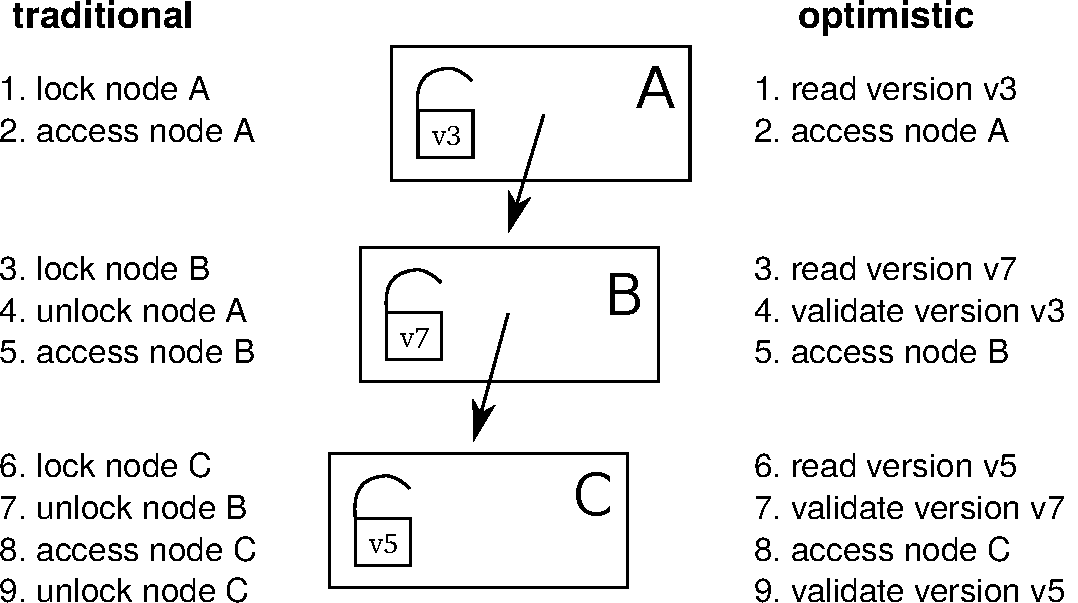
\includegraphics[width=0.65\linewidth]{olcall.pdf}
  \vspace{0.2cm}
  \caption{Comparison of a lookup operation in a 3-level tree using traditional lock coupling (left-hand side) vs.~optimistic lock coupling (right-hand side).}
  \label{fig:olc}
\end{figure}

The traditional and most common lock-based synchronization protocol for B-trees is lock coupling, which interleaves lock acquisitions while holding at most two locks at a time.
If, as we observed earlier, optimistic locks have similar semantics as traditional locks, it is natural to ask whether lock coupling can be combined with optimistic locks.
And indeed the answer is yes: One can almost mechanically translate traditional lock coupling code to optimistic lock coupling code.
This is illustrated in Figure~\ref{fig:olc}, which compares the traversal in a tree of height 3 using traditional and optimistic locks.
As the figure shows, the main difference is that locking is translated to reading the version and that unlocking becomes validation of the previously read version.
This simple change provides efficient lock-free tree traversal without the need to design a complex synchronization protocol.

It is important to emphasize the conceptual simplicity of OLC in comparison to data structures that use custom protocols like the Bw-tree~\cite{DBLP:conf/icde/LevandoskiLS13a}.
To implement lock-free access, the Bw-tree requires an indirection table, delta nodes, complex splitting and merging logic, retry logic, etc.
OLC, on the other hand, can directly be applied to B-trees mostly by adding the appropriate optimistic locking code and without modifying the node layout itself.
Therefore, OpenBw-Tree, an open source implementation of the Bw-tree, requires an order of magnitude more code than a B-tree based on OLC\footnote{Both implementations are available on GitHub: \url{https://github.com/wangziqi2016/index-microbench}}.
Given how difficult it is to develop, validate, and debug lock-free code, simplicity is obviously a major advantage.

\subsection{Correctness Aspects}

\begin{figure}
  % \centering
  %[basicstyle=\normalsize\ttfamily,showstringspaces=false,columns=fullflexible,breaklines=false,breakatwhitespace=true,numbers=none,numberstyle=\small,style=C,keepspaces=true]
\begin{lstlisting}[basicstyle=\ttfamily,language=C++,numbers=left,numberstyle=\small]
std::atomic<BTreeNode*> root;

// search for key in B+tree, returns payload in resultOut
bool lookup(Key key, Value& resultOut) {
   BTreeNode* node = root.load();
   uint64_t nodeVersion = node->readLockOrRestart();
   if (node != root.load()) // make sure the root is still the root
      restart();

   BTreeInner<Key>* parent = nullptr;
   uint64_t parentVersion = 0;

   while (node->isInner()) {
      auto inner = (BTreeInner*)node;

      // unlock parent and make current node the parent
      if (parent)
         parent->readUnlockOrRestart(parentVersion);
      parent = inner;
      parentVersion = nodeVersion;

      // search for next node
      node = inner->findChild(key);
      // validate 'inner' to ensure that 'node' pointer is valid
      inner->checkOrRestart(nodeVersion);
      // now it safe to dereference 'node' pointer (read its version)
      nodeVersion = node->readLockOrRestart();
   }

   // search in leaf and retrieve payload
   auto leaf = (BTreeLeaf*)node;
   bool success = leaf->findValue(key, resultOut);

   // unlock everything
   if (parent)
      parent->readUnlockOrRestart(parentVersion);
   node->readUnlockOrRestart(nodeVersion);

   return success;
}
\end{lstlisting}
  \vspace{0.2cm}
  \caption{B-tree lookup code using OLC. For simplicity, the restart logic is not shown.}
  \label{fig:lookup}
\end{figure}

So far, we have introduced the high-level ideas behind OLC and have stressed its similarity to traditional lock coupling.
Let us now discuss some cases where the close similarity between lock coupling and OLC breaks down.
To make this more concrete, we show the B-tree lookup code in Figure~\ref{fig:lookup}.
In the code, \texttt{readLockOrRestart} reads the lock version and \texttt{readUnlockOrRestart} validates that the read was correct.

One issue with OLC is that any pointer speculatively read from a node may point to invalid memory (if that node is modified concurrently).
Dereferencing such a pointer (e.g., to read its optimistic lock), may cause a segmentation fault or undefined behavior.
In the code shown in Figure~\ref{fig:lookup}, this problem is prevented by the extra check in line 25, which ensures that the read from the node containing the pointer was correct.
Without this additional validation, the code would in line 27 dereference the pointer speculatively read in line 23.
Note that the implementation of \texttt{checkOrRestart} is actually identical to \texttt{readUnlockOrRestart}.
We chose to give it a different name to highlight the fact that this extra check would not be necessary with read/write locks.

Another potential issue with optimistic locks is code that does not terminate.
Code that speculatively accesses a node, like an intra-node binary search, should be written in a way such that it always terminates---even in the presence of concurrent writes.
Otherwise, the validation code that detects the concurrent write will never run.
The binary search of a B-tree, for example, needs to be written in such a way that each comparison makes progress.
For some data structures that do not require loops in the traversal code (like ART) termination is trivially true.

\subsection{Implementation Details}

% implementation, efficiency
To implement an optimistic lock, one can combine the lock and the version counter into a single 64-bit\footnote{Even after subtracting one bit for the lock status, a back-of-the-envelope calculation can show that 63 bits are large enough to never overflow in practice.} word~\cite{artsync}.
A typical read operation will therefore merely consist of reading this version counter atomically.
In C++11 this can be implemented using the \texttt{std::atomic} type.

On x86, atomic reads are cheap because of x86's strong memory order guarantees.
No memory fences are required for sequentially-consistent loads, which are translated (by both GCC and clang) into standard \texttt{MOV} instructions.
Hence, the only effect of \texttt{std::atomic} for loads is preventing instruction re-ordering.
This makes version access and validation cheap.
Acquiring and releasing an optimistic lock in exclusive mode has comparable cost to a traditional lock:
A fairly expensive sequentially-consistent store is needed for acquiring a lock, while a standard \texttt{MOV} suffices for releasing it.
A simple sinlock-based implementation of optimistic locks can be found in the appendix of an earlier paper~\cite{artsync}.

OLC code must be able to handle restarts since validation or lock upgrade can fail due to concurrent writers.
Restarts can easily be implemented by wrapping the data structure operation in a loop (for simplicity not shown in Figure~\ref{fig:lookup}).
Such a loop also enables limiting the number of optimistic retry operations and falling back to pessimistic locking in cases of very heavy contention.
The ability to fall back to traditional locking is a major advantage of OLC in terms of robustness over lock-free approaches, which do not have this option.

In addition to the optimistic shared mode and the exclusive mode, optimistic locks also support a ``shared pessimistic'' mode, which physically acquires the lock in shared mode (allowing multiple concurrent readers but no writers).
This mode is useful for table (or range) scans that touch many tuples on a leaf page (which would otherwise easily abort).
Finally, let us mention that large range scans and table scans, should be broken up into several per-node traversals as is done in the LeanStore~\cite{leanstore} system.

Like all lock-free data structures, but unlike traditional locking and Hardware Transactional Memory~\cite{DBLP:conf/hpca/KarnagelDRLLSL14,DBLP:journals/pvldb/MakreshanskiLS15,htmtkde}, OLC requires care when deleting (and reusing) nodes.
The reason is that a deleting thread can never be sure that a node can be reclaimed because other threads might still be optimistically reading from that node.
Therefore, standard solutions like epoch-based reclamation~\cite{DBLP:conf/sosp/TuZKLM13}, hazard pointers~\cite{DBLP:journals/tpds/Michael04}, or optimized hazard pointers~\cite{DBLP:conf/spaa/BalmauGHZ16} need to be used.
These memory reclamation techniques are, however, largely orthogonal to the synchronization protocol itself.

%-lock-free is not a strong guarantee

\newpage
\section{Evaluation}\label{sec:evaluation}

Let us now experimentally evaluate the overhead and scalability of OLC.
For the experiments, we use an in-memory B+tree implemented in C++11 using templates, which is configured to use nodes of 4096 bytes, random 8 byte keys, and 8 byte payloads.
Based on this B-tree, we compare the following synchronization approaches:
\begin{itemize}
\item an OLC implementation\footnote{An almost identical OLC implementation is available on github: \url{https://github.com/wangziqi2016/index-microbench/tree/master/BTreeOLC}}
\item a variant based on traditional lock coupling and read/write locks
\item the unsynchronized B-tree, which obviously is only correct for read-only workloads but allows measuring the overhead of synchronization
\end{itemize}
Note that earlier work has compared the OLC implementation with a Bw-tree implementation~\cite{buzzword} and other state-of-the-art in-memory index structures.

We use a Haswell EP system with an Intel Xeon E5-2687W v3 CPU, which has 10 cores (20 ``Hyper-Threads'') and 25~MB of L3 cache.
The system is running Ubuntu 18.10 and we use GCC 8.2.0 to compile our code.
The CPU counters are obtained using the Linux perf API\footnote{We use the following convenience wrapper: \url{https://github.com/viktorleis/perfevent}}.

\begin{table}
  \caption{Performance and CPU counters for lookup and insert operations in a B-tree with 100M keys. We perform 100M operations and normalize the CPU counters by that number.}
  \label{tab:overhead}
  \centering
  \begin{tabular}{lrrrrrrr}\toprule
                    &         &        &        & instruc-  & L1     & L3     & branch \\
                    & threads & M op/s & cycles & tions & misses & misses & misses \\\midrule
lookup (no sync.)   & 1       & 1.72   & 2028   & 283     & 39.1   & 14.9   & 16.1   \\
lookup (OLC)        & 1       & 1.65   & 2107   & 370     & 43.9   & 15.1   & 16.7   \\
lookup (lock coup.) & 1       & 1.72   & 2078   & 365     & 42.3   & 16.9   & 15.7   \\\midrule
insert (no sync.)   & 1       & 1.51   & 2286   & 530     & 59.8   & 31.1   & 17.3   \\
insert (OLC)        & 1       & 1.50   & 2303   & 629     & 61.2   & 31.1   & 16.5   \\
insert (lock coup.) & 1       & 1.41   & 2473   & 644     & 61.0   & 31.0   & 17.2   \\\midrule
lookup (no sync.)   & 10      & 15.48  & 2058   & 283     & 38.6   & 15.5   & 16.0   \\
lookup (OLC)        & 10      & 14.60  & 2187   & 370     & 43.8   & 15.8   & 16.8   \\
lookup (lock coup.) & 10      & 5.71   & 5591   & 379     & 54.2   & 17.0   & 14.8   \\\midrule
insert (no sync.)   & 10      & -      & -      & -       & -      & -      & -      \\
insert (OLC)        & 10      & 10.46  & 2940   & 656     & 62.0   & 32.5   & 16.8   \\
insert (lock coup.) & 10      & 7.55   & 4161   & 667     & 75.0   & 28.6   & 16.2   \\
    \bottomrule
\end{tabular}
\end{table}

Table~\ref{tab:overhead} compares the performance and CPU counters for lookup and insert operations in a B-tree with 100M keys.
With {\em single-threaded} execution, we observe that all three approaches have very similar performance.
Adding traditional or optimistic locks to unsynchronized B-tree code results in up to 30\% of additional instructions without affecting single-threaded performance much.

\begin{figure}
  \centering
  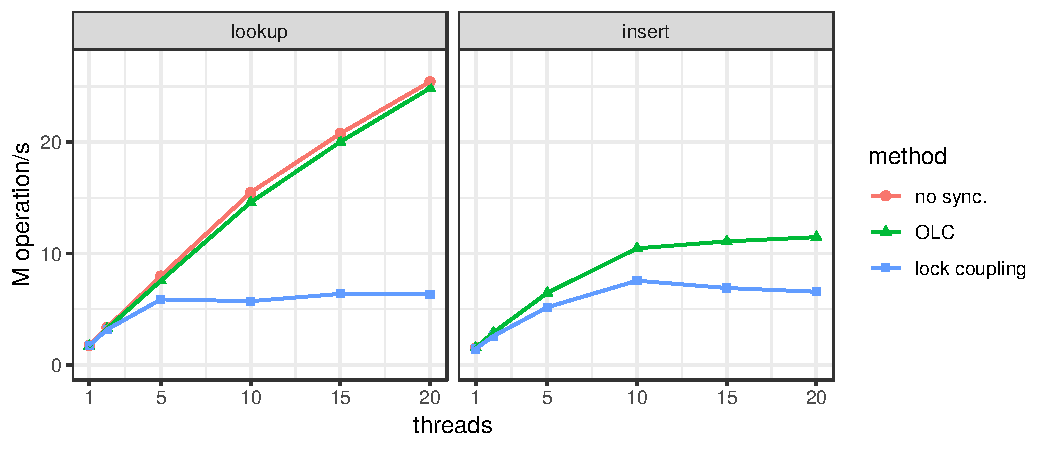
\includegraphics[width=\linewidth]{scale.pdf}
  \vspace{0.2cm}
  \caption{Scalability on 10-core system for B-tree operations (100M values).}
  \label{fig:scale}
\end{figure}

As Figure~\ref{fig:scale} shows, the results change dramatically once we use multiple threads.
For lookup, the scalability of OLC is near-linear up to 20 threads, even though the system has only 10 ``real cores''.
The OLC scalability for insert is also respectable (though not quite as linear because multi-threaded insertion approaches the memory bandwidth of our processor).
The figure also shows that the results of traditional lock coupling with read/write locks are significantly worse than OLC.
With 20 threads, lookup with OLC is 3.9$\times$ faster than traditional lock coupling.

\section{Summary}\label{sec:conc}

Optimistic Lock Coupling (OLC) is an effective synchronization method that combines the simplicity of traditional lock coupling with the superior scalability of lock-free approaches.
OLC is widely applicable and has already been successfully used to synchronize several data structures, including B-trees, binary search trees, and different trie variants.
These features make it highly attractive for modern database systems as well as performance-critical systems software in general.

\begin{thebibliography}{10}

\bibitem{DBLP:conf/spaa/BalmauGHZ16}
O.~Balmau, R.~Guerraoui, M.~Herlihy, and I.~Zablotchi.
\newblock Fast and robust memory reclamation for concurrent data structures.
\newblock In {\em SPAA}, 2016.

\bibitem{DBLP:journals/acta/BayerS77}
R.~Bayer and M.~Schkolnick.
\newblock Concurrency of operations on {B}-trees.
\newblock {\em Acta Informatica}, 9, 1977.

\bibitem{hot}
R.~Binna, E.~Zangerle, M.~Pichl, G.~Specht, and V.~Leis.
\newblock {HOT}: A height optimized trie index for main-memory database
  systems.
\newblock In {\em SIGMOD}, 2018.

\bibitem{DBLP:conf/ppopp/BronsonCCO10}
N.~G. Bronson, J.~Casper, H.~Chafi, and K.~Olukotun.
\newblock A practical concurrent binary search tree.
\newblock In {\em PPOPP}, 2010.

\bibitem{DBLP:conf/vldb/ChaHKK01}
S.~K. Cha, S.~Hwang, K.~Kim, and K.~Kwon.
\newblock Cache-conscious concurrency control of main-memory indexes on
  shared-memory multiprocessor systems.
\newblock In {\em VLDB}, 2001.

\bibitem{intel}
I.~Cutress.
\newblock {Intel} goes for 48-cores: {Cascade-AP} with multi-chip package
  coming soon.
\newblock
  \url{https://www.anandtech.com/show/13535/intel-goes-for-48cores-cascade-ap},
  2018 (accessed January, 2019).

\bibitem{DBLP:conf/cidr/FaleiroA17}
J.~M. Faleiro and D.~J. Abadi.
\newblock Latch-free synchronization in database systems: Silver bullet or
  fool's gold?
\newblock In {\em CIDR}, 2017.

\bibitem{DBLP:journals/ftdb/Graefe11}
G.~Graefe.
\newblock Modern {B}-tree techniques.
\newblock {\em Foundations and Trends in Databases}, 3(4), 2011.

\bibitem{DBLP:conf/hpca/KarnagelDRLLSL14}
T.~Karnagel, R.~Dementiev, R.~Rajwar, K.~Lai, T.~Legler, B.~Schlegel, and
  W.~Lehner.
\newblock Improving in-memory database index performance with
  {Intel}\({}^{\mbox{{\textregistered}}}\) transactional synchronization
  extensions.
\newblock In {\em HPCA}, 2014.

\bibitem{DBLP:journals/tods/LehmanY81}
P.~L. Lehman and S.~B. Yao.
\newblock Efficient locking for concurrent operations on {B}-trees.
\newblock {\em {ACM} Trans. Database Syst.}, 6(4), 1981.

\bibitem{leanstore}
V.~Leis, M.~Haubenschild, A.~Kemper, and T.~Neumann.
\newblock Leanstore: In-memory data management beyond main memory.
\newblock In {\em ICDE}, 2018.

\bibitem{art}
V.~Leis, A.~Kemper, and T.~Neumann.
\newblock The adaptive radix tree: {ARTful} indexing for main-memory databases.
\newblock In {\em ICDE}, 2013.

\bibitem{htmtkde}
V.~Leis, A.~Kemper, and T.~Neumann.
\newblock Scaling {HTM}-supported database transactions to many cores.
\newblock {\em {IEEE} Trans. Knowl. Data Eng.}, 28(2), 2016.

\bibitem{artsync}
V.~Leis, F.~Scheibner, A.~Kemper, and T.~Neumann.
\newblock The {ART} of practical synchronization.
\newblock In {\em DaMoN}, 2016.

\bibitem{DBLP:conf/icde/LevandoskiLS13a}
J.~J. Levandoski, D.~B. Lomet, and S.~Sengupta.
\newblock The {Bw}-tree: A {B}-tree for new hardware platforms.
\newblock In {\em ICDE}, 2013.

\bibitem{DBLP:journals/pvldb/MakreshanskiLS15}
D.~Makreshanski, J.~J. Levandoski, and R.~Stutsman.
\newblock To lock, swap, or elide: On the interplay of hardware transactional
  memory and lock-free indexing.
\newblock {\em {PVLDB}}, 8(11), 2015.

\bibitem{DBLP:dblp_conf/eurosys/MaoKM12}
Y.~Mao, E.~Kohler, and R.~T. Morris.
\newblock Cache craftiness for fast multicore key-value storage.
\newblock In {\em EuroSys}, 2012.

\bibitem{DBLP:journals/tpds/Michael04}
M.~M. Michael.
\newblock Hazard pointers: Safe memory reclamation for lock-free objects.
\newblock {\em {IEEE} Trans. Parallel Distrib. Syst.}, 15(6), 2004.

\bibitem{DBLP:journals/jacm/ShalevS06}
O.~Shalev and N.~Shavit.
\newblock Split-ordered lists: Lock-free extensible hash tables.
\newblock {\em J. {ACM}}, 53(3), 2006.

\bibitem{amd}
A.~Shilov.
\newblock {AMD} previews {EPYC} ‘{Rome}’ processor: Up to 64 {Zen} 2 cores.
\newblock
  \url{https://www.anandtech.com/show/13561/amd-previews-epyc-rome-processor-up-to-64-zen-2-cores},
  2018 (accessed January, 2019).

\bibitem{DBLP:conf/sosp/TuZKLM13}
S.~Tu, W.~Zheng, E.~Kohler, B.~Liskov, and S.~Madden.
\newblock Speedy transactions in multicore in-memory databases.
\newblock In {\em SOSP}, 2013.

\bibitem{buzzword}
Z.~Wang, A.~Pavlo, H.~Lim, V.~Leis, H.~Zhang, M.~Kaminsky, and D.~Andersen.
\newblock Building a {Bw}-tree takes more than just buzz words.
\newblock In {\em SIGMOD}, 2018.

\end{thebibliography}


%\bibliographystyle{abbrv}
%\bibliography{main}

\end{document}

\end{article}

\begin{article}
{\textsc{ReFIT}: Reranker Relevance Feedback during Inference}
{Revanth Gangi Reddy, Pradeep Dasigi, Md Arafat Sultan, Arman Cohan, Avirup Sil, Heng Ji, Hannaneh Hajishirzi}
\setcounter{section}{0}
\pdfminorversion=5
\documentclass[11pt]{article}
\usepackage{deauthor,times,graphicx,caption,microtype}
\usepackage{hyperref}
\usepackage{listings}
\usepackage{booktabs}

\begin{document}

\title{Optimistic Lock Coupling: A Scalable and Efficient General-Purpose Synchronization Method}

\author{Viktor Leis, Michael Haubenschild\raisebox{0.9ex}{$\ast$}, Thomas Neumann\\ Technische Universit{\"a}t M{\"u}nchen \hspace{0.7cm} Tableau Software\raisebox{0.9ex}{$\ast$} \\ {\{leis,neumann\}{@}in.tum.de} \hspace{0.7cm} {mhaubenschild{@}tableau.com\raisebox{0.9ex}{$\ast$}}}

\maketitle

\begin{abstract}
As the number of cores on commodity processors continues to increase, scalability becomes more and more crucial for overall performance.
Scalable and efficient concurrent data structures are particularly important, as these are often the building blocks of parallel algorithms.
Unfortunately, traditional synchronization techniques based on fine-grained locking have been shown to be unscalable on modern multi-core CPUs.
Lock-free data structures, on the other hand, are extremely difficult to design and often incur significant overhead.

In this work, we make the case for Optimistic Lock Coupling as a practical alternative to both traditional locking and the lock-free approach.
We show that Optimistic Lock Coupling is highly scalable and almost as simple to implement as traditional lock coupling.
Another important advantage is that it is easily applicable to most tree-like data structures.
We therefore argue that Optimistic Lock Coupling, rather than a complex and error-prone custom synchronization protocol, should be the default choice for performance-critical data structures.
\end{abstract}

\section{Introduction}

% more and more cores
Today, Intel's commodity server processors have up to 28 cores and its upcoming microarchitecture will have up to 48 cores per socket~\cite{intel}.
Similarly, AMD currently stands at 32 cores and this number is expected to double in the next generation~\cite{amd}.
Since both platforms support simultaneous multithreading (also known as hyperthreading), affordable commodity servers (with up to two sockets) will soon routinely have between 100 and 200 hardware threads.

% data structure scalability is important
With such a high degree of hardware parallelism, efficient data processing crucially depends on how well concurrent data structures scale.
Internally, database systems use a plethora of data structures like table heaps, internal work queues, and, most importantly, index structures.
Any of these can easily become a scalability (and therefore overall performance) bottleneck on many-core CPUs.

% traditional synchronization: fine-grained locks, slow, cache invalidation
Traditionally, database systems synchronize internal data structures using fine-grained reader/writer locks\footnote{In this work, we focus on data structure synchronization rather than high-level transaction semantics and therefore use the term {\em lock} for what would typically be called {\em latch} in the database literature. We thus follow common computer science (rather than database) terminology.}.
Unfortunately, while fine-grained locking makes lock contention unlikely, it still results in bad scalability because lock acquisition and release require writing to shared memory.
Due to the way cache coherency is implemented on modern multi-core CPUs, these writes cause additional cache misses\footnote{The cache coherency protocol ensures that all copies of a cache line on other cores are invalidated before the write can proceed.} and the cache line containing the lock's internal data becomes a point of physical contention.
As a result, any frequently-accessed lock (e.g., the lock of the root node of a B-tree) severely limits scalability.

% lock-free bw-tree: no more latches, but indirections, extremely complex
Lock-free data structures like the Bw-tree~\cite{DBLP:conf/icde/LevandoskiLS13a} (a lock-free B-tree variant) or the Split-Ordered List~\cite{DBLP:journals/jacm/ShalevS06} (a lock-free hash table) do not acquire any locks and therefore generally scale much better than locking-based approaches (in particular for read-mostly workloads).
However, lock-free synchronization has other downsides:
First, it is very difficult and results in extremely complex and error-prone code (when compared to locking).
Second, because the functionality of atomic primitives provided by the hardware (e.g., atomically compare-and-swap 8 bytes) is limited, complex operations require additional indirections within the data structure.
For example, the Bw-tree requires an indirection table and the Split-Ordered List requires ``dummy nodes'', resulting in overhead due to additional cache misses.

% OLC for the win
In this paper we make the case for {\em Optimistic Lock Coupling (OLC)}, a synchronization method that combines some of the best properties of lock-based and lock-free synchronization.
OLC utilizes a special lock type that can be used in two modes:
The first mode is similar to a traditional mutex and excludes other threads by physically acquiring the underlying lock.
In the second mode, reads can proceed optimistically by validating a version counter that is embedded in the lock (similar to optimistic concurrency control).
The first mode is typically used by writers and the second mode by readers.
Besides this special lock type, OLC is based on the observation that optimistic lock validations can be interleaved/coupled---similar to the pair-wise interleaved lock acquisition of traditional lock coupling.
Hence, the name Optimistic Lock Coupling.

OLC has a number of desirable features:
\begin{itemize}
\item By reducing the number of writes to shared memory locations and thereby avoiding cache invalidations, it {\bf scales well} for most workloads.
\item In comparison to unsynchronized code, it requires few additional CPU instructions making it {\bf efficient}.
\item OLC is {\bf widely applicable} to different data structures. It has already been successfully used for synchronizing binary search trees~\cite{DBLP:conf/ppopp/BronsonCCO10}, tries~\cite{artsync}, trie/B-tree hybrids~\cite{DBLP:dblp_conf/eurosys/MaoKM12}, and B-trees~\cite{buzzword}.
\item In comparison to the lock-free paradigm, it is also {\bf easy to use} and requires few modifications to existing, single-threaded data structures.
\end{itemize}
Despite these positive features and its simplicity, OLC is not yet widely known.
The goal of this paper is therefore to popularize this simple idea and to make a case for it.
We argue that OLC deserves to be widely known.
It is a good default synchronization paradigm---more complex, data structure-specific protocols are seldom beneficial.

The rest of the paper is organized as follows.
Section~\ref{sec:related} discusses related work, tracing the history of OLC and its underlying ideas in the literature.
The core of the paper is Section~\ref{sec:olc}, which describes the ideas behind OLC and how it can be used to synchronize complex data structures.
In Section~\ref{sec:evaluation} we experimentally show that OLC has low overhead and scales well when used to synchronize an in-memory B-tree.
We summarize the paper in Section~\ref{sec:conc}.

\newpage
\section{Related Work}\label{sec:related}

Lock coupling has been proposed as a method for allowing concurrent operations on B-trees in 1977~\cite{DBLP:journals/acta/BayerS77}.
This traditional and still widely-used method, described in detail in Graefe's B-tree survey~\cite{DBLP:journals/ftdb/Graefe11}, is also called ``latch coupling'', ``hand-over-hand locking'', and ``crabbing''.
Because at most two locks are held at-a-time during tree traversal, this technique seemingly allows for a high degree of parallelism---in particular if read/write locks are used to enable inner nodes to be locked in shared mode.
However, as we show in Section~\ref{sec:evaluation}, on modern hardware lock acquisition (even in shared mode) results in suboptimal scalability.

An early alternative from 1981 is a B-tree variant called B-link tree~\cite{DBLP:journals/tods/LehmanY81}, which only holds a single lock at a time.
It is based on the observation that between the release of the parent lock and the acquisition of the child lock, the only ``dangerous'' thing that could have happened is the split of a child node (assuming one does not implement merge operations).
Thus, when a split happens, the key being searched might end up on a neighboring node to the right of the current child node.
A B-link tree traversal therefore detects this condition and, if needed, transparently proceeds to the neighboring node.
Releasing the parent lock early is highly beneficial when the child node needs to be fetched from disk.
For in-memory workloads, however, the B-link tree has the same scalability issues as lock coupling (it acquires just as many locks).

The next major advance, Optimistic Latch-Free Index Traversal (OLFIT)~\cite{DBLP:conf/vldb/ChaHKK01}, was proposed in 2001.
OLFIT introduced the idea of a combined lock/update counter, which we call {\em optimistic lock}. % , for lack of a better name,
Based on these per-node optimistic locks and the synchronization protocol of the B-link tree, OLFIT finally achieves good scalability on parallel processors.
The OLFIT protocol is fairly complex, as it requires both the non-trivial B-link protocol and optimistic locks.
Furthermore, like the B-link tree protocol, it does not support merging nodes, and is specific to B-trees (cannot easily be applied to other data structures).

In the following two decades, the growth of main-memory capacity led to much research into other data structures besides the venerable B-tree.
Particularly relevant for our discussion is Bronson et al.'s~\cite{DBLP:conf/ppopp/BronsonCCO10} concurrent binary search tree, which is based on optimistic version validation and has a sophisticated, data structure-specific synchronization protocol.
To the best of our knowledge, this 2010 paper is the first that, as part of its protocol, interleaves version validation across nodes---rather than validating each node separately like OLFIT.
In that paper, this idea is called ``hand-over-hand, optimistic validation'', while we prefer the term Optimistic Lock Coupling to highlight the close resemblance to traditional lock coupling.
Similarly, Mao et al.'s~\cite{DBLP:dblp_conf/eurosys/MaoKM12} Masstree (a concurrent hybrid trie/B-tree) is also based on the same ideas, but again uses them as part of a more complex protocol.

The Adaptive Radix Tree (ART)~\cite{art} is another recent in-memory data structure, which we proposed in 2013.
In contrast to the two data structures just mentioned, it was originally designed with single-threaded performance in mind without supporting concurrency.
To add support for concurrency, we initially started designing a custom protocol called Read-Optimized Write Exclusion (ROWEX)~\cite{artsync}, which turned out to be non-trivial and requires modifications of the underlying data structure\footnote{Note that ROWEX is already easier to apply to existing data structures than the lock-free approach. The difficulty depends on the data structure. Applying ROWEX is hard for B-trees with sorted keys and fairly easy for copy-on-write data structures like the Height Optimized Trie~\cite{hot}---with ART being somewhere in the middle.}.
However, fairly late in the project, we also realized, that OLC {\em alone} (rather than as part of a more complex protocol) is sufficient to synchronize ART.
No other changes to the data structure were necessary.
Both approaches were published and experimentally evaluated in a followup paper~\cite{artsync}, which shows that, despite its simplicity, OLC is efficient, scalable, and generally outperforms ROWEX.

Similar results were recently published regarding B-trees~\cite{buzzword}.
In this experimental study a simple OLC-based synchronization outperformed the Bw-tree~\cite{DBLP:conf/icde/LevandoskiLS13a}, a complex lock-free synchronization approach.
Another recent paper shows that for write-intensive workloads, locking often performs better than lock-free synchronization~\cite{DBLP:conf/cidr/FaleiroA17}.
These experiences indicate that OLC is a general-purpose synchronization paradigm and motivate the current paper.

%foster b-tree\cite{DBLP:journals/tods/GraefeKK12}
%Shasha theory~\cite{DBLP:journals/tods/ShashaG88}

\section{Optimistic Lock Coupling}\label{sec:olc}

% locks suck
The standard technique for inter-thread synchronization is mutual exclusion using fine-grained locks.
In a B-tree, for example, every node usually has its own associated lock, which is acquired before accessing that node.
The problem of locking on modern multi- and many-core processors is that lock acquisition and release require writing to the shared memory location that implements the lock.
This write causes exclusive ownership of the underlying cache line and invalidates copies of it on all other processor cores.
For hierarchical, tree-like data structures, the lock of the root node becomes a point of physical contention---even in read-only workloads and even when read/write locks are used.
Depending on the specific data structure, number of cores, cache coherency protocol implementation, cache topology, whether Non-Uniform Memory Access (NUMA) is used, locking can even result in multi-threaded performance that is worse than single-threaded execution.

% in b-trees this happens very much
The inherent pessimism of locking is particularly unfortunate for B-trees:
Despite the fact that logical modifications of the root node are very infrequent, every B-tree operation must lock the root node during tree traversal\footnote{To a lesser extent this obviously applies to all inner nodes, not just the root.}.
Even the vast majority of update operations (with the exception of splits and merges), only modify a single leaf node.
These observations indicate that a more optimistic approach, which does not require locking inner nodes, would be very beneficial for B-trees.

\subsection{Optimistic Locks}

% optimism to the rescue
As the name indicates, optimistic locks try to solve the scalability issues of traditional locks using an optimistic approach.
Instead of always physically acquiring locks, even for nodes that are unlikely to be modified simultaneously, after-the-fact validation is used to detect conflicts.
This is done by augmenting each lock with a version/update counter that is incremented on every modification.
Using this version counter, readers can optimistically proceed before validating that the version did not change to ensure that the read was safe.
If validation fails, the operation is restarted.

% details on opt locks
Using optimistic locks, a read-only node access (i.e., the majority of all operations in a B-tree) does not acquire the lock and does not increment the version counter.
Instead, it performs the following steps:
\begin{enumerate}
\item read lock version (restart if lock is not free)
\item access node
\item read the version again and validate that it has not changed in the meantime
\end{enumerate}
If the last step (the validation) fails, the operation has to be restarted.
Write operations, on the other hand, are more similar to traditional locking:
\begin{enumerate}
\item acquire lock (wait if necessary)
\item access/write to node
\item increment version and unlock node
\end{enumerate}
Writes can therefore protect a node from other writes.

% similar to locks
As we observed in an earlier paper~\cite{artsync}, because of similar semantics, optimistic locks can be hidden behind an API very similar to traditional read/write locks.
Both approaches have an exclusive lock mode, and acquiring a traditional lock in shared mode is analogous to optimistic version validation.
Furthermore, like with some implementations of traditional read/write locks, optimistic locks allow upgrading a shared lock to an exclusive lock.
Lock upgrades are, for example, used to avoid most B-tree update operations from having to lock inner nodes.
In our experience, the close resemblance of optimistic and traditional locks simplifies the reasoning about optimistic locks;
one can apply similar thinking as in traditional lock-based protocols.

\subsection{Lock Coupling with Optimistic Locks}

\begin{figure}
  \centering
  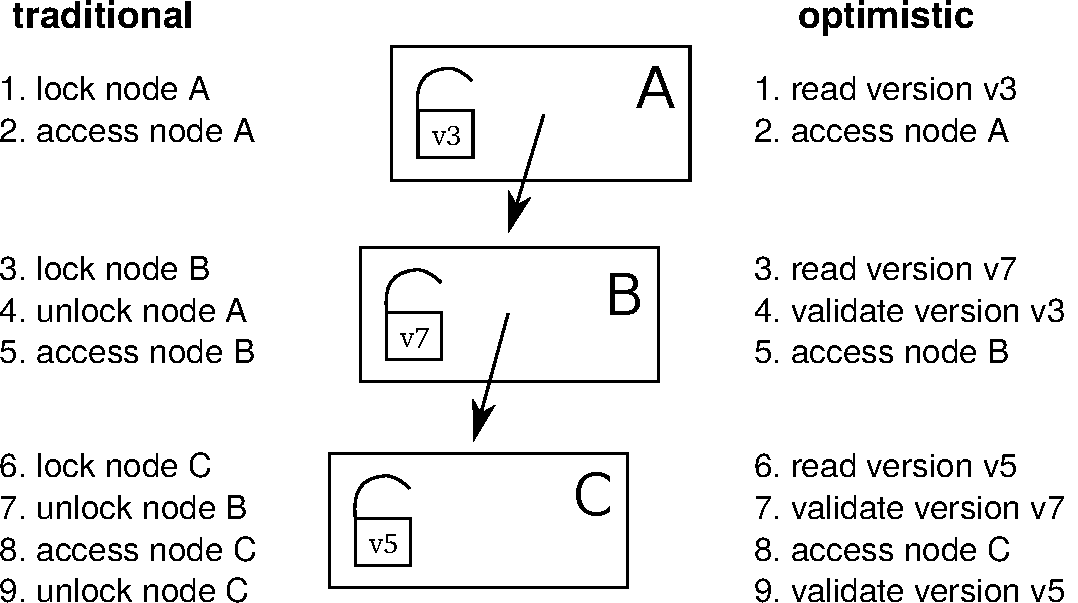
\includegraphics[width=0.65\linewidth]{olcall.pdf}
  \vspace{0.2cm}
  \caption{Comparison of a lookup operation in a 3-level tree using traditional lock coupling (left-hand side) vs.~optimistic lock coupling (right-hand side).}
  \label{fig:olc}
\end{figure}

The traditional and most common lock-based synchronization protocol for B-trees is lock coupling, which interleaves lock acquisitions while holding at most two locks at a time.
If, as we observed earlier, optimistic locks have similar semantics as traditional locks, it is natural to ask whether lock coupling can be combined with optimistic locks.
And indeed the answer is yes: One can almost mechanically translate traditional lock coupling code to optimistic lock coupling code.
This is illustrated in Figure~\ref{fig:olc}, which compares the traversal in a tree of height 3 using traditional and optimistic locks.
As the figure shows, the main difference is that locking is translated to reading the version and that unlocking becomes validation of the previously read version.
This simple change provides efficient lock-free tree traversal without the need to design a complex synchronization protocol.

It is important to emphasize the conceptual simplicity of OLC in comparison to data structures that use custom protocols like the Bw-tree~\cite{DBLP:conf/icde/LevandoskiLS13a}.
To implement lock-free access, the Bw-tree requires an indirection table, delta nodes, complex splitting and merging logic, retry logic, etc.
OLC, on the other hand, can directly be applied to B-trees mostly by adding the appropriate optimistic locking code and without modifying the node layout itself.
Therefore, OpenBw-Tree, an open source implementation of the Bw-tree, requires an order of magnitude more code than a B-tree based on OLC\footnote{Both implementations are available on GitHub: \url{https://github.com/wangziqi2016/index-microbench}}.
Given how difficult it is to develop, validate, and debug lock-free code, simplicity is obviously a major advantage.

\subsection{Correctness Aspects}

\begin{figure}
  % \centering
  %[basicstyle=\normalsize\ttfamily,showstringspaces=false,columns=fullflexible,breaklines=false,breakatwhitespace=true,numbers=none,numberstyle=\small,style=C,keepspaces=true]
\begin{lstlisting}[basicstyle=\ttfamily,language=C++,numbers=left,numberstyle=\small]
std::atomic<BTreeNode*> root;

// search for key in B+tree, returns payload in resultOut
bool lookup(Key key, Value& resultOut) {
   BTreeNode* node = root.load();
   uint64_t nodeVersion = node->readLockOrRestart();
   if (node != root.load()) // make sure the root is still the root
      restart();

   BTreeInner<Key>* parent = nullptr;
   uint64_t parentVersion = 0;

   while (node->isInner()) {
      auto inner = (BTreeInner*)node;

      // unlock parent and make current node the parent
      if (parent)
         parent->readUnlockOrRestart(parentVersion);
      parent = inner;
      parentVersion = nodeVersion;

      // search for next node
      node = inner->findChild(key);
      // validate 'inner' to ensure that 'node' pointer is valid
      inner->checkOrRestart(nodeVersion);
      // now it safe to dereference 'node' pointer (read its version)
      nodeVersion = node->readLockOrRestart();
   }

   // search in leaf and retrieve payload
   auto leaf = (BTreeLeaf*)node;
   bool success = leaf->findValue(key, resultOut);

   // unlock everything
   if (parent)
      parent->readUnlockOrRestart(parentVersion);
   node->readUnlockOrRestart(nodeVersion);

   return success;
}
\end{lstlisting}
  \vspace{0.2cm}
  \caption{B-tree lookup code using OLC. For simplicity, the restart logic is not shown.}
  \label{fig:lookup}
\end{figure}

So far, we have introduced the high-level ideas behind OLC and have stressed its similarity to traditional lock coupling.
Let us now discuss some cases where the close similarity between lock coupling and OLC breaks down.
To make this more concrete, we show the B-tree lookup code in Figure~\ref{fig:lookup}.
In the code, \texttt{readLockOrRestart} reads the lock version and \texttt{readUnlockOrRestart} validates that the read was correct.

One issue with OLC is that any pointer speculatively read from a node may point to invalid memory (if that node is modified concurrently).
Dereferencing such a pointer (e.g., to read its optimistic lock), may cause a segmentation fault or undefined behavior.
In the code shown in Figure~\ref{fig:lookup}, this problem is prevented by the extra check in line 25, which ensures that the read from the node containing the pointer was correct.
Without this additional validation, the code would in line 27 dereference the pointer speculatively read in line 23.
Note that the implementation of \texttt{checkOrRestart} is actually identical to \texttt{readUnlockOrRestart}.
We chose to give it a different name to highlight the fact that this extra check would not be necessary with read/write locks.

Another potential issue with optimistic locks is code that does not terminate.
Code that speculatively accesses a node, like an intra-node binary search, should be written in a way such that it always terminates---even in the presence of concurrent writes.
Otherwise, the validation code that detects the concurrent write will never run.
The binary search of a B-tree, for example, needs to be written in such a way that each comparison makes progress.
For some data structures that do not require loops in the traversal code (like ART) termination is trivially true.

\subsection{Implementation Details}

% implementation, efficiency
To implement an optimistic lock, one can combine the lock and the version counter into a single 64-bit\footnote{Even after subtracting one bit for the lock status, a back-of-the-envelope calculation can show that 63 bits are large enough to never overflow in practice.} word~\cite{artsync}.
A typical read operation will therefore merely consist of reading this version counter atomically.
In C++11 this can be implemented using the \texttt{std::atomic} type.

On x86, atomic reads are cheap because of x86's strong memory order guarantees.
No memory fences are required for sequentially-consistent loads, which are translated (by both GCC and clang) into standard \texttt{MOV} instructions.
Hence, the only effect of \texttt{std::atomic} for loads is preventing instruction re-ordering.
This makes version access and validation cheap.
Acquiring and releasing an optimistic lock in exclusive mode has comparable cost to a traditional lock:
A fairly expensive sequentially-consistent store is needed for acquiring a lock, while a standard \texttt{MOV} suffices for releasing it.
A simple sinlock-based implementation of optimistic locks can be found in the appendix of an earlier paper~\cite{artsync}.

OLC code must be able to handle restarts since validation or lock upgrade can fail due to concurrent writers.
Restarts can easily be implemented by wrapping the data structure operation in a loop (for simplicity not shown in Figure~\ref{fig:lookup}).
Such a loop also enables limiting the number of optimistic retry operations and falling back to pessimistic locking in cases of very heavy contention.
The ability to fall back to traditional locking is a major advantage of OLC in terms of robustness over lock-free approaches, which do not have this option.

In addition to the optimistic shared mode and the exclusive mode, optimistic locks also support a ``shared pessimistic'' mode, which physically acquires the lock in shared mode (allowing multiple concurrent readers but no writers).
This mode is useful for table (or range) scans that touch many tuples on a leaf page (which would otherwise easily abort).
Finally, let us mention that large range scans and table scans, should be broken up into several per-node traversals as is done in the LeanStore~\cite{leanstore} system.

Like all lock-free data structures, but unlike traditional locking and Hardware Transactional Memory~\cite{DBLP:conf/hpca/KarnagelDRLLSL14,DBLP:journals/pvldb/MakreshanskiLS15,htmtkde}, OLC requires care when deleting (and reusing) nodes.
The reason is that a deleting thread can never be sure that a node can be reclaimed because other threads might still be optimistically reading from that node.
Therefore, standard solutions like epoch-based reclamation~\cite{DBLP:conf/sosp/TuZKLM13}, hazard pointers~\cite{DBLP:journals/tpds/Michael04}, or optimized hazard pointers~\cite{DBLP:conf/spaa/BalmauGHZ16} need to be used.
These memory reclamation techniques are, however, largely orthogonal to the synchronization protocol itself.

%-lock-free is not a strong guarantee

\newpage
\section{Evaluation}\label{sec:evaluation}

Let us now experimentally evaluate the overhead and scalability of OLC.
For the experiments, we use an in-memory B+tree implemented in C++11 using templates, which is configured to use nodes of 4096 bytes, random 8 byte keys, and 8 byte payloads.
Based on this B-tree, we compare the following synchronization approaches:
\begin{itemize}
\item an OLC implementation\footnote{An almost identical OLC implementation is available on github: \url{https://github.com/wangziqi2016/index-microbench/tree/master/BTreeOLC}}
\item a variant based on traditional lock coupling and read/write locks
\item the unsynchronized B-tree, which obviously is only correct for read-only workloads but allows measuring the overhead of synchronization
\end{itemize}
Note that earlier work has compared the OLC implementation with a Bw-tree implementation~\cite{buzzword} and other state-of-the-art in-memory index structures.

We use a Haswell EP system with an Intel Xeon E5-2687W v3 CPU, which has 10 cores (20 ``Hyper-Threads'') and 25~MB of L3 cache.
The system is running Ubuntu 18.10 and we use GCC 8.2.0 to compile our code.
The CPU counters are obtained using the Linux perf API\footnote{We use the following convenience wrapper: \url{https://github.com/viktorleis/perfevent}}.

\begin{table}
  \caption{Performance and CPU counters for lookup and insert operations in a B-tree with 100M keys. We perform 100M operations and normalize the CPU counters by that number.}
  \label{tab:overhead}
  \centering
  \begin{tabular}{lrrrrrrr}\toprule
                    &         &        &        & instruc-  & L1     & L3     & branch \\
                    & threads & M op/s & cycles & tions & misses & misses & misses \\\midrule
lookup (no sync.)   & 1       & 1.72   & 2028   & 283     & 39.1   & 14.9   & 16.1   \\
lookup (OLC)        & 1       & 1.65   & 2107   & 370     & 43.9   & 15.1   & 16.7   \\
lookup (lock coup.) & 1       & 1.72   & 2078   & 365     & 42.3   & 16.9   & 15.7   \\\midrule
insert (no sync.)   & 1       & 1.51   & 2286   & 530     & 59.8   & 31.1   & 17.3   \\
insert (OLC)        & 1       & 1.50   & 2303   & 629     & 61.2   & 31.1   & 16.5   \\
insert (lock coup.) & 1       & 1.41   & 2473   & 644     & 61.0   & 31.0   & 17.2   \\\midrule
lookup (no sync.)   & 10      & 15.48  & 2058   & 283     & 38.6   & 15.5   & 16.0   \\
lookup (OLC)        & 10      & 14.60  & 2187   & 370     & 43.8   & 15.8   & 16.8   \\
lookup (lock coup.) & 10      & 5.71   & 5591   & 379     & 54.2   & 17.0   & 14.8   \\\midrule
insert (no sync.)   & 10      & -      & -      & -       & -      & -      & -      \\
insert (OLC)        & 10      & 10.46  & 2940   & 656     & 62.0   & 32.5   & 16.8   \\
insert (lock coup.) & 10      & 7.55   & 4161   & 667     & 75.0   & 28.6   & 16.2   \\
    \bottomrule
\end{tabular}
\end{table}

Table~\ref{tab:overhead} compares the performance and CPU counters for lookup and insert operations in a B-tree with 100M keys.
With {\em single-threaded} execution, we observe that all three approaches have very similar performance.
Adding traditional or optimistic locks to unsynchronized B-tree code results in up to 30\% of additional instructions without affecting single-threaded performance much.

\begin{figure}
  \centering
  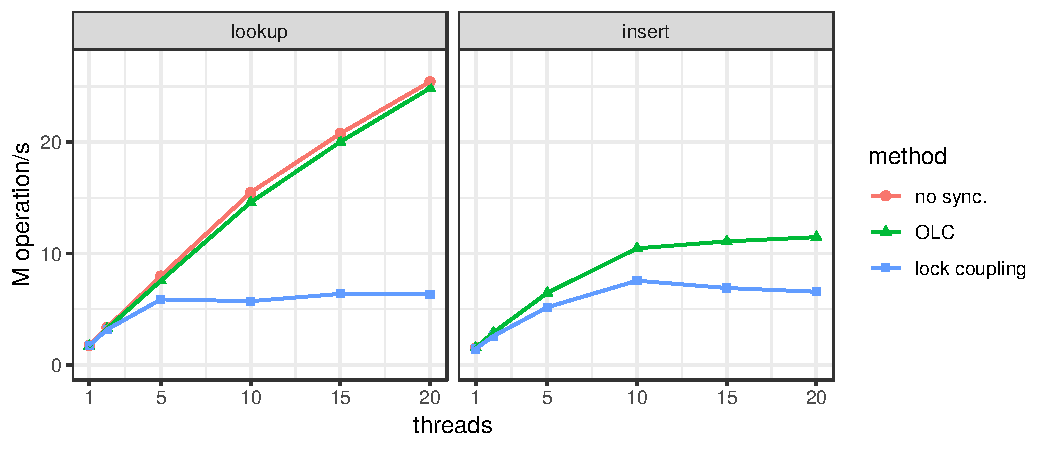
\includegraphics[width=\linewidth]{scale.pdf}
  \vspace{0.2cm}
  \caption{Scalability on 10-core system for B-tree operations (100M values).}
  \label{fig:scale}
\end{figure}

As Figure~\ref{fig:scale} shows, the results change dramatically once we use multiple threads.
For lookup, the scalability of OLC is near-linear up to 20 threads, even though the system has only 10 ``real cores''.
The OLC scalability for insert is also respectable (though not quite as linear because multi-threaded insertion approaches the memory bandwidth of our processor).
The figure also shows that the results of traditional lock coupling with read/write locks are significantly worse than OLC.
With 20 threads, lookup with OLC is 3.9$\times$ faster than traditional lock coupling.

\section{Summary}\label{sec:conc}

Optimistic Lock Coupling (OLC) is an effective synchronization method that combines the simplicity of traditional lock coupling with the superior scalability of lock-free approaches.
OLC is widely applicable and has already been successfully used to synchronize several data structures, including B-trees, binary search trees, and different trie variants.
These features make it highly attractive for modern database systems as well as performance-critical systems software in general.

\begin{thebibliography}{10}

\bibitem{DBLP:conf/spaa/BalmauGHZ16}
O.~Balmau, R.~Guerraoui, M.~Herlihy, and I.~Zablotchi.
\newblock Fast and robust memory reclamation for concurrent data structures.
\newblock In {\em SPAA}, 2016.

\bibitem{DBLP:journals/acta/BayerS77}
R.~Bayer and M.~Schkolnick.
\newblock Concurrency of operations on {B}-trees.
\newblock {\em Acta Informatica}, 9, 1977.

\bibitem{hot}
R.~Binna, E.~Zangerle, M.~Pichl, G.~Specht, and V.~Leis.
\newblock {HOT}: A height optimized trie index for main-memory database
  systems.
\newblock In {\em SIGMOD}, 2018.

\bibitem{DBLP:conf/ppopp/BronsonCCO10}
N.~G. Bronson, J.~Casper, H.~Chafi, and K.~Olukotun.
\newblock A practical concurrent binary search tree.
\newblock In {\em PPOPP}, 2010.

\bibitem{DBLP:conf/vldb/ChaHKK01}
S.~K. Cha, S.~Hwang, K.~Kim, and K.~Kwon.
\newblock Cache-conscious concurrency control of main-memory indexes on
  shared-memory multiprocessor systems.
\newblock In {\em VLDB}, 2001.

\bibitem{intel}
I.~Cutress.
\newblock {Intel} goes for 48-cores: {Cascade-AP} with multi-chip package
  coming soon.
\newblock
  \url{https://www.anandtech.com/show/13535/intel-goes-for-48cores-cascade-ap},
  2018 (accessed January, 2019).

\bibitem{DBLP:conf/cidr/FaleiroA17}
J.~M. Faleiro and D.~J. Abadi.
\newblock Latch-free synchronization in database systems: Silver bullet or
  fool's gold?
\newblock In {\em CIDR}, 2017.

\bibitem{DBLP:journals/ftdb/Graefe11}
G.~Graefe.
\newblock Modern {B}-tree techniques.
\newblock {\em Foundations and Trends in Databases}, 3(4), 2011.

\bibitem{DBLP:conf/hpca/KarnagelDRLLSL14}
T.~Karnagel, R.~Dementiev, R.~Rajwar, K.~Lai, T.~Legler, B.~Schlegel, and
  W.~Lehner.
\newblock Improving in-memory database index performance with
  {Intel}\({}^{\mbox{{\textregistered}}}\) transactional synchronization
  extensions.
\newblock In {\em HPCA}, 2014.

\bibitem{DBLP:journals/tods/LehmanY81}
P.~L. Lehman and S.~B. Yao.
\newblock Efficient locking for concurrent operations on {B}-trees.
\newblock {\em {ACM} Trans. Database Syst.}, 6(4), 1981.

\bibitem{leanstore}
V.~Leis, M.~Haubenschild, A.~Kemper, and T.~Neumann.
\newblock Leanstore: In-memory data management beyond main memory.
\newblock In {\em ICDE}, 2018.

\bibitem{art}
V.~Leis, A.~Kemper, and T.~Neumann.
\newblock The adaptive radix tree: {ARTful} indexing for main-memory databases.
\newblock In {\em ICDE}, 2013.

\bibitem{htmtkde}
V.~Leis, A.~Kemper, and T.~Neumann.
\newblock Scaling {HTM}-supported database transactions to many cores.
\newblock {\em {IEEE} Trans. Knowl. Data Eng.}, 28(2), 2016.

\bibitem{artsync}
V.~Leis, F.~Scheibner, A.~Kemper, and T.~Neumann.
\newblock The {ART} of practical synchronization.
\newblock In {\em DaMoN}, 2016.

\bibitem{DBLP:conf/icde/LevandoskiLS13a}
J.~J. Levandoski, D.~B. Lomet, and S.~Sengupta.
\newblock The {Bw}-tree: A {B}-tree for new hardware platforms.
\newblock In {\em ICDE}, 2013.

\bibitem{DBLP:journals/pvldb/MakreshanskiLS15}
D.~Makreshanski, J.~J. Levandoski, and R.~Stutsman.
\newblock To lock, swap, or elide: On the interplay of hardware transactional
  memory and lock-free indexing.
\newblock {\em {PVLDB}}, 8(11), 2015.

\bibitem{DBLP:dblp_conf/eurosys/MaoKM12}
Y.~Mao, E.~Kohler, and R.~T. Morris.
\newblock Cache craftiness for fast multicore key-value storage.
\newblock In {\em EuroSys}, 2012.

\bibitem{DBLP:journals/tpds/Michael04}
M.~M. Michael.
\newblock Hazard pointers: Safe memory reclamation for lock-free objects.
\newblock {\em {IEEE} Trans. Parallel Distrib. Syst.}, 15(6), 2004.

\bibitem{DBLP:journals/jacm/ShalevS06}
O.~Shalev and N.~Shavit.
\newblock Split-ordered lists: Lock-free extensible hash tables.
\newblock {\em J. {ACM}}, 53(3), 2006.

\bibitem{amd}
A.~Shilov.
\newblock {AMD} previews {EPYC} ‘{Rome}’ processor: Up to 64 {Zen} 2 cores.
\newblock
  \url{https://www.anandtech.com/show/13561/amd-previews-epyc-rome-processor-up-to-64-zen-2-cores},
  2018 (accessed January, 2019).

\bibitem{DBLP:conf/sosp/TuZKLM13}
S.~Tu, W.~Zheng, E.~Kohler, B.~Liskov, and S.~Madden.
\newblock Speedy transactions in multicore in-memory databases.
\newblock In {\em SOSP}, 2013.

\bibitem{buzzword}
Z.~Wang, A.~Pavlo, H.~Lim, V.~Leis, H.~Zhang, M.~Kaminsky, and D.~Andersen.
\newblock Building a {Bw}-tree takes more than just buzz words.
\newblock In {\em SIGMOD}, 2018.

\end{thebibliography}


%\bibliographystyle{abbrv}
%\bibliography{main}

\end{document}

\end{article}

\begin{article}
{KDD Cup CRAG competition: Systems, Findings and Learnings}
{Xiao Yang, Yifan Ethan Xu, Kai Sun, Jiaqi Wang, Lingkun Kong, Wen-tau Yih, Xin Luna Dong}
\setcounter{section}{0}
\pdfminorversion=5
\documentclass[11pt]{article}
\usepackage{deauthor,times,graphicx,caption,microtype}
\usepackage{hyperref}
\usepackage{listings}
\usepackage{booktabs}

\begin{document}

\title{Optimistic Lock Coupling: A Scalable and Efficient General-Purpose Synchronization Method}

\author{Viktor Leis, Michael Haubenschild\raisebox{0.9ex}{$\ast$}, Thomas Neumann\\ Technische Universit{\"a}t M{\"u}nchen \hspace{0.7cm} Tableau Software\raisebox{0.9ex}{$\ast$} \\ {\{leis,neumann\}{@}in.tum.de} \hspace{0.7cm} {mhaubenschild{@}tableau.com\raisebox{0.9ex}{$\ast$}}}

\maketitle

\begin{abstract}
As the number of cores on commodity processors continues to increase, scalability becomes more and more crucial for overall performance.
Scalable and efficient concurrent data structures are particularly important, as these are often the building blocks of parallel algorithms.
Unfortunately, traditional synchronization techniques based on fine-grained locking have been shown to be unscalable on modern multi-core CPUs.
Lock-free data structures, on the other hand, are extremely difficult to design and often incur significant overhead.

In this work, we make the case for Optimistic Lock Coupling as a practical alternative to both traditional locking and the lock-free approach.
We show that Optimistic Lock Coupling is highly scalable and almost as simple to implement as traditional lock coupling.
Another important advantage is that it is easily applicable to most tree-like data structures.
We therefore argue that Optimistic Lock Coupling, rather than a complex and error-prone custom synchronization protocol, should be the default choice for performance-critical data structures.
\end{abstract}

\section{Introduction}

% more and more cores
Today, Intel's commodity server processors have up to 28 cores and its upcoming microarchitecture will have up to 48 cores per socket~\cite{intel}.
Similarly, AMD currently stands at 32 cores and this number is expected to double in the next generation~\cite{amd}.
Since both platforms support simultaneous multithreading (also known as hyperthreading), affordable commodity servers (with up to two sockets) will soon routinely have between 100 and 200 hardware threads.

% data structure scalability is important
With such a high degree of hardware parallelism, efficient data processing crucially depends on how well concurrent data structures scale.
Internally, database systems use a plethora of data structures like table heaps, internal work queues, and, most importantly, index structures.
Any of these can easily become a scalability (and therefore overall performance) bottleneck on many-core CPUs.

% traditional synchronization: fine-grained locks, slow, cache invalidation
Traditionally, database systems synchronize internal data structures using fine-grained reader/writer locks\footnote{In this work, we focus on data structure synchronization rather than high-level transaction semantics and therefore use the term {\em lock} for what would typically be called {\em latch} in the database literature. We thus follow common computer science (rather than database) terminology.}.
Unfortunately, while fine-grained locking makes lock contention unlikely, it still results in bad scalability because lock acquisition and release require writing to shared memory.
Due to the way cache coherency is implemented on modern multi-core CPUs, these writes cause additional cache misses\footnote{The cache coherency protocol ensures that all copies of a cache line on other cores are invalidated before the write can proceed.} and the cache line containing the lock's internal data becomes a point of physical contention.
As a result, any frequently-accessed lock (e.g., the lock of the root node of a B-tree) severely limits scalability.

% lock-free bw-tree: no more latches, but indirections, extremely complex
Lock-free data structures like the Bw-tree~\cite{DBLP:conf/icde/LevandoskiLS13a} (a lock-free B-tree variant) or the Split-Ordered List~\cite{DBLP:journals/jacm/ShalevS06} (a lock-free hash table) do not acquire any locks and therefore generally scale much better than locking-based approaches (in particular for read-mostly workloads).
However, lock-free synchronization has other downsides:
First, it is very difficult and results in extremely complex and error-prone code (when compared to locking).
Second, because the functionality of atomic primitives provided by the hardware (e.g., atomically compare-and-swap 8 bytes) is limited, complex operations require additional indirections within the data structure.
For example, the Bw-tree requires an indirection table and the Split-Ordered List requires ``dummy nodes'', resulting in overhead due to additional cache misses.

% OLC for the win
In this paper we make the case for {\em Optimistic Lock Coupling (OLC)}, a synchronization method that combines some of the best properties of lock-based and lock-free synchronization.
OLC utilizes a special lock type that can be used in two modes:
The first mode is similar to a traditional mutex and excludes other threads by physically acquiring the underlying lock.
In the second mode, reads can proceed optimistically by validating a version counter that is embedded in the lock (similar to optimistic concurrency control).
The first mode is typically used by writers and the second mode by readers.
Besides this special lock type, OLC is based on the observation that optimistic lock validations can be interleaved/coupled---similar to the pair-wise interleaved lock acquisition of traditional lock coupling.
Hence, the name Optimistic Lock Coupling.

OLC has a number of desirable features:
\begin{itemize}
\item By reducing the number of writes to shared memory locations and thereby avoiding cache invalidations, it {\bf scales well} for most workloads.
\item In comparison to unsynchronized code, it requires few additional CPU instructions making it {\bf efficient}.
\item OLC is {\bf widely applicable} to different data structures. It has already been successfully used for synchronizing binary search trees~\cite{DBLP:conf/ppopp/BronsonCCO10}, tries~\cite{artsync}, trie/B-tree hybrids~\cite{DBLP:dblp_conf/eurosys/MaoKM12}, and B-trees~\cite{buzzword}.
\item In comparison to the lock-free paradigm, it is also {\bf easy to use} and requires few modifications to existing, single-threaded data structures.
\end{itemize}
Despite these positive features and its simplicity, OLC is not yet widely known.
The goal of this paper is therefore to popularize this simple idea and to make a case for it.
We argue that OLC deserves to be widely known.
It is a good default synchronization paradigm---more complex, data structure-specific protocols are seldom beneficial.

The rest of the paper is organized as follows.
Section~\ref{sec:related} discusses related work, tracing the history of OLC and its underlying ideas in the literature.
The core of the paper is Section~\ref{sec:olc}, which describes the ideas behind OLC and how it can be used to synchronize complex data structures.
In Section~\ref{sec:evaluation} we experimentally show that OLC has low overhead and scales well when used to synchronize an in-memory B-tree.
We summarize the paper in Section~\ref{sec:conc}.

\newpage
\section{Related Work}\label{sec:related}

Lock coupling has been proposed as a method for allowing concurrent operations on B-trees in 1977~\cite{DBLP:journals/acta/BayerS77}.
This traditional and still widely-used method, described in detail in Graefe's B-tree survey~\cite{DBLP:journals/ftdb/Graefe11}, is also called ``latch coupling'', ``hand-over-hand locking'', and ``crabbing''.
Because at most two locks are held at-a-time during tree traversal, this technique seemingly allows for a high degree of parallelism---in particular if read/write locks are used to enable inner nodes to be locked in shared mode.
However, as we show in Section~\ref{sec:evaluation}, on modern hardware lock acquisition (even in shared mode) results in suboptimal scalability.

An early alternative from 1981 is a B-tree variant called B-link tree~\cite{DBLP:journals/tods/LehmanY81}, which only holds a single lock at a time.
It is based on the observation that between the release of the parent lock and the acquisition of the child lock, the only ``dangerous'' thing that could have happened is the split of a child node (assuming one does not implement merge operations).
Thus, when a split happens, the key being searched might end up on a neighboring node to the right of the current child node.
A B-link tree traversal therefore detects this condition and, if needed, transparently proceeds to the neighboring node.
Releasing the parent lock early is highly beneficial when the child node needs to be fetched from disk.
For in-memory workloads, however, the B-link tree has the same scalability issues as lock coupling (it acquires just as many locks).

The next major advance, Optimistic Latch-Free Index Traversal (OLFIT)~\cite{DBLP:conf/vldb/ChaHKK01}, was proposed in 2001.
OLFIT introduced the idea of a combined lock/update counter, which we call {\em optimistic lock}. % , for lack of a better name,
Based on these per-node optimistic locks and the synchronization protocol of the B-link tree, OLFIT finally achieves good scalability on parallel processors.
The OLFIT protocol is fairly complex, as it requires both the non-trivial B-link protocol and optimistic locks.
Furthermore, like the B-link tree protocol, it does not support merging nodes, and is specific to B-trees (cannot easily be applied to other data structures).

In the following two decades, the growth of main-memory capacity led to much research into other data structures besides the venerable B-tree.
Particularly relevant for our discussion is Bronson et al.'s~\cite{DBLP:conf/ppopp/BronsonCCO10} concurrent binary search tree, which is based on optimistic version validation and has a sophisticated, data structure-specific synchronization protocol.
To the best of our knowledge, this 2010 paper is the first that, as part of its protocol, interleaves version validation across nodes---rather than validating each node separately like OLFIT.
In that paper, this idea is called ``hand-over-hand, optimistic validation'', while we prefer the term Optimistic Lock Coupling to highlight the close resemblance to traditional lock coupling.
Similarly, Mao et al.'s~\cite{DBLP:dblp_conf/eurosys/MaoKM12} Masstree (a concurrent hybrid trie/B-tree) is also based on the same ideas, but again uses them as part of a more complex protocol.

The Adaptive Radix Tree (ART)~\cite{art} is another recent in-memory data structure, which we proposed in 2013.
In contrast to the two data structures just mentioned, it was originally designed with single-threaded performance in mind without supporting concurrency.
To add support for concurrency, we initially started designing a custom protocol called Read-Optimized Write Exclusion (ROWEX)~\cite{artsync}, which turned out to be non-trivial and requires modifications of the underlying data structure\footnote{Note that ROWEX is already easier to apply to existing data structures than the lock-free approach. The difficulty depends on the data structure. Applying ROWEX is hard for B-trees with sorted keys and fairly easy for copy-on-write data structures like the Height Optimized Trie~\cite{hot}---with ART being somewhere in the middle.}.
However, fairly late in the project, we also realized, that OLC {\em alone} (rather than as part of a more complex protocol) is sufficient to synchronize ART.
No other changes to the data structure were necessary.
Both approaches were published and experimentally evaluated in a followup paper~\cite{artsync}, which shows that, despite its simplicity, OLC is efficient, scalable, and generally outperforms ROWEX.

Similar results were recently published regarding B-trees~\cite{buzzword}.
In this experimental study a simple OLC-based synchronization outperformed the Bw-tree~\cite{DBLP:conf/icde/LevandoskiLS13a}, a complex lock-free synchronization approach.
Another recent paper shows that for write-intensive workloads, locking often performs better than lock-free synchronization~\cite{DBLP:conf/cidr/FaleiroA17}.
These experiences indicate that OLC is a general-purpose synchronization paradigm and motivate the current paper.

%foster b-tree\cite{DBLP:journals/tods/GraefeKK12}
%Shasha theory~\cite{DBLP:journals/tods/ShashaG88}

\section{Optimistic Lock Coupling}\label{sec:olc}

% locks suck
The standard technique for inter-thread synchronization is mutual exclusion using fine-grained locks.
In a B-tree, for example, every node usually has its own associated lock, which is acquired before accessing that node.
The problem of locking on modern multi- and many-core processors is that lock acquisition and release require writing to the shared memory location that implements the lock.
This write causes exclusive ownership of the underlying cache line and invalidates copies of it on all other processor cores.
For hierarchical, tree-like data structures, the lock of the root node becomes a point of physical contention---even in read-only workloads and even when read/write locks are used.
Depending on the specific data structure, number of cores, cache coherency protocol implementation, cache topology, whether Non-Uniform Memory Access (NUMA) is used, locking can even result in multi-threaded performance that is worse than single-threaded execution.

% in b-trees this happens very much
The inherent pessimism of locking is particularly unfortunate for B-trees:
Despite the fact that logical modifications of the root node are very infrequent, every B-tree operation must lock the root node during tree traversal\footnote{To a lesser extent this obviously applies to all inner nodes, not just the root.}.
Even the vast majority of update operations (with the exception of splits and merges), only modify a single leaf node.
These observations indicate that a more optimistic approach, which does not require locking inner nodes, would be very beneficial for B-trees.

\subsection{Optimistic Locks}

% optimism to the rescue
As the name indicates, optimistic locks try to solve the scalability issues of traditional locks using an optimistic approach.
Instead of always physically acquiring locks, even for nodes that are unlikely to be modified simultaneously, after-the-fact validation is used to detect conflicts.
This is done by augmenting each lock with a version/update counter that is incremented on every modification.
Using this version counter, readers can optimistically proceed before validating that the version did not change to ensure that the read was safe.
If validation fails, the operation is restarted.

% details on opt locks
Using optimistic locks, a read-only node access (i.e., the majority of all operations in a B-tree) does not acquire the lock and does not increment the version counter.
Instead, it performs the following steps:
\begin{enumerate}
\item read lock version (restart if lock is not free)
\item access node
\item read the version again and validate that it has not changed in the meantime
\end{enumerate}
If the last step (the validation) fails, the operation has to be restarted.
Write operations, on the other hand, are more similar to traditional locking:
\begin{enumerate}
\item acquire lock (wait if necessary)
\item access/write to node
\item increment version and unlock node
\end{enumerate}
Writes can therefore protect a node from other writes.

% similar to locks
As we observed in an earlier paper~\cite{artsync}, because of similar semantics, optimistic locks can be hidden behind an API very similar to traditional read/write locks.
Both approaches have an exclusive lock mode, and acquiring a traditional lock in shared mode is analogous to optimistic version validation.
Furthermore, like with some implementations of traditional read/write locks, optimistic locks allow upgrading a shared lock to an exclusive lock.
Lock upgrades are, for example, used to avoid most B-tree update operations from having to lock inner nodes.
In our experience, the close resemblance of optimistic and traditional locks simplifies the reasoning about optimistic locks;
one can apply similar thinking as in traditional lock-based protocols.

\subsection{Lock Coupling with Optimistic Locks}

\begin{figure}
  \centering
  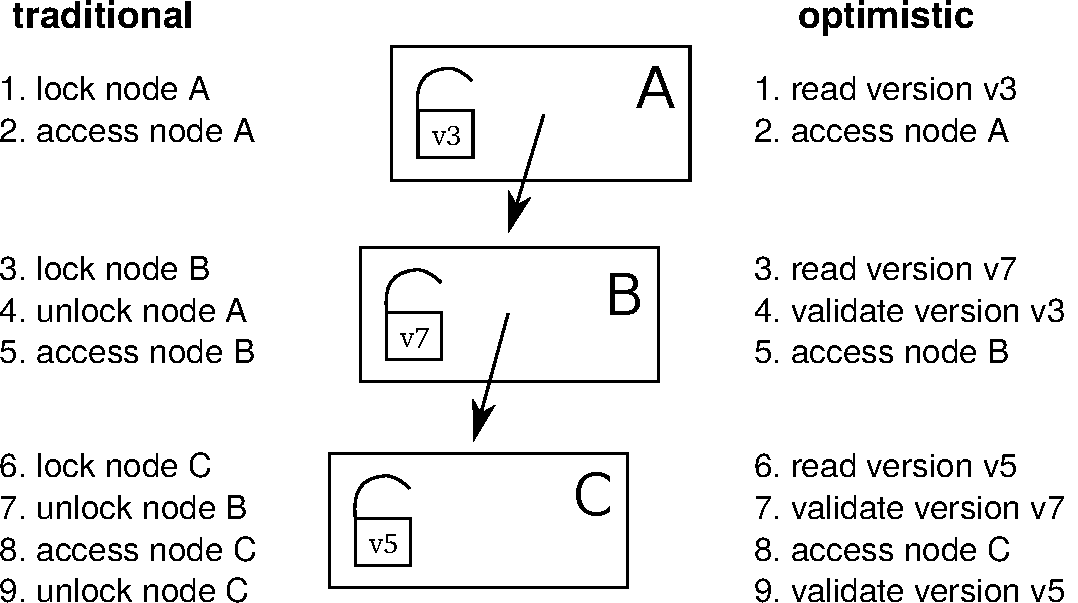
\includegraphics[width=0.65\linewidth]{olcall.pdf}
  \vspace{0.2cm}
  \caption{Comparison of a lookup operation in a 3-level tree using traditional lock coupling (left-hand side) vs.~optimistic lock coupling (right-hand side).}
  \label{fig:olc}
\end{figure}

The traditional and most common lock-based synchronization protocol for B-trees is lock coupling, which interleaves lock acquisitions while holding at most two locks at a time.
If, as we observed earlier, optimistic locks have similar semantics as traditional locks, it is natural to ask whether lock coupling can be combined with optimistic locks.
And indeed the answer is yes: One can almost mechanically translate traditional lock coupling code to optimistic lock coupling code.
This is illustrated in Figure~\ref{fig:olc}, which compares the traversal in a tree of height 3 using traditional and optimistic locks.
As the figure shows, the main difference is that locking is translated to reading the version and that unlocking becomes validation of the previously read version.
This simple change provides efficient lock-free tree traversal without the need to design a complex synchronization protocol.

It is important to emphasize the conceptual simplicity of OLC in comparison to data structures that use custom protocols like the Bw-tree~\cite{DBLP:conf/icde/LevandoskiLS13a}.
To implement lock-free access, the Bw-tree requires an indirection table, delta nodes, complex splitting and merging logic, retry logic, etc.
OLC, on the other hand, can directly be applied to B-trees mostly by adding the appropriate optimistic locking code and without modifying the node layout itself.
Therefore, OpenBw-Tree, an open source implementation of the Bw-tree, requires an order of magnitude more code than a B-tree based on OLC\footnote{Both implementations are available on GitHub: \url{https://github.com/wangziqi2016/index-microbench}}.
Given how difficult it is to develop, validate, and debug lock-free code, simplicity is obviously a major advantage.

\subsection{Correctness Aspects}

\begin{figure}
  % \centering
  %[basicstyle=\normalsize\ttfamily,showstringspaces=false,columns=fullflexible,breaklines=false,breakatwhitespace=true,numbers=none,numberstyle=\small,style=C,keepspaces=true]
\begin{lstlisting}[basicstyle=\ttfamily,language=C++,numbers=left,numberstyle=\small]
std::atomic<BTreeNode*> root;

// search for key in B+tree, returns payload in resultOut
bool lookup(Key key, Value& resultOut) {
   BTreeNode* node = root.load();
   uint64_t nodeVersion = node->readLockOrRestart();
   if (node != root.load()) // make sure the root is still the root
      restart();

   BTreeInner<Key>* parent = nullptr;
   uint64_t parentVersion = 0;

   while (node->isInner()) {
      auto inner = (BTreeInner*)node;

      // unlock parent and make current node the parent
      if (parent)
         parent->readUnlockOrRestart(parentVersion);
      parent = inner;
      parentVersion = nodeVersion;

      // search for next node
      node = inner->findChild(key);
      // validate 'inner' to ensure that 'node' pointer is valid
      inner->checkOrRestart(nodeVersion);
      // now it safe to dereference 'node' pointer (read its version)
      nodeVersion = node->readLockOrRestart();
   }

   // search in leaf and retrieve payload
   auto leaf = (BTreeLeaf*)node;
   bool success = leaf->findValue(key, resultOut);

   // unlock everything
   if (parent)
      parent->readUnlockOrRestart(parentVersion);
   node->readUnlockOrRestart(nodeVersion);

   return success;
}
\end{lstlisting}
  \vspace{0.2cm}
  \caption{B-tree lookup code using OLC. For simplicity, the restart logic is not shown.}
  \label{fig:lookup}
\end{figure}

So far, we have introduced the high-level ideas behind OLC and have stressed its similarity to traditional lock coupling.
Let us now discuss some cases where the close similarity between lock coupling and OLC breaks down.
To make this more concrete, we show the B-tree lookup code in Figure~\ref{fig:lookup}.
In the code, \texttt{readLockOrRestart} reads the lock version and \texttt{readUnlockOrRestart} validates that the read was correct.

One issue with OLC is that any pointer speculatively read from a node may point to invalid memory (if that node is modified concurrently).
Dereferencing such a pointer (e.g., to read its optimistic lock), may cause a segmentation fault or undefined behavior.
In the code shown in Figure~\ref{fig:lookup}, this problem is prevented by the extra check in line 25, which ensures that the read from the node containing the pointer was correct.
Without this additional validation, the code would in line 27 dereference the pointer speculatively read in line 23.
Note that the implementation of \texttt{checkOrRestart} is actually identical to \texttt{readUnlockOrRestart}.
We chose to give it a different name to highlight the fact that this extra check would not be necessary with read/write locks.

Another potential issue with optimistic locks is code that does not terminate.
Code that speculatively accesses a node, like an intra-node binary search, should be written in a way such that it always terminates---even in the presence of concurrent writes.
Otherwise, the validation code that detects the concurrent write will never run.
The binary search of a B-tree, for example, needs to be written in such a way that each comparison makes progress.
For some data structures that do not require loops in the traversal code (like ART) termination is trivially true.

\subsection{Implementation Details}

% implementation, efficiency
To implement an optimistic lock, one can combine the lock and the version counter into a single 64-bit\footnote{Even after subtracting one bit for the lock status, a back-of-the-envelope calculation can show that 63 bits are large enough to never overflow in practice.} word~\cite{artsync}.
A typical read operation will therefore merely consist of reading this version counter atomically.
In C++11 this can be implemented using the \texttt{std::atomic} type.

On x86, atomic reads are cheap because of x86's strong memory order guarantees.
No memory fences are required for sequentially-consistent loads, which are translated (by both GCC and clang) into standard \texttt{MOV} instructions.
Hence, the only effect of \texttt{std::atomic} for loads is preventing instruction re-ordering.
This makes version access and validation cheap.
Acquiring and releasing an optimistic lock in exclusive mode has comparable cost to a traditional lock:
A fairly expensive sequentially-consistent store is needed for acquiring a lock, while a standard \texttt{MOV} suffices for releasing it.
A simple sinlock-based implementation of optimistic locks can be found in the appendix of an earlier paper~\cite{artsync}.

OLC code must be able to handle restarts since validation or lock upgrade can fail due to concurrent writers.
Restarts can easily be implemented by wrapping the data structure operation in a loop (for simplicity not shown in Figure~\ref{fig:lookup}).
Such a loop also enables limiting the number of optimistic retry operations and falling back to pessimistic locking in cases of very heavy contention.
The ability to fall back to traditional locking is a major advantage of OLC in terms of robustness over lock-free approaches, which do not have this option.

In addition to the optimistic shared mode and the exclusive mode, optimistic locks also support a ``shared pessimistic'' mode, which physically acquires the lock in shared mode (allowing multiple concurrent readers but no writers).
This mode is useful for table (or range) scans that touch many tuples on a leaf page (which would otherwise easily abort).
Finally, let us mention that large range scans and table scans, should be broken up into several per-node traversals as is done in the LeanStore~\cite{leanstore} system.

Like all lock-free data structures, but unlike traditional locking and Hardware Transactional Memory~\cite{DBLP:conf/hpca/KarnagelDRLLSL14,DBLP:journals/pvldb/MakreshanskiLS15,htmtkde}, OLC requires care when deleting (and reusing) nodes.
The reason is that a deleting thread can never be sure that a node can be reclaimed because other threads might still be optimistically reading from that node.
Therefore, standard solutions like epoch-based reclamation~\cite{DBLP:conf/sosp/TuZKLM13}, hazard pointers~\cite{DBLP:journals/tpds/Michael04}, or optimized hazard pointers~\cite{DBLP:conf/spaa/BalmauGHZ16} need to be used.
These memory reclamation techniques are, however, largely orthogonal to the synchronization protocol itself.

%-lock-free is not a strong guarantee

\newpage
\section{Evaluation}\label{sec:evaluation}

Let us now experimentally evaluate the overhead and scalability of OLC.
For the experiments, we use an in-memory B+tree implemented in C++11 using templates, which is configured to use nodes of 4096 bytes, random 8 byte keys, and 8 byte payloads.
Based on this B-tree, we compare the following synchronization approaches:
\begin{itemize}
\item an OLC implementation\footnote{An almost identical OLC implementation is available on github: \url{https://github.com/wangziqi2016/index-microbench/tree/master/BTreeOLC}}
\item a variant based on traditional lock coupling and read/write locks
\item the unsynchronized B-tree, which obviously is only correct for read-only workloads but allows measuring the overhead of synchronization
\end{itemize}
Note that earlier work has compared the OLC implementation with a Bw-tree implementation~\cite{buzzword} and other state-of-the-art in-memory index structures.

We use a Haswell EP system with an Intel Xeon E5-2687W v3 CPU, which has 10 cores (20 ``Hyper-Threads'') and 25~MB of L3 cache.
The system is running Ubuntu 18.10 and we use GCC 8.2.0 to compile our code.
The CPU counters are obtained using the Linux perf API\footnote{We use the following convenience wrapper: \url{https://github.com/viktorleis/perfevent}}.

\begin{table}
  \caption{Performance and CPU counters for lookup and insert operations in a B-tree with 100M keys. We perform 100M operations and normalize the CPU counters by that number.}
  \label{tab:overhead}
  \centering
  \begin{tabular}{lrrrrrrr}\toprule
                    &         &        &        & instruc-  & L1     & L3     & branch \\
                    & threads & M op/s & cycles & tions & misses & misses & misses \\\midrule
lookup (no sync.)   & 1       & 1.72   & 2028   & 283     & 39.1   & 14.9   & 16.1   \\
lookup (OLC)        & 1       & 1.65   & 2107   & 370     & 43.9   & 15.1   & 16.7   \\
lookup (lock coup.) & 1       & 1.72   & 2078   & 365     & 42.3   & 16.9   & 15.7   \\\midrule
insert (no sync.)   & 1       & 1.51   & 2286   & 530     & 59.8   & 31.1   & 17.3   \\
insert (OLC)        & 1       & 1.50   & 2303   & 629     & 61.2   & 31.1   & 16.5   \\
insert (lock coup.) & 1       & 1.41   & 2473   & 644     & 61.0   & 31.0   & 17.2   \\\midrule
lookup (no sync.)   & 10      & 15.48  & 2058   & 283     & 38.6   & 15.5   & 16.0   \\
lookup (OLC)        & 10      & 14.60  & 2187   & 370     & 43.8   & 15.8   & 16.8   \\
lookup (lock coup.) & 10      & 5.71   & 5591   & 379     & 54.2   & 17.0   & 14.8   \\\midrule
insert (no sync.)   & 10      & -      & -      & -       & -      & -      & -      \\
insert (OLC)        & 10      & 10.46  & 2940   & 656     & 62.0   & 32.5   & 16.8   \\
insert (lock coup.) & 10      & 7.55   & 4161   & 667     & 75.0   & 28.6   & 16.2   \\
    \bottomrule
\end{tabular}
\end{table}

Table~\ref{tab:overhead} compares the performance and CPU counters for lookup and insert operations in a B-tree with 100M keys.
With {\em single-threaded} execution, we observe that all three approaches have very similar performance.
Adding traditional or optimistic locks to unsynchronized B-tree code results in up to 30\% of additional instructions without affecting single-threaded performance much.

\begin{figure}
  \centering
  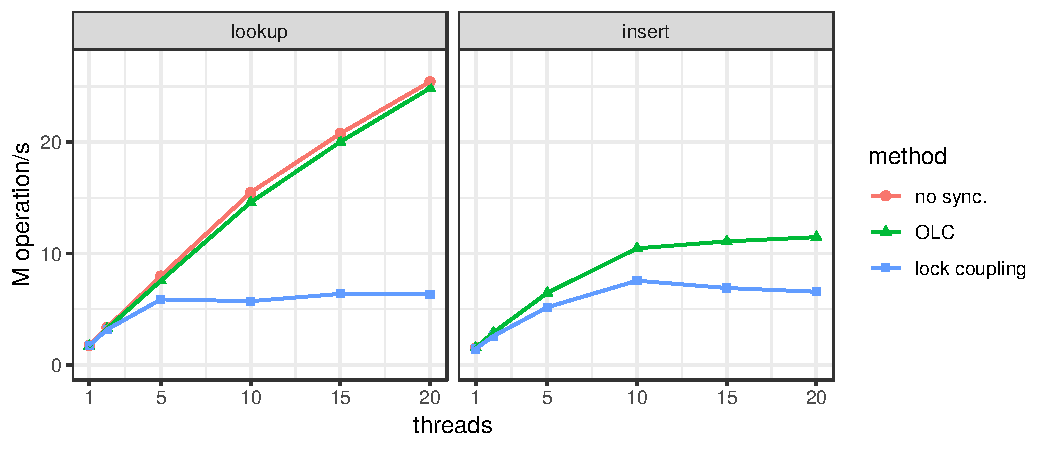
\includegraphics[width=\linewidth]{scale.pdf}
  \vspace{0.2cm}
  \caption{Scalability on 10-core system for B-tree operations (100M values).}
  \label{fig:scale}
\end{figure}

As Figure~\ref{fig:scale} shows, the results change dramatically once we use multiple threads.
For lookup, the scalability of OLC is near-linear up to 20 threads, even though the system has only 10 ``real cores''.
The OLC scalability for insert is also respectable (though not quite as linear because multi-threaded insertion approaches the memory bandwidth of our processor).
The figure also shows that the results of traditional lock coupling with read/write locks are significantly worse than OLC.
With 20 threads, lookup with OLC is 3.9$\times$ faster than traditional lock coupling.

\section{Summary}\label{sec:conc}

Optimistic Lock Coupling (OLC) is an effective synchronization method that combines the simplicity of traditional lock coupling with the superior scalability of lock-free approaches.
OLC is widely applicable and has already been successfully used to synchronize several data structures, including B-trees, binary search trees, and different trie variants.
These features make it highly attractive for modern database systems as well as performance-critical systems software in general.

\begin{thebibliography}{10}

\bibitem{DBLP:conf/spaa/BalmauGHZ16}
O.~Balmau, R.~Guerraoui, M.~Herlihy, and I.~Zablotchi.
\newblock Fast and robust memory reclamation for concurrent data structures.
\newblock In {\em SPAA}, 2016.

\bibitem{DBLP:journals/acta/BayerS77}
R.~Bayer and M.~Schkolnick.
\newblock Concurrency of operations on {B}-trees.
\newblock {\em Acta Informatica}, 9, 1977.

\bibitem{hot}
R.~Binna, E.~Zangerle, M.~Pichl, G.~Specht, and V.~Leis.
\newblock {HOT}: A height optimized trie index for main-memory database
  systems.
\newblock In {\em SIGMOD}, 2018.

\bibitem{DBLP:conf/ppopp/BronsonCCO10}
N.~G. Bronson, J.~Casper, H.~Chafi, and K.~Olukotun.
\newblock A practical concurrent binary search tree.
\newblock In {\em PPOPP}, 2010.

\bibitem{DBLP:conf/vldb/ChaHKK01}
S.~K. Cha, S.~Hwang, K.~Kim, and K.~Kwon.
\newblock Cache-conscious concurrency control of main-memory indexes on
  shared-memory multiprocessor systems.
\newblock In {\em VLDB}, 2001.

\bibitem{intel}
I.~Cutress.
\newblock {Intel} goes for 48-cores: {Cascade-AP} with multi-chip package
  coming soon.
\newblock
  \url{https://www.anandtech.com/show/13535/intel-goes-for-48cores-cascade-ap},
  2018 (accessed January, 2019).

\bibitem{DBLP:conf/cidr/FaleiroA17}
J.~M. Faleiro and D.~J. Abadi.
\newblock Latch-free synchronization in database systems: Silver bullet or
  fool's gold?
\newblock In {\em CIDR}, 2017.

\bibitem{DBLP:journals/ftdb/Graefe11}
G.~Graefe.
\newblock Modern {B}-tree techniques.
\newblock {\em Foundations and Trends in Databases}, 3(4), 2011.

\bibitem{DBLP:conf/hpca/KarnagelDRLLSL14}
T.~Karnagel, R.~Dementiev, R.~Rajwar, K.~Lai, T.~Legler, B.~Schlegel, and
  W.~Lehner.
\newblock Improving in-memory database index performance with
  {Intel}\({}^{\mbox{{\textregistered}}}\) transactional synchronization
  extensions.
\newblock In {\em HPCA}, 2014.

\bibitem{DBLP:journals/tods/LehmanY81}
P.~L. Lehman and S.~B. Yao.
\newblock Efficient locking for concurrent operations on {B}-trees.
\newblock {\em {ACM} Trans. Database Syst.}, 6(4), 1981.

\bibitem{leanstore}
V.~Leis, M.~Haubenschild, A.~Kemper, and T.~Neumann.
\newblock Leanstore: In-memory data management beyond main memory.
\newblock In {\em ICDE}, 2018.

\bibitem{art}
V.~Leis, A.~Kemper, and T.~Neumann.
\newblock The adaptive radix tree: {ARTful} indexing for main-memory databases.
\newblock In {\em ICDE}, 2013.

\bibitem{htmtkde}
V.~Leis, A.~Kemper, and T.~Neumann.
\newblock Scaling {HTM}-supported database transactions to many cores.
\newblock {\em {IEEE} Trans. Knowl. Data Eng.}, 28(2), 2016.

\bibitem{artsync}
V.~Leis, F.~Scheibner, A.~Kemper, and T.~Neumann.
\newblock The {ART} of practical synchronization.
\newblock In {\em DaMoN}, 2016.

\bibitem{DBLP:conf/icde/LevandoskiLS13a}
J.~J. Levandoski, D.~B. Lomet, and S.~Sengupta.
\newblock The {Bw}-tree: A {B}-tree for new hardware platforms.
\newblock In {\em ICDE}, 2013.

\bibitem{DBLP:journals/pvldb/MakreshanskiLS15}
D.~Makreshanski, J.~J. Levandoski, and R.~Stutsman.
\newblock To lock, swap, or elide: On the interplay of hardware transactional
  memory and lock-free indexing.
\newblock {\em {PVLDB}}, 8(11), 2015.

\bibitem{DBLP:dblp_conf/eurosys/MaoKM12}
Y.~Mao, E.~Kohler, and R.~T. Morris.
\newblock Cache craftiness for fast multicore key-value storage.
\newblock In {\em EuroSys}, 2012.

\bibitem{DBLP:journals/tpds/Michael04}
M.~M. Michael.
\newblock Hazard pointers: Safe memory reclamation for lock-free objects.
\newblock {\em {IEEE} Trans. Parallel Distrib. Syst.}, 15(6), 2004.

\bibitem{DBLP:journals/jacm/ShalevS06}
O.~Shalev and N.~Shavit.
\newblock Split-ordered lists: Lock-free extensible hash tables.
\newblock {\em J. {ACM}}, 53(3), 2006.

\bibitem{amd}
A.~Shilov.
\newblock {AMD} previews {EPYC} ‘{Rome}’ processor: Up to 64 {Zen} 2 cores.
\newblock
  \url{https://www.anandtech.com/show/13561/amd-previews-epyc-rome-processor-up-to-64-zen-2-cores},
  2018 (accessed January, 2019).

\bibitem{DBLP:conf/sosp/TuZKLM13}
S.~Tu, W.~Zheng, E.~Kohler, B.~Liskov, and S.~Madden.
\newblock Speedy transactions in multicore in-memory databases.
\newblock In {\em SOSP}, 2013.

\bibitem{buzzword}
Z.~Wang, A.~Pavlo, H.~Lim, V.~Leis, H.~Zhang, M.~Kaminsky, and D.~Andersen.
\newblock Building a {Bw}-tree takes more than just buzz words.
\newblock In {\em SIGMOD}, 2018.

\end{thebibliography}


%\bibliographystyle{abbrv}
%\bibliography{main}

\end{document}

\end{article}

\end{articlesection}


% put the news items below- there can be multiple news sections
% each with its own title
% news will usually have an author as well as a title,
% e.g. TCDE elections
% news articles are in the same format as lett ers
% typically, news articles will be stored in a directory called "news"


% \begin{newssection}{Obituary}
% \begin{news}{Obituary for Professor Gio Wiederhold}
% {Kyu-Young Whang and Marianne Winslett}{Distinguished Professor Emeritus, KAIST\\ Research Professor Emerita, UIUC\\ together with Gio’s other former students}
% \documentclass[11pt]{article} 

\usepackage{deauthor,times,graphicx}
%\usepackage{url}
\usepackage{hyperref}

\begin{document}
%Obituary for Professor Gio Wiederhold
%                                                                  December 26, 2022                                                                         
Professor Gio Wiederhold passed away in the early hours of December 26, 2022, aged 86, just 10 weeks after an unexpected diagnosis of stage 4 liver cancer. Gio died at home, surrounded by his family members who had gathered for Christmas, including his wife of 56 years, Voy Wiederhold, and his sons John and Randy.  


Gio was a great scholar, educator, and mentor. His influence on the database field is immense. As a pioneer in the database field, he wrote the influential 1977 textbook Database Design, one of the first in the field and adopted around the world. In his DARPA-supported Knowledge-Base Management Systems project in the early 1980s, Gio pioneered the concept of integrating databases and AI, a topic that is now enjoying a revival. Beginning in the 1970s, Gio also pursued the application of databases to medical informatics, another area just now entering the mainstream. In 1992, Gio introduced the notion of mediators (IEEE Computer) as a way of intelligently integrating information from large-scale heterogeneous sources such as databases, file systems, and repositories, a seminal idea for the nascent field of information integration. Gio continued to innovate after retirement from Stanford, most notably in establishing an approach for valuing software and the intellectual property of multinational firms.


Gio advised 36 PhD students at Stanford. Today, Gio’s academic descendants can be found in companies and universities all over the world, including early students Hector Garcia-Molina (the late Stanford professor), David Shaw (DE Shaw founder), Ramez Elmasri (the late textbook author and UT Arlington professor), Kyu-Young Whang (KAIST professor and Naver founder’s advisor), and Marianne Winslett (UIUC professor). Gio’s many subsequent students continue to lead the database field today. 


An influential mentor, Gio always emphasized the practical aspects of research, encouraging people to develop both theoretical and engineering approaches to solve real-world problems. This outlook stemmed from his many years of experience in computing practice before he joined the Stanford University faculty.


Gio’s service to the professional community includes serving as the third Editor-in-Chief of ACM Transactions on Databases during 1985-1995, during which time he significantly contributed to making the new journal a top one in the field. Together with five colleagues, Gio co-founded the IEEE International Conference on Data Engineering in 1984. Perhaps the first venue to use the term data engineering, the conference was unique in focusing on engineering aspects of database research; today it stands as one of the three top-tier conferences in database research. Gio also served as the conference’s program committee chair, co-chair, and general chair in its early years. During 1991-1994, Gio served as the program manager for DARPA’s Knowledge-based Systems program, which collaborated with NSF to fund innovative new research related to information integration and digital libraries — including the project that led to the creation of Google.


In recognition of his many contributions, Gio received the IEEE Technical Community on Data Engineering’s Service Award in 2016. He was also a Fellow of the ACM, the IEEE, and the American College of Medical Informatics.




The many accomplishments and contributions listed above do not capture the full extent of Gio’s impact and influence on our community, nor his diligence and persistence. As Gio’s former students, we dearly miss him for his warm heart towards his students, colleagues, and friends, and above all, his love and kindness for everyone he knew. We are deeply saddened by Gio’s unexpected death and send our sincerest condolences to his surviving family and friends.  




%-- Kyu-Young Whang, Distinguished Professor Emeritus, KAIST and Marianne Winslett, Research Professor Emerita, University of Illinois at Urbana-Champaign, together with Gio’s other former students
\end{document}

% \end{news}

% \newpage
% \end{newssection}


\begin{callsection}

%  This section will be empty for your version
%
%  Calls for papers section.  Use the callsection environment.
%  Each call for papers is contained in an call environment, where the single
%  required options to \begin{call} is the name of the conference.
% typically calls are stored in a "calls" directory
%
%\begin{call}{name of conference}
%\centerline{\includegraphics[width=\textwidth, bb= 0 0 590 760]{calls/conference-name.pdf}}
%\end{call}
%\begin{call}{ICDE 2019 Conference}
%\centerline{
\includegraphics[width=\textwidth, bb= 0 0 610 790] {../Dec-2018/calls/icde19.pdf}}
%\centerline{
\includegraphics[width=\textwidth, bb= 0 0 590 760] {calls/icde19.pdf}}
%\end{call}
\begin{call}{TCDE Membership Form}
%\centerline{\includegraphics[width=\textwidth, bb= 0 0 610 790]
%\centerline{
\includegraphics[width=\textwidth, bb= 0 0 590 760] {../Dec-2018/calls/tcde.pdf}}
\centerline{
\includegraphics[width=\textwidth, bb= 0 0 590 760] {./calls/tcde.pdf}}
\end{call}

\end{callsection}

\end{bulletin}
\end{document}
